\documentclass[t]{beamer}
%\documentclass[finnish,english,handout]{beamer}

\usepackage{tikz}
\usepackage{bm}
\usepackage[T1]{fontenc}
\usepackage{booktabs}
\usepackage[utf8]{inputenc}
\usepackage{newtxtext} % times
%\usepackage[scaled=.95]{cabin} % sans serif
\usepackage{amsmath}
\usepackage[varqu,varl]{inconsolata} % typewriter
\usepackage[varg]{newtxmath}
\usefonttheme[onlymath]{serif} % beamer font theme
\usepackage{microtype}
\usepackage{afterpage}
\usepackage{url}
\urlstyle{same}
% \usepackage{amsbsy}
% \usepackage{eucal}
\usepackage{rotating}
\usepackage{listings}
\usepackage{lstbayes}
\usepackage[all,poly,ps,color]{xy}
\usepackage{eurosym}

\usepackage{natbib}
\bibliographystyle{apalike}

\mode<presentation>
{
  \setbeamercovered{invisible}
  \setbeamertemplate{itemize items}[circle]
  \setbeamercolor{frametitle}{bg=white,fg=navyblue}
  \setbeamertemplate{navigation symbols}{}
  \setbeamertemplate{headline}[default]{}
  \setbeamertemplate{footline}[split]
  % \setbeamertemplate{headline}[text line]{\insertsection}
  \setbeamertemplate{footline}[frame number]
}

\pdfinfo{            
  /Title      (BDA, Lecture 11a) 
  /Author     (Aki Vehtari) % 
  /Keywords   (Bayesian data analysis)
}

\definecolor{forestgreen}{rgb}{0.1333,0.5451,0.1333}
\definecolor{navyblue}{rgb}{0,0,0.5}
\definecolor{list1}{rgb}{0,0.2549,0.6784}
\renewcommand{\emph}[1]{\textcolor{navyblue}{#1}}
\definecolor{set11}{HTML}{E41A1C}
\definecolor{set12}{HTML}{377EB8}
\definecolor{set13}{HTML}{4DAF4A}
\definecolor{prior}{RGB}{102,194,165}
\definecolor{likelihood}{RGB}{252,141,98}

\graphicspath{{./figs/}}


\parindent=0pt
\parskip=8pt
\tolerance=9000
\abovedisplayshortskip=0pt

%\renewcommand{\itemsep}{0pt}
% Lists
\newenvironment{list1}{
   \begin{list}{$\color{list1}\bullet$}{\itemsep=6pt}}{
  \end{list}}
\newenvironment{list1s}{
  \begin{list}{$\includegraphics[width=5pt]{logo.eps}$}{\itemsep=6pt}}{
  \end{list}}
\newenvironment{list2}{
  \begin{list}{-}{\baselineskip=12pt\itemsep=2pt}}{
  \end{list}}
\newenvironment{list3}{
  \begin{list}{$\cdot$}{\baselineskip=15pt}}{
  \end{list}}

\def\o{{\mathbf o}}
\def\t{{\mathbf \theta}}
\def\w{{\mathbf w}}
\def\x{{\mathbf x}}
\def\y{{\mathbf y}}
\def\z{{\mathbf z}}

\def\peff{p_{\mathrm{eff}}}
\def\eff{\mathrm{eff}}

\DeclareMathOperator{\E}{E}
\DeclareMathOperator{\Var}{Var}
\DeclareMathOperator{\var}{var}
\DeclareMathOperator{\Sd}{Sd}
\DeclareMathOperator{\sd}{sd}
\DeclareMathOperator{\Gammad}{Gamma}
\DeclareMathOperator{\Invgamma}{Inv-gamma}
\DeclareMathOperator{\Bin}{Bin}
\DeclareMathOperator{\Negbin}{Neg-bin}
\DeclareMathOperator{\normal}{normal}
\DeclareMathOperator{\gammadist}{gamma}
\DeclareMathOperator{\expdist}{exponential}
\DeclareMathOperator{\Poisson}{Poisson}
\DeclareMathOperator{\betadist}{Beta}
\DeclareMathOperator{\logit}{logit}
\DeclareMathOperator{\N}{N}
\DeclareMathOperator{\U}{U}
\DeclareMathOperator{\BF}{BF}
\DeclareMathOperator{\Invchi2}{Inv-\chi^2}
\DeclareMathOperator{\NInvchi2}{N-Inv-\chi^2}
\DeclareMathOperator{\InvWishart}{Inv-Wishart}
\DeclareMathOperator{\tr}{tr}
% \DeclareMathOperator{\Pr}{Pr}
\def\euro{{\footnotesize \EUR\, }}
\DeclareMathOperator{\rep}{\mathrm{rep}}

% \def\dashxy(#1){%
%   /xydash{[#1] 0 setdash}def}
% \def\grayxy(#1){%
%   /xycolor{#1 setgray}def}
% \newgraphescape{D}[1]{!{\ar @*{[!\dashxy(2 2)]} "#1"}}
% \newgraphescape{P}[1]{!{\ar "#1"}}
% \newgraphescape{F}[1]{!{*+=<2em>[F=]{#1}="#1"}}
% \newgraphescape{O}[1]{!{*+=<2em>[F]{#1}="#1"}}
% \newgraphescape{V}[1]{!{*+=<2em>[o][F]{#1}="#1"}}
% \newgraphescape{B}[3]{!{{ "#1"*+#3\frm{} }.{ "#2"*+#3\frm{} } *+[F:!\grayxy(0.75)]\frm{}}}


\title[]{Bayesian data analysis}
\subtitle{}

\author{Noa Kallioinen}

\institute[Aalto]{}
 
\date[]{}

%\beamerdefaultoverlayspecification{<+->}

\begin{document}

%\maketitle

\begin{frame}{Prior and likelihood sensitivity checks with priorsense}

\begin{itemize}[<+->]
\item sensible prior specification is important, as otherwise priors can strongly and unintentionally influence results
\item we recommend checking prior and likelihood sensitivity using priorsense (Kallioinen et al., 2023)
\end{itemize}

\begin{minipage}{0.2\textwidth}
\onslide<2->{\begin{figure}
\includegraphics[width=\textwidth]{logo.png}
\end{figure}}
\end{minipage}
\hspace{0.05\textwidth}
\begin{minipage}{0.65\textwidth}
\begin{itemize}[<+->]
    \item efficient prior and likelihood sensitivity checks
    \item provides numerical and graphical diagnostics
    \item compatible with \texttt{brms} and applicable to any model (excluding flat priors)
    \item no need to refit
\end{itemize}

\end{minipage}

\end{frame}

\begin{frame}{How it works}
\begin{minipage}{0.2\textwidth}
\begin{figure}
    \includegraphics[width=\linewidth]{logo.png}
\end{figure}
\end{minipage}
\hspace{0.05\textwidth}
\begin{minipage}{0.65\textwidth}
\begin{itemize}[<+->]
\item modifies the posterior by power-scaling the \textcolor{prior}{\textbf{prior}} or \textcolor{likelihood}{\textbf{likelihood}} slightly
        \item original posterior: \(p(\theta\mid y) \propto p(\theta)p(y\mid \theta)\)
    \item modified posterior: \(\bm{{\color{prior}{p(\theta)^{\alpha}}}} p(y\mid \theta)\) or \(p(\theta) 
    \bm{{\color{likelihood}{p(y\mid \theta)^{\alpha}}}}\)
    \item uses Pareto-smoothed importance sampling to estimate modified posterior from original posterior draws \(\theta^{(s)}\)
 
\end{itemize}
\end{minipage}
\end{frame}

\begin{frame}{Power-scaling}
\begin{figure}
    \centering
% Created by tikzDevice version 0.12.3.1 on 2022-05-05 12:56:25
% !TEX encoding = UTF-8 Unicode
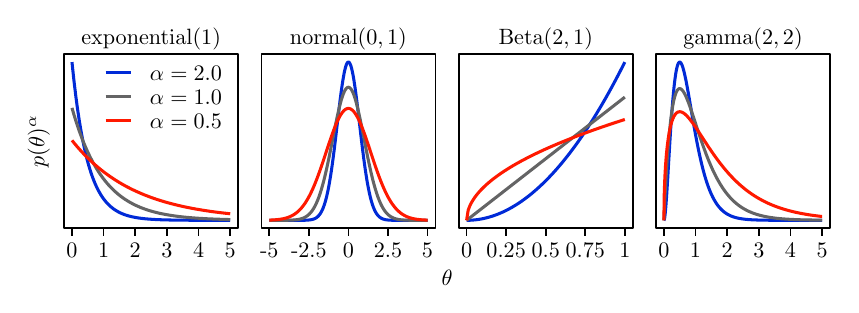
\begin{tikzpicture}[scale=0.8,transform shape,x=1pt,y=1pt]
\definecolor{fillColor}{RGB}{255,255,255}
\begin{scope}
\definecolor{drawColor}{RGB}{0,42,215}

\path[draw=drawColor,line width= 1.1pt,line join=round] ( 26.41,229.55) --
	( 26.55,228.14) --
	( 26.69,226.75) --
	( 26.84,225.39) --
	( 26.98,224.06) --
	( 27.12,222.75) --
	( 27.26,221.47) --
	( 27.41,220.22) --
	( 27.55,218.99) --
	( 27.69,217.78) --
	( 27.84,216.60) --
	( 27.98,215.44) --
	( 28.12,214.30) --
	( 28.26,213.19) --
	( 28.41,212.10) --
	( 28.55,211.03) --
	( 28.69,209.98) --
	( 28.84,208.95) --
	( 28.98,207.95) --
	( 29.12,206.96) --
	( 29.27,205.99) --
	( 29.41,205.04) --
	( 29.55,204.11) --
	( 29.69,203.20) --
	( 29.84,202.31) --
	( 29.98,201.43) --
	( 30.12,200.57) --
	( 30.27,199.73) --
	( 30.41,198.91) --
	( 30.55,198.10) --
	( 30.69,197.31) --
	( 30.84,196.53) --
	( 30.98,195.77) --
	( 31.12,195.02) --
	( 31.27,194.29) --
	( 31.41,193.57) --
	( 31.55,192.87) --
	( 31.70,192.18) --
	( 31.84,191.51) --
	( 31.98,190.84) --
	( 32.12,190.20) --
	( 32.27,189.56) --
	( 32.41,188.94) --
	( 32.55,188.33) --
	( 32.70,187.73) --
	( 32.84,187.14) --
	( 32.98,186.56) --
	( 33.12,186.00) --
	( 33.27,185.45) --
	( 33.41,184.90) --
	( 33.55,184.37) --
	( 33.70,183.85) --
	( 33.84,183.34) --
	( 33.98,182.84) --
	( 34.13,182.35) --
	( 34.27,181.87) --
	( 34.41,181.40) --
	( 34.55,180.94) --
	( 34.70,180.49) --
	( 34.84,180.04) --
	( 34.98,179.61) --
	( 35.13,179.18) --
	( 35.27,178.76) --
	( 35.41,178.35) --
	( 35.55,177.95) --
	( 35.70,177.56) --
	( 35.84,177.17) --
	( 35.98,176.80) --
	( 36.13,176.42) --
	( 36.27,176.06) --
	( 36.41,175.71) --
	( 36.56,175.36) --
	( 36.70,175.01) --
	( 36.84,174.68) --
	( 36.98,174.35) --
	( 37.13,174.03) --
	( 37.27,173.71) --
	( 37.41,173.40) --
	( 37.56,173.10) --
	( 37.70,172.80) --
	( 37.84,172.51) --
	( 37.98,172.22) --
	( 38.13,171.94) --
	( 38.27,171.67) --
	( 38.41,171.40) --
	( 38.56,171.14) --
	( 38.70,170.88) --
	( 38.84,170.63) --
	( 38.99,170.38) --
	( 39.13,170.13) --
	( 39.27,169.89) --
	( 39.41,169.66) --
	( 39.56,169.43) --
	( 39.70,169.21) --
	( 39.84,168.99) --
	( 39.99,168.77) --
	( 40.13,168.56) --
	( 40.27,168.35) --
	( 40.41,168.15) --
	( 40.56,167.95) --
	( 40.70,167.75) --
	( 40.84,167.56) --
	( 40.99,167.37) --
	( 41.13,167.19) --
	( 41.27,167.01) --
	( 41.42,166.83) --
	( 41.56,166.66) --
	( 41.70,166.49) --
	( 41.84,166.32) --
	( 41.99,166.16) --
	( 42.13,166.00) --
	( 42.27,165.84) --
	( 42.42,165.69) --
	( 42.56,165.54) --
	( 42.70,165.39) --
	( 42.84,165.25) --
	( 42.99,165.10) --
	( 43.13,164.96) --
	( 43.27,164.83) --
	( 43.42,164.69) --
	( 43.56,164.56) --
	( 43.70,164.44) --
	( 43.85,164.31) --
	( 43.99,164.19) --
	( 44.13,164.07) --
	( 44.27,163.95) --
	( 44.42,163.83) --
	( 44.56,163.72) --
	( 44.70,163.61) --
	( 44.85,163.50) --
	( 44.99,163.39) --
	( 45.13,163.28) --
	( 45.27,163.18) --
	( 45.42,163.08) --
	( 45.56,162.98) --
	( 45.70,162.88) --
	( 45.85,162.79) --
	( 45.99,162.70) --
	( 46.13,162.60) --
	( 46.28,162.51) --
	( 46.42,162.43) --
	( 46.56,162.34) --
	( 46.70,162.26) --
	( 46.85,162.17) --
	( 46.99,162.09) --
	( 47.13,162.01) --
	( 47.28,161.93) --
	( 47.42,161.86) --
	( 47.56,161.78) --
	( 47.70,161.71) --
	( 47.85,161.64) --
	( 47.99,161.57) --
	( 48.13,161.50) --
	( 48.28,161.43) --
	( 48.42,161.36) --
	( 48.56,161.30) --
	( 48.71,161.24) --
	( 48.85,161.17) --
	( 48.99,161.11) --
	( 49.13,161.05) --
	( 49.28,160.99) --
	( 49.42,160.94) --
	( 49.56,160.88) --
	( 49.71,160.82) --
	( 49.85,160.77) --
	( 49.99,160.72) --
	( 50.13,160.66) --
	( 50.28,160.61) --
	( 50.42,160.56) --
	( 50.56,160.51) --
	( 50.71,160.47) --
	( 50.85,160.42) --
	( 50.99,160.37) --
	( 51.14,160.33) --
	( 51.28,160.28) --
	( 51.42,160.24) --
	( 51.56,160.20) --
	( 51.71,160.15) --
	( 51.85,160.11) --
	( 51.99,160.07) --
	( 52.14,160.03) --
	( 52.28,159.99) --
	( 52.42,159.96) --
	( 52.56,159.92) --
	( 52.71,159.88) --
	( 52.85,159.85) --
	( 52.99,159.81) --
	( 53.14,159.78) --
	( 53.28,159.74) --
	( 53.42,159.71) --
	( 53.57,159.68) --
	( 53.71,159.65) --
	( 53.85,159.62) --
	( 53.99,159.59) --
	( 54.14,159.56) --
	( 54.28,159.53) --
	( 54.42,159.50) --
	( 54.57,159.47) --
	( 54.71,159.44) --
	( 54.85,159.42) --
	( 54.99,159.39) --
	( 55.14,159.36) --
	( 55.28,159.34) --
	( 55.42,159.31) --
	( 55.57,159.29) --
	( 55.71,159.26) --
	( 55.85,159.24) --
	( 56.00,159.22) --
	( 56.14,159.20) --
	( 56.28,159.17) --
	( 56.42,159.15) --
	( 56.57,159.13) --
	( 56.71,159.11) --
	( 56.85,159.09) --
	( 57.00,159.07) --
	( 57.14,159.05) --
	( 57.28,159.03) --
	( 57.42,159.01) --
	( 57.57,158.99) --
	( 57.71,158.98) --
	( 57.85,158.96) --
	( 58.00,158.94) --
	( 58.14,158.92) --
	( 58.28,158.91) --
	( 58.43,158.89) --
	( 58.57,158.87) --
	( 58.71,158.86) --
	( 58.85,158.84) --
	( 59.00,158.83) --
	( 59.14,158.81) --
	( 59.28,158.80) --
	( 59.43,158.78) --
	( 59.57,158.77) --
	( 59.71,158.76) --
	( 59.85,158.74) --
	( 60.00,158.73) --
	( 60.14,158.72) --
	( 60.28,158.70) --
	( 60.43,158.69) --
	( 60.57,158.68) --
	( 60.71,158.67) --
	( 60.86,158.66) --
	( 61.00,158.65) --
	( 61.14,158.63) --
	( 61.28,158.62) --
	( 61.43,158.61) --
	( 61.57,158.60) --
	( 61.71,158.59) --
	( 61.86,158.58) --
	( 62.00,158.57) --
	( 62.14,158.56) --
	( 62.28,158.55) --
	( 62.43,158.54) --
	( 62.57,158.53) --
	( 62.71,158.52) --
	( 62.86,158.52) --
	( 63.00,158.51) --
	( 63.14,158.50) --
	( 63.29,158.49) --
	( 63.43,158.48) --
	( 63.57,158.47) --
	( 63.71,158.47) --
	( 63.86,158.46) --
	( 64.00,158.45) --
	( 64.14,158.44) --
	( 64.29,158.44) --
	( 64.43,158.43) --
	( 64.57,158.42) --
	( 64.71,158.42) --
	( 64.86,158.41) --
	( 65.00,158.40) --
	( 65.14,158.40) --
	( 65.29,158.39) --
	( 65.43,158.38) --
	( 65.57,158.38) --
	( 65.72,158.37) --
	( 65.86,158.37) --
	( 66.00,158.36) --
	( 66.14,158.36) --
	( 66.29,158.35) --
	( 66.43,158.34) --
	( 66.57,158.34) --
	( 66.72,158.33) --
	( 66.86,158.33) --
	( 67.00,158.32) --
	( 67.14,158.32) --
	( 67.29,158.31) --
	( 67.43,158.31) --
	( 67.57,158.31) --
	( 67.72,158.30) --
	( 67.86,158.30) --
	( 68.00,158.29) --
	( 68.15,158.29) --
	( 68.29,158.28) --
	( 68.43,158.28) --
	( 68.57,158.28) --
	( 68.72,158.27) --
	( 68.86,158.27) --
	( 69.00,158.26) --
	( 69.15,158.26) --
	( 69.29,158.26) --
	( 69.43,158.25) --
	( 69.57,158.25) --
	( 69.72,158.25) --
	( 69.86,158.24) --
	( 70.00,158.24) --
	( 70.15,158.24) --
	( 70.29,158.23) --
	( 70.43,158.23) --
	( 70.58,158.23) --
	( 70.72,158.23) --
	( 70.86,158.22) --
	( 71.00,158.22) --
	( 71.15,158.22) --
	( 71.29,158.21) --
	( 71.43,158.21) --
	( 71.58,158.21) --
	( 71.72,158.21) --
	( 71.86,158.20) --
	( 72.00,158.20) --
	( 72.15,158.20) --
	( 72.29,158.20) --
	( 72.43,158.19) --
	( 72.58,158.19) --
	( 72.72,158.19) --
	( 72.86,158.19) --
	( 73.01,158.19) --
	( 73.15,158.18) --
	( 73.29,158.18) --
	( 73.43,158.18) --
	( 73.58,158.18) --
	( 73.72,158.18) --
	( 73.86,158.17) --
	( 74.01,158.17) --
	( 74.15,158.17) --
	( 74.29,158.17) --
	( 74.43,158.17) --
	( 74.58,158.16) --
	( 74.72,158.16) --
	( 74.86,158.16) --
	( 75.01,158.16) --
	( 75.15,158.16) --
	( 75.29,158.16) --
	( 75.44,158.15) --
	( 75.58,158.15) --
	( 75.72,158.15) --
	( 75.86,158.15) --
	( 76.01,158.15) --
	( 76.15,158.15) --
	( 76.29,158.15) --
	( 76.44,158.15) --
	( 76.58,158.14) --
	( 76.72,158.14) --
	( 76.86,158.14) --
	( 77.01,158.14) --
	( 77.15,158.14) --
	( 77.29,158.14) --
	( 77.44,158.14) --
	( 77.58,158.14) --
	( 77.72,158.13) --
	( 77.87,158.13) --
	( 78.01,158.13) --
	( 78.15,158.13) --
	( 78.29,158.13) --
	( 78.44,158.13) --
	( 78.58,158.13) --
	( 78.72,158.13) --
	( 78.87,158.13) --
	( 79.01,158.13) --
	( 79.15,158.12) --
	( 79.29,158.12) --
	( 79.44,158.12) --
	( 79.58,158.12) --
	( 79.72,158.12) --
	( 79.87,158.12) --
	( 80.01,158.12) --
	( 80.15,158.12) --
	( 80.30,158.12) --
	( 80.44,158.12) --
	( 80.58,158.12) --
	( 80.72,158.12) --
	( 80.87,158.12) --
	( 81.01,158.11) --
	( 81.15,158.11) --
	( 81.30,158.11) --
	( 81.44,158.11) --
	( 81.58,158.11) --
	( 81.72,158.11) --
	( 81.87,158.11) --
	( 82.01,158.11) --
	( 82.15,158.11) --
	( 82.30,158.11) --
	( 82.44,158.11) --
	( 82.58,158.11) --
	( 82.73,158.11) --
	( 82.87,158.11) --
	( 83.01,158.11) --
	( 83.15,158.11) --
	( 83.30,158.10) --
	( 83.44,158.10) --
	( 83.58,158.10) --
	( 83.73,158.10) --
	( 83.87,158.10) --
	( 84.01,158.10) --
	( 84.15,158.10) --
	( 84.30,158.10) --
	( 84.44,158.10) --
	( 84.58,158.10) --
	( 84.73,158.10) --
	( 84.87,158.10) --
	( 85.01,158.10) --
	( 85.16,158.10) --
	( 85.30,158.10) --
	( 85.44,158.10) --
	( 85.58,158.10) --
	( 85.73,158.10) --
	( 85.87,158.10) --
	( 86.01,158.10) --
	( 86.16,158.10) --
	( 86.30,158.10) --
	( 86.44,158.10) --
	( 86.58,158.10) --
	( 86.73,158.10) --
	( 86.87,158.10) --
	( 87.01,158.09) --
	( 87.16,158.09) --
	( 87.30,158.09) --
	( 87.44,158.09) --
	( 87.59,158.09) --
	( 87.73,158.09) --
	( 87.87,158.09) --
	( 88.01,158.09) --
	( 88.16,158.09) --
	( 88.30,158.09) --
	( 88.44,158.09) --
	( 88.59,158.09) --
	( 88.73,158.09) --
	( 88.87,158.09) --
	( 89.01,158.09) --
	( 89.16,158.09) --
	( 89.30,158.09) --
	( 89.44,158.09) --
	( 89.59,158.09) --
	( 89.73,158.09) --
	( 89.87,158.09) --
	( 90.02,158.09) --
	( 90.16,158.09) --
	( 90.30,158.09) --
	( 90.44,158.09) --
	( 90.59,158.09) --
	( 90.73,158.09) --
	( 90.87,158.09) --
	( 91.02,158.09) --
	( 91.16,158.09) --
	( 91.30,158.09) --
	( 91.44,158.09) --
	( 91.59,158.09) --
	( 91.73,158.09) --
	( 91.87,158.09) --
	( 92.02,158.09) --
	( 92.16,158.09) --
	( 92.30,158.09) --
	( 92.45,158.09) --
	( 92.59,158.09) --
	( 92.73,158.09) --
	( 92.87,158.09) --
	( 93.02,158.09) --
	( 93.16,158.09) --
	( 93.30,158.09) --
	( 93.45,158.09) --
	( 93.59,158.09) --
	( 93.73,158.09) --
	( 93.87,158.09) --
	( 94.02,158.09) --
	( 94.16,158.09) --
	( 94.30,158.09) --
	( 94.45,158.09) --
	( 94.59,158.09) --
	( 94.73,158.09) --
	( 94.88,158.08) --
	( 95.02,158.08) --
	( 95.16,158.08) --
	( 95.30,158.08) --
	( 95.45,158.08) --
	( 95.59,158.08) --
	( 95.73,158.08) --
	( 95.88,158.08) --
	( 96.02,158.08) --
	( 96.16,158.08) --
	( 96.30,158.08) --
	( 96.45,158.08) --
	( 96.59,158.08) --
	( 96.73,158.08) --
	( 96.88,158.08) --
	( 97.02,158.08) --
	( 97.16,158.08) --
	( 97.31,158.08) --
	( 97.45,158.08) --
	( 97.59,158.08) --
	( 97.73,158.08) --
	( 97.88,158.08);
\definecolor{drawColor}{RGB}{100,100,101}

\path[draw=drawColor,line width= 1.1pt,line join=round] ( 26.41,208.87) --
	( 26.55,208.37) --
	( 26.69,207.87) --
	( 26.84,207.37) --
	( 26.98,206.88) --
	( 27.12,206.40) --
	( 27.26,205.91) --
	( 27.41,205.44) --
	( 27.55,204.97) --
	( 27.69,204.50) --
	( 27.84,204.04) --
	( 27.98,203.58) --
	( 28.12,203.13) --
	( 28.26,202.68) --
	( 28.41,202.24) --
	( 28.55,201.80) --
	( 28.69,201.36) --
	( 28.84,200.93) --
	( 28.98,200.51) --
	( 29.12,200.08) --
	( 29.27,199.67) --
	( 29.41,199.25) --
	( 29.55,198.84) --
	( 29.69,198.44) --
	( 29.84,198.04) --
	( 29.98,197.64) --
	( 30.12,197.24) --
	( 30.27,196.85) --
	( 30.41,196.47) --
	( 30.55,196.09) --
	( 30.69,195.71) --
	( 30.84,195.33) --
	( 30.98,194.96) --
	( 31.12,194.60) --
	( 31.27,194.23) --
	( 31.41,193.87) --
	( 31.55,193.52) --
	( 31.70,193.16) --
	( 31.84,192.82) --
	( 31.98,192.47) --
	( 32.12,192.13) --
	( 32.27,191.79) --
	( 32.41,191.45) --
	( 32.55,191.12) --
	( 32.70,190.79) --
	( 32.84,190.47) --
	( 32.98,190.14) --
	( 33.12,189.83) --
	( 33.27,189.51) --
	( 33.41,189.20) --
	( 33.55,188.89) --
	( 33.70,188.58) --
	( 33.84,188.28) --
	( 33.98,187.98) --
	( 34.13,187.68) --
	( 34.27,187.38) --
	( 34.41,187.09) --
	( 34.55,186.80) --
	( 34.70,186.52) --
	( 34.84,186.24) --
	( 34.98,185.96) --
	( 35.13,185.68) --
	( 35.27,185.40) --
	( 35.41,185.13) --
	( 35.55,184.86) --
	( 35.70,184.60) --
	( 35.84,184.33) --
	( 35.98,184.07) --
	( 36.13,183.81) --
	( 36.27,183.56) --
	( 36.41,183.30) --
	( 36.56,183.05) --
	( 36.70,182.80) --
	( 36.84,182.56) --
	( 36.98,182.31) --
	( 37.13,182.07) --
	( 37.27,181.83) --
	( 37.41,181.60) --
	( 37.56,181.36) --
	( 37.70,181.13) --
	( 37.84,180.90) --
	( 37.98,180.68) --
	( 38.13,180.45) --
	( 38.27,180.23) --
	( 38.41,180.01) --
	( 38.56,179.79) --
	( 38.70,179.57) --
	( 38.84,179.36) --
	( 38.99,179.15) --
	( 39.13,178.94) --
	( 39.27,178.73) --
	( 39.41,178.53) --
	( 39.56,178.32) --
	( 39.70,178.12) --
	( 39.84,177.92) --
	( 39.99,177.72) --
	( 40.13,177.53) --
	( 40.27,177.33) --
	( 40.41,177.14) --
	( 40.56,176.95) --
	( 40.70,176.77) --
	( 40.84,176.58) --
	( 40.99,176.40) --
	( 41.13,176.21) --
	( 41.27,176.03) --
	( 41.42,175.85) --
	( 41.56,175.68) --
	( 41.70,175.50) --
	( 41.84,175.33) --
	( 41.99,175.16) --
	( 42.13,174.99) --
	( 42.27,174.82) --
	( 42.42,174.65) --
	( 42.56,174.49) --
	( 42.70,174.32) --
	( 42.84,174.16) --
	( 42.99,174.00) --
	( 43.13,173.84) --
	( 43.27,173.69) --
	( 43.42,173.53) --
	( 43.56,173.38) --
	( 43.70,173.23) --
	( 43.85,173.08) --
	( 43.99,172.93) --
	( 44.13,172.78) --
	( 44.27,172.63) --
	( 44.42,172.49) --
	( 44.56,172.34) --
	( 44.70,172.20) --
	( 44.85,172.06) --
	( 44.99,171.92) --
	( 45.13,171.78) --
	( 45.27,171.65) --
	( 45.42,171.51) --
	( 45.56,171.38) --
	( 45.70,171.25) --
	( 45.85,171.12) --
	( 45.99,170.99) --
	( 46.13,170.86) --
	( 46.28,170.73) --
	( 46.42,170.61) --
	( 46.56,170.48) --
	( 46.70,170.36) --
	( 46.85,170.24) --
	( 46.99,170.11) --
	( 47.13,169.99) --
	( 47.28,169.88) --
	( 47.42,169.76) --
	( 47.56,169.64) --
	( 47.70,169.53) --
	( 47.85,169.41) --
	( 47.99,169.30) --
	( 48.13,169.19) --
	( 48.28,169.08) --
	( 48.42,168.97) --
	( 48.56,168.86) --
	( 48.71,168.75) --
	( 48.85,168.65) --
	( 48.99,168.54) --
	( 49.13,168.44) --
	( 49.28,168.33) --
	( 49.42,168.23) --
	( 49.56,168.13) --
	( 49.71,168.03) --
	( 49.85,167.93) --
	( 49.99,167.83) --
	( 50.13,167.74) --
	( 50.28,167.64) --
	( 50.42,167.55) --
	( 50.56,167.45) --
	( 50.71,167.36) --
	( 50.85,167.27) --
	( 50.99,167.18) --
	( 51.14,167.08) --
	( 51.28,167.00) --
	( 51.42,166.91) --
	( 51.56,166.82) --
	( 51.71,166.73) --
	( 51.85,166.65) --
	( 51.99,166.56) --
	( 52.14,166.48) --
	( 52.28,166.39) --
	( 52.42,166.31) --
	( 52.56,166.23) --
	( 52.71,166.15) --
	( 52.85,166.07) --
	( 52.99,165.99) --
	( 53.14,165.91) --
	( 53.28,165.83) --
	( 53.42,165.75) --
	( 53.57,165.68) --
	( 53.71,165.60) --
	( 53.85,165.53) --
	( 53.99,165.45) --
	( 54.14,165.38) --
	( 54.28,165.31) --
	( 54.42,165.23) --
	( 54.57,165.16) --
	( 54.71,165.09) --
	( 54.85,165.02) --
	( 54.99,164.95) --
	( 55.14,164.89) --
	( 55.28,164.82) --
	( 55.42,164.75) --
	( 55.57,164.68) --
	( 55.71,164.62) --
	( 55.85,164.55) --
	( 56.00,164.49) --
	( 56.14,164.43) --
	( 56.28,164.36) --
	( 56.42,164.30) --
	( 56.57,164.24) --
	( 56.71,164.18) --
	( 56.85,164.12) --
	( 57.00,164.06) --
	( 57.14,164.00) --
	( 57.28,163.94) --
	( 57.42,163.88) --
	( 57.57,163.82) --
	( 57.71,163.76) --
	( 57.85,163.71) --
	( 58.00,163.65) --
	( 58.14,163.60) --
	( 58.28,163.54) --
	( 58.43,163.49) --
	( 58.57,163.43) --
	( 58.71,163.38) --
	( 58.85,163.33) --
	( 59.00,163.28) --
	( 59.14,163.22) --
	( 59.28,163.17) --
	( 59.43,163.12) --
	( 59.57,163.07) --
	( 59.71,163.02) --
	( 59.85,162.97) --
	( 60.00,162.92) --
	( 60.14,162.88) --
	( 60.28,162.83) --
	( 60.43,162.78) --
	( 60.57,162.73) --
	( 60.71,162.69) --
	( 60.86,162.64) --
	( 61.00,162.60) --
	( 61.14,162.55) --
	( 61.28,162.51) --
	( 61.43,162.46) --
	( 61.57,162.42) --
	( 61.71,162.38) --
	( 61.86,162.33) --
	( 62.00,162.29) --
	( 62.14,162.25) --
	( 62.28,162.21) --
	( 62.43,162.17) --
	( 62.57,162.13) --
	( 62.71,162.09) --
	( 62.86,162.05) --
	( 63.00,162.01) --
	( 63.14,161.97) --
	( 63.29,161.93) --
	( 63.43,161.89) --
	( 63.57,161.85) --
	( 63.71,161.82) --
	( 63.86,161.78) --
	( 64.00,161.74) --
	( 64.14,161.70) --
	( 64.29,161.67) --
	( 64.43,161.63) --
	( 64.57,161.60) --
	( 64.71,161.56) --
	( 64.86,161.53) --
	( 65.00,161.49) --
	( 65.14,161.46) --
	( 65.29,161.43) --
	( 65.43,161.39) --
	( 65.57,161.36) --
	( 65.72,161.33) --
	( 65.86,161.29) --
	( 66.00,161.26) --
	( 66.14,161.23) --
	( 66.29,161.20) --
	( 66.43,161.17) --
	( 66.57,161.14) --
	( 66.72,161.11) --
	( 66.86,161.08) --
	( 67.00,161.05) --
	( 67.14,161.02) --
	( 67.29,160.99) --
	( 67.43,160.96) --
	( 67.57,160.93) --
	( 67.72,160.90) --
	( 67.86,160.87) --
	( 68.00,160.85) --
	( 68.15,160.82) --
	( 68.29,160.79) --
	( 68.43,160.77) --
	( 68.57,160.74) --
	( 68.72,160.71) --
	( 68.86,160.69) --
	( 69.00,160.66) --
	( 69.15,160.63) --
	( 69.29,160.61) --
	( 69.43,160.58) --
	( 69.57,160.56) --
	( 69.72,160.53) --
	( 69.86,160.51) --
	( 70.00,160.49) --
	( 70.15,160.46) --
	( 70.29,160.44) --
	( 70.43,160.41) --
	( 70.58,160.39) --
	( 70.72,160.37) --
	( 70.86,160.35) --
	( 71.00,160.32) --
	( 71.15,160.30) --
	( 71.29,160.28) --
	( 71.43,160.26) --
	( 71.58,160.23) --
	( 71.72,160.21) --
	( 71.86,160.19) --
	( 72.00,160.17) --
	( 72.15,160.15) --
	( 72.29,160.13) --
	( 72.43,160.11) --
	( 72.58,160.09) --
	( 72.72,160.07) --
	( 72.86,160.05) --
	( 73.01,160.03) --
	( 73.15,160.01) --
	( 73.29,159.99) --
	( 73.43,159.97) --
	( 73.58,159.95) --
	( 73.72,159.93) --
	( 73.86,159.92) --
	( 74.01,159.90) --
	( 74.15,159.88) --
	( 74.29,159.86) --
	( 74.43,159.84) --
	( 74.58,159.83) --
	( 74.72,159.81) --
	( 74.86,159.79) --
	( 75.01,159.78) --
	( 75.15,159.76) --
	( 75.29,159.74) --
	( 75.44,159.73) --
	( 75.58,159.71) --
	( 75.72,159.69) --
	( 75.86,159.68) --
	( 76.01,159.66) --
	( 76.15,159.64) --
	( 76.29,159.63) --
	( 76.44,159.61) --
	( 76.58,159.60) --
	( 76.72,159.58) --
	( 76.86,159.57) --
	( 77.01,159.55) --
	( 77.15,159.54) --
	( 77.29,159.52) --
	( 77.44,159.51) --
	( 77.58,159.50) --
	( 77.72,159.48) --
	( 77.87,159.47) --
	( 78.01,159.45) --
	( 78.15,159.44) --
	( 78.29,159.43) --
	( 78.44,159.41) --
	( 78.58,159.40) --
	( 78.72,159.39) --
	( 78.87,159.37) --
	( 79.01,159.36) --
	( 79.15,159.35) --
	( 79.29,159.34) --
	( 79.44,159.32) --
	( 79.58,159.31) --
	( 79.72,159.30) --
	( 79.87,159.29) --
	( 80.01,159.27) --
	( 80.15,159.26) --
	( 80.30,159.25) --
	( 80.44,159.24) --
	( 80.58,159.23) --
	( 80.72,159.22) --
	( 80.87,159.20) --
	( 81.01,159.19) --
	( 81.15,159.18) --
	( 81.30,159.17) --
	( 81.44,159.16) --
	( 81.58,159.15) --
	( 81.72,159.14) --
	( 81.87,159.13) --
	( 82.01,159.12) --
	( 82.15,159.11) --
	( 82.30,159.10) --
	( 82.44,159.09) --
	( 82.58,159.08) --
	( 82.73,159.07) --
	( 82.87,159.06) --
	( 83.01,159.05) --
	( 83.15,159.04) --
	( 83.30,159.03) --
	( 83.44,159.02) --
	( 83.58,159.01) --
	( 83.73,159.00) --
	( 83.87,158.99) --
	( 84.01,158.98) --
	( 84.15,158.97) --
	( 84.30,158.96) --
	( 84.44,158.96) --
	( 84.58,158.95) --
	( 84.73,158.94) --
	( 84.87,158.93) --
	( 85.01,158.92) --
	( 85.16,158.91) --
	( 85.30,158.91) --
	( 85.44,158.90) --
	( 85.58,158.89) --
	( 85.73,158.88) --
	( 85.87,158.87) --
	( 86.01,158.86) --
	( 86.16,158.86) --
	( 86.30,158.85) --
	( 86.44,158.84) --
	( 86.58,158.83) --
	( 86.73,158.83) --
	( 86.87,158.82) --
	( 87.01,158.81) --
	( 87.16,158.80) --
	( 87.30,158.80) --
	( 87.44,158.79) --
	( 87.59,158.78) --
	( 87.73,158.78) --
	( 87.87,158.77) --
	( 88.01,158.76) --
	( 88.16,158.76) --
	( 88.30,158.75) --
	( 88.44,158.74) --
	( 88.59,158.74) --
	( 88.73,158.73) --
	( 88.87,158.72) --
	( 89.01,158.72) --
	( 89.16,158.71) --
	( 89.30,158.70) --
	( 89.44,158.70) --
	( 89.59,158.69) --
	( 89.73,158.69) --
	( 89.87,158.68) --
	( 90.02,158.67) --
	( 90.16,158.67) --
	( 90.30,158.66) --
	( 90.44,158.66) --
	( 90.59,158.65) --
	( 90.73,158.64) --
	( 90.87,158.64) --
	( 91.02,158.63) --
	( 91.16,158.63) --
	( 91.30,158.62) --
	( 91.44,158.62) --
	( 91.59,158.61) --
	( 91.73,158.61) --
	( 91.87,158.60) --
	( 92.02,158.60) --
	( 92.16,158.59) --
	( 92.30,158.59) --
	( 92.45,158.58) --
	( 92.59,158.58) --
	( 92.73,158.57) --
	( 92.87,158.57) --
	( 93.02,158.56) --
	( 93.16,158.56) --
	( 93.30,158.55) --
	( 93.45,158.55) --
	( 93.59,158.54) --
	( 93.73,158.54) --
	( 93.87,158.53) --
	( 94.02,158.53) --
	( 94.16,158.52) --
	( 94.30,158.52) --
	( 94.45,158.52) --
	( 94.59,158.51) --
	( 94.73,158.51) --
	( 94.88,158.50) --
	( 95.02,158.50) --
	( 95.16,158.49) --
	( 95.30,158.49) --
	( 95.45,158.49) --
	( 95.59,158.48) --
	( 95.73,158.48) --
	( 95.88,158.47) --
	( 96.02,158.47) --
	( 96.16,158.47) --
	( 96.30,158.46) --
	( 96.45,158.46) --
	( 96.59,158.45) --
	( 96.73,158.45) --
	( 96.88,158.45) --
	( 97.02,158.44) --
	( 97.16,158.44) --
	( 97.31,158.44) --
	( 97.45,158.43) --
	( 97.59,158.43) --
	( 97.73,158.43) --
	( 97.88,158.42);
\definecolor{drawColor}{RGB}{255,25,0}

\path[draw=drawColor,line width= 1.1pt,line join=round] ( 26.41,194.21) --
	( 26.55,194.03) --
	( 26.69,193.85) --
	( 26.84,193.67) --
	( 26.98,193.49) --
	( 27.12,193.31) --
	( 27.26,193.14) --
	( 27.41,192.96) --
	( 27.55,192.79) --
	( 27.69,192.62) --
	( 27.84,192.44) --
	( 27.98,192.27) --
	( 28.12,192.10) --
	( 28.26,191.93) --
	( 28.41,191.76) --
	( 28.55,191.60) --
	( 28.69,191.43) --
	( 28.84,191.26) --
	( 28.98,191.10) --
	( 29.12,190.93) --
	( 29.27,190.77) --
	( 29.41,190.60) --
	( 29.55,190.44) --
	( 29.69,190.28) --
	( 29.84,190.12) --
	( 29.98,189.96) --
	( 30.12,189.80) --
	( 30.27,189.64) --
	( 30.41,189.49) --
	( 30.55,189.33) --
	( 30.69,189.17) --
	( 30.84,189.02) --
	( 30.98,188.86) --
	( 31.12,188.71) --
	( 31.27,188.56) --
	( 31.41,188.41) --
	( 31.55,188.25) --
	( 31.70,188.10) --
	( 31.84,187.95) --
	( 31.98,187.81) --
	( 32.12,187.66) --
	( 32.27,187.51) --
	( 32.41,187.36) --
	( 32.55,187.22) --
	( 32.70,187.07) --
	( 32.84,186.93) --
	( 32.98,186.78) --
	( 33.12,186.64) --
	( 33.27,186.50) --
	( 33.41,186.36) --
	( 33.55,186.21) --
	( 33.70,186.07) --
	( 33.84,185.93) --
	( 33.98,185.80) --
	( 34.13,185.66) --
	( 34.27,185.52) --
	( 34.41,185.38) --
	( 34.55,185.25) --
	( 34.70,185.11) --
	( 34.84,184.98) --
	( 34.98,184.84) --
	( 35.13,184.71) --
	( 35.27,184.58) --
	( 35.41,184.44) --
	( 35.55,184.31) --
	( 35.70,184.18) --
	( 35.84,184.05) --
	( 35.98,183.92) --
	( 36.13,183.79) --
	( 36.27,183.66) --
	( 36.41,183.54) --
	( 36.56,183.41) --
	( 36.70,183.28) --
	( 36.84,183.16) --
	( 36.98,183.03) --
	( 37.13,182.91) --
	( 37.27,182.78) --
	( 37.41,182.66) --
	( 37.56,182.54) --
	( 37.70,182.42) --
	( 37.84,182.30) --
	( 37.98,182.17) --
	( 38.13,182.05) --
	( 38.27,181.94) --
	( 38.41,181.82) --
	( 38.56,181.70) --
	( 38.70,181.58) --
	( 38.84,181.46) --
	( 38.99,181.35) --
	( 39.13,181.23) --
	( 39.27,181.11) --
	( 39.41,181.00) --
	( 39.56,180.89) --
	( 39.70,180.77) --
	( 39.84,180.66) --
	( 39.99,180.55) --
	( 40.13,180.43) --
	( 40.27,180.32) --
	( 40.41,180.21) --
	( 40.56,180.10) --
	( 40.70,179.99) --
	( 40.84,179.88) --
	( 40.99,179.77) --
	( 41.13,179.67) --
	( 41.27,179.56) --
	( 41.42,179.45) --
	( 41.56,179.34) --
	( 41.70,179.24) --
	( 41.84,179.13) --
	( 41.99,179.03) --
	( 42.13,178.92) --
	( 42.27,178.82) --
	( 42.42,178.72) --
	( 42.56,178.61) --
	( 42.70,178.51) --
	( 42.84,178.41) --
	( 42.99,178.31) --
	( 43.13,178.21) --
	( 43.27,178.11) --
	( 43.42,178.01) --
	( 43.56,177.91) --
	( 43.70,177.81) --
	( 43.85,177.71) --
	( 43.99,177.61) --
	( 44.13,177.51) --
	( 44.27,177.42) --
	( 44.42,177.32) --
	( 44.56,177.22) --
	( 44.70,177.13) --
	( 44.85,177.03) --
	( 44.99,176.94) --
	( 45.13,176.85) --
	( 45.27,176.75) --
	( 45.42,176.66) --
	( 45.56,176.57) --
	( 45.70,176.47) --
	( 45.85,176.38) --
	( 45.99,176.29) --
	( 46.13,176.20) --
	( 46.28,176.11) --
	( 46.42,176.02) --
	( 46.56,175.93) --
	( 46.70,175.84) --
	( 46.85,175.75) --
	( 46.99,175.66) --
	( 47.13,175.58) --
	( 47.28,175.49) --
	( 47.42,175.40) --
	( 47.56,175.32) --
	( 47.70,175.23) --
	( 47.85,175.14) --
	( 47.99,175.06) --
	( 48.13,174.97) --
	( 48.28,174.89) --
	( 48.42,174.81) --
	( 48.56,174.72) --
	( 48.71,174.64) --
	( 48.85,174.56) --
	( 48.99,174.48) --
	( 49.13,174.39) --
	( 49.28,174.31) --
	( 49.42,174.23) --
	( 49.56,174.15) --
	( 49.71,174.07) --
	( 49.85,173.99) --
	( 49.99,173.91) --
	( 50.13,173.83) --
	( 50.28,173.75) --
	( 50.42,173.68) --
	( 50.56,173.60) --
	( 50.71,173.52) --
	( 50.85,173.44) --
	( 50.99,173.37) --
	( 51.14,173.29) --
	( 51.28,173.21) --
	( 51.42,173.14) --
	( 51.56,173.06) --
	( 51.71,172.99) --
	( 51.85,172.92) --
	( 51.99,172.84) --
	( 52.14,172.77) --
	( 52.28,172.69) --
	( 52.42,172.62) --
	( 52.56,172.55) --
	( 52.71,172.48) --
	( 52.85,172.40) --
	( 52.99,172.33) --
	( 53.14,172.26) --
	( 53.28,172.19) --
	( 53.42,172.12) --
	( 53.57,172.05) --
	( 53.71,171.98) --
	( 53.85,171.91) --
	( 53.99,171.84) --
	( 54.14,171.77) --
	( 54.28,171.71) --
	( 54.42,171.64) --
	( 54.57,171.57) --
	( 54.71,171.50) --
	( 54.85,171.44) --
	( 54.99,171.37) --
	( 55.14,171.30) --
	( 55.28,171.24) --
	( 55.42,171.17) --
	( 55.57,171.11) --
	( 55.71,171.04) --
	( 55.85,170.98) --
	( 56.00,170.91) --
	( 56.14,170.85) --
	( 56.28,170.79) --
	( 56.42,170.72) --
	( 56.57,170.66) --
	( 56.71,170.60) --
	( 56.85,170.53) --
	( 57.00,170.47) --
	( 57.14,170.41) --
	( 57.28,170.35) --
	( 57.42,170.29) --
	( 57.57,170.23) --
	( 57.71,170.17) --
	( 57.85,170.11) --
	( 58.00,170.05) --
	( 58.14,169.99) --
	( 58.28,169.93) --
	( 58.43,169.87) --
	( 58.57,169.81) --
	( 58.71,169.75) --
	( 58.85,169.69) --
	( 59.00,169.63) --
	( 59.14,169.58) --
	( 59.28,169.52) --
	( 59.43,169.46) --
	( 59.57,169.40) --
	( 59.71,169.35) --
	( 59.85,169.29) --
	( 60.00,169.24) --
	( 60.14,169.18) --
	( 60.28,169.13) --
	( 60.43,169.07) --
	( 60.57,169.02) --
	( 60.71,168.96) --
	( 60.86,168.91) --
	( 61.00,168.85) --
	( 61.14,168.80) --
	( 61.28,168.75) --
	( 61.43,168.69) --
	( 61.57,168.64) --
	( 61.71,168.59) --
	( 61.86,168.53) --
	( 62.00,168.48) --
	( 62.14,168.43) --
	( 62.28,168.38) --
	( 62.43,168.33) --
	( 62.57,168.28) --
	( 62.71,168.23) --
	( 62.86,168.17) --
	( 63.00,168.12) --
	( 63.14,168.07) --
	( 63.29,168.02) --
	( 63.43,167.97) --
	( 63.57,167.93) --
	( 63.71,167.88) --
	( 63.86,167.83) --
	( 64.00,167.78) --
	( 64.14,167.73) --
	( 64.29,167.68) --
	( 64.43,167.63) --
	( 64.57,167.59) --
	( 64.71,167.54) --
	( 64.86,167.49) --
	( 65.00,167.45) --
	( 65.14,167.40) --
	( 65.29,167.35) --
	( 65.43,167.31) --
	( 65.57,167.26) --
	( 65.72,167.21) --
	( 65.86,167.17) --
	( 66.00,167.12) --
	( 66.14,167.08) --
	( 66.29,167.03) --
	( 66.43,166.99) --
	( 66.57,166.94) --
	( 66.72,166.90) --
	( 66.86,166.86) --
	( 67.00,166.81) --
	( 67.14,166.77) --
	( 67.29,166.73) --
	( 67.43,166.68) --
	( 67.57,166.64) --
	( 67.72,166.60) --
	( 67.86,166.55) --
	( 68.00,166.51) --
	( 68.15,166.47) --
	( 68.29,166.43) --
	( 68.43,166.39) --
	( 68.57,166.34) --
	( 68.72,166.30) --
	( 68.86,166.26) --
	( 69.00,166.22) --
	( 69.15,166.18) --
	( 69.29,166.14) --
	( 69.43,166.10) --
	( 69.57,166.06) --
	( 69.72,166.02) --
	( 69.86,165.98) --
	( 70.00,165.94) --
	( 70.15,165.90) --
	( 70.29,165.86) --
	( 70.43,165.82) --
	( 70.58,165.79) --
	( 70.72,165.75) --
	( 70.86,165.71) --
	( 71.00,165.67) --
	( 71.15,165.63) --
	( 71.29,165.60) --
	( 71.43,165.56) --
	( 71.58,165.52) --
	( 71.72,165.48) --
	( 71.86,165.45) --
	( 72.00,165.41) --
	( 72.15,165.37) --
	( 72.29,165.34) --
	( 72.43,165.30) --
	( 72.58,165.27) --
	( 72.72,165.23) --
	( 72.86,165.19) --
	( 73.01,165.16) --
	( 73.15,165.12) --
	( 73.29,165.09) --
	( 73.43,165.05) --
	( 73.58,165.02) --
	( 73.72,164.98) --
	( 73.86,164.95) --
	( 74.01,164.91) --
	( 74.15,164.88) --
	( 74.29,164.85) --
	( 74.43,164.81) --
	( 74.58,164.78) --
	( 74.72,164.75) --
	( 74.86,164.71) --
	( 75.01,164.68) --
	( 75.15,164.65) --
	( 75.29,164.61) --
	( 75.44,164.58) --
	( 75.58,164.55) --
	( 75.72,164.52) --
	( 75.86,164.48) --
	( 76.01,164.45) --
	( 76.15,164.42) --
	( 76.29,164.39) --
	( 76.44,164.36) --
	( 76.58,164.33) --
	( 76.72,164.30) --
	( 76.86,164.26) --
	( 77.01,164.23) --
	( 77.15,164.20) --
	( 77.29,164.17) --
	( 77.44,164.14) --
	( 77.58,164.11) --
	( 77.72,164.08) --
	( 77.87,164.05) --
	( 78.01,164.02) --
	( 78.15,163.99) --
	( 78.29,163.96) --
	( 78.44,163.93) --
	( 78.58,163.90) --
	( 78.72,163.88) --
	( 78.87,163.85) --
	( 79.01,163.82) --
	( 79.15,163.79) --
	( 79.29,163.76) --
	( 79.44,163.73) --
	( 79.58,163.70) --
	( 79.72,163.68) --
	( 79.87,163.65) --
	( 80.01,163.62) --
	( 80.15,163.59) --
	( 80.30,163.56) --
	( 80.44,163.54) --
	( 80.58,163.51) --
	( 80.72,163.48) --
	( 80.87,163.46) --
	( 81.01,163.43) --
	( 81.15,163.40) --
	( 81.30,163.38) --
	( 81.44,163.35) --
	( 81.58,163.32) --
	( 81.72,163.30) --
	( 81.87,163.27) --
	( 82.01,163.25) --
	( 82.15,163.22) --
	( 82.30,163.19) --
	( 82.44,163.17) --
	( 82.58,163.14) --
	( 82.73,163.12) --
	( 82.87,163.09) --
	( 83.01,163.07) --
	( 83.15,163.04) --
	( 83.30,163.02) --
	( 83.44,162.99) --
	( 83.58,162.97) --
	( 83.73,162.94) --
	( 83.87,162.92) --
	( 84.01,162.90) --
	( 84.15,162.87) --
	( 84.30,162.85) --
	( 84.44,162.82) --
	( 84.58,162.80) --
	( 84.73,162.78) --
	( 84.87,162.75) --
	( 85.01,162.73) --
	( 85.16,162.71) --
	( 85.30,162.68) --
	( 85.44,162.66) --
	( 85.58,162.64) --
	( 85.73,162.62) --
	( 85.87,162.59) --
	( 86.01,162.57) --
	( 86.16,162.55) --
	( 86.30,162.53) --
	( 86.44,162.50) --
	( 86.58,162.48) --
	( 86.73,162.46) --
	( 86.87,162.44) --
	( 87.01,162.42) --
	( 87.16,162.39) --
	( 87.30,162.37) --
	( 87.44,162.35) --
	( 87.59,162.33) --
	( 87.73,162.31) --
	( 87.87,162.29) --
	( 88.01,162.27) --
	( 88.16,162.25) --
	( 88.30,162.23) --
	( 88.44,162.20) --
	( 88.59,162.18) --
	( 88.73,162.16) --
	( 88.87,162.14) --
	( 89.01,162.12) --
	( 89.16,162.10) --
	( 89.30,162.08) --
	( 89.44,162.06) --
	( 89.59,162.04) --
	( 89.73,162.02) --
	( 89.87,162.00) --
	( 90.02,161.98) --
	( 90.16,161.96) --
	( 90.30,161.95) --
	( 90.44,161.93) --
	( 90.59,161.91) --
	( 90.73,161.89) --
	( 90.87,161.87) --
	( 91.02,161.85) --
	( 91.16,161.83) --
	( 91.30,161.81) --
	( 91.44,161.79) --
	( 91.59,161.78) --
	( 91.73,161.76) --
	( 91.87,161.74) --
	( 92.02,161.72) --
	( 92.16,161.70) --
	( 92.30,161.68) --
	( 92.45,161.67) --
	( 92.59,161.65) --
	( 92.73,161.63) --
	( 92.87,161.61) --
	( 93.02,161.59) --
	( 93.16,161.58) --
	( 93.30,161.56) --
	( 93.45,161.54) --
	( 93.59,161.53) --
	( 93.73,161.51) --
	( 93.87,161.49) --
	( 94.02,161.47) --
	( 94.16,161.46) --
	( 94.30,161.44) --
	( 94.45,161.42) --
	( 94.59,161.41) --
	( 94.73,161.39) --
	( 94.88,161.37) --
	( 95.02,161.36) --
	( 95.16,161.34) --
	( 95.30,161.32) --
	( 95.45,161.31) --
	( 95.59,161.29) --
	( 95.73,161.28) --
	( 95.88,161.26) --
	( 96.02,161.24) --
	( 96.16,161.23) --
	( 96.30,161.21) --
	( 96.45,161.20) --
	( 96.59,161.18) --
	( 96.73,161.17) --
	( 96.88,161.15) --
	( 97.02,161.14) --
	( 97.16,161.12) --
	( 97.31,161.11) --
	( 97.45,161.09) --
	( 97.59,161.08) --
	( 97.73,161.06) --
	( 97.88,161.05);
\definecolor{drawColor}{RGB}{0,0,0}

\path[draw=drawColor,line width= 0.6pt,line join=round,line cap=round] ( 22.83,154.51) rectangle (101.45,233.13);
\end{scope}
\begin{scope}
\definecolor{drawColor}{RGB}{0,42,215}

\path[draw=drawColor,line width= 1.1pt,line join=round] (115.52,158.08) --
	(115.60,158.08) --
	(115.67,158.08) --
	(115.74,158.08) --
	(115.81,158.08) --
	(115.88,158.08) --
	(115.95,158.08) --
	(116.02,158.08) --
	(116.10,158.08) --
	(116.17,158.08) --
	(116.24,158.08) --
	(116.31,158.08) --
	(116.38,158.08) --
	(116.45,158.08) --
	(116.52,158.08) --
	(116.60,158.08) --
	(116.67,158.08) --
	(116.74,158.08) --
	(116.81,158.08) --
	(116.88,158.08) --
	(116.95,158.08) --
	(117.03,158.08) --
	(117.10,158.08) --
	(117.17,158.08) --
	(117.24,158.08) --
	(117.31,158.08) --
	(117.38,158.08) --
	(117.45,158.08) --
	(117.53,158.08) --
	(117.60,158.08) --
	(117.67,158.08) --
	(117.74,158.08) --
	(117.81,158.08) --
	(117.88,158.08) --
	(117.95,158.08) --
	(118.03,158.08) --
	(118.10,158.08) --
	(118.17,158.08) --
	(118.24,158.08) --
	(118.31,158.08) --
	(118.38,158.08) --
	(118.45,158.08) --
	(118.53,158.08) --
	(118.60,158.08) --
	(118.67,158.08) --
	(118.74,158.08) --
	(118.81,158.08) --
	(118.88,158.08) --
	(118.95,158.08) --
	(119.03,158.08) --
	(119.10,158.08) --
	(119.17,158.08) --
	(119.24,158.08) --
	(119.31,158.08) --
	(119.38,158.08) --
	(119.46,158.08) --
	(119.53,158.08) --
	(119.60,158.08) --
	(119.67,158.08) --
	(119.74,158.08) --
	(119.81,158.08) --
	(119.88,158.08) --
	(119.96,158.08) --
	(120.03,158.08) --
	(120.10,158.08) --
	(120.17,158.08) --
	(120.24,158.08) --
	(120.31,158.08) --
	(120.38,158.08) --
	(120.46,158.08) --
	(120.53,158.08) --
	(120.60,158.08) --
	(120.67,158.08) --
	(120.74,158.08) --
	(120.81,158.08) --
	(120.88,158.08) --
	(120.96,158.08) --
	(121.03,158.08) --
	(121.10,158.08) --
	(121.17,158.08) --
	(121.24,158.08) --
	(121.31,158.08) --
	(121.38,158.08) --
	(121.46,158.08) --
	(121.53,158.08) --
	(121.60,158.08) --
	(121.67,158.08) --
	(121.74,158.08) --
	(121.81,158.08) --
	(121.89,158.08) --
	(121.96,158.08) --
	(122.03,158.08) --
	(122.10,158.08) --
	(122.17,158.08) --
	(122.24,158.08) --
	(122.31,158.08) --
	(122.39,158.08) --
	(122.46,158.08) --
	(122.53,158.08) --
	(122.60,158.08) --
	(122.67,158.08) --
	(122.74,158.08) --
	(122.81,158.08) --
	(122.89,158.08) --
	(122.96,158.08) --
	(123.03,158.08) --
	(123.10,158.08) --
	(123.17,158.08) --
	(123.24,158.08) --
	(123.31,158.08) --
	(123.39,158.08) --
	(123.46,158.08) --
	(123.53,158.08) --
	(123.60,158.08) --
	(123.67,158.08) --
	(123.74,158.08) --
	(123.81,158.08) --
	(123.89,158.08) --
	(123.96,158.08) --
	(124.03,158.08) --
	(124.10,158.08) --
	(124.17,158.08) --
	(124.24,158.08) --
	(124.32,158.08) --
	(124.39,158.08) --
	(124.46,158.08) --
	(124.53,158.08) --
	(124.60,158.08) --
	(124.67,158.08) --
	(124.74,158.08) --
	(124.82,158.08) --
	(124.89,158.08) --
	(124.96,158.08) --
	(125.03,158.08) --
	(125.10,158.08) --
	(125.17,158.08) --
	(125.24,158.08) --
	(125.32,158.08) --
	(125.39,158.08) --
	(125.46,158.08) --
	(125.53,158.08) --
	(125.60,158.08) --
	(125.67,158.08) --
	(125.74,158.08) --
	(125.82,158.08) --
	(125.89,158.08) --
	(125.96,158.08) --
	(126.03,158.08) --
	(126.10,158.08) --
	(126.17,158.08) --
	(126.24,158.08) --
	(126.32,158.08) --
	(126.39,158.08) --
	(126.46,158.08) --
	(126.53,158.08) --
	(126.60,158.08) --
	(126.67,158.08) --
	(126.75,158.08) --
	(126.82,158.08) --
	(126.89,158.08) --
	(126.96,158.08) --
	(127.03,158.08) --
	(127.10,158.08) --
	(127.17,158.08) --
	(127.25,158.08) --
	(127.32,158.08) --
	(127.39,158.08) --
	(127.46,158.08) --
	(127.53,158.08) --
	(127.60,158.08) --
	(127.67,158.08) --
	(127.75,158.08) --
	(127.82,158.08) --
	(127.89,158.08) --
	(127.96,158.08) --
	(128.03,158.09) --
	(128.10,158.09) --
	(128.17,158.09) --
	(128.25,158.09) --
	(128.32,158.09) --
	(128.39,158.09) --
	(128.46,158.09) --
	(128.53,158.09) --
	(128.60,158.09) --
	(128.68,158.09) --
	(128.75,158.09) --
	(128.82,158.09) --
	(128.89,158.09) --
	(128.96,158.09) --
	(129.03,158.09) --
	(129.10,158.09) --
	(129.18,158.09) --
	(129.25,158.09) --
	(129.32,158.09) --
	(129.39,158.09) --
	(129.46,158.09) --
	(129.53,158.09) --
	(129.60,158.09) --
	(129.68,158.09) --
	(129.75,158.09) --
	(129.82,158.09) --
	(129.89,158.09) --
	(129.96,158.09) --
	(130.03,158.09) --
	(130.10,158.09) --
	(130.18,158.10) --
	(130.25,158.10) --
	(130.32,158.10) --
	(130.39,158.10) --
	(130.46,158.10) --
	(130.53,158.10) --
	(130.60,158.10) --
	(130.68,158.10) --
	(130.75,158.10) --
	(130.82,158.10) --
	(130.89,158.10) --
	(130.96,158.11) --
	(131.03,158.11) --
	(131.11,158.11) --
	(131.18,158.11) --
	(131.25,158.11) --
	(131.32,158.11) --
	(131.39,158.11) --
	(131.46,158.12) --
	(131.53,158.12) --
	(131.61,158.12) --
	(131.68,158.12) --
	(131.75,158.12) --
	(131.82,158.13) --
	(131.89,158.13) --
	(131.96,158.13) --
	(132.03,158.13) --
	(132.11,158.14) --
	(132.18,158.14) --
	(132.25,158.14) --
	(132.32,158.15) --
	(132.39,158.15) --
	(132.46,158.15) --
	(132.53,158.16) --
	(132.61,158.16) --
	(132.68,158.17) --
	(132.75,158.17) --
	(132.82,158.18) --
	(132.89,158.18) --
	(132.96,158.19) --
	(133.03,158.19) --
	(133.11,158.20) --
	(133.18,158.20) --
	(133.25,158.21) --
	(133.32,158.21) --
	(133.39,158.22) --
	(133.46,158.23) --
	(133.54,158.24) --
	(133.61,158.24) --
	(133.68,158.25) --
	(133.75,158.26) --
	(133.82,158.27) --
	(133.89,158.28) --
	(133.96,158.29) --
	(134.04,158.30) --
	(134.11,158.31) --
	(134.18,158.32) --
	(134.25,158.33) --
	(134.32,158.34) --
	(134.39,158.36) --
	(134.46,158.37) --
	(134.54,158.38) --
	(134.61,158.40) --
	(134.68,158.41) --
	(134.75,158.43) --
	(134.82,158.44) --
	(134.89,158.46) --
	(134.96,158.48) --
	(135.04,158.50) --
	(135.11,158.52) --
	(135.18,158.54) --
	(135.25,158.56) --
	(135.32,158.58) --
	(135.39,158.60) --
	(135.46,158.62) --
	(135.54,158.65) --
	(135.61,158.67) --
	(135.68,158.70) --
	(135.75,158.73) --
	(135.82,158.76) --
	(135.89,158.79) --
	(135.97,158.82) --
	(136.04,158.85) --
	(136.11,158.88) --
	(136.18,158.92) --
	(136.25,158.95) --
	(136.32,158.99) --
	(136.39,159.03) --
	(136.47,159.07) --
	(136.54,159.11) --
	(136.61,159.15) --
	(136.68,159.20) --
	(136.75,159.24) --
	(136.82,159.29) --
	(136.89,159.34) --
	(136.97,159.39) --
	(137.04,159.45) --
	(137.11,159.50) --
	(137.18,159.56) --
	(137.25,159.62) --
	(137.32,159.68) --
	(137.39,159.74) --
	(137.47,159.81) --
	(137.54,159.87) --
	(137.61,159.94) --
	(137.68,160.02) --
	(137.75,160.09) --
	(137.82,160.17) --
	(137.89,160.25) --
	(137.97,160.33) --
	(138.04,160.42) --
	(138.11,160.50) --
	(138.18,160.59) --
	(138.25,160.69) --
	(138.32,160.78) --
	(138.40,160.88) --
	(138.47,160.98) --
	(138.54,161.09) --
	(138.61,161.20) --
	(138.68,161.31) --
	(138.75,161.43) --
	(138.82,161.54) --
	(138.90,161.67) --
	(138.97,161.79) --
	(139.04,161.92) --
	(139.11,162.06) --
	(139.18,162.19) --
	(139.25,162.33) --
	(139.32,162.48) --
	(139.40,162.63) --
	(139.47,162.78) --
	(139.54,162.94) --
	(139.61,163.10) --
	(139.68,163.26) --
	(139.75,163.43) --
	(139.82,163.61) --
	(139.90,163.79) --
	(139.97,163.97) --
	(140.04,164.16) --
	(140.11,164.35) --
	(140.18,164.55) --
	(140.25,164.75) --
	(140.32,164.96) --
	(140.40,165.17) --
	(140.47,165.39) --
	(140.54,165.62) --
	(140.61,165.84) --
	(140.68,166.08) --
	(140.75,166.32) --
	(140.83,166.56) --
	(140.90,166.81) --
	(140.97,167.07) --
	(141.04,167.33) --
	(141.11,167.60) --
	(141.18,167.87) --
	(141.25,168.15) --
	(141.33,168.44) --
	(141.40,168.73) --
	(141.47,169.02) --
	(141.54,169.33) --
	(141.61,169.63) --
	(141.68,169.95) --
	(141.75,170.27) --
	(141.83,170.60) --
	(141.90,170.93) --
	(141.97,171.27) --
	(142.04,171.62) --
	(142.11,171.97) --
	(142.18,172.33) --
	(142.25,172.69) --
	(142.33,173.06) --
	(142.40,173.44) --
	(142.47,173.83) --
	(142.54,174.22) --
	(142.61,174.61) --
	(142.68,175.02) --
	(142.75,175.43) --
	(142.83,175.84) --
	(142.90,176.26) --
	(142.97,176.69) --
	(143.04,177.13) --
	(143.11,177.57) --
	(143.18,178.02) --
	(143.26,178.47) --
	(143.33,178.93) --
	(143.40,179.40) --
	(143.47,179.87) --
	(143.54,180.35) --
	(143.61,180.83) --
	(143.68,181.32) --
	(143.76,181.81) --
	(143.83,182.32) --
	(143.90,182.82) --
	(143.97,183.33) --
	(144.04,183.85) --
	(144.11,184.38) --
	(144.18,184.90) --
	(144.26,185.44) --
	(144.33,185.98) --
	(144.40,186.52) --
	(144.47,187.07) --
	(144.54,187.62) --
	(144.61,188.18) --
	(144.68,188.74) --
	(144.76,189.31) --
	(144.83,189.88) --
	(144.90,190.45) --
	(144.97,191.03) --
	(145.04,191.61) --
	(145.11,192.20) --
	(145.18,192.78) --
	(145.26,193.38) --
	(145.33,193.97) --
	(145.40,194.57) --
	(145.47,195.17) --
	(145.54,195.77) --
	(145.61,196.37) --
	(145.69,196.98) --
	(145.76,197.59) --
	(145.83,198.20) --
	(145.90,198.81) --
	(145.97,199.42) --
	(146.04,200.03) --
	(146.11,200.64) --
	(146.19,201.26) --
	(146.26,201.87) --
	(146.33,202.48) --
	(146.40,203.09) --
	(146.47,203.71) --
	(146.54,204.32) --
	(146.61,204.93) --
	(146.69,205.53) --
	(146.76,206.14) --
	(146.83,206.74) --
	(146.90,207.35) --
	(146.97,207.95) --
	(147.04,208.54) --
	(147.11,209.14) --
	(147.19,209.73) --
	(147.26,210.31) --
	(147.33,210.90) --
	(147.40,211.48) --
	(147.47,212.05) --
	(147.54,212.62) --
	(147.61,213.19) --
	(147.69,213.74) --
	(147.76,214.30) --
	(147.83,214.85) --
	(147.90,215.39) --
	(147.97,215.92) --
	(148.04,216.45) --
	(148.12,216.97) --
	(148.19,217.49) --
	(148.26,218.00) --
	(148.33,218.50) --
	(148.40,218.99) --
	(148.47,219.47) --
	(148.54,219.94) --
	(148.62,220.41) --
	(148.69,220.87) --
	(148.76,221.31) --
	(148.83,221.75) --
	(148.90,222.18) --
	(148.97,222.60) --
	(149.04,223.01) --
	(149.12,223.40) --
	(149.19,223.79) --
	(149.26,224.16) --
	(149.33,224.53) --
	(149.40,224.88) --
	(149.47,225.22) --
	(149.54,225.55) --
	(149.62,225.87) --
	(149.69,226.18) --
	(149.76,226.47) --
	(149.83,226.75) --
	(149.90,227.02) --
	(149.97,227.28) --
	(150.04,227.52) --
	(150.12,227.75) --
	(150.19,227.96) --
	(150.26,228.17) --
	(150.33,228.36) --
	(150.40,228.53) --
	(150.47,228.69) --
	(150.55,228.84) --
	(150.62,228.98) --
	(150.69,229.10) --
	(150.76,229.20) --
	(150.83,229.30) --
	(150.90,229.38) --
	(150.97,229.44) --
	(151.05,229.49) --
	(151.12,229.53) --
	(151.19,229.55) --
	(151.26,229.55) --
	(151.33,229.55) --
	(151.40,229.53) --
	(151.47,229.49) --
	(151.55,229.44) --
	(151.62,229.38) --
	(151.69,229.30) --
	(151.76,229.20) --
	(151.83,229.10) --
	(151.90,228.98) --
	(151.97,228.84) --
	(152.05,228.69) --
	(152.12,228.53) --
	(152.19,228.36) --
	(152.26,228.17) --
	(152.33,227.96) --
	(152.40,227.75) --
	(152.47,227.52) --
	(152.55,227.28) --
	(152.62,227.02) --
	(152.69,226.75) --
	(152.76,226.47) --
	(152.83,226.18) --
	(152.90,225.87) --
	(152.98,225.55) --
	(153.05,225.22) --
	(153.12,224.88) --
	(153.19,224.53) --
	(153.26,224.16) --
	(153.33,223.79) --
	(153.40,223.40) --
	(153.48,223.01) --
	(153.55,222.60) --
	(153.62,222.18) --
	(153.69,221.75) --
	(153.76,221.31) --
	(153.83,220.87) --
	(153.90,220.41) --
	(153.98,219.94) --
	(154.05,219.47) --
	(154.12,218.99) --
	(154.19,218.50) --
	(154.26,218.00) --
	(154.33,217.49) --
	(154.40,216.97) --
	(154.48,216.45) --
	(154.55,215.92) --
	(154.62,215.39) --
	(154.69,214.85) --
	(154.76,214.30) --
	(154.83,213.74) --
	(154.90,213.19) --
	(154.98,212.62) --
	(155.05,212.05) --
	(155.12,211.48) --
	(155.19,210.90) --
	(155.26,210.31) --
	(155.33,209.73) --
	(155.41,209.14) --
	(155.48,208.54) --
	(155.55,207.95) --
	(155.62,207.35) --
	(155.69,206.74) --
	(155.76,206.14) --
	(155.83,205.53) --
	(155.91,204.93) --
	(155.98,204.32) --
	(156.05,203.71) --
	(156.12,203.09) --
	(156.19,202.48) --
	(156.26,201.87) --
	(156.33,201.26) --
	(156.41,200.64) --
	(156.48,200.03) --
	(156.55,199.42) --
	(156.62,198.81) --
	(156.69,198.20) --
	(156.76,197.59) --
	(156.83,196.98) --
	(156.91,196.37) --
	(156.98,195.77) --
	(157.05,195.17) --
	(157.12,194.57) --
	(157.19,193.97) --
	(157.26,193.38) --
	(157.33,192.78) --
	(157.41,192.20) --
	(157.48,191.61) --
	(157.55,191.03) --
	(157.62,190.45) --
	(157.69,189.88) --
	(157.76,189.31) --
	(157.84,188.74) --
	(157.91,188.18) --
	(157.98,187.62) --
	(158.05,187.07) --
	(158.12,186.52) --
	(158.19,185.98) --
	(158.26,185.44) --
	(158.34,184.90) --
	(158.41,184.38) --
	(158.48,183.85) --
	(158.55,183.33) --
	(158.62,182.82) --
	(158.69,182.32) --
	(158.76,181.81) --
	(158.84,181.32) --
	(158.91,180.83) --
	(158.98,180.35) --
	(159.05,179.87) --
	(159.12,179.40) --
	(159.19,178.93) --
	(159.26,178.47) --
	(159.34,178.02) --
	(159.41,177.57) --
	(159.48,177.13) --
	(159.55,176.69) --
	(159.62,176.26) --
	(159.69,175.84) --
	(159.76,175.43) --
	(159.84,175.02) --
	(159.91,174.61) --
	(159.98,174.22) --
	(160.05,173.83) --
	(160.12,173.44) --
	(160.19,173.06) --
	(160.27,172.69) --
	(160.34,172.33) --
	(160.41,171.97) --
	(160.48,171.62) --
	(160.55,171.27) --
	(160.62,170.93) --
	(160.69,170.60) --
	(160.77,170.27) --
	(160.84,169.95) --
	(160.91,169.63) --
	(160.98,169.33) --
	(161.05,169.02) --
	(161.12,168.73) --
	(161.19,168.44) --
	(161.27,168.15) --
	(161.34,167.87) --
	(161.41,167.60) --
	(161.48,167.33) --
	(161.55,167.07) --
	(161.62,166.81) --
	(161.69,166.56) --
	(161.77,166.32) --
	(161.84,166.08) --
	(161.91,165.84) --
	(161.98,165.62) --
	(162.05,165.39) --
	(162.12,165.17) --
	(162.19,164.96) --
	(162.27,164.75) --
	(162.34,164.55) --
	(162.41,164.35) --
	(162.48,164.16) --
	(162.55,163.97) --
	(162.62,163.79) --
	(162.70,163.61) --
	(162.77,163.43) --
	(162.84,163.26) --
	(162.91,163.10) --
	(162.98,162.94) --
	(163.05,162.78) --
	(163.12,162.63) --
	(163.20,162.48) --
	(163.27,162.33) --
	(163.34,162.19) --
	(163.41,162.06) --
	(163.48,161.92) --
	(163.55,161.79) --
	(163.62,161.67) --
	(163.70,161.54) --
	(163.77,161.43) --
	(163.84,161.31) --
	(163.91,161.20) --
	(163.98,161.09) --
	(164.05,160.98) --
	(164.12,160.88) --
	(164.20,160.78) --
	(164.27,160.69) --
	(164.34,160.59) --
	(164.41,160.50) --
	(164.48,160.42) --
	(164.55,160.33) --
	(164.62,160.25) --
	(164.70,160.17) --
	(164.77,160.09) --
	(164.84,160.02) --
	(164.91,159.94) --
	(164.98,159.87) --
	(165.05,159.81) --
	(165.13,159.74) --
	(165.20,159.68) --
	(165.27,159.62) --
	(165.34,159.56) --
	(165.41,159.50) --
	(165.48,159.45) --
	(165.55,159.39) --
	(165.63,159.34) --
	(165.70,159.29) --
	(165.77,159.24) --
	(165.84,159.20) --
	(165.91,159.15) --
	(165.98,159.11) --
	(166.05,159.07) --
	(166.13,159.03) --
	(166.20,158.99) --
	(166.27,158.95) --
	(166.34,158.92) --
	(166.41,158.88) --
	(166.48,158.85) --
	(166.55,158.82) --
	(166.63,158.79) --
	(166.70,158.76) --
	(166.77,158.73) --
	(166.84,158.70) --
	(166.91,158.67) --
	(166.98,158.65) --
	(167.05,158.62) --
	(167.13,158.60) --
	(167.20,158.58) --
	(167.27,158.56) --
	(167.34,158.54) --
	(167.41,158.52) --
	(167.48,158.50) --
	(167.56,158.48) --
	(167.63,158.46) --
	(167.70,158.44) --
	(167.77,158.43) --
	(167.84,158.41) --
	(167.91,158.40) --
	(167.98,158.38) --
	(168.06,158.37) --
	(168.13,158.36) --
	(168.20,158.34) --
	(168.27,158.33) --
	(168.34,158.32) --
	(168.41,158.31) --
	(168.48,158.30) --
	(168.56,158.29) --
	(168.63,158.28) --
	(168.70,158.27) --
	(168.77,158.26) --
	(168.84,158.25) --
	(168.91,158.24) --
	(168.98,158.24) --
	(169.06,158.23) --
	(169.13,158.22) --
	(169.20,158.21) --
	(169.27,158.21) --
	(169.34,158.20) --
	(169.41,158.20) --
	(169.48,158.19) --
	(169.56,158.19) --
	(169.63,158.18) --
	(169.70,158.18) --
	(169.77,158.17) --
	(169.84,158.17) --
	(169.91,158.16) --
	(169.99,158.16) --
	(170.06,158.15) --
	(170.13,158.15) --
	(170.20,158.15) --
	(170.27,158.14) --
	(170.34,158.14) --
	(170.41,158.14) --
	(170.49,158.13) --
	(170.56,158.13) --
	(170.63,158.13) --
	(170.70,158.13) --
	(170.77,158.12) --
	(170.84,158.12) --
	(170.91,158.12) --
	(170.99,158.12) --
	(171.06,158.12) --
	(171.13,158.11) --
	(171.20,158.11) --
	(171.27,158.11) --
	(171.34,158.11) --
	(171.41,158.11) --
	(171.49,158.11) --
	(171.56,158.11) --
	(171.63,158.10) --
	(171.70,158.10) --
	(171.77,158.10) --
	(171.84,158.10) --
	(171.91,158.10) --
	(171.99,158.10) --
	(172.06,158.10) --
	(172.13,158.10) --
	(172.20,158.10) --
	(172.27,158.10) --
	(172.34,158.10) --
	(172.42,158.09) --
	(172.49,158.09) --
	(172.56,158.09) --
	(172.63,158.09) --
	(172.70,158.09) --
	(172.77,158.09) --
	(172.84,158.09) --
	(172.92,158.09) --
	(172.99,158.09) --
	(173.06,158.09) --
	(173.13,158.09) --
	(173.20,158.09) --
	(173.27,158.09) --
	(173.34,158.09) --
	(173.42,158.09) --
	(173.49,158.09) --
	(173.56,158.09) --
	(173.63,158.09) --
	(173.70,158.09) --
	(173.77,158.09) --
	(173.84,158.09) --
	(173.92,158.09) --
	(173.99,158.09) --
	(174.06,158.09) --
	(174.13,158.09) --
	(174.20,158.09) --
	(174.27,158.09) --
	(174.34,158.09) --
	(174.42,158.09) --
	(174.49,158.09) --
	(174.56,158.08) --
	(174.63,158.08) --
	(174.70,158.08) --
	(174.77,158.08) --
	(174.85,158.08) --
	(174.92,158.08) --
	(174.99,158.08) --
	(175.06,158.08) --
	(175.13,158.08) --
	(175.20,158.08) --
	(175.27,158.08) --
	(175.35,158.08) --
	(175.42,158.08) --
	(175.49,158.08) --
	(175.56,158.08) --
	(175.63,158.08) --
	(175.70,158.08) --
	(175.77,158.08) --
	(175.85,158.08) --
	(175.92,158.08) --
	(175.99,158.08) --
	(176.06,158.08) --
	(176.13,158.08) --
	(176.20,158.08) --
	(176.27,158.08) --
	(176.35,158.08) --
	(176.42,158.08) --
	(176.49,158.08) --
	(176.56,158.08) --
	(176.63,158.08) --
	(176.70,158.08) --
	(176.77,158.08) --
	(176.85,158.08) --
	(176.92,158.08) --
	(176.99,158.08) --
	(177.06,158.08) --
	(177.13,158.08) --
	(177.20,158.08) --
	(177.28,158.08) --
	(177.35,158.08) --
	(177.42,158.08) --
	(177.49,158.08) --
	(177.56,158.08) --
	(177.63,158.08) --
	(177.70,158.08) --
	(177.78,158.08) --
	(177.85,158.08) --
	(177.92,158.08) --
	(177.99,158.08) --
	(178.06,158.08) --
	(178.13,158.08) --
	(178.20,158.08) --
	(178.28,158.08) --
	(178.35,158.08) --
	(178.42,158.08) --
	(178.49,158.08) --
	(178.56,158.08) --
	(178.63,158.08) --
	(178.70,158.08) --
	(178.78,158.08) --
	(178.85,158.08) --
	(178.92,158.08) --
	(178.99,158.08) --
	(179.06,158.08) --
	(179.13,158.08) --
	(179.20,158.08) --
	(179.28,158.08) --
	(179.35,158.08) --
	(179.42,158.08) --
	(179.49,158.08) --
	(179.56,158.08) --
	(179.63,158.08) --
	(179.71,158.08) --
	(179.78,158.08) --
	(179.85,158.08) --
	(179.92,158.08) --
	(179.99,158.08) --
	(180.06,158.08) --
	(180.13,158.08) --
	(180.21,158.08) --
	(180.28,158.08) --
	(180.35,158.08) --
	(180.42,158.08) --
	(180.49,158.08) --
	(180.56,158.08) --
	(180.63,158.08) --
	(180.71,158.08) --
	(180.78,158.08) --
	(180.85,158.08) --
	(180.92,158.08) --
	(180.99,158.08) --
	(181.06,158.08) --
	(181.13,158.08) --
	(181.21,158.08) --
	(181.28,158.08) --
	(181.35,158.08) --
	(181.42,158.08) --
	(181.49,158.08) --
	(181.56,158.08) --
	(181.63,158.08) --
	(181.71,158.08) --
	(181.78,158.08) --
	(181.85,158.08) --
	(181.92,158.08) --
	(181.99,158.08) --
	(182.06,158.08) --
	(182.14,158.08) --
	(182.21,158.08) --
	(182.28,158.08) --
	(182.35,158.08) --
	(182.42,158.08) --
	(182.49,158.08) --
	(182.56,158.08) --
	(182.64,158.08) --
	(182.71,158.08) --
	(182.78,158.08) --
	(182.85,158.08) --
	(182.92,158.08) --
	(182.99,158.08) --
	(183.06,158.08) --
	(183.14,158.08) --
	(183.21,158.08) --
	(183.28,158.08) --
	(183.35,158.08) --
	(183.42,158.08) --
	(183.49,158.08) --
	(183.56,158.08) --
	(183.64,158.08) --
	(183.71,158.08) --
	(183.78,158.08) --
	(183.85,158.08) --
	(183.92,158.08) --
	(183.99,158.08) --
	(184.06,158.08) --
	(184.14,158.08) --
	(184.21,158.08) --
	(184.28,158.08) --
	(184.35,158.08) --
	(184.42,158.08) --
	(184.49,158.08) --
	(184.57,158.08) --
	(184.64,158.08) --
	(184.71,158.08) --
	(184.78,158.08) --
	(184.85,158.08) --
	(184.92,158.08) --
	(184.99,158.08) --
	(185.07,158.08) --
	(185.14,158.08) --
	(185.21,158.08) --
	(185.28,158.08) --
	(185.35,158.08) --
	(185.42,158.08) --
	(185.49,158.08) --
	(185.57,158.08) --
	(185.64,158.08) --
	(185.71,158.08) --
	(185.78,158.08) --
	(185.85,158.08) --
	(185.92,158.08) --
	(185.99,158.08) --
	(186.07,158.08) --
	(186.14,158.08) --
	(186.21,158.08) --
	(186.28,158.08) --
	(186.35,158.08) --
	(186.42,158.08) --
	(186.49,158.08) --
	(186.57,158.08) --
	(186.64,158.08) --
	(186.71,158.08) --
	(186.78,158.08) --
	(186.85,158.08) --
	(186.92,158.08) --
	(187.00,158.08);
\definecolor{drawColor}{RGB}{100,100,101}

\path[draw=drawColor,line width= 1.1pt,line join=round] (115.52,158.08) --
	(115.60,158.08) --
	(115.67,158.08) --
	(115.74,158.08) --
	(115.81,158.08) --
	(115.88,158.08) --
	(115.95,158.08) --
	(116.02,158.08) --
	(116.10,158.08) --
	(116.17,158.08) --
	(116.24,158.08) --
	(116.31,158.08) --
	(116.38,158.08) --
	(116.45,158.08) --
	(116.52,158.08) --
	(116.60,158.08) --
	(116.67,158.08) --
	(116.74,158.08) --
	(116.81,158.08) --
	(116.88,158.08) --
	(116.95,158.08) --
	(117.03,158.08) --
	(117.10,158.08) --
	(117.17,158.08) --
	(117.24,158.08) --
	(117.31,158.08) --
	(117.38,158.08) --
	(117.45,158.08) --
	(117.53,158.08) --
	(117.60,158.08) --
	(117.67,158.08) --
	(117.74,158.08) --
	(117.81,158.08) --
	(117.88,158.08) --
	(117.95,158.08) --
	(118.03,158.08) --
	(118.10,158.08) --
	(118.17,158.08) --
	(118.24,158.08) --
	(118.31,158.08) --
	(118.38,158.08) --
	(118.45,158.08) --
	(118.53,158.08) --
	(118.60,158.09) --
	(118.67,158.09) --
	(118.74,158.09) --
	(118.81,158.09) --
	(118.88,158.09) --
	(118.95,158.09) --
	(119.03,158.09) --
	(119.10,158.09) --
	(119.17,158.09) --
	(119.24,158.09) --
	(119.31,158.09) --
	(119.38,158.09) --
	(119.46,158.09) --
	(119.53,158.09) --
	(119.60,158.09) --
	(119.67,158.09) --
	(119.74,158.09) --
	(119.81,158.09) --
	(119.88,158.09) --
	(119.96,158.09) --
	(120.03,158.09) --
	(120.10,158.09) --
	(120.17,158.09) --
	(120.24,158.09) --
	(120.31,158.09) --
	(120.38,158.09) --
	(120.46,158.09) --
	(120.53,158.09) --
	(120.60,158.09) --
	(120.67,158.09) --
	(120.74,158.09) --
	(120.81,158.09) --
	(120.88,158.09) --
	(120.96,158.09) --
	(121.03,158.09) --
	(121.10,158.09) --
	(121.17,158.09) --
	(121.24,158.09) --
	(121.31,158.09) --
	(121.38,158.09) --
	(121.46,158.09) --
	(121.53,158.09) --
	(121.60,158.09) --
	(121.67,158.09) --
	(121.74,158.10) --
	(121.81,158.10) --
	(121.89,158.10) --
	(121.96,158.10) --
	(122.03,158.10) --
	(122.10,158.10) --
	(122.17,158.10) --
	(122.24,158.10) --
	(122.31,158.10) --
	(122.39,158.10) --
	(122.46,158.10) --
	(122.53,158.10) --
	(122.60,158.10) --
	(122.67,158.10) --
	(122.74,158.10) --
	(122.81,158.11) --
	(122.89,158.11) --
	(122.96,158.11) --
	(123.03,158.11) --
	(123.10,158.11) --
	(123.17,158.11) --
	(123.24,158.11) --
	(123.31,158.11) --
	(123.39,158.11) --
	(123.46,158.11) --
	(123.53,158.12) --
	(123.60,158.12) --
	(123.67,158.12) --
	(123.74,158.12) --
	(123.81,158.12) --
	(123.89,158.12) --
	(123.96,158.12) --
	(124.03,158.13) --
	(124.10,158.13) --
	(124.17,158.13) --
	(124.24,158.13) --
	(124.32,158.13) --
	(124.39,158.13) --
	(124.46,158.14) --
	(124.53,158.14) --
	(124.60,158.14) --
	(124.67,158.14) --
	(124.74,158.14) --
	(124.82,158.15) --
	(124.89,158.15) --
	(124.96,158.15) --
	(125.03,158.15) --
	(125.10,158.16) --
	(125.17,158.16) --
	(125.24,158.16) --
	(125.32,158.17) --
	(125.39,158.17) --
	(125.46,158.17) --
	(125.53,158.18) --
	(125.60,158.18) --
	(125.67,158.18) --
	(125.74,158.19) --
	(125.82,158.19) --
	(125.89,158.19) --
	(125.96,158.20) --
	(126.03,158.20) --
	(126.10,158.21) --
	(126.17,158.21) --
	(126.24,158.21) --
	(126.32,158.22) --
	(126.39,158.22) --
	(126.46,158.23) --
	(126.53,158.23) --
	(126.60,158.24) --
	(126.67,158.25) --
	(126.75,158.25) --
	(126.82,158.26) --
	(126.89,158.26) --
	(126.96,158.27) --
	(127.03,158.28) --
	(127.10,158.28) --
	(127.17,158.29) --
	(127.25,158.30) --
	(127.32,158.30) --
	(127.39,158.31) --
	(127.46,158.32) --
	(127.53,158.33) --
	(127.60,158.33) --
	(127.67,158.34) --
	(127.75,158.35) --
	(127.82,158.36) --
	(127.89,158.37) --
	(127.96,158.38) --
	(128.03,158.39) --
	(128.10,158.40) --
	(128.17,158.41) --
	(128.25,158.42) --
	(128.32,158.43) --
	(128.39,158.44) --
	(128.46,158.45) --
	(128.53,158.47) --
	(128.60,158.48) --
	(128.68,158.49) --
	(128.75,158.50) --
	(128.82,158.52) --
	(128.89,158.53) --
	(128.96,158.55) --
	(129.03,158.56) --
	(129.10,158.58) --
	(129.18,158.59) --
	(129.25,158.61) --
	(129.32,158.62) --
	(129.39,158.64) --
	(129.46,158.66) --
	(129.53,158.67) --
	(129.60,158.69) --
	(129.68,158.71) --
	(129.75,158.73) --
	(129.82,158.75) --
	(129.89,158.77) --
	(129.96,158.79) --
	(130.03,158.81) --
	(130.10,158.84) --
	(130.18,158.86) --
	(130.25,158.88) --
	(130.32,158.90) --
	(130.39,158.93) --
	(130.46,158.95) --
	(130.53,158.98) --
	(130.60,159.01) --
	(130.68,159.03) --
	(130.75,159.06) --
	(130.82,159.09) --
	(130.89,159.12) --
	(130.96,159.15) --
	(131.03,159.18) --
	(131.11,159.21) --
	(131.18,159.24) --
	(131.25,159.28) --
	(131.32,159.31) --
	(131.39,159.34) --
	(131.46,159.38) --
	(131.53,159.42) --
	(131.61,159.45) --
	(131.68,159.49) --
	(131.75,159.53) --
	(131.82,159.57) --
	(131.89,159.61) --
	(131.96,159.65) --
	(132.03,159.70) --
	(132.11,159.74) --
	(132.18,159.78) --
	(132.25,159.83) --
	(132.32,159.88) --
	(132.39,159.93) --
	(132.46,159.98) --
	(132.53,160.03) --
	(132.61,160.08) --
	(132.68,160.13) --
	(132.75,160.18) --
	(132.82,160.24) --
	(132.89,160.29) --
	(132.96,160.35) --
	(133.03,160.41) --
	(133.11,160.47) --
	(133.18,160.53) --
	(133.25,160.59) --
	(133.32,160.66) --
	(133.39,160.72) --
	(133.46,160.79) --
	(133.54,160.86) --
	(133.61,160.93) --
	(133.68,161.00) --
	(133.75,161.07) --
	(133.82,161.15) --
	(133.89,161.22) --
	(133.96,161.30) --
	(134.04,161.38) --
	(134.11,161.46) --
	(134.18,161.54) --
	(134.25,161.62) --
	(134.32,161.71) --
	(134.39,161.79) --
	(134.46,161.88) --
	(134.54,161.97) --
	(134.61,162.06) --
	(134.68,162.16) --
	(134.75,162.25) --
	(134.82,162.35) --
	(134.89,162.45) --
	(134.96,162.55) --
	(135.04,162.65) --
	(135.11,162.76) --
	(135.18,162.86) --
	(135.25,162.97) --
	(135.32,163.08) --
	(135.39,163.20) --
	(135.46,163.31) --
	(135.54,163.43) --
	(135.61,163.55) --
	(135.68,163.67) --
	(135.75,163.79) --
	(135.82,163.91) --
	(135.89,164.04) --
	(135.97,164.17) --
	(136.04,164.30) --
	(136.11,164.44) --
	(136.18,164.57) --
	(136.25,164.71) --
	(136.32,164.85) --
	(136.39,164.99) --
	(136.47,165.14) --
	(136.54,165.28) --
	(136.61,165.43) --
	(136.68,165.59) --
	(136.75,165.74) --
	(136.82,165.90) --
	(136.89,166.06) --
	(136.97,166.22) --
	(137.04,166.38) --
	(137.11,166.55) --
	(137.18,166.72) --
	(137.25,166.89) --
	(137.32,167.06) --
	(137.39,167.24) --
	(137.47,167.42) --
	(137.54,167.60) --
	(137.61,167.78) --
	(137.68,167.97) --
	(137.75,168.16) --
	(137.82,168.35) --
	(137.89,168.54) --
	(137.97,168.74) --
	(138.04,168.94) --
	(138.11,169.14) --
	(138.18,169.35) --
	(138.25,169.55) --
	(138.32,169.76) --
	(138.40,169.98) --
	(138.47,170.19) --
	(138.54,170.41) --
	(138.61,170.63) --
	(138.68,170.85) --
	(138.75,171.08) --
	(138.82,171.31) --
	(138.90,171.54) --
	(138.97,171.78) --
	(139.04,172.01) --
	(139.11,172.25) --
	(139.18,172.49) --
	(139.25,172.74) --
	(139.32,172.99) --
	(139.40,173.24) --
	(139.47,173.49) --
	(139.54,173.74) --
	(139.61,174.00) --
	(139.68,174.26) --
	(139.75,174.53) --
	(139.82,174.79) --
	(139.90,175.06) --
	(139.97,175.33) --
	(140.04,175.61) --
	(140.11,175.88) --
	(140.18,176.16) --
	(140.25,176.44) --
	(140.32,176.73) --
	(140.40,177.01) --
	(140.47,177.30) --
	(140.54,177.59) --
	(140.61,177.89) --
	(140.68,178.18) --
	(140.75,178.48) --
	(140.83,178.78) --
	(140.90,179.09) --
	(140.97,179.39) --
	(141.04,179.70) --
	(141.11,180.01) --
	(141.18,180.32) --
	(141.25,180.64) --
	(141.33,180.96) --
	(141.40,181.28) --
	(141.47,181.60) --
	(141.54,181.92) --
	(141.61,182.24) --
	(141.68,182.57) --
	(141.75,182.90) --
	(141.83,183.23) --
	(141.90,183.56) --
	(141.97,183.90) --
	(142.04,184.24) --
	(142.11,184.57) --
	(142.18,184.91) --
	(142.25,185.26) --
	(142.33,185.60) --
	(142.40,185.94) --
	(142.47,186.29) --
	(142.54,186.64) --
	(142.61,186.99) --
	(142.68,187.34) --
	(142.75,187.69) --
	(142.83,188.04) --
	(142.90,188.40) --
	(142.97,188.75) --
	(143.04,189.11) --
	(143.11,189.46) --
	(143.18,189.82) --
	(143.26,190.18) --
	(143.33,190.54) --
	(143.40,190.90) --
	(143.47,191.26) --
	(143.54,191.63) --
	(143.61,191.99) --
	(143.68,192.35) --
	(143.76,192.71) --
	(143.83,193.08) --
	(143.90,193.44) --
	(143.97,193.81) --
	(144.04,194.17) --
	(144.11,194.54) --
	(144.18,194.90) --
	(144.26,195.26) --
	(144.33,195.63) --
	(144.40,195.99) --
	(144.47,196.36) --
	(144.54,196.72) --
	(144.61,197.08) --
	(144.68,197.45) --
	(144.76,197.81) --
	(144.83,198.17) --
	(144.90,198.53) --
	(144.97,198.89) --
	(145.04,199.25) --
	(145.11,199.60) --
	(145.18,199.96) --
	(145.26,200.32) --
	(145.33,200.67) --
	(145.40,201.02) --
	(145.47,201.37) --
	(145.54,201.72) --
	(145.61,202.07) --
	(145.69,202.42) --
	(145.76,202.76) --
	(145.83,203.11) --
	(145.90,203.45) --
	(145.97,203.79) --
	(146.04,204.13) --
	(146.11,204.46) --
	(146.19,204.79) --
	(146.26,205.12) --
	(146.33,205.45) --
	(146.40,205.78) --
	(146.47,206.10) --
	(146.54,206.42) --
	(146.61,206.74) --
	(146.69,207.05) --
	(146.76,207.36) --
	(146.83,207.67) --
	(146.90,207.98) --
	(146.97,208.28) --
	(147.04,208.58) --
	(147.11,208.88) --
	(147.19,209.17) --
	(147.26,209.46) --
	(147.33,209.75) --
	(147.40,210.03) --
	(147.47,210.31) --
	(147.54,210.58) --
	(147.61,210.85) --
	(147.69,211.12) --
	(147.76,211.38) --
	(147.83,211.64) --
	(147.90,211.90) --
	(147.97,212.15) --
	(148.04,212.40) --
	(148.12,212.64) --
	(148.19,212.88) --
	(148.26,213.11) --
	(148.33,213.34) --
	(148.40,213.56) --
	(148.47,213.78) --
	(148.54,214.00) --
	(148.62,214.21) --
	(148.69,214.41) --
	(148.76,214.61) --
	(148.83,214.81) --
	(148.90,215.00) --
	(148.97,215.18) --
	(149.04,215.36) --
	(149.12,215.54) --
	(149.19,215.71) --
	(149.26,215.87) --
	(149.33,216.03) --
	(149.40,216.19) --
	(149.47,216.33) --
	(149.54,216.48) --
	(149.62,216.61) --
	(149.69,216.75) --
	(149.76,216.87) --
	(149.83,216.99) --
	(149.90,217.11) --
	(149.97,217.22) --
	(150.04,217.32) --
	(150.12,217.42) --
	(150.19,217.51) --
	(150.26,217.60) --
	(150.33,217.68) --
	(150.40,217.75) --
	(150.47,217.82) --
	(150.55,217.88) --
	(150.62,217.94) --
	(150.69,217.99) --
	(150.76,218.04) --
	(150.83,218.07) --
	(150.90,218.11) --
	(150.97,218.13) --
	(151.05,218.16) --
	(151.12,218.17) --
	(151.19,218.18) --
	(151.26,218.18) --
	(151.33,218.18) --
	(151.40,218.17) --
	(151.47,218.16) --
	(151.55,218.13) --
	(151.62,218.11) --
	(151.69,218.07) --
	(151.76,218.04) --
	(151.83,217.99) --
	(151.90,217.94) --
	(151.97,217.88) --
	(152.05,217.82) --
	(152.12,217.75) --
	(152.19,217.68) --
	(152.26,217.60) --
	(152.33,217.51) --
	(152.40,217.42) --
	(152.47,217.32) --
	(152.55,217.22) --
	(152.62,217.11) --
	(152.69,216.99) --
	(152.76,216.87) --
	(152.83,216.75) --
	(152.90,216.61) --
	(152.98,216.48) --
	(153.05,216.33) --
	(153.12,216.19) --
	(153.19,216.03) --
	(153.26,215.87) --
	(153.33,215.71) --
	(153.40,215.54) --
	(153.48,215.36) --
	(153.55,215.18) --
	(153.62,215.00) --
	(153.69,214.81) --
	(153.76,214.61) --
	(153.83,214.41) --
	(153.90,214.21) --
	(153.98,214.00) --
	(154.05,213.78) --
	(154.12,213.56) --
	(154.19,213.34) --
	(154.26,213.11) --
	(154.33,212.88) --
	(154.40,212.64) --
	(154.48,212.40) --
	(154.55,212.15) --
	(154.62,211.90) --
	(154.69,211.64) --
	(154.76,211.38) --
	(154.83,211.12) --
	(154.90,210.85) --
	(154.98,210.58) --
	(155.05,210.31) --
	(155.12,210.03) --
	(155.19,209.75) --
	(155.26,209.46) --
	(155.33,209.17) --
	(155.41,208.88) --
	(155.48,208.58) --
	(155.55,208.28) --
	(155.62,207.98) --
	(155.69,207.67) --
	(155.76,207.36) --
	(155.83,207.05) --
	(155.91,206.74) --
	(155.98,206.42) --
	(156.05,206.10) --
	(156.12,205.78) --
	(156.19,205.45) --
	(156.26,205.12) --
	(156.33,204.79) --
	(156.41,204.46) --
	(156.48,204.13) --
	(156.55,203.79) --
	(156.62,203.45) --
	(156.69,203.11) --
	(156.76,202.76) --
	(156.83,202.42) --
	(156.91,202.07) --
	(156.98,201.72) --
	(157.05,201.37) --
	(157.12,201.02) --
	(157.19,200.67) --
	(157.26,200.32) --
	(157.33,199.96) --
	(157.41,199.60) --
	(157.48,199.25) --
	(157.55,198.89) --
	(157.62,198.53) --
	(157.69,198.17) --
	(157.76,197.81) --
	(157.84,197.45) --
	(157.91,197.08) --
	(157.98,196.72) --
	(158.05,196.36) --
	(158.12,195.99) --
	(158.19,195.63) --
	(158.26,195.26) --
	(158.34,194.90) --
	(158.41,194.54) --
	(158.48,194.17) --
	(158.55,193.81) --
	(158.62,193.44) --
	(158.69,193.08) --
	(158.76,192.71) --
	(158.84,192.35) --
	(158.91,191.99) --
	(158.98,191.63) --
	(159.05,191.26) --
	(159.12,190.90) --
	(159.19,190.54) --
	(159.26,190.18) --
	(159.34,189.82) --
	(159.41,189.46) --
	(159.48,189.11) --
	(159.55,188.75) --
	(159.62,188.40) --
	(159.69,188.04) --
	(159.76,187.69) --
	(159.84,187.34) --
	(159.91,186.99) --
	(159.98,186.64) --
	(160.05,186.29) --
	(160.12,185.94) --
	(160.19,185.60) --
	(160.27,185.26) --
	(160.34,184.91) --
	(160.41,184.57) --
	(160.48,184.24) --
	(160.55,183.90) --
	(160.62,183.56) --
	(160.69,183.23) --
	(160.77,182.90) --
	(160.84,182.57) --
	(160.91,182.24) --
	(160.98,181.92) --
	(161.05,181.60) --
	(161.12,181.28) --
	(161.19,180.96) --
	(161.27,180.64) --
	(161.34,180.32) --
	(161.41,180.01) --
	(161.48,179.70) --
	(161.55,179.39) --
	(161.62,179.09) --
	(161.69,178.78) --
	(161.77,178.48) --
	(161.84,178.18) --
	(161.91,177.89) --
	(161.98,177.59) --
	(162.05,177.30) --
	(162.12,177.01) --
	(162.19,176.73) --
	(162.27,176.44) --
	(162.34,176.16) --
	(162.41,175.88) --
	(162.48,175.61) --
	(162.55,175.33) --
	(162.62,175.06) --
	(162.70,174.79) --
	(162.77,174.53) --
	(162.84,174.26) --
	(162.91,174.00) --
	(162.98,173.74) --
	(163.05,173.49) --
	(163.12,173.24) --
	(163.20,172.99) --
	(163.27,172.74) --
	(163.34,172.49) --
	(163.41,172.25) --
	(163.48,172.01) --
	(163.55,171.78) --
	(163.62,171.54) --
	(163.70,171.31) --
	(163.77,171.08) --
	(163.84,170.85) --
	(163.91,170.63) --
	(163.98,170.41) --
	(164.05,170.19) --
	(164.12,169.98) --
	(164.20,169.76) --
	(164.27,169.55) --
	(164.34,169.35) --
	(164.41,169.14) --
	(164.48,168.94) --
	(164.55,168.74) --
	(164.62,168.54) --
	(164.70,168.35) --
	(164.77,168.16) --
	(164.84,167.97) --
	(164.91,167.78) --
	(164.98,167.60) --
	(165.05,167.42) --
	(165.13,167.24) --
	(165.20,167.06) --
	(165.27,166.89) --
	(165.34,166.72) --
	(165.41,166.55) --
	(165.48,166.38) --
	(165.55,166.22) --
	(165.63,166.06) --
	(165.70,165.90) --
	(165.77,165.74) --
	(165.84,165.59) --
	(165.91,165.43) --
	(165.98,165.28) --
	(166.05,165.14) --
	(166.13,164.99) --
	(166.20,164.85) --
	(166.27,164.71) --
	(166.34,164.57) --
	(166.41,164.44) --
	(166.48,164.30) --
	(166.55,164.17) --
	(166.63,164.04) --
	(166.70,163.91) --
	(166.77,163.79) --
	(166.84,163.67) --
	(166.91,163.55) --
	(166.98,163.43) --
	(167.05,163.31) --
	(167.13,163.20) --
	(167.20,163.08) --
	(167.27,162.97) --
	(167.34,162.86) --
	(167.41,162.76) --
	(167.48,162.65) --
	(167.56,162.55) --
	(167.63,162.45) --
	(167.70,162.35) --
	(167.77,162.25) --
	(167.84,162.16) --
	(167.91,162.06) --
	(167.98,161.97) --
	(168.06,161.88) --
	(168.13,161.79) --
	(168.20,161.71) --
	(168.27,161.62) --
	(168.34,161.54) --
	(168.41,161.46) --
	(168.48,161.38) --
	(168.56,161.30) --
	(168.63,161.22) --
	(168.70,161.15) --
	(168.77,161.07) --
	(168.84,161.00) --
	(168.91,160.93) --
	(168.98,160.86) --
	(169.06,160.79) --
	(169.13,160.72) --
	(169.20,160.66) --
	(169.27,160.59) --
	(169.34,160.53) --
	(169.41,160.47) --
	(169.48,160.41) --
	(169.56,160.35) --
	(169.63,160.29) --
	(169.70,160.24) --
	(169.77,160.18) --
	(169.84,160.13) --
	(169.91,160.08) --
	(169.99,160.03) --
	(170.06,159.98) --
	(170.13,159.93) --
	(170.20,159.88) --
	(170.27,159.83) --
	(170.34,159.78) --
	(170.41,159.74) --
	(170.49,159.70) --
	(170.56,159.65) --
	(170.63,159.61) --
	(170.70,159.57) --
	(170.77,159.53) --
	(170.84,159.49) --
	(170.91,159.45) --
	(170.99,159.42) --
	(171.06,159.38) --
	(171.13,159.34) --
	(171.20,159.31) --
	(171.27,159.28) --
	(171.34,159.24) --
	(171.41,159.21) --
	(171.49,159.18) --
	(171.56,159.15) --
	(171.63,159.12) --
	(171.70,159.09) --
	(171.77,159.06) --
	(171.84,159.03) --
	(171.91,159.01) --
	(171.99,158.98) --
	(172.06,158.95) --
	(172.13,158.93) --
	(172.20,158.90) --
	(172.27,158.88) --
	(172.34,158.86) --
	(172.42,158.84) --
	(172.49,158.81) --
	(172.56,158.79) --
	(172.63,158.77) --
	(172.70,158.75) --
	(172.77,158.73) --
	(172.84,158.71) --
	(172.92,158.69) --
	(172.99,158.67) --
	(173.06,158.66) --
	(173.13,158.64) --
	(173.20,158.62) --
	(173.27,158.61) --
	(173.34,158.59) --
	(173.42,158.58) --
	(173.49,158.56) --
	(173.56,158.55) --
	(173.63,158.53) --
	(173.70,158.52) --
	(173.77,158.50) --
	(173.84,158.49) --
	(173.92,158.48) --
	(173.99,158.47) --
	(174.06,158.45) --
	(174.13,158.44) --
	(174.20,158.43) --
	(174.27,158.42) --
	(174.34,158.41) --
	(174.42,158.40) --
	(174.49,158.39) --
	(174.56,158.38) --
	(174.63,158.37) --
	(174.70,158.36) --
	(174.77,158.35) --
	(174.85,158.34) --
	(174.92,158.33) --
	(174.99,158.33) --
	(175.06,158.32) --
	(175.13,158.31) --
	(175.20,158.30) --
	(175.27,158.30) --
	(175.35,158.29) --
	(175.42,158.28) --
	(175.49,158.28) --
	(175.56,158.27) --
	(175.63,158.26) --
	(175.70,158.26) --
	(175.77,158.25) --
	(175.85,158.25) --
	(175.92,158.24) --
	(175.99,158.23) --
	(176.06,158.23) --
	(176.13,158.22) --
	(176.20,158.22) --
	(176.27,158.21) --
	(176.35,158.21) --
	(176.42,158.21) --
	(176.49,158.20) --
	(176.56,158.20) --
	(176.63,158.19) --
	(176.70,158.19) --
	(176.77,158.19) --
	(176.85,158.18) --
	(176.92,158.18) --
	(176.99,158.18) --
	(177.06,158.17) --
	(177.13,158.17) --
	(177.20,158.17) --
	(177.28,158.16) --
	(177.35,158.16) --
	(177.42,158.16) --
	(177.49,158.15) --
	(177.56,158.15) --
	(177.63,158.15) --
	(177.70,158.15) --
	(177.78,158.14) --
	(177.85,158.14) --
	(177.92,158.14) --
	(177.99,158.14) --
	(178.06,158.14) --
	(178.13,158.13) --
	(178.20,158.13) --
	(178.28,158.13) --
	(178.35,158.13) --
	(178.42,158.13) --
	(178.49,158.13) --
	(178.56,158.12) --
	(178.63,158.12) --
	(178.70,158.12) --
	(178.78,158.12) --
	(178.85,158.12) --
	(178.92,158.12) --
	(178.99,158.12) --
	(179.06,158.11) --
	(179.13,158.11) --
	(179.20,158.11) --
	(179.28,158.11) --
	(179.35,158.11) --
	(179.42,158.11) --
	(179.49,158.11) --
	(179.56,158.11) --
	(179.63,158.11) --
	(179.71,158.11) --
	(179.78,158.10) --
	(179.85,158.10) --
	(179.92,158.10) --
	(179.99,158.10) --
	(180.06,158.10) --
	(180.13,158.10) --
	(180.21,158.10) --
	(180.28,158.10) --
	(180.35,158.10) --
	(180.42,158.10) --
	(180.49,158.10) --
	(180.56,158.10) --
	(180.63,158.10) --
	(180.71,158.10) --
	(180.78,158.10) --
	(180.85,158.09) --
	(180.92,158.09) --
	(180.99,158.09) --
	(181.06,158.09) --
	(181.13,158.09) --
	(181.21,158.09) --
	(181.28,158.09) --
	(181.35,158.09) --
	(181.42,158.09) --
	(181.49,158.09) --
	(181.56,158.09) --
	(181.63,158.09) --
	(181.71,158.09) --
	(181.78,158.09) --
	(181.85,158.09) --
	(181.92,158.09) --
	(181.99,158.09) --
	(182.06,158.09) --
	(182.14,158.09) --
	(182.21,158.09) --
	(182.28,158.09) --
	(182.35,158.09) --
	(182.42,158.09) --
	(182.49,158.09) --
	(182.56,158.09) --
	(182.64,158.09) --
	(182.71,158.09) --
	(182.78,158.09) --
	(182.85,158.09) --
	(182.92,158.09) --
	(182.99,158.09) --
	(183.06,158.09) --
	(183.14,158.09) --
	(183.21,158.09) --
	(183.28,158.09) --
	(183.35,158.09) --
	(183.42,158.09) --
	(183.49,158.09) --
	(183.56,158.09) --
	(183.64,158.09) --
	(183.71,158.09) --
	(183.78,158.09) --
	(183.85,158.09) --
	(183.92,158.09) --
	(183.99,158.08) --
	(184.06,158.08) --
	(184.14,158.08) --
	(184.21,158.08) --
	(184.28,158.08) --
	(184.35,158.08) --
	(184.42,158.08) --
	(184.49,158.08) --
	(184.57,158.08) --
	(184.64,158.08) --
	(184.71,158.08) --
	(184.78,158.08) --
	(184.85,158.08) --
	(184.92,158.08) --
	(184.99,158.08) --
	(185.07,158.08) --
	(185.14,158.08) --
	(185.21,158.08) --
	(185.28,158.08) --
	(185.35,158.08) --
	(185.42,158.08) --
	(185.49,158.08) --
	(185.57,158.08) --
	(185.64,158.08) --
	(185.71,158.08) --
	(185.78,158.08) --
	(185.85,158.08) --
	(185.92,158.08) --
	(185.99,158.08) --
	(186.07,158.08) --
	(186.14,158.08) --
	(186.21,158.08) --
	(186.28,158.08) --
	(186.35,158.08) --
	(186.42,158.08) --
	(186.49,158.08) --
	(186.57,158.08) --
	(186.64,158.08) --
	(186.71,158.08) --
	(186.78,158.08) --
	(186.85,158.08) --
	(186.92,158.08) --
	(187.00,158.08);
\definecolor{drawColor}{RGB}{255,25,0}

\path[draw=drawColor,line width= 1.1pt,line join=round] (115.52,158.18) --
	(115.60,158.18) --
	(115.67,158.19) --
	(115.74,158.19) --
	(115.81,158.19) --
	(115.88,158.19) --
	(115.95,158.20) --
	(116.02,158.20) --
	(116.10,158.20) --
	(116.17,158.21) --
	(116.24,158.21) --
	(116.31,158.21) --
	(116.38,158.21) --
	(116.45,158.22) --
	(116.52,158.22) --
	(116.60,158.22) --
	(116.67,158.23) --
	(116.74,158.23) --
	(116.81,158.24) --
	(116.88,158.24) --
	(116.95,158.24) --
	(117.03,158.25) --
	(117.10,158.25) --
	(117.17,158.25) --
	(117.24,158.26) --
	(117.31,158.26) --
	(117.38,158.27) --
	(117.45,158.27) --
	(117.53,158.28) --
	(117.60,158.28) --
	(117.67,158.29) --
	(117.74,158.29) --
	(117.81,158.29) --
	(117.88,158.30) --
	(117.95,158.31) --
	(118.03,158.31) --
	(118.10,158.32) --
	(118.17,158.32) --
	(118.24,158.33) --
	(118.31,158.33) --
	(118.38,158.34) --
	(118.45,158.34) --
	(118.53,158.35) --
	(118.60,158.36) --
	(118.67,158.36) --
	(118.74,158.37) --
	(118.81,158.38) --
	(118.88,158.38) --
	(118.95,158.39) --
	(119.03,158.40) --
	(119.10,158.40) --
	(119.17,158.41) --
	(119.24,158.42) --
	(119.31,158.43) --
	(119.38,158.43) --
	(119.46,158.44) --
	(119.53,158.45) --
	(119.60,158.46) --
	(119.67,158.47) --
	(119.74,158.47) --
	(119.81,158.48) --
	(119.88,158.49) --
	(119.96,158.50) --
	(120.03,158.51) --
	(120.10,158.52) --
	(120.17,158.53) --
	(120.24,158.54) --
	(120.31,158.55) --
	(120.38,158.56) --
	(120.46,158.57) --
	(120.53,158.58) --
	(120.60,158.59) --
	(120.67,158.60) --
	(120.74,158.61) --
	(120.81,158.62) --
	(120.88,158.64) --
	(120.96,158.65) --
	(121.03,158.66) --
	(121.10,158.67) --
	(121.17,158.68) --
	(121.24,158.70) --
	(121.31,158.71) --
	(121.38,158.72) --
	(121.46,158.74) --
	(121.53,158.75) --
	(121.60,158.77) --
	(121.67,158.78) --
	(121.74,158.79) --
	(121.81,158.81) --
	(121.89,158.82) --
	(121.96,158.84) --
	(122.03,158.85) --
	(122.10,158.87) --
	(122.17,158.89) --
	(122.24,158.90) --
	(122.31,158.92) --
	(122.39,158.94) --
	(122.46,158.95) --
	(122.53,158.97) --
	(122.60,158.99) --
	(122.67,159.01) --
	(122.74,159.03) --
	(122.81,159.05) --
	(122.89,159.07) --
	(122.96,159.09) --
	(123.03,159.11) --
	(123.10,159.13) --
	(123.17,159.15) --
	(123.24,159.17) --
	(123.31,159.19) --
	(123.39,159.21) --
	(123.46,159.23) --
	(123.53,159.26) --
	(123.60,159.28) --
	(123.67,159.30) --
	(123.74,159.33) --
	(123.81,159.35) --
	(123.89,159.37) --
	(123.96,159.40) --
	(124.03,159.42) --
	(124.10,159.45) --
	(124.17,159.48) --
	(124.24,159.50) --
	(124.32,159.53) --
	(124.39,159.56) --
	(124.46,159.59) --
	(124.53,159.61) --
	(124.60,159.64) --
	(124.67,159.67) --
	(124.74,159.70) --
	(124.82,159.73) --
	(124.89,159.76) --
	(124.96,159.79) --
	(125.03,159.83) --
	(125.10,159.86) --
	(125.17,159.89) --
	(125.24,159.92) --
	(125.32,159.96) --
	(125.39,159.99) --
	(125.46,160.03) --
	(125.53,160.06) --
	(125.60,160.10) --
	(125.67,160.13) --
	(125.74,160.17) --
	(125.82,160.21) --
	(125.89,160.25) --
	(125.96,160.29) --
	(126.03,160.33) --
	(126.10,160.37) --
	(126.17,160.41) --
	(126.24,160.45) --
	(126.32,160.49) --
	(126.39,160.53) --
	(126.46,160.57) --
	(126.53,160.62) --
	(126.60,160.66) --
	(126.67,160.71) --
	(126.75,160.75) --
	(126.82,160.80) --
	(126.89,160.84) --
	(126.96,160.89) --
	(127.03,160.94) --
	(127.10,160.99) --
	(127.17,161.04) --
	(127.25,161.09) --
	(127.32,161.14) --
	(127.39,161.19) --
	(127.46,161.24) --
	(127.53,161.30) --
	(127.60,161.35) --
	(127.67,161.40) --
	(127.75,161.46) --
	(127.82,161.52) --
	(127.89,161.57) --
	(127.96,161.63) --
	(128.03,161.69) --
	(128.10,161.75) --
	(128.17,161.81) --
	(128.25,161.87) --
	(128.32,161.93) --
	(128.39,161.99) --
	(128.46,162.05) --
	(128.53,162.12) --
	(128.60,162.18) --
	(128.68,162.25) --
	(128.75,162.31) --
	(128.82,162.38) --
	(128.89,162.45) --
	(128.96,162.52) --
	(129.03,162.59) --
	(129.10,162.66) --
	(129.18,162.73) --
	(129.25,162.80) --
	(129.32,162.87) --
	(129.39,162.95) --
	(129.46,163.02) --
	(129.53,163.10) --
	(129.60,163.17) --
	(129.68,163.25) --
	(129.75,163.33) --
	(129.82,163.41) --
	(129.89,163.49) --
	(129.96,163.57) --
	(130.03,163.65) --
	(130.10,163.74) --
	(130.18,163.82) --
	(130.25,163.91) --
	(130.32,163.99) --
	(130.39,164.08) --
	(130.46,164.17) --
	(130.53,164.26) --
	(130.60,164.35) --
	(130.68,164.44) --
	(130.75,164.53) --
	(130.82,164.62) --
	(130.89,164.72) --
	(130.96,164.81) --
	(131.03,164.91) --
	(131.11,165.00) --
	(131.18,165.10) --
	(131.25,165.20) --
	(131.32,165.30) --
	(131.39,165.40) --
	(131.46,165.51) --
	(131.53,165.61) --
	(131.61,165.71) --
	(131.68,165.82) --
	(131.75,165.93) --
	(131.82,166.03) --
	(131.89,166.14) --
	(131.96,166.25) --
	(132.03,166.36) --
	(132.11,166.47) --
	(132.18,166.59) --
	(132.25,166.70) --
	(132.32,166.82) --
	(132.39,166.93) --
	(132.46,167.05) --
	(132.53,167.17) --
	(132.61,167.29) --
	(132.68,167.41) --
	(132.75,167.53) --
	(132.82,167.65) --
	(132.89,167.78) --
	(132.96,167.90) --
	(133.03,168.03) --
	(133.11,168.16) --
	(133.18,168.28) --
	(133.25,168.41) --
	(133.32,168.54) --
	(133.39,168.68) --
	(133.46,168.81) --
	(133.54,168.94) --
	(133.61,169.08) --
	(133.68,169.22) --
	(133.75,169.35) --
	(133.82,169.49) --
	(133.89,169.63) --
	(133.96,169.77) --
	(134.04,169.91) --
	(134.11,170.06) --
	(134.18,170.20) --
	(134.25,170.35) --
	(134.32,170.49) --
	(134.39,170.64) --
	(134.46,170.79) --
	(134.54,170.94) --
	(134.61,171.09) --
	(134.68,171.24) --
	(134.75,171.40) --
	(134.82,171.55) --
	(134.89,171.71) --
	(134.96,171.86) --
	(135.04,172.02) --
	(135.11,172.18) --
	(135.18,172.34) --
	(135.25,172.50) --
	(135.32,172.66) --
	(135.39,172.82) --
	(135.46,172.99) --
	(135.54,173.15) --
	(135.61,173.32) --
	(135.68,173.49) --
	(135.75,173.66) --
	(135.82,173.82) --
	(135.89,174.00) --
	(135.97,174.17) --
	(136.04,174.34) --
	(136.11,174.51) --
	(136.18,174.69) --
	(136.25,174.86) --
	(136.32,175.04) --
	(136.39,175.22) --
	(136.47,175.40) --
	(136.54,175.58) --
	(136.61,175.76) --
	(136.68,175.94) --
	(136.75,176.12) --
	(136.82,176.30) --
	(136.89,176.49) --
	(136.97,176.67) --
	(137.04,176.86) --
	(137.11,177.05) --
	(137.18,177.24) --
	(137.25,177.43) --
	(137.32,177.62) --
	(137.39,177.81) --
	(137.47,178.00) --
	(137.54,178.19) --
	(137.61,178.38) --
	(137.68,178.58) --
	(137.75,178.77) --
	(137.82,178.97) --
	(137.89,179.17) --
	(137.97,179.36) --
	(138.04,179.56) --
	(138.11,179.76) --
	(138.18,179.96) --
	(138.25,180.16) --
	(138.32,180.36) --
	(138.40,180.57) --
	(138.47,180.77) --
	(138.54,180.97) --
	(138.61,181.18) --
	(138.68,181.38) --
	(138.75,181.59) --
	(138.82,181.79) --
	(138.90,182.00) --
	(138.97,182.20) --
	(139.04,182.41) --
	(139.11,182.62) --
	(139.18,182.83) --
	(139.25,183.04) --
	(139.32,183.25) --
	(139.40,183.46) --
	(139.47,183.67) --
	(139.54,183.88) --
	(139.61,184.09) --
	(139.68,184.31) --
	(139.75,184.52) --
	(139.82,184.73) --
	(139.90,184.94) --
	(139.97,185.16) --
	(140.04,185.37) --
	(140.11,185.59) --
	(140.18,185.80) --
	(140.25,186.02) --
	(140.32,186.23) --
	(140.40,186.45) --
	(140.47,186.66) --
	(140.54,186.88) --
	(140.61,187.09) --
	(140.68,187.31) --
	(140.75,187.53) --
	(140.83,187.74) --
	(140.90,187.96) --
	(140.97,188.18) --
	(141.04,188.39) --
	(141.11,188.61) --
	(141.18,188.83) --
	(141.25,189.04) --
	(141.33,189.26) --
	(141.40,189.48) --
	(141.47,189.69) --
	(141.54,189.91) --
	(141.61,190.13) --
	(141.68,190.34) --
	(141.75,190.56) --
	(141.83,190.77) --
	(141.90,190.99) --
	(141.97,191.21) --
	(142.04,191.42) --
	(142.11,191.64) --
	(142.18,191.85) --
	(142.25,192.06) --
	(142.33,192.28) --
	(142.40,192.49) --
	(142.47,192.71) --
	(142.54,192.92) --
	(142.61,193.13) --
	(142.68,193.34) --
	(142.75,193.55) --
	(142.83,193.76) --
	(142.90,193.97) --
	(142.97,194.18) --
	(143.04,194.39) --
	(143.11,194.60) --
	(143.18,194.81) --
	(143.26,195.02) --
	(143.33,195.22) --
	(143.40,195.43) --
	(143.47,195.63) --
	(143.54,195.84) --
	(143.61,196.04) --
	(143.68,196.24) --
	(143.76,196.45) --
	(143.83,196.65) --
	(143.90,196.85) --
	(143.97,197.05) --
	(144.04,197.24) --
	(144.11,197.44) --
	(144.18,197.64) --
	(144.26,197.83) --
	(144.33,198.03) --
	(144.40,198.22) --
	(144.47,198.41) --
	(144.54,198.60) --
	(144.61,198.79) --
	(144.68,198.98) --
	(144.76,199.17) --
	(144.83,199.36) --
	(144.90,199.54) --
	(144.97,199.73) --
	(145.04,199.91) --
	(145.11,200.09) --
	(145.18,200.27) --
	(145.26,200.45) --
	(145.33,200.63) --
	(145.40,200.80) --
	(145.47,200.98) --
	(145.54,201.15) --
	(145.61,201.32) --
	(145.69,201.49) --
	(145.76,201.66) --
	(145.83,201.83) --
	(145.90,201.99) --
	(145.97,202.15) --
	(146.04,202.32) --
	(146.11,202.48) --
	(146.19,202.64) --
	(146.26,202.79) --
	(146.33,202.95) --
	(146.40,203.10) --
	(146.47,203.26) --
	(146.54,203.41) --
	(146.61,203.55) --
	(146.69,203.70) --
	(146.76,203.85) --
	(146.83,203.99) --
	(146.90,204.13) --
	(146.97,204.27) --
	(147.04,204.41) --
	(147.11,204.54) --
	(147.19,204.68) --
	(147.26,204.81) --
	(147.33,204.94) --
	(147.40,205.07) --
	(147.47,205.19) --
	(147.54,205.32) --
	(147.61,205.44) --
	(147.69,205.56) --
	(147.76,205.68) --
	(147.83,205.79) --
	(147.90,205.91) --
	(147.97,206.02) --
	(148.04,206.13) --
	(148.12,206.23) --
	(148.19,206.34) --
	(148.26,206.44) --
	(148.33,206.54) --
	(148.40,206.64) --
	(148.47,206.74) --
	(148.54,206.83) --
	(148.62,206.92) --
	(148.69,207.01) --
	(148.76,207.10) --
	(148.83,207.18) --
	(148.90,207.26) --
	(148.97,207.34) --
	(149.04,207.42) --
	(149.12,207.50) --
	(149.19,207.57) --
	(149.26,207.64) --
	(149.33,207.71) --
	(149.40,207.77) --
	(149.47,207.84) --
	(149.54,207.90) --
	(149.62,207.96) --
	(149.69,208.01) --
	(149.76,208.07) --
	(149.83,208.12) --
	(149.90,208.17) --
	(149.97,208.21) --
	(150.04,208.26) --
	(150.12,208.30) --
	(150.19,208.34) --
	(150.26,208.37) --
	(150.33,208.41) --
	(150.40,208.44) --
	(150.47,208.47) --
	(150.55,208.49) --
	(150.62,208.52) --
	(150.69,208.54) --
	(150.76,208.56) --
	(150.83,208.58) --
	(150.90,208.59) --
	(150.97,208.60) --
	(151.05,208.61) --
	(151.12,208.62) --
	(151.19,208.62) --
	(151.26,208.62) --
	(151.33,208.62) --
	(151.40,208.62) --
	(151.47,208.61) --
	(151.55,208.60) --
	(151.62,208.59) --
	(151.69,208.58) --
	(151.76,208.56) --
	(151.83,208.54) --
	(151.90,208.52) --
	(151.97,208.49) --
	(152.05,208.47) --
	(152.12,208.44) --
	(152.19,208.41) --
	(152.26,208.37) --
	(152.33,208.34) --
	(152.40,208.30) --
	(152.47,208.26) --
	(152.55,208.21) --
	(152.62,208.17) --
	(152.69,208.12) --
	(152.76,208.07) --
	(152.83,208.01) --
	(152.90,207.96) --
	(152.98,207.90) --
	(153.05,207.84) --
	(153.12,207.77) --
	(153.19,207.71) --
	(153.26,207.64) --
	(153.33,207.57) --
	(153.40,207.50) --
	(153.48,207.42) --
	(153.55,207.34) --
	(153.62,207.26) --
	(153.69,207.18) --
	(153.76,207.10) --
	(153.83,207.01) --
	(153.90,206.92) --
	(153.98,206.83) --
	(154.05,206.74) --
	(154.12,206.64) --
	(154.19,206.54) --
	(154.26,206.44) --
	(154.33,206.34) --
	(154.40,206.23) --
	(154.48,206.13) --
	(154.55,206.02) --
	(154.62,205.91) --
	(154.69,205.79) --
	(154.76,205.68) --
	(154.83,205.56) --
	(154.90,205.44) --
	(154.98,205.32) --
	(155.05,205.19) --
	(155.12,205.07) --
	(155.19,204.94) --
	(155.26,204.81) --
	(155.33,204.68) --
	(155.41,204.54) --
	(155.48,204.41) --
	(155.55,204.27) --
	(155.62,204.13) --
	(155.69,203.99) --
	(155.76,203.85) --
	(155.83,203.70) --
	(155.91,203.55) --
	(155.98,203.41) --
	(156.05,203.26) --
	(156.12,203.10) --
	(156.19,202.95) --
	(156.26,202.79) --
	(156.33,202.64) --
	(156.41,202.48) --
	(156.48,202.32) --
	(156.55,202.15) --
	(156.62,201.99) --
	(156.69,201.83) --
	(156.76,201.66) --
	(156.83,201.49) --
	(156.91,201.32) --
	(156.98,201.15) --
	(157.05,200.98) --
	(157.12,200.80) --
	(157.19,200.63) --
	(157.26,200.45) --
	(157.33,200.27) --
	(157.41,200.09) --
	(157.48,199.91) --
	(157.55,199.73) --
	(157.62,199.54) --
	(157.69,199.36) --
	(157.76,199.17) --
	(157.84,198.98) --
	(157.91,198.79) --
	(157.98,198.60) --
	(158.05,198.41) --
	(158.12,198.22) --
	(158.19,198.03) --
	(158.26,197.83) --
	(158.34,197.64) --
	(158.41,197.44) --
	(158.48,197.24) --
	(158.55,197.05) --
	(158.62,196.85) --
	(158.69,196.65) --
	(158.76,196.45) --
	(158.84,196.24) --
	(158.91,196.04) --
	(158.98,195.84) --
	(159.05,195.63) --
	(159.12,195.43) --
	(159.19,195.22) --
	(159.26,195.02) --
	(159.34,194.81) --
	(159.41,194.60) --
	(159.48,194.39) --
	(159.55,194.18) --
	(159.62,193.97) --
	(159.69,193.76) --
	(159.76,193.55) --
	(159.84,193.34) --
	(159.91,193.13) --
	(159.98,192.92) --
	(160.05,192.71) --
	(160.12,192.49) --
	(160.19,192.28) --
	(160.27,192.06) --
	(160.34,191.85) --
	(160.41,191.64) --
	(160.48,191.42) --
	(160.55,191.21) --
	(160.62,190.99) --
	(160.69,190.77) --
	(160.77,190.56) --
	(160.84,190.34) --
	(160.91,190.13) --
	(160.98,189.91) --
	(161.05,189.69) --
	(161.12,189.48) --
	(161.19,189.26) --
	(161.27,189.04) --
	(161.34,188.83) --
	(161.41,188.61) --
	(161.48,188.39) --
	(161.55,188.18) --
	(161.62,187.96) --
	(161.69,187.74) --
	(161.77,187.53) --
	(161.84,187.31) --
	(161.91,187.09) --
	(161.98,186.88) --
	(162.05,186.66) --
	(162.12,186.45) --
	(162.19,186.23) --
	(162.27,186.02) --
	(162.34,185.80) --
	(162.41,185.59) --
	(162.48,185.37) --
	(162.55,185.16) --
	(162.62,184.94) --
	(162.70,184.73) --
	(162.77,184.52) --
	(162.84,184.31) --
	(162.91,184.09) --
	(162.98,183.88) --
	(163.05,183.67) --
	(163.12,183.46) --
	(163.20,183.25) --
	(163.27,183.04) --
	(163.34,182.83) --
	(163.41,182.62) --
	(163.48,182.41) --
	(163.55,182.20) --
	(163.62,182.00) --
	(163.70,181.79) --
	(163.77,181.59) --
	(163.84,181.38) --
	(163.91,181.18) --
	(163.98,180.97) --
	(164.05,180.77) --
	(164.12,180.57) --
	(164.20,180.36) --
	(164.27,180.16) --
	(164.34,179.96) --
	(164.41,179.76) --
	(164.48,179.56) --
	(164.55,179.36) --
	(164.62,179.17) --
	(164.70,178.97) --
	(164.77,178.77) --
	(164.84,178.58) --
	(164.91,178.38) --
	(164.98,178.19) --
	(165.05,178.00) --
	(165.13,177.81) --
	(165.20,177.62) --
	(165.27,177.43) --
	(165.34,177.24) --
	(165.41,177.05) --
	(165.48,176.86) --
	(165.55,176.67) --
	(165.63,176.49) --
	(165.70,176.30) --
	(165.77,176.12) --
	(165.84,175.94) --
	(165.91,175.76) --
	(165.98,175.58) --
	(166.05,175.40) --
	(166.13,175.22) --
	(166.20,175.04) --
	(166.27,174.86) --
	(166.34,174.69) --
	(166.41,174.51) --
	(166.48,174.34) --
	(166.55,174.17) --
	(166.63,174.00) --
	(166.70,173.82) --
	(166.77,173.66) --
	(166.84,173.49) --
	(166.91,173.32) --
	(166.98,173.15) --
	(167.05,172.99) --
	(167.13,172.82) --
	(167.20,172.66) --
	(167.27,172.50) --
	(167.34,172.34) --
	(167.41,172.18) --
	(167.48,172.02) --
	(167.56,171.86) --
	(167.63,171.71) --
	(167.70,171.55) --
	(167.77,171.40) --
	(167.84,171.24) --
	(167.91,171.09) --
	(167.98,170.94) --
	(168.06,170.79) --
	(168.13,170.64) --
	(168.20,170.49) --
	(168.27,170.35) --
	(168.34,170.20) --
	(168.41,170.06) --
	(168.48,169.91) --
	(168.56,169.77) --
	(168.63,169.63) --
	(168.70,169.49) --
	(168.77,169.35) --
	(168.84,169.22) --
	(168.91,169.08) --
	(168.98,168.94) --
	(169.06,168.81) --
	(169.13,168.68) --
	(169.20,168.54) --
	(169.27,168.41) --
	(169.34,168.28) --
	(169.41,168.16) --
	(169.48,168.03) --
	(169.56,167.90) --
	(169.63,167.78) --
	(169.70,167.65) --
	(169.77,167.53) --
	(169.84,167.41) --
	(169.91,167.29) --
	(169.99,167.17) --
	(170.06,167.05) --
	(170.13,166.93) --
	(170.20,166.82) --
	(170.27,166.70) --
	(170.34,166.59) --
	(170.41,166.47) --
	(170.49,166.36) --
	(170.56,166.25) --
	(170.63,166.14) --
	(170.70,166.03) --
	(170.77,165.93) --
	(170.84,165.82) --
	(170.91,165.71) --
	(170.99,165.61) --
	(171.06,165.51) --
	(171.13,165.40) --
	(171.20,165.30) --
	(171.27,165.20) --
	(171.34,165.10) --
	(171.41,165.00) --
	(171.49,164.91) --
	(171.56,164.81) --
	(171.63,164.72) --
	(171.70,164.62) --
	(171.77,164.53) --
	(171.84,164.44) --
	(171.91,164.35) --
	(171.99,164.26) --
	(172.06,164.17) --
	(172.13,164.08) --
	(172.20,163.99) --
	(172.27,163.91) --
	(172.34,163.82) --
	(172.42,163.74) --
	(172.49,163.65) --
	(172.56,163.57) --
	(172.63,163.49) --
	(172.70,163.41) --
	(172.77,163.33) --
	(172.84,163.25) --
	(172.92,163.17) --
	(172.99,163.10) --
	(173.06,163.02) --
	(173.13,162.95) --
	(173.20,162.87) --
	(173.27,162.80) --
	(173.34,162.73) --
	(173.42,162.66) --
	(173.49,162.59) --
	(173.56,162.52) --
	(173.63,162.45) --
	(173.70,162.38) --
	(173.77,162.31) --
	(173.84,162.25) --
	(173.92,162.18) --
	(173.99,162.12) --
	(174.06,162.05) --
	(174.13,161.99) --
	(174.20,161.93) --
	(174.27,161.87) --
	(174.34,161.81) --
	(174.42,161.75) --
	(174.49,161.69) --
	(174.56,161.63) --
	(174.63,161.57) --
	(174.70,161.52) --
	(174.77,161.46) --
	(174.85,161.40) --
	(174.92,161.35) --
	(174.99,161.30) --
	(175.06,161.24) --
	(175.13,161.19) --
	(175.20,161.14) --
	(175.27,161.09) --
	(175.35,161.04) --
	(175.42,160.99) --
	(175.49,160.94) --
	(175.56,160.89) --
	(175.63,160.84) --
	(175.70,160.80) --
	(175.77,160.75) --
	(175.85,160.71) --
	(175.92,160.66) --
	(175.99,160.62) --
	(176.06,160.57) --
	(176.13,160.53) --
	(176.20,160.49) --
	(176.27,160.45) --
	(176.35,160.41) --
	(176.42,160.37) --
	(176.49,160.33) --
	(176.56,160.29) --
	(176.63,160.25) --
	(176.70,160.21) --
	(176.77,160.17) --
	(176.85,160.13) --
	(176.92,160.10) --
	(176.99,160.06) --
	(177.06,160.03) --
	(177.13,159.99) --
	(177.20,159.96) --
	(177.28,159.92) --
	(177.35,159.89) --
	(177.42,159.86) --
	(177.49,159.83) --
	(177.56,159.79) --
	(177.63,159.76) --
	(177.70,159.73) --
	(177.78,159.70) --
	(177.85,159.67) --
	(177.92,159.64) --
	(177.99,159.61) --
	(178.06,159.59) --
	(178.13,159.56) --
	(178.20,159.53) --
	(178.28,159.50) --
	(178.35,159.48) --
	(178.42,159.45) --
	(178.49,159.42) --
	(178.56,159.40) --
	(178.63,159.37) --
	(178.70,159.35) --
	(178.78,159.33) --
	(178.85,159.30) --
	(178.92,159.28) --
	(178.99,159.26) --
	(179.06,159.23) --
	(179.13,159.21) --
	(179.20,159.19) --
	(179.28,159.17) --
	(179.35,159.15) --
	(179.42,159.13) --
	(179.49,159.11) --
	(179.56,159.09) --
	(179.63,159.07) --
	(179.71,159.05) --
	(179.78,159.03) --
	(179.85,159.01) --
	(179.92,158.99) --
	(179.99,158.97) --
	(180.06,158.95) --
	(180.13,158.94) --
	(180.21,158.92) --
	(180.28,158.90) --
	(180.35,158.89) --
	(180.42,158.87) --
	(180.49,158.85) --
	(180.56,158.84) --
	(180.63,158.82) --
	(180.71,158.81) --
	(180.78,158.79) --
	(180.85,158.78) --
	(180.92,158.77) --
	(180.99,158.75) --
	(181.06,158.74) --
	(181.13,158.72) --
	(181.21,158.71) --
	(181.28,158.70) --
	(181.35,158.68) --
	(181.42,158.67) --
	(181.49,158.66) --
	(181.56,158.65) --
	(181.63,158.64) --
	(181.71,158.62) --
	(181.78,158.61) --
	(181.85,158.60) --
	(181.92,158.59) --
	(181.99,158.58) --
	(182.06,158.57) --
	(182.14,158.56) --
	(182.21,158.55) --
	(182.28,158.54) --
	(182.35,158.53) --
	(182.42,158.52) --
	(182.49,158.51) --
	(182.56,158.50) --
	(182.64,158.49) --
	(182.71,158.48) --
	(182.78,158.47) --
	(182.85,158.47) --
	(182.92,158.46) --
	(182.99,158.45) --
	(183.06,158.44) --
	(183.14,158.43) --
	(183.21,158.43) --
	(183.28,158.42) --
	(183.35,158.41) --
	(183.42,158.40) --
	(183.49,158.40) --
	(183.56,158.39) --
	(183.64,158.38) --
	(183.71,158.38) --
	(183.78,158.37) --
	(183.85,158.36) --
	(183.92,158.36) --
	(183.99,158.35) --
	(184.06,158.34) --
	(184.14,158.34) --
	(184.21,158.33) --
	(184.28,158.33) --
	(184.35,158.32) --
	(184.42,158.32) --
	(184.49,158.31) --
	(184.57,158.31) --
	(184.64,158.30) --
	(184.71,158.29) --
	(184.78,158.29) --
	(184.85,158.29) --
	(184.92,158.28) --
	(184.99,158.28) --
	(185.07,158.27) --
	(185.14,158.27) --
	(185.21,158.26) --
	(185.28,158.26) --
	(185.35,158.25) --
	(185.42,158.25) --
	(185.49,158.25) --
	(185.57,158.24) --
	(185.64,158.24) --
	(185.71,158.24) --
	(185.78,158.23) --
	(185.85,158.23) --
	(185.92,158.22) --
	(185.99,158.22) --
	(186.07,158.22) --
	(186.14,158.21) --
	(186.21,158.21) --
	(186.28,158.21) --
	(186.35,158.21) --
	(186.42,158.20) --
	(186.49,158.20) --
	(186.57,158.20) --
	(186.64,158.19) --
	(186.71,158.19) --
	(186.78,158.19) --
	(186.85,158.19) --
	(186.92,158.18) --
	(187.00,158.18);
\definecolor{drawColor}{RGB}{0,0,0}

\path[draw=drawColor,line width= 0.6pt,line join=round,line cap=round] (111.95,154.51) rectangle (190.57,233.13);
\end{scope}
\begin{scope}
\definecolor{drawColor}{RGB}{0,42,215}

\path[draw=drawColor,line width= 1.1pt,line join=round] (204.64,158.08) --
	(205.36,158.09) --
	(206.07,158.11) --
	(206.79,158.15) --
	(207.50,158.20) --
	(208.22,158.26) --
	(208.93,158.34) --
	(209.65,158.43) --
	(210.36,158.54) --
	(211.07,158.66) --
	(211.79,158.80) --
	(212.50,158.95) --
	(213.22,159.11) --
	(213.93,159.29) --
	(214.65,159.48) --
	(215.36,159.69) --
	(216.08,159.91) --
	(216.79,160.15) --
	(217.51,160.40) --
	(218.22,160.66) --
	(218.94,160.94) --
	(219.65,161.24) --
	(220.37,161.54) --
	(221.08,161.86) --
	(221.80,162.20) --
	(222.51,162.55) --
	(223.22,162.91) --
	(223.94,163.29) --
	(224.65,163.69) --
	(225.37,164.09) --
	(226.08,164.52) --
	(226.80,164.95) --
	(227.51,165.40) --
	(228.23,165.87) --
	(228.94,166.35) --
	(229.66,166.84) --
	(230.37,167.35) --
	(231.09,167.87) --
	(231.80,168.40) --
	(232.52,168.95) --
	(233.23,169.52) --
	(233.95,170.10) --
	(234.66,170.69) --
	(235.37,171.30) --
	(236.09,171.92) --
	(236.80,172.56) --
	(237.52,173.21) --
	(238.23,173.87) --
	(238.95,174.55) --
	(239.66,175.24) --
	(240.38,175.95) --
	(241.09,176.67) --
	(241.81,177.41) --
	(242.52,178.16) --
	(243.24,178.92) --
	(243.95,179.70) --
	(244.67,180.50) --
	(245.38,181.30) --
	(246.10,182.13) --
	(246.81,182.96) --
	(247.52,183.81) --
	(248.24,184.68) --
	(248.95,185.56) --
	(249.67,186.45) --
	(250.38,187.36) --
	(251.10,188.28) --
	(251.81,189.22) --
	(252.53,190.17) --
	(253.24,191.13) --
	(253.96,192.11) --
	(254.67,193.10) --
	(255.39,194.11) --
	(256.10,195.13) --
	(256.82,196.17) --
	(257.53,197.22) --
	(258.25,198.29) --
	(258.96,199.36) --
	(259.67,200.46) --
	(260.39,201.57) --
	(261.10,202.69) --
	(261.82,203.82) --
	(262.53,204.98) --
	(263.25,206.14) --
	(263.96,207.32) --
	(264.68,208.51) --
	(265.39,209.72) --
	(266.11,210.94) --
	(266.82,212.18) --
	(267.54,213.43) --
	(268.25,214.70) --
	(268.97,215.97) --
	(269.68,217.27) --
	(270.40,218.58) --
	(271.11,219.90) --
	(271.82,221.23) --
	(272.54,222.59) --
	(273.25,223.95) --
	(273.97,225.33) --
	(274.68,226.72) --
	(275.40,228.13) --
	(276.11,229.55);
\definecolor{drawColor}{RGB}{100,100,101}

\path[draw=drawColor,line width= 1.1pt,line join=round] (204.64,158.08) --
	(205.36,158.64) --
	(206.07,159.20) --
	(206.79,159.75) --
	(207.50,160.31) --
	(208.22,160.87) --
	(208.93,161.42) --
	(209.65,161.98) --
	(210.36,162.53) --
	(211.07,163.09) --
	(211.79,163.65) --
	(212.50,164.20) --
	(213.22,164.76) --
	(213.93,165.32) --
	(214.65,165.87) --
	(215.36,166.43) --
	(216.08,166.99) --
	(216.79,167.54) --
	(217.51,168.10) --
	(218.22,168.65) --
	(218.94,169.21) --
	(219.65,169.77) --
	(220.37,170.32) --
	(221.08,170.88) --
	(221.80,171.44) --
	(222.51,171.99) --
	(223.22,172.55) --
	(223.94,173.11) --
	(224.65,173.66) --
	(225.37,174.22) --
	(226.08,174.77) --
	(226.80,175.33) --
	(227.51,175.89) --
	(228.23,176.44) --
	(228.94,177.00) --
	(229.66,177.56) --
	(230.37,178.11) --
	(231.09,178.67) --
	(231.80,179.22) --
	(232.52,179.78) --
	(233.23,180.34) --
	(233.95,180.89) --
	(234.66,181.45) --
	(235.37,182.01) --
	(236.09,182.56) --
	(236.80,183.12) --
	(237.52,183.68) --
	(238.23,184.23) --
	(238.95,184.79) --
	(239.66,185.34) --
	(240.38,185.90) --
	(241.09,186.46) --
	(241.81,187.01) --
	(242.52,187.57) --
	(243.24,188.13) --
	(243.95,188.68) --
	(244.67,189.24) --
	(245.38,189.80) --
	(246.10,190.35) --
	(246.81,190.91) --
	(247.52,191.46) --
	(248.24,192.02) --
	(248.95,192.58) --
	(249.67,193.13) --
	(250.38,193.69) --
	(251.10,194.25) --
	(251.81,194.80) --
	(252.53,195.36) --
	(253.24,195.92) --
	(253.96,196.47) --
	(254.67,197.03) --
	(255.39,197.58) --
	(256.10,198.14) --
	(256.82,198.70) --
	(257.53,199.25) --
	(258.25,199.81) --
	(258.96,200.37) --
	(259.67,200.92) --
	(260.39,201.48) --
	(261.10,202.04) --
	(261.82,202.59) --
	(262.53,203.15) --
	(263.25,203.70) --
	(263.96,204.26) --
	(264.68,204.82) --
	(265.39,205.37) --
	(266.11,205.93) --
	(266.82,206.49) --
	(267.54,207.04) --
	(268.25,207.60) --
	(268.97,208.16) --
	(269.68,208.71) --
	(270.40,209.27) --
	(271.11,209.82) --
	(271.82,210.38) --
	(272.54,210.94) --
	(273.25,211.49) --
	(273.97,212.05) --
	(274.68,212.61) --
	(275.40,213.16) --
	(276.11,213.72);
\definecolor{drawColor}{RGB}{255,25,0}

\path[draw=drawColor,line width= 1.1pt,line join=round] (204.64,158.08) --
	(205.36,162.64) --
	(206.07,164.52) --
	(206.79,165.97) --
	(207.50,167.19) --
	(208.22,168.27) --
	(208.93,169.24) --
	(209.65,170.13) --
	(210.36,170.96) --
	(211.07,171.75) --
	(211.79,172.48) --
	(212.50,173.19) --
	(213.22,173.86) --
	(213.93,174.50) --
	(214.65,175.12) --
	(215.36,175.72) --
	(216.08,176.30) --
	(216.79,176.86) --
	(217.51,177.40) --
	(218.22,177.93) --
	(218.94,178.45) --
	(219.65,178.95) --
	(220.37,179.44) --
	(221.08,179.92) --
	(221.80,180.39) --
	(222.51,180.85) --
	(223.22,181.30) --
	(223.94,181.75) --
	(224.65,182.18) --
	(225.37,182.61) --
	(226.08,183.03) --
	(226.80,183.44) --
	(227.51,183.84) --
	(228.23,184.24) --
	(228.94,184.64) --
	(229.66,185.03) --
	(230.37,185.41) --
	(231.09,185.78) --
	(231.80,186.16) --
	(232.52,186.52) --
	(233.23,186.89) --
	(233.95,187.24) --
	(234.66,187.60) --
	(235.37,187.95) --
	(236.09,188.29) --
	(236.80,188.63) --
	(237.52,188.97) --
	(238.23,189.30) --
	(238.95,189.63) --
	(239.66,189.96) --
	(240.38,190.28) --
	(241.09,190.61) --
	(241.81,190.92) --
	(242.52,191.24) --
	(243.24,191.55) --
	(243.95,191.86) --
	(244.67,192.16) --
	(245.38,192.47) --
	(246.10,192.77) --
	(246.81,193.06) --
	(247.52,193.36) --
	(248.24,193.65) --
	(248.95,193.94) --
	(249.67,194.23) --
	(250.38,194.52) --
	(251.10,194.80) --
	(251.81,195.08) --
	(252.53,195.36) --
	(253.24,195.64) --
	(253.96,195.91) --
	(254.67,196.18) --
	(255.39,196.46) --
	(256.10,196.73) --
	(256.82,196.99) --
	(257.53,197.26) --
	(258.25,197.52) --
	(258.96,197.78) --
	(259.67,198.04) --
	(260.39,198.30) --
	(261.10,198.56) --
	(261.82,198.82) --
	(262.53,199.07) --
	(263.25,199.32) --
	(263.96,199.57) --
	(264.68,199.82) --
	(265.39,200.07) --
	(266.11,200.32) --
	(266.82,200.56) --
	(267.54,200.80) --
	(268.25,201.05) --
	(268.97,201.29) --
	(269.68,201.53) --
	(270.40,201.76) --
	(271.11,202.00) --
	(271.82,202.24) --
	(272.54,202.47) --
	(273.25,202.70) --
	(273.97,202.94) --
	(274.68,203.17) --
	(275.40,203.40) --
	(276.11,203.62);
\definecolor{drawColor}{RGB}{0,0,0}

\path[draw=drawColor,line width= 0.6pt,line join=round,line cap=round] (201.07,154.51) rectangle (279.69,233.13);
\end{scope}
\begin{scope}
\definecolor{drawColor}{RGB}{0,42,215}

\path[draw=drawColor,line width= 1.1pt,line join=round] (293.76,158.08) --
	(293.90,158.29) --
	(294.05,158.86) --
	(294.19,159.77) --
	(294.33,160.96) --
	(294.47,162.41) --
	(294.62,164.07) --
	(294.76,165.91) --
	(294.90,167.90) --
	(295.05,170.02) --
	(295.19,172.24) --
	(295.33,174.54) --
	(295.48,176.91) --
	(295.62,179.31) --
	(295.76,181.73) --
	(295.90,184.17) --
	(296.05,186.60) --
	(296.19,189.01) --
	(296.33,191.40) --
	(296.48,193.75) --
	(296.62,196.05) --
	(296.76,198.30) --
	(296.90,200.49) --
	(297.05,202.62) --
	(297.19,204.67) --
	(297.33,206.65) --
	(297.48,208.56) --
	(297.62,210.38) --
	(297.76,212.12) --
	(297.91,213.78) --
	(298.05,215.35) --
	(298.19,216.83) --
	(298.33,218.23) --
	(298.48,219.54) --
	(298.62,220.76) --
	(298.76,221.89) --
	(298.91,222.95) --
	(299.05,223.91) --
	(299.19,224.80) --
	(299.33,225.60) --
	(299.48,226.32) --
	(299.62,226.96) --
	(299.76,227.53) --
	(299.91,228.02) --
	(300.05,228.44) --
	(300.19,228.79) --
	(300.34,229.07) --
	(300.48,229.29) --
	(300.62,229.44) --
	(300.76,229.52) --
	(300.91,229.55) --
	(301.05,229.53) --
	(301.19,229.44) --
	(301.34,229.31) --
	(301.48,229.12) --
	(301.62,228.89) --
	(301.76,228.61) --
	(301.91,228.28) --
	(302.05,227.92) --
	(302.19,227.51) --
	(302.34,227.07) --
	(302.48,226.59) --
	(302.62,226.08) --
	(302.77,225.54) --
	(302.91,224.97) --
	(303.05,224.37) --
	(303.19,223.75) --
	(303.34,223.10) --
	(303.48,222.43) --
	(303.62,221.74) --
	(303.77,221.03) --
	(303.91,220.30) --
	(304.05,219.55) --
	(304.19,218.80) --
	(304.34,218.02) --
	(304.48,217.24) --
	(304.62,216.45) --
	(304.77,215.64) --
	(304.91,214.83) --
	(305.05,214.02) --
	(305.20,213.19) --
	(305.34,212.36) --
	(305.48,211.53) --
	(305.62,210.69) --
	(305.77,209.86) --
	(305.91,209.02) --
	(306.05,208.18) --
	(306.20,207.34) --
	(306.34,206.50) --
	(306.48,205.67) --
	(306.62,204.84) --
	(306.77,204.01) --
	(306.91,203.18) --
	(307.05,202.36) --
	(307.20,201.54) --
	(307.34,200.73) --
	(307.48,199.93) --
	(307.63,199.13) --
	(307.77,198.34) --
	(307.91,197.55) --
	(308.05,196.77) --
	(308.20,196.00) --
	(308.34,195.24) --
	(308.48,194.49) --
	(308.63,193.74) --
	(308.77,193.01) --
	(308.91,192.28) --
	(309.05,191.56) --
	(309.20,190.85) --
	(309.34,190.15) --
	(309.48,189.46) --
	(309.63,188.78) --
	(309.77,188.11) --
	(309.91,187.45) --
	(310.06,186.80) --
	(310.20,186.16) --
	(310.34,185.53) --
	(310.48,184.92) --
	(310.63,184.31) --
	(310.77,183.71) --
	(310.91,183.12) --
	(311.06,182.54) --
	(311.20,181.97) --
	(311.34,181.41) --
	(311.48,180.86) --
	(311.63,180.32) --
	(311.77,179.79) --
	(311.91,179.28) --
	(312.06,178.77) --
	(312.20,178.27) --
	(312.34,177.78) --
	(312.49,177.30) --
	(312.63,176.83) --
	(312.77,176.37) --
	(312.91,175.91) --
	(313.06,175.47) --
	(313.20,175.04) --
	(313.34,174.61) --
	(313.49,174.20) --
	(313.63,173.79) --
	(313.77,173.39) --
	(313.91,173.00) --
	(314.06,172.62) --
	(314.20,172.25) --
	(314.34,171.89) --
	(314.49,171.53) --
	(314.63,171.18) --
	(314.77,170.84) --
	(314.92,170.51) --
	(315.06,170.18) --
	(315.20,169.86) --
	(315.34,169.55) --
	(315.49,169.25) --
	(315.63,168.95) --
	(315.77,168.67) --
	(315.92,168.38) --
	(316.06,168.11) --
	(316.20,167.84) --
	(316.34,167.58) --
	(316.49,167.32) --
	(316.63,167.07) --
	(316.77,166.82) --
	(316.92,166.59) --
	(317.06,166.35) --
	(317.20,166.13) --
	(317.35,165.91) --
	(317.49,165.69) --
	(317.63,165.48) --
	(317.77,165.28) --
	(317.92,165.08) --
	(318.06,164.88) --
	(318.20,164.69) --
	(318.35,164.51) --
	(318.49,164.33) --
	(318.63,164.15) --
	(318.77,163.98) --
	(318.92,163.82) --
	(319.06,163.65) --
	(319.20,163.50) --
	(319.35,163.34) --
	(319.49,163.19) --
	(319.63,163.05) --
	(319.78,162.91) --
	(319.92,162.77) --
	(320.06,162.63) --
	(320.20,162.50) --
	(320.35,162.38) --
	(320.49,162.25) --
	(320.63,162.13) --
	(320.78,162.01) --
	(320.92,161.90) --
	(321.06,161.79) --
	(321.20,161.68) --
	(321.35,161.58) --
	(321.49,161.47) --
	(321.63,161.37) --
	(321.78,161.28) --
	(321.92,161.18) --
	(322.06,161.09) --
	(322.21,161.00) --
	(322.35,160.92) --
	(322.49,160.83) --
	(322.63,160.75) --
	(322.78,160.67) --
	(322.92,160.60) --
	(323.06,160.52) --
	(323.21,160.45) --
	(323.35,160.38) --
	(323.49,160.31) --
	(323.63,160.24) --
	(323.78,160.18) --
	(323.92,160.12) --
	(324.06,160.05) --
	(324.21,159.99) --
	(324.35,159.94) --
	(324.49,159.88) --
	(324.64,159.83) --
	(324.78,159.77) --
	(324.92,159.72) --
	(325.06,159.67) --
	(325.21,159.62) --
	(325.35,159.58) --
	(325.49,159.53) --
	(325.64,159.49) --
	(325.78,159.44) --
	(325.92,159.40) --
	(326.06,159.36) --
	(326.21,159.32) --
	(326.35,159.29) --
	(326.49,159.25) --
	(326.64,159.21) --
	(326.78,159.18) --
	(326.92,159.14) --
	(327.07,159.11) --
	(327.21,159.08) --
	(327.35,159.05) --
	(327.49,159.02) --
	(327.64,158.99) --
	(327.78,158.96) --
	(327.92,158.93) --
	(328.07,158.91) --
	(328.21,158.88) --
	(328.35,158.86) --
	(328.49,158.83) --
	(328.64,158.81) --
	(328.78,158.79) --
	(328.92,158.76) --
	(329.07,158.74) --
	(329.21,158.72) --
	(329.35,158.70) --
	(329.50,158.68) --
	(329.64,158.66) --
	(329.78,158.65) --
	(329.92,158.63) --
	(330.07,158.61) --
	(330.21,158.59) --
	(330.35,158.58) --
	(330.50,158.56) --
	(330.64,158.55) --
	(330.78,158.53) --
	(330.92,158.52) --
	(331.07,158.50) --
	(331.21,158.49) --
	(331.35,158.48) --
	(331.50,158.47) --
	(331.64,158.45) --
	(331.78,158.44) --
	(331.93,158.43) --
	(332.07,158.42) --
	(332.21,158.41) --
	(332.35,158.40) --
	(332.50,158.39) --
	(332.64,158.38) --
	(332.78,158.37) --
	(332.93,158.36) --
	(333.07,158.35) --
	(333.21,158.34) --
	(333.35,158.33) --
	(333.50,158.33) --
	(333.64,158.32) --
	(333.78,158.31) --
	(333.93,158.30) --
	(334.07,158.30) --
	(334.21,158.29) --
	(334.36,158.28) --
	(334.50,158.28) --
	(334.64,158.27) --
	(334.78,158.26) --
	(334.93,158.26) --
	(335.07,158.25) --
	(335.21,158.25) --
	(335.36,158.24) --
	(335.50,158.24) --
	(335.64,158.23) --
	(335.78,158.23) --
	(335.93,158.22) --
	(336.07,158.22) --
	(336.21,158.21) --
	(336.36,158.21) --
	(336.50,158.20) --
	(336.64,158.20) --
	(336.79,158.20) --
	(336.93,158.19) --
	(337.07,158.19) --
	(337.21,158.19) --
	(337.36,158.18) --
	(337.50,158.18) --
	(337.64,158.18) --
	(337.79,158.17) --
	(337.93,158.17) --
	(338.07,158.17) --
	(338.21,158.16) --
	(338.36,158.16) --
	(338.50,158.16) --
	(338.64,158.16) --
	(338.79,158.15) --
	(338.93,158.15) --
	(339.07,158.15) --
	(339.22,158.15) --
	(339.36,158.15) --
	(339.50,158.14) --
	(339.64,158.14) --
	(339.79,158.14) --
	(339.93,158.14) --
	(340.07,158.14) --
	(340.22,158.13) --
	(340.36,158.13) --
	(340.50,158.13) --
	(340.64,158.13) --
	(340.79,158.13) --
	(340.93,158.13) --
	(341.07,158.12) --
	(341.22,158.12) --
	(341.36,158.12) --
	(341.50,158.12) --
	(341.65,158.12) --
	(341.79,158.12) --
	(341.93,158.12) --
	(342.07,158.12) --
	(342.22,158.11) --
	(342.36,158.11) --
	(342.50,158.11) --
	(342.65,158.11) --
	(342.79,158.11) --
	(342.93,158.11) --
	(343.07,158.11) --
	(343.22,158.11) --
	(343.36,158.11) --
	(343.50,158.11) --
	(343.65,158.11) --
	(343.79,158.10) --
	(343.93,158.10) --
	(344.08,158.10) --
	(344.22,158.10) --
	(344.36,158.10) --
	(344.50,158.10) --
	(344.65,158.10) --
	(344.79,158.10) --
	(344.93,158.10) --
	(345.08,158.10) --
	(345.22,158.10) --
	(345.36,158.10) --
	(345.50,158.10) --
	(345.65,158.10) --
	(345.79,158.10) --
	(345.93,158.10) --
	(346.08,158.10) --
	(346.22,158.10) --
	(346.36,158.09) --
	(346.51,158.09) --
	(346.65,158.09) --
	(346.79,158.09) --
	(346.93,158.09) --
	(347.08,158.09) --
	(347.22,158.09) --
	(347.36,158.09) --
	(347.51,158.09) --
	(347.65,158.09) --
	(347.79,158.09) --
	(347.93,158.09) --
	(348.08,158.09) --
	(348.22,158.09) --
	(348.36,158.09) --
	(348.51,158.09) --
	(348.65,158.09) --
	(348.79,158.09) --
	(348.94,158.09) --
	(349.08,158.09) --
	(349.22,158.09) --
	(349.36,158.09) --
	(349.51,158.09) --
	(349.65,158.09) --
	(349.79,158.09) --
	(349.94,158.09) --
	(350.08,158.09) --
	(350.22,158.09) --
	(350.36,158.09) --
	(350.51,158.09) --
	(350.65,158.09) --
	(350.79,158.09) --
	(350.94,158.09) --
	(351.08,158.09) --
	(351.22,158.09) --
	(351.37,158.09) --
	(351.51,158.09) --
	(351.65,158.09) --
	(351.79,158.09) --
	(351.94,158.09) --
	(352.08,158.09) --
	(352.22,158.09) --
	(352.37,158.09) --
	(352.51,158.09) --
	(352.65,158.09) --
	(352.79,158.09) --
	(352.94,158.09) --
	(353.08,158.09) --
	(353.22,158.09) --
	(353.37,158.09) --
	(353.51,158.09) --
	(353.65,158.09) --
	(353.80,158.09) --
	(353.94,158.09) --
	(354.08,158.09) --
	(354.22,158.08) --
	(354.37,158.08) --
	(354.51,158.08) --
	(354.65,158.08) --
	(354.80,158.08) --
	(354.94,158.08) --
	(355.08,158.08) --
	(355.22,158.08) --
	(355.37,158.08) --
	(355.51,158.08) --
	(355.65,158.08) --
	(355.80,158.08) --
	(355.94,158.08) --
	(356.08,158.08) --
	(356.23,158.08) --
	(356.37,158.08) --
	(356.51,158.08) --
	(356.65,158.08) --
	(356.80,158.08) --
	(356.94,158.08) --
	(357.08,158.08) --
	(357.23,158.08) --
	(357.37,158.08) --
	(357.51,158.08) --
	(357.65,158.08) --
	(357.80,158.08) --
	(357.94,158.08) --
	(358.08,158.08) --
	(358.23,158.08) --
	(358.37,158.08) --
	(358.51,158.08) --
	(358.66,158.08) --
	(358.80,158.08) --
	(358.94,158.08) --
	(359.08,158.08) --
	(359.23,158.08) --
	(359.37,158.08) --
	(359.51,158.08) --
	(359.66,158.08) --
	(359.80,158.08) --
	(359.94,158.08) --
	(360.08,158.08) --
	(360.23,158.08) --
	(360.37,158.08) --
	(360.51,158.08) --
	(360.66,158.08) --
	(360.80,158.08) --
	(360.94,158.08) --
	(361.09,158.08) --
	(361.23,158.08) --
	(361.37,158.08) --
	(361.51,158.08) --
	(361.66,158.08) --
	(361.80,158.08) --
	(361.94,158.08) --
	(362.09,158.08) --
	(362.23,158.08) --
	(362.37,158.08) --
	(362.51,158.08) --
	(362.66,158.08) --
	(362.80,158.08) --
	(362.94,158.08) --
	(363.09,158.08) --
	(363.23,158.08) --
	(363.37,158.08) --
	(363.52,158.08) --
	(363.66,158.08) --
	(363.80,158.08) --
	(363.94,158.08) --
	(364.09,158.08) --
	(364.23,158.08) --
	(364.37,158.08) --
	(364.52,158.08) --
	(364.66,158.08) --
	(364.80,158.08) --
	(364.94,158.08) --
	(365.09,158.08) --
	(365.23,158.08);
\definecolor{drawColor}{RGB}{100,100,101}

\path[draw=drawColor,line width= 1.1pt,line join=round] (293.76,158.08) --
	(293.90,161.25) --
	(294.05,164.30) --
	(294.19,167.22) --
	(294.33,170.02) --
	(294.47,172.71) --
	(294.62,175.29) --
	(294.76,177.76) --
	(294.90,180.13) --
	(295.05,182.39) --
	(295.19,184.56) --
	(295.33,186.63) --
	(295.48,188.61) --
	(295.62,190.50) --
	(295.76,192.30) --
	(295.90,194.02) --
	(296.05,195.66) --
	(296.19,197.21) --
	(296.33,198.70) --
	(296.48,200.10) --
	(296.62,201.44) --
	(296.76,202.71) --
	(296.90,203.90) --
	(297.05,205.04) --
	(297.19,206.11) --
	(297.33,207.12) --
	(297.48,208.07) --
	(297.62,208.97) --
	(297.76,209.81) --
	(297.91,210.59) --
	(298.05,211.33) --
	(298.19,212.01) --
	(298.33,212.65) --
	(298.48,213.24) --
	(298.62,213.79) --
	(298.76,214.29) --
	(298.91,214.75) --
	(299.05,215.17) --
	(299.19,215.55) --
	(299.33,215.90) --
	(299.48,216.21) --
	(299.62,216.48) --
	(299.76,216.72) --
	(299.91,216.93) --
	(300.05,217.10) --
	(300.19,217.25) --
	(300.34,217.37) --
	(300.48,217.46) --
	(300.62,217.52) --
	(300.76,217.56) --
	(300.91,217.57) --
	(301.05,217.56) --
	(301.19,217.52) --
	(301.34,217.47) --
	(301.48,217.39) --
	(301.62,217.29) --
	(301.76,217.17) --
	(301.91,217.04) --
	(302.05,216.88) --
	(302.19,216.71) --
	(302.34,216.53) --
	(302.48,216.32) --
	(302.62,216.11) --
	(302.77,215.87) --
	(302.91,215.63) --
	(303.05,215.37) --
	(303.19,215.10) --
	(303.34,214.82) --
	(303.48,214.53) --
	(303.62,214.22) --
	(303.77,213.91) --
	(303.91,213.58) --
	(304.05,213.25) --
	(304.19,212.91) --
	(304.34,212.56) --
	(304.48,212.20) --
	(304.62,211.84) --
	(304.77,211.47) --
	(304.91,211.09) --
	(305.05,210.71) --
	(305.20,210.32) --
	(305.34,209.92) --
	(305.48,209.52) --
	(305.62,209.12) --
	(305.77,208.71) --
	(305.91,208.30) --
	(306.05,207.88) --
	(306.20,207.47) --
	(306.34,207.04) --
	(306.48,206.62) --
	(306.62,206.19) --
	(306.77,205.77) --
	(306.91,205.34) --
	(307.05,204.90) --
	(307.20,204.47) --
	(307.34,204.03) --
	(307.48,203.60) --
	(307.63,203.16) --
	(307.77,202.73) --
	(307.91,202.29) --
	(308.05,201.85) --
	(308.20,201.41) --
	(308.34,200.97) --
	(308.48,200.54) --
	(308.63,200.10) --
	(308.77,199.67) --
	(308.91,199.23) --
	(309.05,198.80) --
	(309.20,198.36) --
	(309.34,197.93) --
	(309.48,197.50) --
	(309.63,197.07) --
	(309.77,196.64) --
	(309.91,196.22) --
	(310.06,195.79) --
	(310.20,195.37) --
	(310.34,194.95) --
	(310.48,194.53) --
	(310.63,194.11) --
	(310.77,193.70) --
	(310.91,193.29) --
	(311.06,192.88) --
	(311.20,192.47) --
	(311.34,192.07) --
	(311.48,191.67) --
	(311.63,191.27) --
	(311.77,190.87) --
	(311.91,190.47) --
	(312.06,190.08) --
	(312.20,189.69) --
	(312.34,189.31) --
	(312.49,188.93) --
	(312.63,188.55) --
	(312.77,188.17) --
	(312.91,187.79) --
	(313.06,187.42) --
	(313.20,187.06) --
	(313.34,186.69) --
	(313.49,186.33) --
	(313.63,185.97) --
	(313.77,185.62) --
	(313.91,185.26) --
	(314.06,184.91) --
	(314.20,184.57) --
	(314.34,184.22) --
	(314.49,183.88) --
	(314.63,183.55) --
	(314.77,183.22) --
	(314.92,182.89) --
	(315.06,182.56) --
	(315.20,182.23) --
	(315.34,181.91) --
	(315.49,181.60) --
	(315.63,181.28) --
	(315.77,180.97) --
	(315.92,180.66) --
	(316.06,180.36) --
	(316.20,180.06) --
	(316.34,179.76) --
	(316.49,179.47) --
	(316.63,179.17) --
	(316.77,178.89) --
	(316.92,178.60) --
	(317.06,178.32) --
	(317.20,178.04) --
	(317.35,177.76) --
	(317.49,177.49) --
	(317.63,177.22) --
	(317.77,176.96) --
	(317.92,176.69) --
	(318.06,176.43) --
	(318.20,176.17) --
	(318.35,175.92) --
	(318.49,175.67) --
	(318.63,175.42) --
	(318.77,175.17) --
	(318.92,174.93) --
	(319.06,174.69) --
	(319.20,174.45) --
	(319.35,174.22) --
	(319.49,173.99) --
	(319.63,173.76) --
	(319.78,173.53) --
	(319.92,173.31) --
	(320.06,173.09) --
	(320.20,172.87) --
	(320.35,172.66) --
	(320.49,172.45) --
	(320.63,172.24) --
	(320.78,172.03) --
	(320.92,171.83) --
	(321.06,171.63) --
	(321.20,171.43) --
	(321.35,171.23) --
	(321.49,171.04) --
	(321.63,170.85) --
	(321.78,170.66) --
	(321.92,170.47) --
	(322.06,170.29) --
	(322.21,170.11) --
	(322.35,169.93) --
	(322.49,169.75) --
	(322.63,169.58) --
	(322.78,169.41) --
	(322.92,169.24) --
	(323.06,169.07) --
	(323.21,168.91) --
	(323.35,168.74) --
	(323.49,168.58) --
	(323.63,168.42) --
	(323.78,168.27) --
	(323.92,168.11) --
	(324.06,167.96) --
	(324.21,167.81) --
	(324.35,167.66) --
	(324.49,167.52) --
	(324.64,167.37) --
	(324.78,167.23) --
	(324.92,167.09) --
	(325.06,166.95) --
	(325.21,166.82) --
	(325.35,166.68) --
	(325.49,166.55) --
	(325.64,166.42) --
	(325.78,166.29) --
	(325.92,166.17) --
	(326.06,166.04) --
	(326.21,165.92) --
	(326.35,165.80) --
	(326.49,165.68) --
	(326.64,165.56) --
	(326.78,165.44) --
	(326.92,165.33) --
	(327.07,165.22) --
	(327.21,165.11) --
	(327.35,165.00) --
	(327.49,164.89) --
	(327.64,164.78) --
	(327.78,164.68) --
	(327.92,164.57) --
	(328.07,164.47) --
	(328.21,164.37) --
	(328.35,164.27) --
	(328.49,164.17) --
	(328.64,164.08) --
	(328.78,163.98) --
	(328.92,163.89) --
	(329.07,163.80) --
	(329.21,163.71) --
	(329.35,163.62) --
	(329.50,163.53) --
	(329.64,163.44) --
	(329.78,163.36) --
	(329.92,163.28) --
	(330.07,163.19) --
	(330.21,163.11) --
	(330.35,163.03) --
	(330.50,162.95) --
	(330.64,162.87) --
	(330.78,162.80) --
	(330.92,162.72) --
	(331.07,162.65) --
	(331.21,162.57) --
	(331.35,162.50) --
	(331.50,162.43) --
	(331.64,162.36) --
	(331.78,162.29) --
	(331.93,162.22) --
	(332.07,162.16) --
	(332.21,162.09) --
	(332.35,162.03) --
	(332.50,161.96) --
	(332.64,161.90) --
	(332.78,161.84) --
	(332.93,161.78) --
	(333.07,161.72) --
	(333.21,161.66) --
	(333.35,161.60) --
	(333.50,161.54) --
	(333.64,161.49) --
	(333.78,161.43) --
	(333.93,161.38) --
	(334.07,161.32) --
	(334.21,161.27) --
	(334.36,161.22) --
	(334.50,161.17) --
	(334.64,161.12) --
	(334.78,161.07) --
	(334.93,161.02) --
	(335.07,160.97) --
	(335.21,160.92) --
	(335.36,160.88) --
	(335.50,160.83) --
	(335.64,160.78) --
	(335.78,160.74) --
	(335.93,160.70) --
	(336.07,160.65) --
	(336.21,160.61) --
	(336.36,160.57) --
	(336.50,160.53) --
	(336.64,160.49) --
	(336.79,160.45) --
	(336.93,160.41) --
	(337.07,160.37) --
	(337.21,160.33) --
	(337.36,160.30) --
	(337.50,160.26) --
	(337.64,160.22) --
	(337.79,160.19) --
	(337.93,160.15) --
	(338.07,160.12) --
	(338.21,160.08) --
	(338.36,160.05) --
	(338.50,160.02) --
	(338.64,159.99) --
	(338.79,159.95) --
	(338.93,159.92) --
	(339.07,159.89) --
	(339.22,159.86) --
	(339.36,159.83) --
	(339.50,159.80) --
	(339.64,159.77) --
	(339.79,159.75) --
	(339.93,159.72) --
	(340.07,159.69) --
	(340.22,159.66) --
	(340.36,159.64) --
	(340.50,159.61) --
	(340.64,159.59) --
	(340.79,159.56) --
	(340.93,159.54) --
	(341.07,159.51) --
	(341.22,159.49) --
	(341.36,159.46) --
	(341.50,159.44) --
	(341.65,159.42) --
	(341.79,159.39) --
	(341.93,159.37) --
	(342.07,159.35) --
	(342.22,159.33) --
	(342.36,159.31) --
	(342.50,159.29) --
	(342.65,159.27) --
	(342.79,159.25) --
	(342.93,159.23) --
	(343.07,159.21) --
	(343.22,159.19) --
	(343.36,159.17) --
	(343.50,159.15) --
	(343.65,159.13) --
	(343.79,159.12) --
	(343.93,159.10) --
	(344.08,159.08) --
	(344.22,159.06) --
	(344.36,159.05) --
	(344.50,159.03) --
	(344.65,159.01) --
	(344.79,159.00) --
	(344.93,158.98) --
	(345.08,158.97) --
	(345.22,158.95) --
	(345.36,158.94) --
	(345.50,158.92) --
	(345.65,158.91) --
	(345.79,158.89) --
	(345.93,158.88) --
	(346.08,158.87) --
	(346.22,158.85) --
	(346.36,158.84) --
	(346.51,158.83) --
	(346.65,158.81) --
	(346.79,158.80) --
	(346.93,158.79) --
	(347.08,158.78) --
	(347.22,158.77) --
	(347.36,158.75) --
	(347.51,158.74) --
	(347.65,158.73) --
	(347.79,158.72) --
	(347.93,158.71) --
	(348.08,158.70) --
	(348.22,158.69) --
	(348.36,158.68) --
	(348.51,158.67) --
	(348.65,158.66) --
	(348.79,158.65) --
	(348.94,158.64) --
	(349.08,158.63) --
	(349.22,158.62) --
	(349.36,158.61) --
	(349.51,158.60) --
	(349.65,158.59) --
	(349.79,158.58) --
	(349.94,158.57) --
	(350.08,158.57) --
	(350.22,158.56) --
	(350.36,158.55) --
	(350.51,158.54) --
	(350.65,158.53) --
	(350.79,158.52) --
	(350.94,158.52) --
	(351.08,158.51) --
	(351.22,158.50) --
	(351.37,158.49) --
	(351.51,158.49) --
	(351.65,158.48) --
	(351.79,158.47) --
	(351.94,158.47) --
	(352.08,158.46) --
	(352.22,158.45) --
	(352.37,158.45) --
	(352.51,158.44) --
	(352.65,158.43) --
	(352.79,158.43) --
	(352.94,158.42) --
	(353.08,158.42) --
	(353.22,158.41) --
	(353.37,158.41) --
	(353.51,158.40) --
	(353.65,158.39) --
	(353.80,158.39) --
	(353.94,158.38) --
	(354.08,158.38) --
	(354.22,158.37) --
	(354.37,158.37) --
	(354.51,158.36) --
	(354.65,158.36) --
	(354.80,158.35) --
	(354.94,158.35) --
	(355.08,158.34) --
	(355.22,158.34) --
	(355.37,158.33) --
	(355.51,158.33) --
	(355.65,158.33) --
	(355.80,158.32) --
	(355.94,158.32) --
	(356.08,158.31) --
	(356.23,158.31) --
	(356.37,158.31) --
	(356.51,158.30) --
	(356.65,158.30) --
	(356.80,158.29) --
	(356.94,158.29) --
	(357.08,158.29) --
	(357.23,158.28) --
	(357.37,158.28) --
	(357.51,158.28) --
	(357.65,158.27) --
	(357.80,158.27) --
	(357.94,158.27) --
	(358.08,158.26) --
	(358.23,158.26) --
	(358.37,158.26) --
	(358.51,158.25) --
	(358.66,158.25) --
	(358.80,158.25) --
	(358.94,158.24) --
	(359.08,158.24) --
	(359.23,158.24) --
	(359.37,158.24) --
	(359.51,158.23) --
	(359.66,158.23) --
	(359.80,158.23) --
	(359.94,158.23) --
	(360.08,158.22) --
	(360.23,158.22) --
	(360.37,158.22) --
	(360.51,158.22) --
	(360.66,158.21) --
	(360.80,158.21) --
	(360.94,158.21) --
	(361.09,158.21) --
	(361.23,158.20) --
	(361.37,158.20) --
	(361.51,158.20) --
	(361.66,158.20) --
	(361.80,158.20) --
	(361.94,158.19) --
	(362.09,158.19) --
	(362.23,158.19) --
	(362.37,158.19) --
	(362.51,158.19) --
	(362.66,158.18) --
	(362.80,158.18) --
	(362.94,158.18) --
	(363.09,158.18) --
	(363.23,158.18) --
	(363.37,158.18) --
	(363.52,158.17) --
	(363.66,158.17) --
	(363.80,158.17) --
	(363.94,158.17) --
	(364.09,158.17) --
	(364.23,158.17) --
	(364.37,158.17) --
	(364.52,158.16) --
	(364.66,158.16) --
	(364.80,158.16) --
	(364.94,158.16) --
	(365.09,158.16) --
	(365.23,158.16);
\definecolor{drawColor}{RGB}{255,25,0}

\path[draw=drawColor,line width= 1.1pt,line join=round] (293.76,158.08) --
	(293.90,169.41) --
	(294.05,173.94) --
	(294.19,177.31) --
	(294.33,180.06) --
	(294.47,182.41) --
	(294.62,184.47) --
	(294.76,186.30) --
	(294.90,187.94) --
	(295.05,189.44) --
	(295.19,190.81) --
	(295.33,192.06) --
	(295.48,193.22) --
	(295.62,194.29) --
	(295.76,195.29) --
	(295.90,196.21) --
	(296.05,197.07) --
	(296.19,197.87) --
	(296.33,198.61) --
	(296.48,199.31) --
	(296.62,199.96) --
	(296.76,200.57) --
	(296.90,201.13) --
	(297.05,201.66) --
	(297.19,202.16) --
	(297.33,202.62) --
	(297.48,203.05) --
	(297.62,203.45) --
	(297.76,203.82) --
	(297.91,204.17) --
	(298.05,204.49) --
	(298.19,204.79) --
	(298.33,205.06) --
	(298.48,205.32) --
	(298.62,205.55) --
	(298.76,205.76) --
	(298.91,205.96) --
	(299.05,206.14) --
	(299.19,206.30) --
	(299.33,206.44) --
	(299.48,206.57) --
	(299.62,206.68) --
	(299.76,206.78) --
	(299.91,206.87) --
	(300.05,206.94) --
	(300.19,207.00) --
	(300.34,207.05) --
	(300.48,207.09) --
	(300.62,207.11) --
	(300.76,207.13) --
	(300.91,207.13) --
	(301.05,207.13) --
	(301.19,207.11) --
	(301.34,207.09) --
	(301.48,207.06) --
	(301.62,207.02) --
	(301.76,206.97) --
	(301.91,206.91) --
	(302.05,206.85) --
	(302.19,206.78) --
	(302.34,206.70) --
	(302.48,206.62) --
	(302.62,206.53) --
	(302.77,206.43) --
	(302.91,206.33) --
	(303.05,206.22) --
	(303.19,206.11) --
	(303.34,205.99) --
	(303.48,205.86) --
	(303.62,205.73) --
	(303.77,205.60) --
	(303.91,205.46) --
	(304.05,205.32) --
	(304.19,205.17) --
	(304.34,205.02) --
	(304.48,204.87) --
	(304.62,204.71) --
	(304.77,204.55) --
	(304.91,204.39) --
	(305.05,204.22) --
	(305.20,204.05) --
	(305.34,203.87) --
	(305.48,203.70) --
	(305.62,203.52) --
	(305.77,203.33) --
	(305.91,203.15) --
	(306.05,202.96) --
	(306.20,202.77) --
	(306.34,202.58) --
	(306.48,202.39) --
	(306.62,202.20) --
	(306.77,202.00) --
	(306.91,201.80) --
	(307.05,201.60) --
	(307.20,201.40) --
	(307.34,201.19) --
	(307.48,200.99) --
	(307.63,200.78) --
	(307.77,200.58) --
	(307.91,200.37) --
	(308.05,200.16) --
	(308.20,199.95) --
	(308.34,199.73) --
	(308.48,199.52) --
	(308.63,199.31) --
	(308.77,199.09) --
	(308.91,198.88) --
	(309.05,198.66) --
	(309.20,198.45) --
	(309.34,198.23) --
	(309.48,198.01) --
	(309.63,197.79) --
	(309.77,197.57) --
	(309.91,197.36) --
	(310.06,197.14) --
	(310.20,196.92) --
	(310.34,196.70) --
	(310.48,196.48) --
	(310.63,196.26) --
	(310.77,196.04) --
	(310.91,195.82) --
	(311.06,195.60) --
	(311.20,195.38) --
	(311.34,195.16) --
	(311.48,194.94) --
	(311.63,194.72) --
	(311.77,194.50) --
	(311.91,194.28) --
	(312.06,194.06) --
	(312.20,193.84) --
	(312.34,193.62) --
	(312.49,193.40) --
	(312.63,193.18) --
	(312.77,192.97) --
	(312.91,192.75) --
	(313.06,192.53) --
	(313.20,192.32) --
	(313.34,192.10) --
	(313.49,191.88) --
	(313.63,191.67) --
	(313.77,191.45) --
	(313.91,191.24) --
	(314.06,191.03) --
	(314.20,190.81) --
	(314.34,190.60) --
	(314.49,190.39) --
	(314.63,190.18) --
	(314.77,189.97) --
	(314.92,189.76) --
	(315.06,189.55) --
	(315.20,189.34) --
	(315.34,189.13) --
	(315.49,188.92) --
	(315.63,188.72) --
	(315.77,188.51) --
	(315.92,188.30) --
	(316.06,188.10) --
	(316.20,187.90) --
	(316.34,187.69) --
	(316.49,187.49) --
	(316.63,187.29) --
	(316.77,187.09) --
	(316.92,186.89) --
	(317.06,186.69) --
	(317.20,186.49) --
	(317.35,186.30) --
	(317.49,186.10) --
	(317.63,185.91) --
	(317.77,185.71) --
	(317.92,185.52) --
	(318.06,185.32) --
	(318.20,185.13) --
	(318.35,184.94) --
	(318.49,184.75) --
	(318.63,184.56) --
	(318.77,184.37) --
	(318.92,184.19) --
	(319.06,184.00) --
	(319.20,183.81) --
	(319.35,183.63) --
	(319.49,183.45) --
	(319.63,183.26) --
	(319.78,183.08) --
	(319.92,182.90) --
	(320.06,182.72) --
	(320.20,182.54) --
	(320.35,182.36) --
	(320.49,182.19) --
	(320.63,182.01) --
	(320.78,181.84) --
	(320.92,181.66) --
	(321.06,181.49) --
	(321.20,181.32) --
	(321.35,181.15) --
	(321.49,180.97) --
	(321.63,180.81) --
	(321.78,180.64) --
	(321.92,180.47) --
	(322.06,180.30) --
	(322.21,180.14) --
	(322.35,179.97) --
	(322.49,179.81) --
	(322.63,179.65) --
	(322.78,179.48) --
	(322.92,179.32) --
	(323.06,179.16) --
	(323.21,179.00) --
	(323.35,178.85) --
	(323.49,178.69) --
	(323.63,178.53) --
	(323.78,178.38) --
	(323.92,178.22) --
	(324.06,178.07) --
	(324.21,177.92) --
	(324.35,177.77) --
	(324.49,177.62) --
	(324.64,177.47) --
	(324.78,177.32) --
	(324.92,177.17) --
	(325.06,177.02) --
	(325.21,176.88) --
	(325.35,176.73) --
	(325.49,176.59) --
	(325.64,176.45) --
	(325.78,176.31) --
	(325.92,176.16) --
	(326.06,176.02) --
	(326.21,175.89) --
	(326.35,175.75) --
	(326.49,175.61) --
	(326.64,175.47) --
	(326.78,175.34) --
	(326.92,175.20) --
	(327.07,175.07) --
	(327.21,174.94) --
	(327.35,174.80) --
	(327.49,174.67) --
	(327.64,174.54) --
	(327.78,174.41) --
	(327.92,174.28) --
	(328.07,174.16) --
	(328.21,174.03) --
	(328.35,173.90) --
	(328.49,173.78) --
	(328.64,173.65) --
	(328.78,173.53) --
	(328.92,173.41) --
	(329.07,173.29) --
	(329.21,173.17) --
	(329.35,173.05) --
	(329.50,172.93) --
	(329.64,172.81) --
	(329.78,172.69) --
	(329.92,172.57) --
	(330.07,172.46) --
	(330.21,172.34) --
	(330.35,172.23) --
	(330.50,172.12) --
	(330.64,172.00) --
	(330.78,171.89) --
	(330.92,171.78) --
	(331.07,171.67) --
	(331.21,171.56) --
	(331.35,171.45) --
	(331.50,171.34) --
	(331.64,171.24) --
	(331.78,171.13) --
	(331.93,171.02) --
	(332.07,170.92) --
	(332.21,170.82) --
	(332.35,170.71) --
	(332.50,170.61) --
	(332.64,170.51) --
	(332.78,170.41) --
	(332.93,170.31) --
	(333.07,170.21) --
	(333.21,170.11) --
	(333.35,170.01) --
	(333.50,169.91) --
	(333.64,169.82) --
	(333.78,169.72) --
	(333.93,169.63) --
	(334.07,169.53) --
	(334.21,169.44) --
	(334.36,169.34) --
	(334.50,169.25) --
	(334.64,169.16) --
	(334.78,169.07) --
	(334.93,168.98) --
	(335.07,168.89) --
	(335.21,168.80) --
	(335.36,168.71) --
	(335.50,168.62) --
	(335.64,168.54) --
	(335.78,168.45) --
	(335.93,168.36) --
	(336.07,168.28) --
	(336.21,168.19) --
	(336.36,168.11) --
	(336.50,168.03) --
	(336.64,167.95) --
	(336.79,167.86) --
	(336.93,167.78) --
	(337.07,167.70) --
	(337.21,167.62) --
	(337.36,167.54) --
	(337.50,167.46) --
	(337.64,167.39) --
	(337.79,167.31) --
	(337.93,167.23) --
	(338.07,167.15) --
	(338.21,167.08) --
	(338.36,167.00) --
	(338.50,166.93) --
	(338.64,166.85) --
	(338.79,166.78) --
	(338.93,166.71) --
	(339.07,166.64) --
	(339.22,166.56) --
	(339.36,166.49) --
	(339.50,166.42) --
	(339.64,166.35) --
	(339.79,166.28) --
	(339.93,166.21) --
	(340.07,166.15) --
	(340.22,166.08) --
	(340.36,166.01) --
	(340.50,165.94) --
	(340.64,165.88) --
	(340.79,165.81) --
	(340.93,165.75) --
	(341.07,165.68) --
	(341.22,165.62) --
	(341.36,165.55) --
	(341.50,165.49) --
	(341.65,165.43) --
	(341.79,165.37) --
	(341.93,165.30) --
	(342.07,165.24) --
	(342.22,165.18) --
	(342.36,165.12) --
	(342.50,165.06) --
	(342.65,165.00) --
	(342.79,164.94) --
	(342.93,164.88) --
	(343.07,164.83) --
	(343.22,164.77) --
	(343.36,164.71) --
	(343.50,164.66) --
	(343.65,164.60) --
	(343.79,164.54) --
	(343.93,164.49) --
	(344.08,164.43) --
	(344.22,164.38) --
	(344.36,164.33) --
	(344.50,164.27) --
	(344.65,164.22) --
	(344.79,164.17) --
	(344.93,164.12) --
	(345.08,164.06) --
	(345.22,164.01) --
	(345.36,163.96) --
	(345.50,163.91) --
	(345.65,163.86) --
	(345.79,163.81) --
	(345.93,163.76) --
	(346.08,163.71) --
	(346.22,163.67) --
	(346.36,163.62) --
	(346.51,163.57) --
	(346.65,163.52) --
	(346.79,163.48) --
	(346.93,163.43) --
	(347.08,163.38) --
	(347.22,163.34) --
	(347.36,163.29) --
	(347.51,163.25) --
	(347.65,163.20) --
	(347.79,163.16) --
	(347.93,163.11) --
	(348.08,163.07) --
	(348.22,163.03) --
	(348.36,162.98) --
	(348.51,162.94) --
	(348.65,162.90) --
	(348.79,162.86) --
	(348.94,162.82) --
	(349.08,162.78) --
	(349.22,162.74) --
	(349.36,162.70) --
	(349.51,162.66) --
	(349.65,162.62) --
	(349.79,162.58) --
	(349.94,162.54) --
	(350.08,162.50) --
	(350.22,162.46) --
	(350.36,162.42) --
	(350.51,162.38) --
	(350.65,162.35) --
	(350.79,162.31) --
	(350.94,162.27) --
	(351.08,162.24) --
	(351.22,162.20) --
	(351.37,162.16) --
	(351.51,162.13) --
	(351.65,162.09) --
	(351.79,162.06) --
	(351.94,162.02) --
	(352.08,161.99) --
	(352.22,161.95) --
	(352.37,161.92) --
	(352.51,161.89) --
	(352.65,161.85) --
	(352.79,161.82) --
	(352.94,161.79) --
	(353.08,161.76) --
	(353.22,161.72) --
	(353.37,161.69) --
	(353.51,161.66) --
	(353.65,161.63) --
	(353.80,161.60) --
	(353.94,161.57) --
	(354.08,161.54) --
	(354.22,161.51) --
	(354.37,161.48) --
	(354.51,161.45) --
	(354.65,161.42) --
	(354.80,161.39) --
	(354.94,161.36) --
	(355.08,161.33) --
	(355.22,161.30) --
	(355.37,161.27) --
	(355.51,161.24) --
	(355.65,161.22) --
	(355.80,161.19) --
	(355.94,161.16) --
	(356.08,161.13) --
	(356.23,161.11) --
	(356.37,161.08) --
	(356.51,161.05) --
	(356.65,161.03) --
	(356.80,161.00) --
	(356.94,160.98) --
	(357.08,160.95) --
	(357.23,160.93) --
	(357.37,160.90) --
	(357.51,160.88) --
	(357.65,160.85) --
	(357.80,160.83) --
	(357.94,160.80) --
	(358.08,160.78) --
	(358.23,160.75) --
	(358.37,160.73) --
	(358.51,160.71) --
	(358.66,160.68) --
	(358.80,160.66) --
	(358.94,160.64) --
	(359.08,160.62) --
	(359.23,160.59) --
	(359.37,160.57) --
	(359.51,160.55) --
	(359.66,160.53) --
	(359.80,160.51) --
	(359.94,160.48) --
	(360.08,160.46) --
	(360.23,160.44) --
	(360.37,160.42) --
	(360.51,160.40) --
	(360.66,160.38) --
	(360.80,160.36) --
	(360.94,160.34) --
	(361.09,160.32) --
	(361.23,160.30) --
	(361.37,160.28) --
	(361.51,160.26) --
	(361.66,160.24) --
	(361.80,160.22) --
	(361.94,160.20) --
	(362.09,160.18) --
	(362.23,160.16) --
	(362.37,160.15) --
	(362.51,160.13) --
	(362.66,160.11) --
	(362.80,160.09) --
	(362.94,160.07) --
	(363.09,160.05) --
	(363.23,160.04) --
	(363.37,160.02) --
	(363.52,160.00) --
	(363.66,159.99) --
	(363.80,159.97) --
	(363.94,159.95) --
	(364.09,159.93) --
	(364.23,159.92) --
	(364.37,159.90) --
	(364.52,159.89) --
	(364.66,159.87) --
	(364.80,159.85) --
	(364.94,159.84) --
	(365.09,159.82) --
	(365.23,159.81);
\definecolor{drawColor}{RGB}{0,0,0}

\path[draw=drawColor,line width= 0.6pt,line join=round,line cap=round] (290.19,154.51) rectangle (368.80,233.13);
\end{scope}
\begin{scope}
\definecolor{drawColor}{RGB}{0,0,0}

\node[text=drawColor,anchor=base,inner sep=0pt, outer sep=0pt, scale=  1.00] at ( 62.14,237.60) {$\expdist(1)$};
\end{scope}
\begin{scope}
\definecolor{drawColor}{RGB}{0,0,0}

\node[text=drawColor,anchor=base,inner sep=0pt, outer sep=0pt, scale=  1.00] at (151.26,237.60) {$\normal(0, 1)$};
\end{scope}
\begin{scope}
\definecolor{drawColor}{RGB}{0,0,0}

\node[text=drawColor,anchor=base,inner sep=0pt, outer sep=0pt, scale=  1.00] at (240.38,237.60) {$\betadist(2,1)$};
\end{scope}
\begin{scope}
\definecolor{drawColor}{RGB}{0,0,0}

\node[text=drawColor,anchor=base,inner sep=0pt, outer sep=0pt, scale=  1.00] at (329.50,237.60) {$\gammadist(2, 2)$};
\end{scope}
\begin{scope}
\definecolor{drawColor}{RGB}{0,0,0}

\path[draw=drawColor,line width= 0.6pt,line join=round] ( 26.41,151.01) --
	( 26.41,154.51);

\path[draw=drawColor,line width= 0.6pt,line join=round] ( 40.70,151.01) --
	( 40.70,154.51);

\path[draw=drawColor,line width= 0.6pt,line join=round] ( 54.99,151.01) --
	( 54.99,154.51);

\path[draw=drawColor,line width= 0.6pt,line join=round] ( 69.29,151.01) --
	( 69.29,154.51);

\path[draw=drawColor,line width= 0.6pt,line join=round] ( 83.58,151.01) --
	( 83.58,154.51);

\path[draw=drawColor,line width= 0.6pt,line join=round] ( 97.88,151.01) --
	( 97.88,154.51);
\end{scope}
\begin{scope}
\definecolor{drawColor}{RGB}{0,0,0}

\node[text=drawColor,anchor=base,inner sep=0pt, outer sep=0pt, scale=  1.00] at ( 26.41,141.12) {0};

\node[text=drawColor,anchor=base,inner sep=0pt, outer sep=0pt, scale=  1.00] at ( 40.70,141.12) {1};

\node[text=drawColor,anchor=base,inner sep=0pt, outer sep=0pt, scale=  1.00] at ( 54.99,141.12) {2};

\node[text=drawColor,anchor=base,inner sep=0pt, outer sep=0pt, scale=  1.00] at ( 69.29,141.12) {3};

\node[text=drawColor,anchor=base,inner sep=0pt, outer sep=0pt, scale=  1.00] at ( 83.58,141.12) {4};

\node[text=drawColor,anchor=base,inner sep=0pt, outer sep=0pt, scale=  1.00] at ( 97.88,141.12) {5};
\end{scope}
\begin{scope}
\definecolor{drawColor}{RGB}{0,0,0}

\path[draw=drawColor,line width= 0.6pt,line join=round] (115.52,151.01) --
	(115.52,154.51);

\path[draw=drawColor,line width= 0.6pt,line join=round] (133.39,151.01) --
	(133.39,154.51);

\path[draw=drawColor,line width= 0.6pt,line join=round] (151.26,151.01) --
	(151.26,154.51);

\path[draw=drawColor,line width= 0.6pt,line join=round] (169.13,151.01) --
	(169.13,154.51);

\path[draw=drawColor,line width= 0.6pt,line join=round] (187.00,151.01) --
	(187.00,154.51);
\end{scope}
\begin{scope}
\definecolor{drawColor}{RGB}{0,0,0}

\node[text=drawColor,anchor=base,inner sep=0pt, outer sep=0pt, scale=  1.00] at (115.52,141.12) {-5};

\node[text=drawColor,anchor=base,inner sep=0pt, outer sep=0pt, scale=  1.00] at (133.39,141.12) {-2.5};

\node[text=drawColor,anchor=base,inner sep=0pt, outer sep=0pt, scale=  1.00] at (151.26,141.12) {0};

\node[text=drawColor,anchor=base,inner sep=0pt, outer sep=0pt, scale=  1.00] at (169.13,141.12) {2.5};

\node[text=drawColor,anchor=base,inner sep=0pt, outer sep=0pt, scale=  1.00] at (187.00,141.12) {5};
\end{scope}
\begin{scope}
\definecolor{drawColor}{RGB}{0,0,0}

\path[draw=drawColor,line width= 0.6pt,line join=round] (204.64,151.01) --
	(204.64,154.51);

\path[draw=drawColor,line width= 0.6pt,line join=round] (222.51,151.01) --
	(222.51,154.51);

\path[draw=drawColor,line width= 0.6pt,line join=round] (240.38,151.01) --
	(240.38,154.51);

\path[draw=drawColor,line width= 0.6pt,line join=round] (258.25,151.01) --
	(258.25,154.51);

\path[draw=drawColor,line width= 0.6pt,line join=round] (276.11,151.01) --
	(276.11,154.51);
\end{scope}
\begin{scope}
\definecolor{drawColor}{RGB}{0,0,0}

\node[text=drawColor,anchor=base,inner sep=0pt, outer sep=0pt, scale=  1.00] at (204.64,141.12) {0};

\node[text=drawColor,anchor=base,inner sep=0pt, outer sep=0pt, scale=  1.00] at (222.51,141.12) {0.25};

\node[text=drawColor,anchor=base,inner sep=0pt, outer sep=0pt, scale=  1.00] at (240.38,141.12) {0.5};

\node[text=drawColor,anchor=base,inner sep=0pt, outer sep=0pt, scale=  1.00] at (258.25,141.12) {0.75};

\node[text=drawColor,anchor=base,inner sep=0pt, outer sep=0pt, scale=  1.00] at (276.11,141.12) {1};
\end{scope}
\begin{scope}
\definecolor{drawColor}{RGB}{0,0,0}

\path[draw=drawColor,line width= 0.6pt,line join=round] (293.76,151.01) --
	(293.76,154.51);

\path[draw=drawColor,line width= 0.6pt,line join=round] (308.05,151.01) --
	(308.05,154.51);

\path[draw=drawColor,line width= 0.6pt,line join=round] (322.35,151.01) --
	(322.35,154.51);

\path[draw=drawColor,line width= 0.6pt,line join=round] (336.64,151.01) --
	(336.64,154.51);

\path[draw=drawColor,line width= 0.6pt,line join=round] (350.94,151.01) --
	(350.94,154.51);

\path[draw=drawColor,line width= 0.6pt,line join=round] (365.23,151.01) --
	(365.23,154.51);
\end{scope}
\begin{scope}
\definecolor{drawColor}{RGB}{0,0,0}

\node[text=drawColor,anchor=base,inner sep=0pt, outer sep=0pt, scale=  1.00] at (293.76,141.12) {0};

\node[text=drawColor,anchor=base,inner sep=0pt, outer sep=0pt, scale=  1.00] at (308.05,141.12) {1};

\node[text=drawColor,anchor=base,inner sep=0pt, outer sep=0pt, scale=  1.00] at (322.35,141.12) {2};

\node[text=drawColor,anchor=base,inner sep=0pt, outer sep=0pt, scale=  1.00] at (336.64,141.12) {3};

\node[text=drawColor,anchor=base,inner sep=0pt, outer sep=0pt, scale=  1.00] at (350.94,141.12) {4};

\node[text=drawColor,anchor=base,inner sep=0pt, outer sep=0pt, scale=  1.00] at (365.23,141.12) {5};
\end{scope}
\begin{scope}
\definecolor{drawColor}{RGB}{0,0,0}

\node[text=drawColor,anchor=base,inner sep=0pt, outer sep=0pt, scale=  1.00] at (195.82,128.79) {$\theta$};
\end{scope}
\begin{scope}
\definecolor{drawColor}{RGB}{0,0,0}

\node[text=drawColor,rotate= 90.00,anchor=base,inner sep=0pt, outer sep=0pt, scale=  1.00] at ( 13.89,193.82) {$p(\theta)^{\alpha}$};
\end{scope}
\begin{scope}
\definecolor{drawColor}{RGB}{0,42,215}

\path[draw=drawColor,line width= 1.1pt,line join=round] ( 41.58,224.74) -- ( 53.14,224.74);
\end{scope}
\begin{scope}
\definecolor{drawColor}{RGB}{100,100,101}

\path[draw=drawColor,line width= 1.1pt,line join=round] ( 41.58,213.90) -- ( 53.14,213.90);
\end{scope}
\begin{scope}
\definecolor{drawColor}{RGB}{255,25,0}

\path[draw=drawColor,line width= 1.1pt,line join=round] ( 41.58,203.06) -- ( 53.14,203.06);
\end{scope}
\begin{scope}
\definecolor{drawColor}{RGB}{0,0,0}

\node[text=drawColor,anchor=base west,inner sep=0pt, outer sep=0pt, scale=  1.00] at ( 61.59,221.30) {$\alpha = 2.0$};
\end{scope}
\begin{scope}
\definecolor{drawColor}{RGB}{0,0,0}

\node[text=drawColor,anchor=base west,inner sep=0pt, outer sep=0pt, scale=  1.00] at ( 61.59,210.46) {$\alpha = 1.0$};
\end{scope}
\begin{scope}
\definecolor{drawColor}{RGB}{0,0,0}

\node[text=drawColor,anchor=base west,inner sep=0pt, outer sep=0pt, scale=  1.00] at ( 61.59,199.62) {$\alpha = 0.5$};
\end{scope}
\end{tikzpicture}

    \caption{Example power-scaled distributions}
    \label{fig:placeholder}
\end{figure}
    
\end{frame}

\begin{frame}{Interpretation}
\begin{figure}
    \centering
    % Created by tikzDevice version 0.12.3.1 on 2022-11-29 23:27:00
% !TEX encoding = UTF-8 Unicode
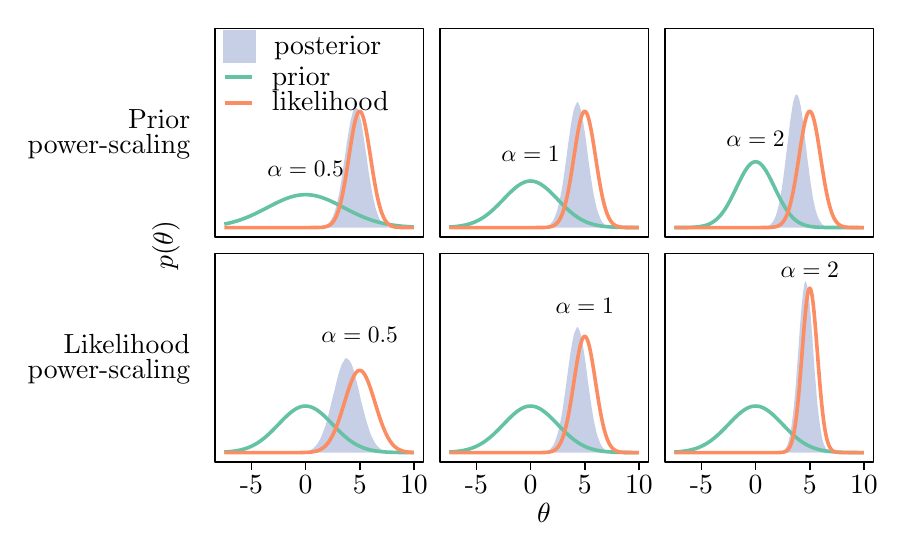
\begin{tikzpicture}[scale=0.85,x=1pt,y=1pt]
\definecolor{fillColor}{RGB}{255,255,255}
\begin{scope}
\definecolor{fillColor}{RGB}{141,160,203}

\path[fill=fillColor,fill opacity=0.50] ( 96.06,210.86) --
	( 96.21,210.86) --
	( 96.37,210.86) --
	( 96.53,210.86) --
	( 96.69,210.86) --
	( 96.85,210.86) --
	( 97.00,210.86) --
	( 97.16,210.86) --
	( 97.32,210.86) --
	( 97.48,210.86) --
	( 97.63,210.86) --
	( 97.79,210.86) --
	( 97.95,210.86) --
	( 98.11,210.86) --
	( 98.27,210.86) --
	( 98.42,210.86) --
	( 98.58,210.86) --
	( 98.74,210.86) --
	( 98.90,210.86) --
	( 99.05,210.86) --
	( 99.21,210.86) --
	( 99.37,210.86) --
	( 99.53,210.86) --
	( 99.68,210.86) --
	( 99.84,210.86) --
	(100.00,210.86) --
	(100.16,210.86) --
	(100.32,210.86) --
	(100.47,210.86) --
	(100.63,210.86) --
	(100.79,210.86) --
	(100.95,210.86) --
	(101.10,210.86) --
	(101.26,210.86) --
	(101.42,210.86) --
	(101.58,210.86) --
	(101.74,210.86) --
	(101.89,210.86) --
	(102.05,210.86) --
	(102.21,210.86) --
	(102.37,210.86) --
	(102.52,210.86) --
	(102.68,210.86) --
	(102.84,210.86) --
	(103.00,210.86) --
	(103.15,210.86) --
	(103.31,210.86) --
	(103.47,210.86) --
	(103.63,210.86) --
	(103.79,210.86) --
	(103.94,210.86) --
	(104.10,210.86) --
	(104.26,210.86) --
	(104.42,210.86) --
	(104.57,210.86) --
	(104.73,210.86) --
	(104.89,210.86) --
	(105.05,210.86) --
	(105.21,210.86) --
	(105.36,210.86) --
	(105.52,210.86) --
	(105.68,210.86) --
	(105.84,210.86) --
	(105.99,210.86) --
	(106.15,210.86) --
	(106.31,210.86) --
	(106.47,210.86) --
	(106.62,210.86) --
	(106.78,210.86) --
	(106.94,210.86) --
	(107.10,210.86) --
	(107.26,210.86) --
	(107.41,210.86) --
	(107.57,210.86) --
	(107.73,210.86) --
	(107.89,210.86) --
	(108.04,210.86) --
	(108.20,210.86) --
	(108.36,210.86) --
	(108.52,210.86) --
	(108.68,210.86) --
	(108.83,210.86) --
	(108.99,210.86) --
	(109.15,210.86) --
	(109.31,210.86) --
	(109.46,210.86) --
	(109.62,210.86) --
	(109.78,210.86) --
	(109.94,210.86) --
	(110.09,210.86) --
	(110.25,210.86) --
	(110.41,210.86) --
	(110.57,210.86) --
	(110.73,210.86) --
	(110.88,210.86) --
	(111.04,210.86) --
	(111.20,210.86) --
	(111.36,210.86) --
	(111.51,210.86) --
	(111.67,210.86) --
	(111.83,210.86) --
	(111.99,210.86) --
	(112.15,210.86) --
	(112.30,210.86) --
	(112.46,210.86) --
	(112.62,210.86) --
	(112.78,210.86) --
	(112.93,210.86) --
	(113.09,210.86) --
	(113.25,210.86) --
	(113.41,210.86) --
	(113.56,210.86) --
	(113.72,210.86) --
	(113.88,210.86) --
	(114.04,210.86) --
	(114.20,210.86) --
	(114.35,210.86) --
	(114.51,210.86) --
	(114.67,210.86) --
	(114.83,210.86) --
	(114.98,210.86) --
	(115.14,210.86) --
	(115.30,210.86) --
	(115.46,210.86) --
	(115.62,210.86) --
	(115.77,210.86) --
	(115.93,210.86) --
	(116.09,210.86) --
	(116.25,210.86) --
	(116.40,210.86) --
	(116.56,210.86) --
	(116.72,210.86) --
	(116.88,210.86) --
	(117.03,210.86) --
	(117.19,210.86) --
	(117.35,210.86) --
	(117.51,210.86) --
	(117.67,210.86) --
	(117.82,210.86) --
	(117.98,210.86) --
	(118.14,210.86) --
	(118.30,210.86) --
	(118.45,210.86) --
	(118.61,210.86) --
	(118.77,210.86) --
	(118.93,210.86) --
	(119.09,210.86) --
	(119.24,210.86) --
	(119.40,210.86) --
	(119.56,210.86) --
	(119.72,210.86) --
	(119.87,210.86) --
	(120.03,210.86) --
	(120.19,210.86) --
	(120.35,210.86) --
	(120.50,210.86) --
	(120.66,210.86) --
	(120.82,210.86) --
	(120.98,210.86) --
	(121.14,210.86) --
	(121.29,210.86) --
	(121.45,210.86) --
	(121.61,210.86) --
	(121.77,210.86) --
	(121.92,210.86) --
	(122.08,210.86) --
	(122.24,210.86) --
	(122.40,210.86) --
	(122.56,210.86) --
	(122.71,210.86) --
	(122.87,210.86) --
	(123.03,210.86) --
	(123.19,210.86) --
	(123.34,210.86) --
	(123.50,210.86) --
	(123.66,210.86) --
	(123.82,210.86) --
	(123.97,210.86) --
	(124.13,210.86) --
	(124.29,210.86) --
	(124.45,210.86) --
	(124.61,210.86) --
	(124.76,210.86) --
	(124.92,210.86) --
	(125.08,210.86) --
	(125.24,210.86) --
	(125.39,210.86) --
	(125.55,210.86) --
	(125.71,210.86) --
	(125.87,210.86) --
	(126.03,210.86) --
	(126.18,210.86) --
	(126.34,210.86) --
	(126.50,210.86) --
	(126.66,210.86) --
	(126.81,210.86) --
	(126.97,210.86) --
	(127.13,210.86) --
	(127.29,210.86) --
	(127.44,210.86) --
	(127.60,210.86) --
	(127.76,210.86) --
	(127.92,210.86) --
	(128.08,210.86) --
	(128.23,210.86) --
	(128.39,210.86) --
	(128.55,210.86) --
	(128.71,210.86) --
	(128.86,210.86) --
	(129.02,210.86) --
	(129.18,210.86) --
	(129.34,210.86) --
	(129.50,210.86) --
	(129.65,210.86) --
	(129.81,210.86) --
	(129.97,210.86) --
	(130.13,210.86) --
	(130.28,210.86) --
	(130.44,210.86) --
	(130.60,210.86) --
	(130.76,210.86) --
	(130.91,210.86) --
	(131.07,210.86) --
	(131.23,210.86) --
	(131.39,210.86) --
	(131.55,210.86) --
	(131.70,210.86) --
	(131.86,210.86) --
	(132.02,210.86) --
	(132.18,210.86) --
	(132.33,210.87) --
	(132.49,210.87) --
	(132.65,210.87) --
	(132.81,210.87) --
	(132.97,210.87) --
	(133.12,210.87) --
	(133.28,210.87) --
	(133.44,210.87) --
	(133.60,210.87) --
	(133.75,210.88) --
	(133.91,210.88) --
	(134.07,210.88) --
	(134.23,210.88) --
	(134.38,210.88) --
	(134.54,210.88) --
	(134.70,210.89) --
	(134.86,210.89) --
	(135.02,210.90) --
	(135.17,210.90) --
	(135.33,210.91) --
	(135.49,210.92) --
	(135.65,210.92) --
	(135.80,210.93) --
	(135.96,210.95) --
	(136.12,210.96) --
	(136.28,210.97) --
	(136.44,210.98) --
	(136.59,211.00) --
	(136.75,211.01) --
	(136.91,211.03) --
	(137.07,211.06) --
	(137.22,211.09) --
	(137.38,211.13) --
	(137.54,211.17) --
	(137.70,211.19) --
	(137.85,211.21) --
	(138.01,211.24) --
	(138.17,211.27) --
	(138.33,211.31) --
	(138.49,211.36) --
	(138.64,211.42) --
	(138.80,211.49) --
	(138.96,211.57) --
	(139.12,211.66) --
	(139.27,211.76) --
	(139.43,211.86) --
	(139.59,211.96) --
	(139.75,212.07) --
	(139.90,212.19) --
	(140.06,212.34) --
	(140.22,212.51) --
	(140.38,212.68) --
	(140.54,212.85) --
	(140.69,213.01) --
	(140.85,213.18) --
	(141.01,213.38) --
	(141.17,213.62) --
	(141.32,213.88) --
	(141.48,214.15) --
	(141.64,214.43) --
	(141.80,214.73) --
	(141.96,215.06) --
	(142.11,215.42) --
	(142.27,215.80) --
	(142.43,216.19) --
	(142.59,216.59) --
	(142.74,216.99) --
	(142.90,217.41) --
	(143.06,217.85) --
	(143.22,218.32) --
	(143.37,218.83) --
	(143.53,219.38) --
	(143.69,219.99) --
	(143.85,220.67) --
	(144.01,221.40) --
	(144.16,222.16) --
	(144.32,222.88) --
	(144.48,223.57) --
	(144.64,224.24) --
	(144.79,224.96) --
	(144.95,225.78) --
	(145.11,226.68) --
	(145.27,227.61) --
	(145.43,228.54) --
	(145.58,229.46) --
	(145.74,230.40) --
	(145.90,231.38) --
	(146.06,232.40) --
	(146.21,233.46) --
	(146.37,234.55) --
	(146.53,235.63) --
	(146.69,236.71) --
	(146.84,237.77) --
	(147.00,238.82) --
	(147.16,239.85) --
	(147.32,240.88) --
	(147.48,241.95) --
	(147.63,243.09) --
	(147.79,244.30) --
	(147.95,245.51) --
	(148.11,246.64) --
	(148.26,247.65) --
	(148.42,248.60) --
	(148.58,249.55) --
	(148.74,250.52) --
	(148.90,251.46) --
	(149.05,252.38) --
	(149.21,253.32) --
	(149.37,254.29) --
	(149.53,255.25) --
	(149.68,256.14) --
	(149.84,256.88) --
	(150.00,257.44) --
	(150.16,257.89) --
	(150.31,258.37) --
	(150.47,259.01) --
	(150.63,259.77) --
	(150.79,260.51) --
	(150.95,261.08) --
	(151.10,261.43) --
	(151.26,261.61) --
	(151.42,261.69) --
	(151.58,261.74) --
	(151.73,261.77) --
	(151.89,261.78) --
	(152.05,261.75) --
	(152.21,261.70) --
	(152.37,261.64) --
	(152.52,261.54) --
	(152.68,261.39) --
	(152.84,261.13) --
	(153.00,260.77) --
	(153.15,260.30) --
	(153.31,259.74) --
	(153.47,259.11) --
	(153.63,258.44) --
	(153.78,257.78) --
	(153.94,257.16) --
	(154.10,256.56) --
	(154.26,255.90) --
	(154.42,255.11) --
	(154.57,254.16) --
	(154.73,253.08) --
	(154.89,251.98) --
	(155.05,250.92) --
	(155.20,249.93) --
	(155.36,248.94) --
	(155.52,247.89) --
	(155.68,246.79) --
	(155.84,245.67) --
	(155.99,244.60) --
	(156.15,243.55) --
	(156.31,242.49) --
	(156.47,241.41) --
	(156.62,240.32) --
	(156.78,239.23) --
	(156.94,238.11) --
	(157.10,236.95) --
	(157.25,235.79) --
	(157.41,234.67) --
	(157.57,233.62) --
	(157.73,232.66) --
	(157.89,231.75) --
	(158.04,230.84) --
	(158.20,229.89) --
	(158.36,228.93) --
	(158.52,227.99) --
	(158.67,227.10) --
	(158.83,226.24) --
	(158.99,225.41) --
	(159.15,224.61) --
	(159.31,223.85) --
	(159.46,223.14) --
	(159.62,222.45) --
	(159.78,221.74) --
	(159.94,221.02) --
	(160.09,220.34) --
	(160.25,219.72) --
	(160.41,219.14) --
	(160.57,218.58) --
	(160.72,218.06) --
	(160.88,217.59) --
	(161.04,217.17) --
	(161.20,216.76) --
	(161.36,216.31) --
	(161.51,215.85) --
	(161.67,215.41) --
	(161.83,215.01) --
	(161.99,214.66) --
	(162.14,214.35) --
	(162.30,214.09) --
	(162.46,213.85) --
	(162.62,213.62) --
	(162.78,213.40) --
	(162.93,213.18) --
	(163.09,212.98) --
	(163.25,212.80) --
	(163.41,212.64) --
	(163.56,212.50) --
	(163.72,212.37) --
	(163.88,212.25) --
	(164.04,212.12) --
	(164.19,212.01) --
	(164.35,211.90) --
	(164.51,211.80) --
	(164.67,211.70) --
	(164.83,211.61) --
	(164.98,211.53) --
	(165.14,211.45) --
	(165.30,211.38) --
	(165.46,211.33) --
	(165.61,211.28) --
	(165.77,211.25) --
	(165.93,211.21) --
	(166.09,211.17) --
	(166.25,211.13) --
	(166.40,211.09) --
	(166.56,211.07) --
	(166.72,211.06) --
	(166.88,211.05) --
	(167.03,211.03) --
	(167.19,211.02) --
	(167.35,211.00) --
	(167.51,210.98) --
	(167.66,210.96) --
	(167.82,210.95) --
	(167.98,210.93) --
	(168.14,210.93) --
	(168.30,210.92) --
	(168.45,210.92) --
	(168.61,210.91) --
	(168.77,210.91) --
	(168.93,210.90) --
	(169.08,210.90) --
	(169.24,210.89) --
	(169.40,210.89) --
	(169.56,210.88) --
	(169.72,210.88) --
	(169.87,210.88) --
	(170.03,210.87) --
	(170.19,210.87) --
	(170.35,210.88) --
	(170.50,210.88) --
	(170.66,210.87) --
	(170.82,210.87) --
	(170.98,210.87) --
	(171.13,210.87) --
	(171.29,210.86) --
	(171.45,210.86) --
	(171.61,210.86) --
	(171.77,210.86) --
	(171.92,210.86) --
	(172.08,210.86) --
	(172.24,210.86) --
	(172.40,210.86) --
	(172.55,210.86) --
	(172.71,210.86) --
	(172.87,210.86) --
	(173.03,210.86) --
	(173.19,210.86) --
	(173.34,210.86) --
	(173.50,210.86) --
	(173.66,210.86) --
	(173.82,210.86) --
	(173.97,210.86) --
	(174.13,210.86) --
	(174.29,210.86) --
	(174.45,210.86) --
	(174.60,210.86) --
	(174.76,210.86) --
	(174.92,210.86) --
	(175.08,210.86) --
	(175.24,210.86) --
	(175.39,210.86) --
	(175.55,210.86) --
	(175.71,210.86) --
	(175.87,210.86) --
	(176.02,210.86) --
	(176.18,210.86) --
	(176.34,210.86) --
	(176.50,210.86) --
	(176.66,210.86) --
	(176.66,210.86) --
	(176.50,210.86) --
	(176.34,210.86) --
	(176.18,210.86) --
	(176.02,210.86) --
	(175.87,210.86) --
	(175.71,210.86) --
	(175.55,210.86) --
	(175.39,210.86) --
	(175.24,210.86) --
	(175.08,210.86) --
	(174.92,210.86) --
	(174.76,210.86) --
	(174.60,210.86) --
	(174.45,210.86) --
	(174.29,210.86) --
	(174.13,210.86) --
	(173.97,210.86) --
	(173.82,210.86) --
	(173.66,210.86) --
	(173.50,210.86) --
	(173.34,210.86) --
	(173.19,210.86) --
	(173.03,210.86) --
	(172.87,210.86) --
	(172.71,210.86) --
	(172.55,210.86) --
	(172.40,210.86) --
	(172.24,210.86) --
	(172.08,210.86) --
	(171.92,210.86) --
	(171.77,210.86) --
	(171.61,210.86) --
	(171.45,210.86) --
	(171.29,210.86) --
	(171.13,210.86) --
	(170.98,210.86) --
	(170.82,210.86) --
	(170.66,210.86) --
	(170.50,210.86) --
	(170.35,210.86) --
	(170.19,210.86) --
	(170.03,210.86) --
	(169.87,210.86) --
	(169.72,210.86) --
	(169.56,210.86) --
	(169.40,210.86) --
	(169.24,210.86) --
	(169.08,210.86) --
	(168.93,210.86) --
	(168.77,210.86) --
	(168.61,210.86) --
	(168.45,210.86) --
	(168.30,210.86) --
	(168.14,210.86) --
	(167.98,210.86) --
	(167.82,210.86) --
	(167.66,210.86) --
	(167.51,210.86) --
	(167.35,210.86) --
	(167.19,210.86) --
	(167.03,210.86) --
	(166.88,210.86) --
	(166.72,210.86) --
	(166.56,210.86) --
	(166.40,210.86) --
	(166.25,210.86) --
	(166.09,210.86) --
	(165.93,210.86) --
	(165.77,210.86) --
	(165.61,210.86) --
	(165.46,210.86) --
	(165.30,210.86) --
	(165.14,210.86) --
	(164.98,210.86) --
	(164.83,210.86) --
	(164.67,210.86) --
	(164.51,210.86) --
	(164.35,210.86) --
	(164.19,210.86) --
	(164.04,210.86) --
	(163.88,210.86) --
	(163.72,210.86) --
	(163.56,210.86) --
	(163.41,210.86) --
	(163.25,210.86) --
	(163.09,210.86) --
	(162.93,210.86) --
	(162.78,210.86) --
	(162.62,210.86) --
	(162.46,210.86) --
	(162.30,210.86) --
	(162.14,210.86) --
	(161.99,210.86) --
	(161.83,210.86) --
	(161.67,210.86) --
	(161.51,210.86) --
	(161.36,210.86) --
	(161.20,210.86) --
	(161.04,210.86) --
	(160.88,210.86) --
	(160.72,210.86) --
	(160.57,210.86) --
	(160.41,210.86) --
	(160.25,210.86) --
	(160.09,210.86) --
	(159.94,210.86) --
	(159.78,210.86) --
	(159.62,210.86) --
	(159.46,210.86) --
	(159.31,210.86) --
	(159.15,210.86) --
	(158.99,210.86) --
	(158.83,210.86) --
	(158.67,210.86) --
	(158.52,210.86) --
	(158.36,210.86) --
	(158.20,210.86) --
	(158.04,210.86) --
	(157.89,210.86) --
	(157.73,210.86) --
	(157.57,210.86) --
	(157.41,210.86) --
	(157.25,210.86) --
	(157.10,210.86) --
	(156.94,210.86) --
	(156.78,210.86) --
	(156.62,210.86) --
	(156.47,210.86) --
	(156.31,210.86) --
	(156.15,210.86) --
	(155.99,210.86) --
	(155.84,210.86) --
	(155.68,210.86) --
	(155.52,210.86) --
	(155.36,210.86) --
	(155.20,210.86) --
	(155.05,210.86) --
	(154.89,210.86) --
	(154.73,210.86) --
	(154.57,210.86) --
	(154.42,210.86) --
	(154.26,210.86) --
	(154.10,210.86) --
	(153.94,210.86) --
	(153.78,210.86) --
	(153.63,210.86) --
	(153.47,210.86) --
	(153.31,210.86) --
	(153.15,210.86) --
	(153.00,210.86) --
	(152.84,210.86) --
	(152.68,210.86) --
	(152.52,210.86) --
	(152.37,210.86) --
	(152.21,210.86) --
	(152.05,210.86) --
	(151.89,210.86) --
	(151.73,210.86) --
	(151.58,210.86) --
	(151.42,210.86) --
	(151.26,210.86) --
	(151.10,210.86) --
	(150.95,210.86) --
	(150.79,210.86) --
	(150.63,210.86) --
	(150.47,210.86) --
	(150.31,210.86) --
	(150.16,210.86) --
	(150.00,210.86) --
	(149.84,210.86) --
	(149.68,210.86) --
	(149.53,210.86) --
	(149.37,210.86) --
	(149.21,210.86) --
	(149.05,210.86) --
	(148.90,210.86) --
	(148.74,210.86) --
	(148.58,210.86) --
	(148.42,210.86) --
	(148.26,210.86) --
	(148.11,210.86) --
	(147.95,210.86) --
	(147.79,210.86) --
	(147.63,210.86) --
	(147.48,210.86) --
	(147.32,210.86) --
	(147.16,210.86) --
	(147.00,210.86) --
	(146.84,210.86) --
	(146.69,210.86) --
	(146.53,210.86) --
	(146.37,210.86) --
	(146.21,210.86) --
	(146.06,210.86) --
	(145.90,210.86) --
	(145.74,210.86) --
	(145.58,210.86) --
	(145.43,210.86) --
	(145.27,210.86) --
	(145.11,210.86) --
	(144.95,210.86) --
	(144.79,210.86) --
	(144.64,210.86) --
	(144.48,210.86) --
	(144.32,210.86) --
	(144.16,210.86) --
	(144.01,210.86) --
	(143.85,210.86) --
	(143.69,210.86) --
	(143.53,210.86) --
	(143.37,210.86) --
	(143.22,210.86) --
	(143.06,210.86) --
	(142.90,210.86) --
	(142.74,210.86) --
	(142.59,210.86) --
	(142.43,210.86) --
	(142.27,210.86) --
	(142.11,210.86) --
	(141.96,210.86) --
	(141.80,210.86) --
	(141.64,210.86) --
	(141.48,210.86) --
	(141.32,210.86) --
	(141.17,210.86) --
	(141.01,210.86) --
	(140.85,210.86) --
	(140.69,210.86) --
	(140.54,210.86) --
	(140.38,210.86) --
	(140.22,210.86) --
	(140.06,210.86) --
	(139.90,210.86) --
	(139.75,210.86) --
	(139.59,210.86) --
	(139.43,210.86) --
	(139.27,210.86) --
	(139.12,210.86) --
	(138.96,210.86) --
	(138.80,210.86) --
	(138.64,210.86) --
	(138.49,210.86) --
	(138.33,210.86) --
	(138.17,210.86) --
	(138.01,210.86) --
	(137.85,210.86) --
	(137.70,210.86) --
	(137.54,210.86) --
	(137.38,210.86) --
	(137.22,210.86) --
	(137.07,210.86) --
	(136.91,210.86) --
	(136.75,210.86) --
	(136.59,210.86) --
	(136.44,210.86) --
	(136.28,210.86) --
	(136.12,210.86) --
	(135.96,210.86) --
	(135.80,210.86) --
	(135.65,210.86) --
	(135.49,210.86) --
	(135.33,210.86) --
	(135.17,210.86) --
	(135.02,210.86) --
	(134.86,210.86) --
	(134.70,210.86) --
	(134.54,210.86) --
	(134.38,210.86) --
	(134.23,210.86) --
	(134.07,210.86) --
	(133.91,210.86) --
	(133.75,210.86) --
	(133.60,210.86) --
	(133.44,210.86) --
	(133.28,210.86) --
	(133.12,210.86) --
	(132.97,210.86) --
	(132.81,210.86) --
	(132.65,210.86) --
	(132.49,210.86) --
	(132.33,210.86) --
	(132.18,210.86) --
	(132.02,210.86) --
	(131.86,210.86) --
	(131.70,210.86) --
	(131.55,210.86) --
	(131.39,210.86) --
	(131.23,210.86) --
	(131.07,210.86) --
	(130.91,210.86) --
	(130.76,210.86) --
	(130.60,210.86) --
	(130.44,210.86) --
	(130.28,210.86) --
	(130.13,210.86) --
	(129.97,210.86) --
	(129.81,210.86) --
	(129.65,210.86) --
	(129.50,210.86) --
	(129.34,210.86) --
	(129.18,210.86) --
	(129.02,210.86) --
	(128.86,210.86) --
	(128.71,210.86) --
	(128.55,210.86) --
	(128.39,210.86) --
	(128.23,210.86) --
	(128.08,210.86) --
	(127.92,210.86) --
	(127.76,210.86) --
	(127.60,210.86) --
	(127.44,210.86) --
	(127.29,210.86) --
	(127.13,210.86) --
	(126.97,210.86) --
	(126.81,210.86) --
	(126.66,210.86) --
	(126.50,210.86) --
	(126.34,210.86) --
	(126.18,210.86) --
	(126.03,210.86) --
	(125.87,210.86) --
	(125.71,210.86) --
	(125.55,210.86) --
	(125.39,210.86) --
	(125.24,210.86) --
	(125.08,210.86) --
	(124.92,210.86) --
	(124.76,210.86) --
	(124.61,210.86) --
	(124.45,210.86) --
	(124.29,210.86) --
	(124.13,210.86) --
	(123.97,210.86) --
	(123.82,210.86) --
	(123.66,210.86) --
	(123.50,210.86) --
	(123.34,210.86) --
	(123.19,210.86) --
	(123.03,210.86) --
	(122.87,210.86) --
	(122.71,210.86) --
	(122.56,210.86) --
	(122.40,210.86) --
	(122.24,210.86) --
	(122.08,210.86) --
	(121.92,210.86) --
	(121.77,210.86) --
	(121.61,210.86) --
	(121.45,210.86) --
	(121.29,210.86) --
	(121.14,210.86) --
	(120.98,210.86) --
	(120.82,210.86) --
	(120.66,210.86) --
	(120.50,210.86) --
	(120.35,210.86) --
	(120.19,210.86) --
	(120.03,210.86) --
	(119.87,210.86) --
	(119.72,210.86) --
	(119.56,210.86) --
	(119.40,210.86) --
	(119.24,210.86) --
	(119.09,210.86) --
	(118.93,210.86) --
	(118.77,210.86) --
	(118.61,210.86) --
	(118.45,210.86) --
	(118.30,210.86) --
	(118.14,210.86) --
	(117.98,210.86) --
	(117.82,210.86) --
	(117.67,210.86) --
	(117.51,210.86) --
	(117.35,210.86) --
	(117.19,210.86) --
	(117.03,210.86) --
	(116.88,210.86) --
	(116.72,210.86) --
	(116.56,210.86) --
	(116.40,210.86) --
	(116.25,210.86) --
	(116.09,210.86) --
	(115.93,210.86) --
	(115.77,210.86) --
	(115.62,210.86) --
	(115.46,210.86) --
	(115.30,210.86) --
	(115.14,210.86) --
	(114.98,210.86) --
	(114.83,210.86) --
	(114.67,210.86) --
	(114.51,210.86) --
	(114.35,210.86) --
	(114.20,210.86) --
	(114.04,210.86) --
	(113.88,210.86) --
	(113.72,210.86) --
	(113.56,210.86) --
	(113.41,210.86) --
	(113.25,210.86) --
	(113.09,210.86) --
	(112.93,210.86) --
	(112.78,210.86) --
	(112.62,210.86) --
	(112.46,210.86) --
	(112.30,210.86) --
	(112.15,210.86) --
	(111.99,210.86) --
	(111.83,210.86) --
	(111.67,210.86) --
	(111.51,210.86) --
	(111.36,210.86) --
	(111.20,210.86) --
	(111.04,210.86) --
	(110.88,210.86) --
	(110.73,210.86) --
	(110.57,210.86) --
	(110.41,210.86) --
	(110.25,210.86) --
	(110.09,210.86) --
	(109.94,210.86) --
	(109.78,210.86) --
	(109.62,210.86) --
	(109.46,210.86) --
	(109.31,210.86) --
	(109.15,210.86) --
	(108.99,210.86) --
	(108.83,210.86) --
	(108.68,210.86) --
	(108.52,210.86) --
	(108.36,210.86) --
	(108.20,210.86) --
	(108.04,210.86) --
	(107.89,210.86) --
	(107.73,210.86) --
	(107.57,210.86) --
	(107.41,210.86) --
	(107.26,210.86) --
	(107.10,210.86) --
	(106.94,210.86) --
	(106.78,210.86) --
	(106.62,210.86) --
	(106.47,210.86) --
	(106.31,210.86) --
	(106.15,210.86) --
	(105.99,210.86) --
	(105.84,210.86) --
	(105.68,210.86) --
	(105.52,210.86) --
	(105.36,210.86) --
	(105.21,210.86) --
	(105.05,210.86) --
	(104.89,210.86) --
	(104.73,210.86) --
	(104.57,210.86) --
	(104.42,210.86) --
	(104.26,210.86) --
	(104.10,210.86) --
	(103.94,210.86) --
	(103.79,210.86) --
	(103.63,210.86) --
	(103.47,210.86) --
	(103.31,210.86) --
	(103.15,210.86) --
	(103.00,210.86) --
	(102.84,210.86) --
	(102.68,210.86) --
	(102.52,210.86) --
	(102.37,210.86) --
	(102.21,210.86) --
	(102.05,210.86) --
	(101.89,210.86) --
	(101.74,210.86) --
	(101.58,210.86) --
	(101.42,210.86) --
	(101.26,210.86) --
	(101.10,210.86) --
	(100.95,210.86) --
	(100.79,210.86) --
	(100.63,210.86) --
	(100.47,210.86) --
	(100.32,210.86) --
	(100.16,210.86) --
	(100.00,210.86) --
	( 99.84,210.86) --
	( 99.68,210.86) --
	( 99.53,210.86) --
	( 99.37,210.86) --
	( 99.21,210.86) --
	( 99.05,210.86) --
	( 98.90,210.86) --
	( 98.74,210.86) --
	( 98.58,210.86) --
	( 98.42,210.86) --
	( 98.27,210.86) --
	( 98.11,210.86) --
	( 97.95,210.86) --
	( 97.79,210.86) --
	( 97.63,210.86) --
	( 97.48,210.86) --
	( 97.32,210.86) --
	( 97.16,210.86) --
	( 97.00,210.86) --
	( 96.85,210.86) --
	( 96.69,210.86) --
	( 96.53,210.86) --
	( 96.37,210.86) --
	( 96.21,210.86) --
	( 96.06,210.86) --
	cycle;

\path[] ( 96.06,210.86) --
	( 96.21,210.86) --
	( 96.37,210.86) --
	( 96.53,210.86) --
	( 96.69,210.86) --
	( 96.85,210.86) --
	( 97.00,210.86) --
	( 97.16,210.86) --
	( 97.32,210.86) --
	( 97.48,210.86) --
	( 97.63,210.86) --
	( 97.79,210.86) --
	( 97.95,210.86) --
	( 98.11,210.86) --
	( 98.27,210.86) --
	( 98.42,210.86) --
	( 98.58,210.86) --
	( 98.74,210.86) --
	( 98.90,210.86) --
	( 99.05,210.86) --
	( 99.21,210.86) --
	( 99.37,210.86) --
	( 99.53,210.86) --
	( 99.68,210.86) --
	( 99.84,210.86) --
	(100.00,210.86) --
	(100.16,210.86) --
	(100.32,210.86) --
	(100.47,210.86) --
	(100.63,210.86) --
	(100.79,210.86) --
	(100.95,210.86) --
	(101.10,210.86) --
	(101.26,210.86) --
	(101.42,210.86) --
	(101.58,210.86) --
	(101.74,210.86) --
	(101.89,210.86) --
	(102.05,210.86) --
	(102.21,210.86) --
	(102.37,210.86) --
	(102.52,210.86) --
	(102.68,210.86) --
	(102.84,210.86) --
	(103.00,210.86) --
	(103.15,210.86) --
	(103.31,210.86) --
	(103.47,210.86) --
	(103.63,210.86) --
	(103.79,210.86) --
	(103.94,210.86) --
	(104.10,210.86) --
	(104.26,210.86) --
	(104.42,210.86) --
	(104.57,210.86) --
	(104.73,210.86) --
	(104.89,210.86) --
	(105.05,210.86) --
	(105.21,210.86) --
	(105.36,210.86) --
	(105.52,210.86) --
	(105.68,210.86) --
	(105.84,210.86) --
	(105.99,210.86) --
	(106.15,210.86) --
	(106.31,210.86) --
	(106.47,210.86) --
	(106.62,210.86) --
	(106.78,210.86) --
	(106.94,210.86) --
	(107.10,210.86) --
	(107.26,210.86) --
	(107.41,210.86) --
	(107.57,210.86) --
	(107.73,210.86) --
	(107.89,210.86) --
	(108.04,210.86) --
	(108.20,210.86) --
	(108.36,210.86) --
	(108.52,210.86) --
	(108.68,210.86) --
	(108.83,210.86) --
	(108.99,210.86) --
	(109.15,210.86) --
	(109.31,210.86) --
	(109.46,210.86) --
	(109.62,210.86) --
	(109.78,210.86) --
	(109.94,210.86) --
	(110.09,210.86) --
	(110.25,210.86) --
	(110.41,210.86) --
	(110.57,210.86) --
	(110.73,210.86) --
	(110.88,210.86) --
	(111.04,210.86) --
	(111.20,210.86) --
	(111.36,210.86) --
	(111.51,210.86) --
	(111.67,210.86) --
	(111.83,210.86) --
	(111.99,210.86) --
	(112.15,210.86) --
	(112.30,210.86) --
	(112.46,210.86) --
	(112.62,210.86) --
	(112.78,210.86) --
	(112.93,210.86) --
	(113.09,210.86) --
	(113.25,210.86) --
	(113.41,210.86) --
	(113.56,210.86) --
	(113.72,210.86) --
	(113.88,210.86) --
	(114.04,210.86) --
	(114.20,210.86) --
	(114.35,210.86) --
	(114.51,210.86) --
	(114.67,210.86) --
	(114.83,210.86) --
	(114.98,210.86) --
	(115.14,210.86) --
	(115.30,210.86) --
	(115.46,210.86) --
	(115.62,210.86) --
	(115.77,210.86) --
	(115.93,210.86) --
	(116.09,210.86) --
	(116.25,210.86) --
	(116.40,210.86) --
	(116.56,210.86) --
	(116.72,210.86) --
	(116.88,210.86) --
	(117.03,210.86) --
	(117.19,210.86) --
	(117.35,210.86) --
	(117.51,210.86) --
	(117.67,210.86) --
	(117.82,210.86) --
	(117.98,210.86) --
	(118.14,210.86) --
	(118.30,210.86) --
	(118.45,210.86) --
	(118.61,210.86) --
	(118.77,210.86) --
	(118.93,210.86) --
	(119.09,210.86) --
	(119.24,210.86) --
	(119.40,210.86) --
	(119.56,210.86) --
	(119.72,210.86) --
	(119.87,210.86) --
	(120.03,210.86) --
	(120.19,210.86) --
	(120.35,210.86) --
	(120.50,210.86) --
	(120.66,210.86) --
	(120.82,210.86) --
	(120.98,210.86) --
	(121.14,210.86) --
	(121.29,210.86) --
	(121.45,210.86) --
	(121.61,210.86) --
	(121.77,210.86) --
	(121.92,210.86) --
	(122.08,210.86) --
	(122.24,210.86) --
	(122.40,210.86) --
	(122.56,210.86) --
	(122.71,210.86) --
	(122.87,210.86) --
	(123.03,210.86) --
	(123.19,210.86) --
	(123.34,210.86) --
	(123.50,210.86) --
	(123.66,210.86) --
	(123.82,210.86) --
	(123.97,210.86) --
	(124.13,210.86) --
	(124.29,210.86) --
	(124.45,210.86) --
	(124.61,210.86) --
	(124.76,210.86) --
	(124.92,210.86) --
	(125.08,210.86) --
	(125.24,210.86) --
	(125.39,210.86) --
	(125.55,210.86) --
	(125.71,210.86) --
	(125.87,210.86) --
	(126.03,210.86) --
	(126.18,210.86) --
	(126.34,210.86) --
	(126.50,210.86) --
	(126.66,210.86) --
	(126.81,210.86) --
	(126.97,210.86) --
	(127.13,210.86) --
	(127.29,210.86) --
	(127.44,210.86) --
	(127.60,210.86) --
	(127.76,210.86) --
	(127.92,210.86) --
	(128.08,210.86) --
	(128.23,210.86) --
	(128.39,210.86) --
	(128.55,210.86) --
	(128.71,210.86) --
	(128.86,210.86) --
	(129.02,210.86) --
	(129.18,210.86) --
	(129.34,210.86) --
	(129.50,210.86) --
	(129.65,210.86) --
	(129.81,210.86) --
	(129.97,210.86) --
	(130.13,210.86) --
	(130.28,210.86) --
	(130.44,210.86) --
	(130.60,210.86) --
	(130.76,210.86) --
	(130.91,210.86) --
	(131.07,210.86) --
	(131.23,210.86) --
	(131.39,210.86) --
	(131.55,210.86) --
	(131.70,210.86) --
	(131.86,210.86) --
	(132.02,210.86) --
	(132.18,210.86) --
	(132.33,210.87) --
	(132.49,210.87) --
	(132.65,210.87) --
	(132.81,210.87) --
	(132.97,210.87) --
	(133.12,210.87) --
	(133.28,210.87) --
	(133.44,210.87) --
	(133.60,210.87) --
	(133.75,210.88) --
	(133.91,210.88) --
	(134.07,210.88) --
	(134.23,210.88) --
	(134.38,210.88) --
	(134.54,210.88) --
	(134.70,210.89) --
	(134.86,210.89) --
	(135.02,210.90) --
	(135.17,210.90) --
	(135.33,210.91) --
	(135.49,210.92) --
	(135.65,210.92) --
	(135.80,210.93) --
	(135.96,210.95) --
	(136.12,210.96) --
	(136.28,210.97) --
	(136.44,210.98) --
	(136.59,211.00) --
	(136.75,211.01) --
	(136.91,211.03) --
	(137.07,211.06) --
	(137.22,211.09) --
	(137.38,211.13) --
	(137.54,211.17) --
	(137.70,211.19) --
	(137.85,211.21) --
	(138.01,211.24) --
	(138.17,211.27) --
	(138.33,211.31) --
	(138.49,211.36) --
	(138.64,211.42) --
	(138.80,211.49) --
	(138.96,211.57) --
	(139.12,211.66) --
	(139.27,211.76) --
	(139.43,211.86) --
	(139.59,211.96) --
	(139.75,212.07) --
	(139.90,212.19) --
	(140.06,212.34) --
	(140.22,212.51) --
	(140.38,212.68) --
	(140.54,212.85) --
	(140.69,213.01) --
	(140.85,213.18) --
	(141.01,213.38) --
	(141.17,213.62) --
	(141.32,213.88) --
	(141.48,214.15) --
	(141.64,214.43) --
	(141.80,214.73) --
	(141.96,215.06) --
	(142.11,215.42) --
	(142.27,215.80) --
	(142.43,216.19) --
	(142.59,216.59) --
	(142.74,216.99) --
	(142.90,217.41) --
	(143.06,217.85) --
	(143.22,218.32) --
	(143.37,218.83) --
	(143.53,219.38) --
	(143.69,219.99) --
	(143.85,220.67) --
	(144.01,221.40) --
	(144.16,222.16) --
	(144.32,222.88) --
	(144.48,223.57) --
	(144.64,224.24) --
	(144.79,224.96) --
	(144.95,225.78) --
	(145.11,226.68) --
	(145.27,227.61) --
	(145.43,228.54) --
	(145.58,229.46) --
	(145.74,230.40) --
	(145.90,231.38) --
	(146.06,232.40) --
	(146.21,233.46) --
	(146.37,234.55) --
	(146.53,235.63) --
	(146.69,236.71) --
	(146.84,237.77) --
	(147.00,238.82) --
	(147.16,239.85) --
	(147.32,240.88) --
	(147.48,241.95) --
	(147.63,243.09) --
	(147.79,244.30) --
	(147.95,245.51) --
	(148.11,246.64) --
	(148.26,247.65) --
	(148.42,248.60) --
	(148.58,249.55) --
	(148.74,250.52) --
	(148.90,251.46) --
	(149.05,252.38) --
	(149.21,253.32) --
	(149.37,254.29) --
	(149.53,255.25) --
	(149.68,256.14) --
	(149.84,256.88) --
	(150.00,257.44) --
	(150.16,257.89) --
	(150.31,258.37) --
	(150.47,259.01) --
	(150.63,259.77) --
	(150.79,260.51) --
	(150.95,261.08) --
	(151.10,261.43) --
	(151.26,261.61) --
	(151.42,261.69) --
	(151.58,261.74) --
	(151.73,261.77) --
	(151.89,261.78) --
	(152.05,261.75) --
	(152.21,261.70) --
	(152.37,261.64) --
	(152.52,261.54) --
	(152.68,261.39) --
	(152.84,261.13) --
	(153.00,260.77) --
	(153.15,260.30) --
	(153.31,259.74) --
	(153.47,259.11) --
	(153.63,258.44) --
	(153.78,257.78) --
	(153.94,257.16) --
	(154.10,256.56) --
	(154.26,255.90) --
	(154.42,255.11) --
	(154.57,254.16) --
	(154.73,253.08) --
	(154.89,251.98) --
	(155.05,250.92) --
	(155.20,249.93) --
	(155.36,248.94) --
	(155.52,247.89) --
	(155.68,246.79) --
	(155.84,245.67) --
	(155.99,244.60) --
	(156.15,243.55) --
	(156.31,242.49) --
	(156.47,241.41) --
	(156.62,240.32) --
	(156.78,239.23) --
	(156.94,238.11) --
	(157.10,236.95) --
	(157.25,235.79) --
	(157.41,234.67) --
	(157.57,233.62) --
	(157.73,232.66) --
	(157.89,231.75) --
	(158.04,230.84) --
	(158.20,229.89) --
	(158.36,228.93) --
	(158.52,227.99) --
	(158.67,227.10) --
	(158.83,226.24) --
	(158.99,225.41) --
	(159.15,224.61) --
	(159.31,223.85) --
	(159.46,223.14) --
	(159.62,222.45) --
	(159.78,221.74) --
	(159.94,221.02) --
	(160.09,220.34) --
	(160.25,219.72) --
	(160.41,219.14) --
	(160.57,218.58) --
	(160.72,218.06) --
	(160.88,217.59) --
	(161.04,217.17) --
	(161.20,216.76) --
	(161.36,216.31) --
	(161.51,215.85) --
	(161.67,215.41) --
	(161.83,215.01) --
	(161.99,214.66) --
	(162.14,214.35) --
	(162.30,214.09) --
	(162.46,213.85) --
	(162.62,213.62) --
	(162.78,213.40) --
	(162.93,213.18) --
	(163.09,212.98) --
	(163.25,212.80) --
	(163.41,212.64) --
	(163.56,212.50) --
	(163.72,212.37) --
	(163.88,212.25) --
	(164.04,212.12) --
	(164.19,212.01) --
	(164.35,211.90) --
	(164.51,211.80) --
	(164.67,211.70) --
	(164.83,211.61) --
	(164.98,211.53) --
	(165.14,211.45) --
	(165.30,211.38) --
	(165.46,211.33) --
	(165.61,211.28) --
	(165.77,211.25) --
	(165.93,211.21) --
	(166.09,211.17) --
	(166.25,211.13) --
	(166.40,211.09) --
	(166.56,211.07) --
	(166.72,211.06) --
	(166.88,211.05) --
	(167.03,211.03) --
	(167.19,211.02) --
	(167.35,211.00) --
	(167.51,210.98) --
	(167.66,210.96) --
	(167.82,210.95) --
	(167.98,210.93) --
	(168.14,210.93) --
	(168.30,210.92) --
	(168.45,210.92) --
	(168.61,210.91) --
	(168.77,210.91) --
	(168.93,210.90) --
	(169.08,210.90) --
	(169.24,210.89) --
	(169.40,210.89) --
	(169.56,210.88) --
	(169.72,210.88) --
	(169.87,210.88) --
	(170.03,210.87) --
	(170.19,210.87) --
	(170.35,210.88) --
	(170.50,210.88) --
	(170.66,210.87) --
	(170.82,210.87) --
	(170.98,210.87) --
	(171.13,210.87) --
	(171.29,210.86) --
	(171.45,210.86) --
	(171.61,210.86) --
	(171.77,210.86) --
	(171.92,210.86) --
	(172.08,210.86) --
	(172.24,210.86) --
	(172.40,210.86) --
	(172.55,210.86) --
	(172.71,210.86) --
	(172.87,210.86) --
	(173.03,210.86) --
	(173.19,210.86) --
	(173.34,210.86) --
	(173.50,210.86) --
	(173.66,210.86) --
	(173.82,210.86) --
	(173.97,210.86) --
	(174.13,210.86) --
	(174.29,210.86) --
	(174.45,210.86) --
	(174.60,210.86) --
	(174.76,210.86) --
	(174.92,210.86) --
	(175.08,210.86) --
	(175.24,210.86) --
	(175.39,210.86) --
	(175.55,210.86) --
	(175.71,210.86) --
	(175.87,210.86) --
	(176.02,210.86) --
	(176.18,210.86) --
	(176.34,210.86) --
	(176.50,210.86) --
	(176.66,210.86);
\definecolor{drawColor}{RGB}{102,194,165}

\path[draw=drawColor,line width= 1.3pt,line join=round] ( 96.06,212.34) --
	( 96.52,212.43) --
	( 96.98,212.53) --
	( 97.44,212.63) --
	( 97.90,212.73) --
	( 98.36,212.84) --
	( 98.82,212.95) --
	( 99.28,213.07) --
	( 99.74,213.19) --
	(100.20,213.32) --
	(100.66,213.45) --
	(101.12,213.58) --
	(101.58,213.73) --
	(102.04,213.87) --
	(102.51,214.02) --
	(102.97,214.18) --
	(103.43,214.34) --
	(103.89,214.51) --
	(104.35,214.68) --
	(104.81,214.85) --
	(105.27,215.04) --
	(105.73,215.22) --
	(106.19,215.41) --
	(106.65,215.61) --
	(107.11,215.81) --
	(107.57,216.01) --
	(108.03,216.22) --
	(108.49,216.43) --
	(108.95,216.64) --
	(109.41,216.86) --
	(109.87,217.08) --
	(110.33,217.31) --
	(110.80,217.54) --
	(111.26,217.77) --
	(111.72,218.00) --
	(112.18,218.24) --
	(112.64,218.47) --
	(113.10,218.71) --
	(113.56,218.95) --
	(114.02,219.19) --
	(114.48,219.43) --
	(114.94,219.67) --
	(115.40,219.91) --
	(115.86,220.15) --
	(116.32,220.38) --
	(116.78,220.62) --
	(117.24,220.85) --
	(117.70,221.08) --
	(118.16,221.31) --
	(118.62,221.53) --
	(119.09,221.75) --
	(119.55,221.97) --
	(120.01,222.18) --
	(120.47,222.39) --
	(120.93,222.59) --
	(121.39,222.78) --
	(121.85,222.97) --
	(122.31,223.15) --
	(122.77,223.32) --
	(123.23,223.49) --
	(123.69,223.65) --
	(124.15,223.80) --
	(124.61,223.94) --
	(125.07,224.07) --
	(125.53,224.19) --
	(125.99,224.30) --
	(126.45,224.40) --
	(126.91,224.50) --
	(127.38,224.58) --
	(127.84,224.65) --
	(128.30,224.71) --
	(128.76,224.76) --
	(129.22,224.80) --
	(129.68,224.83) --
	(130.14,224.85) --
	(130.60,224.85) --
	(131.06,224.85) --
	(131.52,224.83) --
	(131.98,224.80) --
	(132.44,224.76) --
	(132.90,224.71) --
	(133.36,224.65) --
	(133.82,224.58) --
	(134.28,224.50) --
	(134.74,224.40) --
	(135.20,224.30) --
	(135.67,224.19) --
	(136.13,224.07) --
	(136.59,223.94) --
	(137.05,223.80) --
	(137.51,223.65) --
	(137.97,223.49) --
	(138.43,223.32) --
	(138.89,223.15) --
	(139.35,222.97) --
	(139.81,222.78) --
	(140.27,222.59) --
	(140.73,222.39) --
	(141.19,222.18) --
	(141.65,221.97) --
	(142.11,221.75) --
	(142.57,221.53) --
	(143.03,221.31) --
	(143.49,221.08) --
	(143.96,220.85) --
	(144.42,220.62) --
	(144.88,220.38) --
	(145.34,220.15) --
	(145.80,219.91) --
	(146.26,219.67) --
	(146.72,219.43) --
	(147.18,219.19) --
	(147.64,218.95) --
	(148.10,218.71) --
	(148.56,218.47) --
	(149.02,218.24) --
	(149.48,218.00) --
	(149.94,217.77) --
	(150.40,217.54) --
	(150.86,217.31) --
	(151.32,217.08) --
	(151.78,216.86) --
	(152.25,216.64) --
	(152.71,216.43) --
	(153.17,216.22) --
	(153.63,216.01) --
	(154.09,215.81) --
	(154.55,215.61) --
	(155.01,215.41) --
	(155.47,215.22) --
	(155.93,215.04) --
	(156.39,214.85) --
	(156.85,214.68) --
	(157.31,214.51) --
	(157.77,214.34) --
	(158.23,214.18) --
	(158.69,214.02) --
	(159.15,213.87) --
	(159.61,213.73) --
	(160.07,213.58) --
	(160.54,213.45) --
	(161.00,213.32) --
	(161.46,213.19) --
	(161.92,213.07) --
	(162.38,212.95) --
	(162.84,212.84) --
	(163.30,212.73) --
	(163.76,212.63) --
	(164.22,212.53) --
	(164.68,212.43) --
	(165.14,212.34) --
	(165.60,212.26) --
	(166.06,212.17) --
	(166.52,212.09) --
	(166.98,212.02) --
	(167.44,211.95) --
	(167.90,211.88) --
	(168.36,211.82) --
	(168.83,211.76) --
	(169.29,211.70) --
	(169.75,211.64) --
	(170.21,211.59) --
	(170.67,211.54) --
	(171.13,211.50) --
	(171.59,211.46) --
	(172.05,211.41) --
	(172.51,211.38) --
	(172.97,211.34) --
	(173.43,211.31) --
	(173.89,211.27) --
	(174.35,211.25) --
	(174.81,211.22) --
	(175.27,211.19) --
	(175.73,211.17) --
	(176.19,211.14) --
	(176.66,211.12);
\definecolor{drawColor}{RGB}{252,141,98}

\path[draw=drawColor,line width= 1.3pt,line join=round] ( 96.06,210.86) --
	( 96.52,210.86) --
	( 96.98,210.86) --
	( 97.44,210.86) --
	( 97.90,210.86) --
	( 98.36,210.86) --
	( 98.82,210.86) --
	( 99.28,210.86) --
	( 99.74,210.86) --
	(100.20,210.86) --
	(100.66,210.86) --
	(101.12,210.86) --
	(101.58,210.86) --
	(102.04,210.86) --
	(102.51,210.86) --
	(102.97,210.86) --
	(103.43,210.86) --
	(103.89,210.86) --
	(104.35,210.86) --
	(104.81,210.86) --
	(105.27,210.86) --
	(105.73,210.86) --
	(106.19,210.86) --
	(106.65,210.86) --
	(107.11,210.86) --
	(107.57,210.86) --
	(108.03,210.86) --
	(108.49,210.86) --
	(108.95,210.86) --
	(109.41,210.86) --
	(109.87,210.86) --
	(110.33,210.86) --
	(110.80,210.86) --
	(111.26,210.86) --
	(111.72,210.86) --
	(112.18,210.86) --
	(112.64,210.86) --
	(113.10,210.86) --
	(113.56,210.86) --
	(114.02,210.86) --
	(114.48,210.86) --
	(114.94,210.86) --
	(115.40,210.86) --
	(115.86,210.86) --
	(116.32,210.86) --
	(116.78,210.86) --
	(117.24,210.86) --
	(117.70,210.86) --
	(118.16,210.86) --
	(118.62,210.86) --
	(119.09,210.86) --
	(119.55,210.86) --
	(120.01,210.86) --
	(120.47,210.86) --
	(120.93,210.86) --
	(121.39,210.86) --
	(121.85,210.86) --
	(122.31,210.86) --
	(122.77,210.86) --
	(123.23,210.86) --
	(123.69,210.86) --
	(124.15,210.86) --
	(124.61,210.86) --
	(125.07,210.86) --
	(125.53,210.86) --
	(125.99,210.86) --
	(126.45,210.86) --
	(126.91,210.86) --
	(127.38,210.86) --
	(127.84,210.86) --
	(128.30,210.86) --
	(128.76,210.86) --
	(129.22,210.86) --
	(129.68,210.86) --
	(130.14,210.86) --
	(130.60,210.86) --
	(131.06,210.86) --
	(131.52,210.86) --
	(131.98,210.86) --
	(132.44,210.86) --
	(132.90,210.87) --
	(133.36,210.87) --
	(133.82,210.87) --
	(134.28,210.87) --
	(134.74,210.87) --
	(135.20,210.88) --
	(135.67,210.89) --
	(136.13,210.90) --
	(136.59,210.92) --
	(137.05,210.94) --
	(137.51,210.97) --
	(137.97,211.02) --
	(138.43,211.08) --
	(138.89,211.16) --
	(139.35,211.28) --
	(139.81,211.42) --
	(140.27,211.61) --
	(140.73,211.86) --
	(141.19,212.17) --
	(141.65,212.56) --
	(142.11,213.05) --
	(142.57,213.65) --
	(143.03,214.39) --
	(143.49,215.28) --
	(143.96,216.33) --
	(144.42,217.57) --
	(144.88,219.01) --
	(145.34,220.66) --
	(145.80,222.53) --
	(146.26,224.62) --
	(146.72,226.92) --
	(147.18,229.42) --
	(147.64,232.10) --
	(148.10,234.93) --
	(148.56,237.86) --
	(149.02,240.85) --
	(149.48,243.84) --
	(149.94,246.77) --
	(150.40,249.56) --
	(150.86,252.17) --
	(151.32,254.50) --
	(151.78,256.51) --
	(152.25,258.14) --
	(152.71,259.34) --
	(153.17,260.07) --
	(153.63,260.32) --
	(154.09,260.07) --
	(154.55,259.34) --
	(155.01,258.14) --
	(155.47,256.51) --
	(155.93,254.50) --
	(156.39,252.17) --
	(156.85,249.56) --
	(157.31,246.77) --
	(157.77,243.84) --
	(158.23,240.85) --
	(158.69,237.86) --
	(159.15,234.93) --
	(159.61,232.10) --
	(160.07,229.42) --
	(160.54,226.92) --
	(161.00,224.62) --
	(161.46,222.53) --
	(161.92,220.66) --
	(162.38,219.01) --
	(162.84,217.57) --
	(163.30,216.33) --
	(163.76,215.28) --
	(164.22,214.39) --
	(164.68,213.65) --
	(165.14,213.05) --
	(165.60,212.56) --
	(166.06,212.17) --
	(166.52,211.86) --
	(166.98,211.61) --
	(167.44,211.42) --
	(167.90,211.28) --
	(168.36,211.16) --
	(168.83,211.08) --
	(169.29,211.02) --
	(169.75,210.97) --
	(170.21,210.94) --
	(170.67,210.92) --
	(171.13,210.90) --
	(171.59,210.89) --
	(172.05,210.88) --
	(172.51,210.87) --
	(172.97,210.87) --
	(173.43,210.87) --
	(173.89,210.87) --
	(174.35,210.87) --
	(174.81,210.86) --
	(175.27,210.86) --
	(175.73,210.86) --
	(176.19,210.86) --
	(176.66,210.86);
\definecolor{drawColor}{RGB}{0,0,0}

\node[text=drawColor,anchor=base,inner sep=0pt, outer sep=0pt, scale=  0.85] at (130.60,232.72) {$\alpha = 0.5$};

\path[draw=drawColor,line width= 0.6pt,line join=round,line cap=round] ( 92.03,206.83) rectangle (180.68,295.49);
\end{scope}
\begin{scope}
\definecolor{fillColor}{RGB}{141,160,203}

\path[fill=fillColor,fill opacity=0.50] ( 96.06,115.21) --
	( 96.21,115.21) --
	( 96.37,115.21) --
	( 96.53,115.21) --
	( 96.69,115.21) --
	( 96.85,115.21) --
	( 97.00,115.21) --
	( 97.16,115.21) --
	( 97.32,115.21) --
	( 97.48,115.21) --
	( 97.63,115.21) --
	( 97.79,115.21) --
	( 97.95,115.21) --
	( 98.11,115.21) --
	( 98.27,115.21) --
	( 98.42,115.21) --
	( 98.58,115.21) --
	( 98.74,115.21) --
	( 98.90,115.21) --
	( 99.05,115.21) --
	( 99.21,115.21) --
	( 99.37,115.21) --
	( 99.53,115.21) --
	( 99.68,115.21) --
	( 99.84,115.21) --
	(100.00,115.21) --
	(100.16,115.21) --
	(100.32,115.21) --
	(100.47,115.21) --
	(100.63,115.21) --
	(100.79,115.21) --
	(100.95,115.21) --
	(101.10,115.21) --
	(101.26,115.21) --
	(101.42,115.21) --
	(101.58,115.21) --
	(101.74,115.21) --
	(101.89,115.21) --
	(102.05,115.21) --
	(102.21,115.21) --
	(102.37,115.21) --
	(102.52,115.21) --
	(102.68,115.21) --
	(102.84,115.21) --
	(103.00,115.21) --
	(103.15,115.21) --
	(103.31,115.21) --
	(103.47,115.21) --
	(103.63,115.21) --
	(103.79,115.21) --
	(103.94,115.21) --
	(104.10,115.21) --
	(104.26,115.21) --
	(104.42,115.21) --
	(104.57,115.21) --
	(104.73,115.21) --
	(104.89,115.21) --
	(105.05,115.21) --
	(105.21,115.21) --
	(105.36,115.21) --
	(105.52,115.21) --
	(105.68,115.21) --
	(105.84,115.21) --
	(105.99,115.21) --
	(106.15,115.21) --
	(106.31,115.21) --
	(106.47,115.21) --
	(106.62,115.21) --
	(106.78,115.21) --
	(106.94,115.21) --
	(107.10,115.21) --
	(107.26,115.21) --
	(107.41,115.21) --
	(107.57,115.21) --
	(107.73,115.21) --
	(107.89,115.21) --
	(108.04,115.21) --
	(108.20,115.21) --
	(108.36,115.21) --
	(108.52,115.21) --
	(108.68,115.21) --
	(108.83,115.21) --
	(108.99,115.21) --
	(109.15,115.21) --
	(109.31,115.21) --
	(109.46,115.21) --
	(109.62,115.21) --
	(109.78,115.21) --
	(109.94,115.21) --
	(110.09,115.21) --
	(110.25,115.21) --
	(110.41,115.21) --
	(110.57,115.21) --
	(110.73,115.21) --
	(110.88,115.21) --
	(111.04,115.21) --
	(111.20,115.21) --
	(111.36,115.21) --
	(111.51,115.21) --
	(111.67,115.21) --
	(111.83,115.21) --
	(111.99,115.21) --
	(112.15,115.21) --
	(112.30,115.21) --
	(112.46,115.21) --
	(112.62,115.21) --
	(112.78,115.21) --
	(112.93,115.21) --
	(113.09,115.21) --
	(113.25,115.21) --
	(113.41,115.21) --
	(113.56,115.21) --
	(113.72,115.21) --
	(113.88,115.21) --
	(114.04,115.21) --
	(114.20,115.21) --
	(114.35,115.21) --
	(114.51,115.21) --
	(114.67,115.21) --
	(114.83,115.21) --
	(114.98,115.21) --
	(115.14,115.21) --
	(115.30,115.21) --
	(115.46,115.21) --
	(115.62,115.21) --
	(115.77,115.21) --
	(115.93,115.21) --
	(116.09,115.21) --
	(116.25,115.21) --
	(116.40,115.21) --
	(116.56,115.21) --
	(116.72,115.21) --
	(116.88,115.21) --
	(117.03,115.21) --
	(117.19,115.21) --
	(117.35,115.21) --
	(117.51,115.21) --
	(117.67,115.21) --
	(117.82,115.21) --
	(117.98,115.21) --
	(118.14,115.21) --
	(118.30,115.21) --
	(118.45,115.21) --
	(118.61,115.21) --
	(118.77,115.21) --
	(118.93,115.21) --
	(119.09,115.21) --
	(119.24,115.21) --
	(119.40,115.21) --
	(119.56,115.21) --
	(119.72,115.21) --
	(119.87,115.21) --
	(120.03,115.21) --
	(120.19,115.21) --
	(120.35,115.21) --
	(120.50,115.21) --
	(120.66,115.21) --
	(120.82,115.21) --
	(120.98,115.21) --
	(121.14,115.21) --
	(121.29,115.21) --
	(121.45,115.21) --
	(121.61,115.21) --
	(121.77,115.21) --
	(121.92,115.21) --
	(122.08,115.21) --
	(122.24,115.21) --
	(122.40,115.21) --
	(122.56,115.21) --
	(122.71,115.21) --
	(122.87,115.21) --
	(123.03,115.21) --
	(123.19,115.21) --
	(123.34,115.21) --
	(123.50,115.21) --
	(123.66,115.21) --
	(123.82,115.21) --
	(123.97,115.21) --
	(124.13,115.21) --
	(124.29,115.21) --
	(124.45,115.21) --
	(124.61,115.21) --
	(124.76,115.22) --
	(124.92,115.22) --
	(125.08,115.22) --
	(125.24,115.22) --
	(125.39,115.22) --
	(125.55,115.22) --
	(125.71,115.23) --
	(125.87,115.23) --
	(126.03,115.23) --
	(126.18,115.23) --
	(126.34,115.24) --
	(126.50,115.24) --
	(126.66,115.24) --
	(126.81,115.25) --
	(126.97,115.25) --
	(127.13,115.26) --
	(127.29,115.26) --
	(127.44,115.27) --
	(127.60,115.27) --
	(127.76,115.28) --
	(127.92,115.29) --
	(128.08,115.30) --
	(128.23,115.31) --
	(128.39,115.32) --
	(128.55,115.33) --
	(128.71,115.33) --
	(128.86,115.34) --
	(129.02,115.35) --
	(129.18,115.36) --
	(129.34,115.38) --
	(129.50,115.40) --
	(129.65,115.42) --
	(129.81,115.44) --
	(129.97,115.47) --
	(130.13,115.50) --
	(130.28,115.53) --
	(130.44,115.55) --
	(130.60,115.58) --
	(130.76,115.61) --
	(130.91,115.65) --
	(131.07,115.69) --
	(131.23,115.74) --
	(131.39,115.79) --
	(131.55,115.83) --
	(131.70,115.87) --
	(131.86,115.92) --
	(132.02,115.97) --
	(132.18,116.03) --
	(132.33,116.10) --
	(132.49,116.17) --
	(132.65,116.25) --
	(132.81,116.32) --
	(132.97,116.40) --
	(133.12,116.49) --
	(133.28,116.59) --
	(133.44,116.70) --
	(133.60,116.82) --
	(133.75,116.94) --
	(133.91,117.06) --
	(134.07,117.18) --
	(134.23,117.32) --
	(134.38,117.48) --
	(134.54,117.65) --
	(134.70,117.82) --
	(134.86,118.00) --
	(135.02,118.18) --
	(135.17,118.37) --
	(135.33,118.57) --
	(135.49,118.78) --
	(135.65,118.99) --
	(135.80,119.22) --
	(135.96,119.46) --
	(136.12,119.73) --
	(136.28,120.01) --
	(136.44,120.29) --
	(136.59,120.58) --
	(136.75,120.87) --
	(136.91,121.18) --
	(137.07,121.50) --
	(137.22,121.85) --
	(137.38,122.22) --
	(137.54,122.60) --
	(137.70,123.01) --
	(137.85,123.45) --
	(138.01,123.89) --
	(138.17,124.34) --
	(138.33,124.77) --
	(138.49,125.18) --
	(138.64,125.58) --
	(138.80,125.98) --
	(138.96,126.42) --
	(139.12,126.90) --
	(139.27,127.42) --
	(139.43,127.98) --
	(139.59,128.56) --
	(139.75,129.14) --
	(139.90,129.72) --
	(140.06,130.29) --
	(140.22,130.88) --
	(140.38,131.48) --
	(140.54,132.09) --
	(140.69,132.73) --
	(140.85,133.38) --
	(141.01,134.03) --
	(141.17,134.68) --
	(141.32,135.33) --
	(141.48,135.98) --
	(141.64,136.63) --
	(141.80,137.29) --
	(141.96,137.96) --
	(142.11,138.64) --
	(142.27,139.30) --
	(142.43,139.92) --
	(142.59,140.50) --
	(142.74,141.06) --
	(142.90,141.64) --
	(143.06,142.26) --
	(143.22,142.93) --
	(143.37,143.62) --
	(143.53,144.30) --
	(143.69,144.95) --
	(143.85,145.59) --
	(144.01,146.23) --
	(144.16,146.86) --
	(144.32,147.48) --
	(144.48,148.08) --
	(144.64,148.64) --
	(144.79,149.16) --
	(144.95,149.66) --
	(145.11,150.14) --
	(145.27,150.62) --
	(145.43,151.11) --
	(145.58,151.58) --
	(145.74,152.03) --
	(145.90,152.43) --
	(146.06,152.79) --
	(146.21,153.09) --
	(146.37,153.35) --
	(146.53,153.60) --
	(146.69,153.85) --
	(146.84,154.11) --
	(147.00,154.39) --
	(147.16,154.70) --
	(147.32,154.98) --
	(147.48,155.21) --
	(147.63,155.33) --
	(147.79,155.37) --
	(147.95,155.33) --
	(148.11,155.25) --
	(148.26,155.17) --
	(148.42,155.06) --
	(148.58,154.94) --
	(148.74,154.81) --
	(148.90,154.67) --
	(149.05,154.52) --
	(149.21,154.34) --
	(149.37,154.14) --
	(149.53,153.91) --
	(149.68,153.65) --
	(149.84,153.37) --
	(150.00,153.08) --
	(150.16,152.77) --
	(150.31,152.43) --
	(150.47,152.05) --
	(150.63,151.61) --
	(150.79,151.13) --
	(150.95,150.59) --
	(151.10,150.02) --
	(151.26,149.43) --
	(151.42,148.82) --
	(151.58,148.21) --
	(151.73,147.59) --
	(151.89,146.98) --
	(152.05,146.37) --
	(152.21,145.77) --
	(152.37,145.15) --
	(152.52,144.52) --
	(152.68,143.88) --
	(152.84,143.23) --
	(153.00,142.59) --
	(153.15,141.95) --
	(153.31,141.29) --
	(153.47,140.60) --
	(153.63,139.89) --
	(153.78,139.17) --
	(153.94,138.45) --
	(154.10,137.75) --
	(154.26,137.09) --
	(154.42,136.45) --
	(154.57,135.82) --
	(154.73,135.19) --
	(154.89,134.57) --
	(155.05,133.97) --
	(155.20,133.39) --
	(155.36,132.82) --
	(155.52,132.24) --
	(155.68,131.65) --
	(155.84,131.04) --
	(155.99,130.44) --
	(156.15,129.85) --
	(156.31,129.28) --
	(156.47,128.74) --
	(156.62,128.22) --
	(156.78,127.68) --
	(156.94,127.14) --
	(157.10,126.59) --
	(157.25,126.06) --
	(157.41,125.56) --
	(157.57,125.09) --
	(157.73,124.64) --
	(157.89,124.20) --
	(158.04,123.76) --
	(158.20,123.33) --
	(158.36,122.92) --
	(158.52,122.53) --
	(158.67,122.17) --
	(158.83,121.83) --
	(158.99,121.50) --
	(159.15,121.19) --
	(159.31,120.87) --
	(159.46,120.57) --
	(159.62,120.27) --
	(159.78,119.98) --
	(159.94,119.71) --
	(160.09,119.44) --
	(160.25,119.18) --
	(160.41,118.93) --
	(160.57,118.70) --
	(160.72,118.48) --
	(160.88,118.28) --
	(161.04,118.09) --
	(161.20,117.92) --
	(161.36,117.76) --
	(161.51,117.60) --
	(161.67,117.45) --
	(161.83,117.30) --
	(161.99,117.15) --
	(162.14,117.02) --
	(162.30,116.89) --
	(162.46,116.78) --
	(162.62,116.68) --
	(162.78,116.59) --
	(162.93,116.50) --
	(163.09,116.41) --
	(163.25,116.33) --
	(163.41,116.25) --
	(163.56,116.17) --
	(163.72,116.10) --
	(163.88,116.03) --
	(164.04,115.96) --
	(164.19,115.91) --
	(164.35,115.86) --
	(164.51,115.82) --
	(164.67,115.78) --
	(164.83,115.74) --
	(164.98,115.69) --
	(165.14,115.65) --
	(165.30,115.60) --
	(165.46,115.56) --
	(165.61,115.52) --
	(165.77,115.49) --
	(165.93,115.46) --
	(166.09,115.45) --
	(166.25,115.43) --
	(166.40,115.41) --
	(166.56,115.40) --
	(166.72,115.38) --
	(166.88,115.36) --
	(167.03,115.34) --
	(167.19,115.33) --
	(167.35,115.31) --
	(167.51,115.31) --
	(167.66,115.30) --
	(167.82,115.30) --
	(167.98,115.30) --
	(168.14,115.29) --
	(168.30,115.29) --
	(168.45,115.28) --
	(168.61,115.27) --
	(168.77,115.26) --
	(168.93,115.25) --
	(169.08,115.25) --
	(169.24,115.24) --
	(169.40,115.24) --
	(169.56,115.24) --
	(169.72,115.23) --
	(169.87,115.23) --
	(170.03,115.23) --
	(170.19,115.23) --
	(170.35,115.22) --
	(170.50,115.22) --
	(170.66,115.22) --
	(170.82,115.22) --
	(170.98,115.22) --
	(171.13,115.22) --
	(171.29,115.22) --
	(171.45,115.22) --
	(171.61,115.22) --
	(171.77,115.21) --
	(171.92,115.21) --
	(172.08,115.21) --
	(172.24,115.21) --
	(172.40,115.21) --
	(172.55,115.21) --
	(172.71,115.21) --
	(172.87,115.21) --
	(173.03,115.21) --
	(173.19,115.21) --
	(173.34,115.21) --
	(173.50,115.21) --
	(173.66,115.21) --
	(173.82,115.21) --
	(173.97,115.21) --
	(174.13,115.21) --
	(174.29,115.21) --
	(174.45,115.21) --
	(174.60,115.21) --
	(174.76,115.21) --
	(174.92,115.21) --
	(175.08,115.21) --
	(175.24,115.21) --
	(175.39,115.21) --
	(175.55,115.21) --
	(175.71,115.21) --
	(175.87,115.21) --
	(176.02,115.21) --
	(176.18,115.21) --
	(176.34,115.21) --
	(176.50,115.21) --
	(176.66,115.21) --
	(176.66,115.21) --
	(176.50,115.21) --
	(176.34,115.21) --
	(176.18,115.21) --
	(176.02,115.21) --
	(175.87,115.21) --
	(175.71,115.21) --
	(175.55,115.21) --
	(175.39,115.21) --
	(175.24,115.21) --
	(175.08,115.21) --
	(174.92,115.21) --
	(174.76,115.21) --
	(174.60,115.21) --
	(174.45,115.21) --
	(174.29,115.21) --
	(174.13,115.21) --
	(173.97,115.21) --
	(173.82,115.21) --
	(173.66,115.21) --
	(173.50,115.21) --
	(173.34,115.21) --
	(173.19,115.21) --
	(173.03,115.21) --
	(172.87,115.21) --
	(172.71,115.21) --
	(172.55,115.21) --
	(172.40,115.21) --
	(172.24,115.21) --
	(172.08,115.21) --
	(171.92,115.21) --
	(171.77,115.21) --
	(171.61,115.21) --
	(171.45,115.21) --
	(171.29,115.21) --
	(171.13,115.21) --
	(170.98,115.21) --
	(170.82,115.21) --
	(170.66,115.21) --
	(170.50,115.21) --
	(170.35,115.21) --
	(170.19,115.21) --
	(170.03,115.21) --
	(169.87,115.21) --
	(169.72,115.21) --
	(169.56,115.21) --
	(169.40,115.21) --
	(169.24,115.21) --
	(169.08,115.21) --
	(168.93,115.21) --
	(168.77,115.21) --
	(168.61,115.21) --
	(168.45,115.21) --
	(168.30,115.21) --
	(168.14,115.21) --
	(167.98,115.21) --
	(167.82,115.21) --
	(167.66,115.21) --
	(167.51,115.21) --
	(167.35,115.21) --
	(167.19,115.21) --
	(167.03,115.21) --
	(166.88,115.21) --
	(166.72,115.21) --
	(166.56,115.21) --
	(166.40,115.21) --
	(166.25,115.21) --
	(166.09,115.21) --
	(165.93,115.21) --
	(165.77,115.21) --
	(165.61,115.21) --
	(165.46,115.21) --
	(165.30,115.21) --
	(165.14,115.21) --
	(164.98,115.21) --
	(164.83,115.21) --
	(164.67,115.21) --
	(164.51,115.21) --
	(164.35,115.21) --
	(164.19,115.21) --
	(164.04,115.21) --
	(163.88,115.21) --
	(163.72,115.21) --
	(163.56,115.21) --
	(163.41,115.21) --
	(163.25,115.21) --
	(163.09,115.21) --
	(162.93,115.21) --
	(162.78,115.21) --
	(162.62,115.21) --
	(162.46,115.21) --
	(162.30,115.21) --
	(162.14,115.21) --
	(161.99,115.21) --
	(161.83,115.21) --
	(161.67,115.21) --
	(161.51,115.21) --
	(161.36,115.21) --
	(161.20,115.21) --
	(161.04,115.21) --
	(160.88,115.21) --
	(160.72,115.21) --
	(160.57,115.21) --
	(160.41,115.21) --
	(160.25,115.21) --
	(160.09,115.21) --
	(159.94,115.21) --
	(159.78,115.21) --
	(159.62,115.21) --
	(159.46,115.21) --
	(159.31,115.21) --
	(159.15,115.21) --
	(158.99,115.21) --
	(158.83,115.21) --
	(158.67,115.21) --
	(158.52,115.21) --
	(158.36,115.21) --
	(158.20,115.21) --
	(158.04,115.21) --
	(157.89,115.21) --
	(157.73,115.21) --
	(157.57,115.21) --
	(157.41,115.21) --
	(157.25,115.21) --
	(157.10,115.21) --
	(156.94,115.21) --
	(156.78,115.21) --
	(156.62,115.21) --
	(156.47,115.21) --
	(156.31,115.21) --
	(156.15,115.21) --
	(155.99,115.21) --
	(155.84,115.21) --
	(155.68,115.21) --
	(155.52,115.21) --
	(155.36,115.21) --
	(155.20,115.21) --
	(155.05,115.21) --
	(154.89,115.21) --
	(154.73,115.21) --
	(154.57,115.21) --
	(154.42,115.21) --
	(154.26,115.21) --
	(154.10,115.21) --
	(153.94,115.21) --
	(153.78,115.21) --
	(153.63,115.21) --
	(153.47,115.21) --
	(153.31,115.21) --
	(153.15,115.21) --
	(153.00,115.21) --
	(152.84,115.21) --
	(152.68,115.21) --
	(152.52,115.21) --
	(152.37,115.21) --
	(152.21,115.21) --
	(152.05,115.21) --
	(151.89,115.21) --
	(151.73,115.21) --
	(151.58,115.21) --
	(151.42,115.21) --
	(151.26,115.21) --
	(151.10,115.21) --
	(150.95,115.21) --
	(150.79,115.21) --
	(150.63,115.21) --
	(150.47,115.21) --
	(150.31,115.21) --
	(150.16,115.21) --
	(150.00,115.21) --
	(149.84,115.21) --
	(149.68,115.21) --
	(149.53,115.21) --
	(149.37,115.21) --
	(149.21,115.21) --
	(149.05,115.21) --
	(148.90,115.21) --
	(148.74,115.21) --
	(148.58,115.21) --
	(148.42,115.21) --
	(148.26,115.21) --
	(148.11,115.21) --
	(147.95,115.21) --
	(147.79,115.21) --
	(147.63,115.21) --
	(147.48,115.21) --
	(147.32,115.21) --
	(147.16,115.21) --
	(147.00,115.21) --
	(146.84,115.21) --
	(146.69,115.21) --
	(146.53,115.21) --
	(146.37,115.21) --
	(146.21,115.21) --
	(146.06,115.21) --
	(145.90,115.21) --
	(145.74,115.21) --
	(145.58,115.21) --
	(145.43,115.21) --
	(145.27,115.21) --
	(145.11,115.21) --
	(144.95,115.21) --
	(144.79,115.21) --
	(144.64,115.21) --
	(144.48,115.21) --
	(144.32,115.21) --
	(144.16,115.21) --
	(144.01,115.21) --
	(143.85,115.21) --
	(143.69,115.21) --
	(143.53,115.21) --
	(143.37,115.21) --
	(143.22,115.21) --
	(143.06,115.21) --
	(142.90,115.21) --
	(142.74,115.21) --
	(142.59,115.21) --
	(142.43,115.21) --
	(142.27,115.21) --
	(142.11,115.21) --
	(141.96,115.21) --
	(141.80,115.21) --
	(141.64,115.21) --
	(141.48,115.21) --
	(141.32,115.21) --
	(141.17,115.21) --
	(141.01,115.21) --
	(140.85,115.21) --
	(140.69,115.21) --
	(140.54,115.21) --
	(140.38,115.21) --
	(140.22,115.21) --
	(140.06,115.21) --
	(139.90,115.21) --
	(139.75,115.21) --
	(139.59,115.21) --
	(139.43,115.21) --
	(139.27,115.21) --
	(139.12,115.21) --
	(138.96,115.21) --
	(138.80,115.21) --
	(138.64,115.21) --
	(138.49,115.21) --
	(138.33,115.21) --
	(138.17,115.21) --
	(138.01,115.21) --
	(137.85,115.21) --
	(137.70,115.21) --
	(137.54,115.21) --
	(137.38,115.21) --
	(137.22,115.21) --
	(137.07,115.21) --
	(136.91,115.21) --
	(136.75,115.21) --
	(136.59,115.21) --
	(136.44,115.21) --
	(136.28,115.21) --
	(136.12,115.21) --
	(135.96,115.21) --
	(135.80,115.21) --
	(135.65,115.21) --
	(135.49,115.21) --
	(135.33,115.21) --
	(135.17,115.21) --
	(135.02,115.21) --
	(134.86,115.21) --
	(134.70,115.21) --
	(134.54,115.21) --
	(134.38,115.21) --
	(134.23,115.21) --
	(134.07,115.21) --
	(133.91,115.21) --
	(133.75,115.21) --
	(133.60,115.21) --
	(133.44,115.21) --
	(133.28,115.21) --
	(133.12,115.21) --
	(132.97,115.21) --
	(132.81,115.21) --
	(132.65,115.21) --
	(132.49,115.21) --
	(132.33,115.21) --
	(132.18,115.21) --
	(132.02,115.21) --
	(131.86,115.21) --
	(131.70,115.21) --
	(131.55,115.21) --
	(131.39,115.21) --
	(131.23,115.21) --
	(131.07,115.21) --
	(130.91,115.21) --
	(130.76,115.21) --
	(130.60,115.21) --
	(130.44,115.21) --
	(130.28,115.21) --
	(130.13,115.21) --
	(129.97,115.21) --
	(129.81,115.21) --
	(129.65,115.21) --
	(129.50,115.21) --
	(129.34,115.21) --
	(129.18,115.21) --
	(129.02,115.21) --
	(128.86,115.21) --
	(128.71,115.21) --
	(128.55,115.21) --
	(128.39,115.21) --
	(128.23,115.21) --
	(128.08,115.21) --
	(127.92,115.21) --
	(127.76,115.21) --
	(127.60,115.21) --
	(127.44,115.21) --
	(127.29,115.21) --
	(127.13,115.21) --
	(126.97,115.21) --
	(126.81,115.21) --
	(126.66,115.21) --
	(126.50,115.21) --
	(126.34,115.21) --
	(126.18,115.21) --
	(126.03,115.21) --
	(125.87,115.21) --
	(125.71,115.21) --
	(125.55,115.21) --
	(125.39,115.21) --
	(125.24,115.21) --
	(125.08,115.21) --
	(124.92,115.21) --
	(124.76,115.21) --
	(124.61,115.21) --
	(124.45,115.21) --
	(124.29,115.21) --
	(124.13,115.21) --
	(123.97,115.21) --
	(123.82,115.21) --
	(123.66,115.21) --
	(123.50,115.21) --
	(123.34,115.21) --
	(123.19,115.21) --
	(123.03,115.21) --
	(122.87,115.21) --
	(122.71,115.21) --
	(122.56,115.21) --
	(122.40,115.21) --
	(122.24,115.21) --
	(122.08,115.21) --
	(121.92,115.21) --
	(121.77,115.21) --
	(121.61,115.21) --
	(121.45,115.21) --
	(121.29,115.21) --
	(121.14,115.21) --
	(120.98,115.21) --
	(120.82,115.21) --
	(120.66,115.21) --
	(120.50,115.21) --
	(120.35,115.21) --
	(120.19,115.21) --
	(120.03,115.21) --
	(119.87,115.21) --
	(119.72,115.21) --
	(119.56,115.21) --
	(119.40,115.21) --
	(119.24,115.21) --
	(119.09,115.21) --
	(118.93,115.21) --
	(118.77,115.21) --
	(118.61,115.21) --
	(118.45,115.21) --
	(118.30,115.21) --
	(118.14,115.21) --
	(117.98,115.21) --
	(117.82,115.21) --
	(117.67,115.21) --
	(117.51,115.21) --
	(117.35,115.21) --
	(117.19,115.21) --
	(117.03,115.21) --
	(116.88,115.21) --
	(116.72,115.21) --
	(116.56,115.21) --
	(116.40,115.21) --
	(116.25,115.21) --
	(116.09,115.21) --
	(115.93,115.21) --
	(115.77,115.21) --
	(115.62,115.21) --
	(115.46,115.21) --
	(115.30,115.21) --
	(115.14,115.21) --
	(114.98,115.21) --
	(114.83,115.21) --
	(114.67,115.21) --
	(114.51,115.21) --
	(114.35,115.21) --
	(114.20,115.21) --
	(114.04,115.21) --
	(113.88,115.21) --
	(113.72,115.21) --
	(113.56,115.21) --
	(113.41,115.21) --
	(113.25,115.21) --
	(113.09,115.21) --
	(112.93,115.21) --
	(112.78,115.21) --
	(112.62,115.21) --
	(112.46,115.21) --
	(112.30,115.21) --
	(112.15,115.21) --
	(111.99,115.21) --
	(111.83,115.21) --
	(111.67,115.21) --
	(111.51,115.21) --
	(111.36,115.21) --
	(111.20,115.21) --
	(111.04,115.21) --
	(110.88,115.21) --
	(110.73,115.21) --
	(110.57,115.21) --
	(110.41,115.21) --
	(110.25,115.21) --
	(110.09,115.21) --
	(109.94,115.21) --
	(109.78,115.21) --
	(109.62,115.21) --
	(109.46,115.21) --
	(109.31,115.21) --
	(109.15,115.21) --
	(108.99,115.21) --
	(108.83,115.21) --
	(108.68,115.21) --
	(108.52,115.21) --
	(108.36,115.21) --
	(108.20,115.21) --
	(108.04,115.21) --
	(107.89,115.21) --
	(107.73,115.21) --
	(107.57,115.21) --
	(107.41,115.21) --
	(107.26,115.21) --
	(107.10,115.21) --
	(106.94,115.21) --
	(106.78,115.21) --
	(106.62,115.21) --
	(106.47,115.21) --
	(106.31,115.21) --
	(106.15,115.21) --
	(105.99,115.21) --
	(105.84,115.21) --
	(105.68,115.21) --
	(105.52,115.21) --
	(105.36,115.21) --
	(105.21,115.21) --
	(105.05,115.21) --
	(104.89,115.21) --
	(104.73,115.21) --
	(104.57,115.21) --
	(104.42,115.21) --
	(104.26,115.21) --
	(104.10,115.21) --
	(103.94,115.21) --
	(103.79,115.21) --
	(103.63,115.21) --
	(103.47,115.21) --
	(103.31,115.21) --
	(103.15,115.21) --
	(103.00,115.21) --
	(102.84,115.21) --
	(102.68,115.21) --
	(102.52,115.21) --
	(102.37,115.21) --
	(102.21,115.21) --
	(102.05,115.21) --
	(101.89,115.21) --
	(101.74,115.21) --
	(101.58,115.21) --
	(101.42,115.21) --
	(101.26,115.21) --
	(101.10,115.21) --
	(100.95,115.21) --
	(100.79,115.21) --
	(100.63,115.21) --
	(100.47,115.21) --
	(100.32,115.21) --
	(100.16,115.21) --
	(100.00,115.21) --
	( 99.84,115.21) --
	( 99.68,115.21) --
	( 99.53,115.21) --
	( 99.37,115.21) --
	( 99.21,115.21) --
	( 99.05,115.21) --
	( 98.90,115.21) --
	( 98.74,115.21) --
	( 98.58,115.21) --
	( 98.42,115.21) --
	( 98.27,115.21) --
	( 98.11,115.21) --
	( 97.95,115.21) --
	( 97.79,115.21) --
	( 97.63,115.21) --
	( 97.48,115.21) --
	( 97.32,115.21) --
	( 97.16,115.21) --
	( 97.00,115.21) --
	( 96.85,115.21) --
	( 96.69,115.21) --
	( 96.53,115.21) --
	( 96.37,115.21) --
	( 96.21,115.21) --
	( 96.06,115.21) --
	cycle;

\path[] ( 96.06,115.21) --
	( 96.21,115.21) --
	( 96.37,115.21) --
	( 96.53,115.21) --
	( 96.69,115.21) --
	( 96.85,115.21) --
	( 97.00,115.21) --
	( 97.16,115.21) --
	( 97.32,115.21) --
	( 97.48,115.21) --
	( 97.63,115.21) --
	( 97.79,115.21) --
	( 97.95,115.21) --
	( 98.11,115.21) --
	( 98.27,115.21) --
	( 98.42,115.21) --
	( 98.58,115.21) --
	( 98.74,115.21) --
	( 98.90,115.21) --
	( 99.05,115.21) --
	( 99.21,115.21) --
	( 99.37,115.21) --
	( 99.53,115.21) --
	( 99.68,115.21) --
	( 99.84,115.21) --
	(100.00,115.21) --
	(100.16,115.21) --
	(100.32,115.21) --
	(100.47,115.21) --
	(100.63,115.21) --
	(100.79,115.21) --
	(100.95,115.21) --
	(101.10,115.21) --
	(101.26,115.21) --
	(101.42,115.21) --
	(101.58,115.21) --
	(101.74,115.21) --
	(101.89,115.21) --
	(102.05,115.21) --
	(102.21,115.21) --
	(102.37,115.21) --
	(102.52,115.21) --
	(102.68,115.21) --
	(102.84,115.21) --
	(103.00,115.21) --
	(103.15,115.21) --
	(103.31,115.21) --
	(103.47,115.21) --
	(103.63,115.21) --
	(103.79,115.21) --
	(103.94,115.21) --
	(104.10,115.21) --
	(104.26,115.21) --
	(104.42,115.21) --
	(104.57,115.21) --
	(104.73,115.21) --
	(104.89,115.21) --
	(105.05,115.21) --
	(105.21,115.21) --
	(105.36,115.21) --
	(105.52,115.21) --
	(105.68,115.21) --
	(105.84,115.21) --
	(105.99,115.21) --
	(106.15,115.21) --
	(106.31,115.21) --
	(106.47,115.21) --
	(106.62,115.21) --
	(106.78,115.21) --
	(106.94,115.21) --
	(107.10,115.21) --
	(107.26,115.21) --
	(107.41,115.21) --
	(107.57,115.21) --
	(107.73,115.21) --
	(107.89,115.21) --
	(108.04,115.21) --
	(108.20,115.21) --
	(108.36,115.21) --
	(108.52,115.21) --
	(108.68,115.21) --
	(108.83,115.21) --
	(108.99,115.21) --
	(109.15,115.21) --
	(109.31,115.21) --
	(109.46,115.21) --
	(109.62,115.21) --
	(109.78,115.21) --
	(109.94,115.21) --
	(110.09,115.21) --
	(110.25,115.21) --
	(110.41,115.21) --
	(110.57,115.21) --
	(110.73,115.21) --
	(110.88,115.21) --
	(111.04,115.21) --
	(111.20,115.21) --
	(111.36,115.21) --
	(111.51,115.21) --
	(111.67,115.21) --
	(111.83,115.21) --
	(111.99,115.21) --
	(112.15,115.21) --
	(112.30,115.21) --
	(112.46,115.21) --
	(112.62,115.21) --
	(112.78,115.21) --
	(112.93,115.21) --
	(113.09,115.21) --
	(113.25,115.21) --
	(113.41,115.21) --
	(113.56,115.21) --
	(113.72,115.21) --
	(113.88,115.21) --
	(114.04,115.21) --
	(114.20,115.21) --
	(114.35,115.21) --
	(114.51,115.21) --
	(114.67,115.21) --
	(114.83,115.21) --
	(114.98,115.21) --
	(115.14,115.21) --
	(115.30,115.21) --
	(115.46,115.21) --
	(115.62,115.21) --
	(115.77,115.21) --
	(115.93,115.21) --
	(116.09,115.21) --
	(116.25,115.21) --
	(116.40,115.21) --
	(116.56,115.21) --
	(116.72,115.21) --
	(116.88,115.21) --
	(117.03,115.21) --
	(117.19,115.21) --
	(117.35,115.21) --
	(117.51,115.21) --
	(117.67,115.21) --
	(117.82,115.21) --
	(117.98,115.21) --
	(118.14,115.21) --
	(118.30,115.21) --
	(118.45,115.21) --
	(118.61,115.21) --
	(118.77,115.21) --
	(118.93,115.21) --
	(119.09,115.21) --
	(119.24,115.21) --
	(119.40,115.21) --
	(119.56,115.21) --
	(119.72,115.21) --
	(119.87,115.21) --
	(120.03,115.21) --
	(120.19,115.21) --
	(120.35,115.21) --
	(120.50,115.21) --
	(120.66,115.21) --
	(120.82,115.21) --
	(120.98,115.21) --
	(121.14,115.21) --
	(121.29,115.21) --
	(121.45,115.21) --
	(121.61,115.21) --
	(121.77,115.21) --
	(121.92,115.21) --
	(122.08,115.21) --
	(122.24,115.21) --
	(122.40,115.21) --
	(122.56,115.21) --
	(122.71,115.21) --
	(122.87,115.21) --
	(123.03,115.21) --
	(123.19,115.21) --
	(123.34,115.21) --
	(123.50,115.21) --
	(123.66,115.21) --
	(123.82,115.21) --
	(123.97,115.21) --
	(124.13,115.21) --
	(124.29,115.21) --
	(124.45,115.21) --
	(124.61,115.21) --
	(124.76,115.22) --
	(124.92,115.22) --
	(125.08,115.22) --
	(125.24,115.22) --
	(125.39,115.22) --
	(125.55,115.22) --
	(125.71,115.23) --
	(125.87,115.23) --
	(126.03,115.23) --
	(126.18,115.23) --
	(126.34,115.24) --
	(126.50,115.24) --
	(126.66,115.24) --
	(126.81,115.25) --
	(126.97,115.25) --
	(127.13,115.26) --
	(127.29,115.26) --
	(127.44,115.27) --
	(127.60,115.27) --
	(127.76,115.28) --
	(127.92,115.29) --
	(128.08,115.30) --
	(128.23,115.31) --
	(128.39,115.32) --
	(128.55,115.33) --
	(128.71,115.33) --
	(128.86,115.34) --
	(129.02,115.35) --
	(129.18,115.36) --
	(129.34,115.38) --
	(129.50,115.40) --
	(129.65,115.42) --
	(129.81,115.44) --
	(129.97,115.47) --
	(130.13,115.50) --
	(130.28,115.53) --
	(130.44,115.55) --
	(130.60,115.58) --
	(130.76,115.61) --
	(130.91,115.65) --
	(131.07,115.69) --
	(131.23,115.74) --
	(131.39,115.79) --
	(131.55,115.83) --
	(131.70,115.87) --
	(131.86,115.92) --
	(132.02,115.97) --
	(132.18,116.03) --
	(132.33,116.10) --
	(132.49,116.17) --
	(132.65,116.25) --
	(132.81,116.32) --
	(132.97,116.40) --
	(133.12,116.49) --
	(133.28,116.59) --
	(133.44,116.70) --
	(133.60,116.82) --
	(133.75,116.94) --
	(133.91,117.06) --
	(134.07,117.18) --
	(134.23,117.32) --
	(134.38,117.48) --
	(134.54,117.65) --
	(134.70,117.82) --
	(134.86,118.00) --
	(135.02,118.18) --
	(135.17,118.37) --
	(135.33,118.57) --
	(135.49,118.78) --
	(135.65,118.99) --
	(135.80,119.22) --
	(135.96,119.46) --
	(136.12,119.73) --
	(136.28,120.01) --
	(136.44,120.29) --
	(136.59,120.58) --
	(136.75,120.87) --
	(136.91,121.18) --
	(137.07,121.50) --
	(137.22,121.85) --
	(137.38,122.22) --
	(137.54,122.60) --
	(137.70,123.01) --
	(137.85,123.45) --
	(138.01,123.89) --
	(138.17,124.34) --
	(138.33,124.77) --
	(138.49,125.18) --
	(138.64,125.58) --
	(138.80,125.98) --
	(138.96,126.42) --
	(139.12,126.90) --
	(139.27,127.42) --
	(139.43,127.98) --
	(139.59,128.56) --
	(139.75,129.14) --
	(139.90,129.72) --
	(140.06,130.29) --
	(140.22,130.88) --
	(140.38,131.48) --
	(140.54,132.09) --
	(140.69,132.73) --
	(140.85,133.38) --
	(141.01,134.03) --
	(141.17,134.68) --
	(141.32,135.33) --
	(141.48,135.98) --
	(141.64,136.63) --
	(141.80,137.29) --
	(141.96,137.96) --
	(142.11,138.64) --
	(142.27,139.30) --
	(142.43,139.92) --
	(142.59,140.50) --
	(142.74,141.06) --
	(142.90,141.64) --
	(143.06,142.26) --
	(143.22,142.93) --
	(143.37,143.62) --
	(143.53,144.30) --
	(143.69,144.95) --
	(143.85,145.59) --
	(144.01,146.23) --
	(144.16,146.86) --
	(144.32,147.48) --
	(144.48,148.08) --
	(144.64,148.64) --
	(144.79,149.16) --
	(144.95,149.66) --
	(145.11,150.14) --
	(145.27,150.62) --
	(145.43,151.11) --
	(145.58,151.58) --
	(145.74,152.03) --
	(145.90,152.43) --
	(146.06,152.79) --
	(146.21,153.09) --
	(146.37,153.35) --
	(146.53,153.60) --
	(146.69,153.85) --
	(146.84,154.11) --
	(147.00,154.39) --
	(147.16,154.70) --
	(147.32,154.98) --
	(147.48,155.21) --
	(147.63,155.33) --
	(147.79,155.37) --
	(147.95,155.33) --
	(148.11,155.25) --
	(148.26,155.17) --
	(148.42,155.06) --
	(148.58,154.94) --
	(148.74,154.81) --
	(148.90,154.67) --
	(149.05,154.52) --
	(149.21,154.34) --
	(149.37,154.14) --
	(149.53,153.91) --
	(149.68,153.65) --
	(149.84,153.37) --
	(150.00,153.08) --
	(150.16,152.77) --
	(150.31,152.43) --
	(150.47,152.05) --
	(150.63,151.61) --
	(150.79,151.13) --
	(150.95,150.59) --
	(151.10,150.02) --
	(151.26,149.43) --
	(151.42,148.82) --
	(151.58,148.21) --
	(151.73,147.59) --
	(151.89,146.98) --
	(152.05,146.37) --
	(152.21,145.77) --
	(152.37,145.15) --
	(152.52,144.52) --
	(152.68,143.88) --
	(152.84,143.23) --
	(153.00,142.59) --
	(153.15,141.95) --
	(153.31,141.29) --
	(153.47,140.60) --
	(153.63,139.89) --
	(153.78,139.17) --
	(153.94,138.45) --
	(154.10,137.75) --
	(154.26,137.09) --
	(154.42,136.45) --
	(154.57,135.82) --
	(154.73,135.19) --
	(154.89,134.57) --
	(155.05,133.97) --
	(155.20,133.39) --
	(155.36,132.82) --
	(155.52,132.24) --
	(155.68,131.65) --
	(155.84,131.04) --
	(155.99,130.44) --
	(156.15,129.85) --
	(156.31,129.28) --
	(156.47,128.74) --
	(156.62,128.22) --
	(156.78,127.68) --
	(156.94,127.14) --
	(157.10,126.59) --
	(157.25,126.06) --
	(157.41,125.56) --
	(157.57,125.09) --
	(157.73,124.64) --
	(157.89,124.20) --
	(158.04,123.76) --
	(158.20,123.33) --
	(158.36,122.92) --
	(158.52,122.53) --
	(158.67,122.17) --
	(158.83,121.83) --
	(158.99,121.50) --
	(159.15,121.19) --
	(159.31,120.87) --
	(159.46,120.57) --
	(159.62,120.27) --
	(159.78,119.98) --
	(159.94,119.71) --
	(160.09,119.44) --
	(160.25,119.18) --
	(160.41,118.93) --
	(160.57,118.70) --
	(160.72,118.48) --
	(160.88,118.28) --
	(161.04,118.09) --
	(161.20,117.92) --
	(161.36,117.76) --
	(161.51,117.60) --
	(161.67,117.45) --
	(161.83,117.30) --
	(161.99,117.15) --
	(162.14,117.02) --
	(162.30,116.89) --
	(162.46,116.78) --
	(162.62,116.68) --
	(162.78,116.59) --
	(162.93,116.50) --
	(163.09,116.41) --
	(163.25,116.33) --
	(163.41,116.25) --
	(163.56,116.17) --
	(163.72,116.10) --
	(163.88,116.03) --
	(164.04,115.96) --
	(164.19,115.91) --
	(164.35,115.86) --
	(164.51,115.82) --
	(164.67,115.78) --
	(164.83,115.74) --
	(164.98,115.69) --
	(165.14,115.65) --
	(165.30,115.60) --
	(165.46,115.56) --
	(165.61,115.52) --
	(165.77,115.49) --
	(165.93,115.46) --
	(166.09,115.45) --
	(166.25,115.43) --
	(166.40,115.41) --
	(166.56,115.40) --
	(166.72,115.38) --
	(166.88,115.36) --
	(167.03,115.34) --
	(167.19,115.33) --
	(167.35,115.31) --
	(167.51,115.31) --
	(167.66,115.30) --
	(167.82,115.30) --
	(167.98,115.30) --
	(168.14,115.29) --
	(168.30,115.29) --
	(168.45,115.28) --
	(168.61,115.27) --
	(168.77,115.26) --
	(168.93,115.25) --
	(169.08,115.25) --
	(169.24,115.24) --
	(169.40,115.24) --
	(169.56,115.24) --
	(169.72,115.23) --
	(169.87,115.23) --
	(170.03,115.23) --
	(170.19,115.23) --
	(170.35,115.22) --
	(170.50,115.22) --
	(170.66,115.22) --
	(170.82,115.22) --
	(170.98,115.22) --
	(171.13,115.22) --
	(171.29,115.22) --
	(171.45,115.22) --
	(171.61,115.22) --
	(171.77,115.21) --
	(171.92,115.21) --
	(172.08,115.21) --
	(172.24,115.21) --
	(172.40,115.21) --
	(172.55,115.21) --
	(172.71,115.21) --
	(172.87,115.21) --
	(173.03,115.21) --
	(173.19,115.21) --
	(173.34,115.21) --
	(173.50,115.21) --
	(173.66,115.21) --
	(173.82,115.21) --
	(173.97,115.21) --
	(174.13,115.21) --
	(174.29,115.21) --
	(174.45,115.21) --
	(174.60,115.21) --
	(174.76,115.21) --
	(174.92,115.21) --
	(175.08,115.21) --
	(175.24,115.21) --
	(175.39,115.21) --
	(175.55,115.21) --
	(175.71,115.21) --
	(175.87,115.21) --
	(176.02,115.21) --
	(176.18,115.21) --
	(176.34,115.21) --
	(176.50,115.21) --
	(176.66,115.21);
\definecolor{drawColor}{RGB}{102,194,165}

\path[draw=drawColor,line width= 1.3pt,line join=round] ( 96.06,115.43) --
	( 96.52,115.46) --
	( 96.98,115.49) --
	( 97.44,115.52) --
	( 97.90,115.56) --
	( 98.36,115.60) --
	( 98.82,115.65) --
	( 99.28,115.70) --
	( 99.74,115.76) --
	(100.20,115.82) --
	(100.66,115.88) --
	(101.12,115.96) --
	(101.58,116.04) --
	(102.04,116.12) --
	(102.51,116.22) --
	(102.97,116.32) --
	(103.43,116.43) --
	(103.89,116.55) --
	(104.35,116.68) --
	(104.81,116.82) --
	(105.27,116.97) --
	(105.73,117.13) --
	(106.19,117.30) --
	(106.65,117.49) --
	(107.11,117.68) --
	(107.57,117.89) --
	(108.03,118.11) --
	(108.49,118.34) --
	(108.95,118.59) --
	(109.41,118.85) --
	(109.87,119.12) --
	(110.33,119.41) --
	(110.80,119.72) --
	(111.26,120.03) --
	(111.72,120.36) --
	(112.18,120.71) --
	(112.64,121.07) --
	(113.10,121.44) --
	(113.56,121.82) --
	(114.02,122.22) --
	(114.48,122.63) --
	(114.94,123.05) --
	(115.40,123.48) --
	(115.86,123.92) --
	(116.32,124.37) --
	(116.78,124.83) --
	(117.24,125.30) --
	(117.70,125.77) --
	(118.16,126.24) --
	(118.62,126.72) --
	(119.09,127.20) --
	(119.55,127.68) --
	(120.01,128.16) --
	(120.47,128.63) --
	(120.93,129.10) --
	(121.39,129.57) --
	(121.85,130.02) --
	(122.31,130.47) --
	(122.77,130.90) --
	(123.23,131.32) --
	(123.69,131.73) --
	(124.15,132.11) --
	(124.61,132.48) --
	(125.07,132.83) --
	(125.53,133.16) --
	(125.99,133.47) --
	(126.45,133.75) --
	(126.91,134.00) --
	(127.38,134.23) --
	(127.84,134.43) --
	(128.30,134.60) --
	(128.76,134.74) --
	(129.22,134.85) --
	(129.68,134.92) --
	(130.14,134.97) --
	(130.60,134.99) --
	(131.06,134.97) --
	(131.52,134.92) --
	(131.98,134.85) --
	(132.44,134.74) --
	(132.90,134.60) --
	(133.36,134.43) --
	(133.82,134.23) --
	(134.28,134.00) --
	(134.74,133.75) --
	(135.20,133.47) --
	(135.67,133.16) --
	(136.13,132.83) --
	(136.59,132.48) --
	(137.05,132.11) --
	(137.51,131.73) --
	(137.97,131.32) --
	(138.43,130.90) --
	(138.89,130.47) --
	(139.35,130.02) --
	(139.81,129.57) --
	(140.27,129.10) --
	(140.73,128.63) --
	(141.19,128.16) --
	(141.65,127.68) --
	(142.11,127.20) --
	(142.57,126.72) --
	(143.03,126.24) --
	(143.49,125.77) --
	(143.96,125.30) --
	(144.42,124.83) --
	(144.88,124.37) --
	(145.34,123.92) --
	(145.80,123.48) --
	(146.26,123.05) --
	(146.72,122.63) --
	(147.18,122.22) --
	(147.64,121.82) --
	(148.10,121.44) --
	(148.56,121.07) --
	(149.02,120.71) --
	(149.48,120.36) --
	(149.94,120.03) --
	(150.40,119.72) --
	(150.86,119.41) --
	(151.32,119.12) --
	(151.78,118.85) --
	(152.25,118.59) --
	(152.71,118.34) --
	(153.17,118.11) --
	(153.63,117.89) --
	(154.09,117.68) --
	(154.55,117.49) --
	(155.01,117.30) --
	(155.47,117.13) --
	(155.93,116.97) --
	(156.39,116.82) --
	(156.85,116.68) --
	(157.31,116.55) --
	(157.77,116.43) --
	(158.23,116.32) --
	(158.69,116.22) --
	(159.15,116.12) --
	(159.61,116.04) --
	(160.07,115.96) --
	(160.54,115.88) --
	(161.00,115.82) --
	(161.46,115.76) --
	(161.92,115.70) --
	(162.38,115.65) --
	(162.84,115.60) --
	(163.30,115.56) --
	(163.76,115.52) --
	(164.22,115.49) --
	(164.68,115.46) --
	(165.14,115.43) --
	(165.60,115.40) --
	(166.06,115.38) --
	(166.52,115.36) --
	(166.98,115.34) --
	(167.44,115.33) --
	(167.90,115.31) --
	(168.36,115.30) --
	(168.83,115.29) --
	(169.29,115.28) --
	(169.75,115.27) --
	(170.21,115.26) --
	(170.67,115.25) --
	(171.13,115.25) --
	(171.59,115.24) --
	(172.05,115.24) --
	(172.51,115.23) --
	(172.97,115.23) --
	(173.43,115.23) --
	(173.89,115.22) --
	(174.35,115.22) --
	(174.81,115.22) --
	(175.27,115.22) --
	(175.73,115.22) --
	(176.19,115.21) --
	(176.66,115.21);
\definecolor{drawColor}{RGB}{252,141,98}

\path[draw=drawColor,line width= 1.3pt,line join=round] ( 96.06,115.21) --
	( 96.52,115.21) --
	( 96.98,115.21) --
	( 97.44,115.21) --
	( 97.90,115.21) --
	( 98.36,115.21) --
	( 98.82,115.21) --
	( 99.28,115.21) --
	( 99.74,115.21) --
	(100.20,115.21) --
	(100.66,115.21) --
	(101.12,115.21) --
	(101.58,115.21) --
	(102.04,115.21) --
	(102.51,115.21) --
	(102.97,115.21) --
	(103.43,115.21) --
	(103.89,115.21) --
	(104.35,115.21) --
	(104.81,115.21) --
	(105.27,115.21) --
	(105.73,115.21) --
	(106.19,115.21) --
	(106.65,115.21) --
	(107.11,115.21) --
	(107.57,115.21) --
	(108.03,115.21) --
	(108.49,115.21) --
	(108.95,115.21) --
	(109.41,115.21) --
	(109.87,115.21) --
	(110.33,115.21) --
	(110.80,115.21) --
	(111.26,115.21) --
	(111.72,115.21) --
	(112.18,115.21) --
	(112.64,115.21) --
	(113.10,115.21) --
	(113.56,115.21) --
	(114.02,115.21) --
	(114.48,115.21) --
	(114.94,115.21) --
	(115.40,115.21) --
	(115.86,115.21) --
	(116.32,115.21) --
	(116.78,115.21) --
	(117.24,115.21) --
	(117.70,115.21) --
	(118.16,115.21) --
	(118.62,115.21) --
	(119.09,115.21) --
	(119.55,115.21) --
	(120.01,115.21) --
	(120.47,115.21) --
	(120.93,115.21) --
	(121.39,115.21) --
	(121.85,115.21) --
	(122.31,115.21) --
	(122.77,115.21) --
	(123.23,115.21) --
	(123.69,115.21) --
	(124.15,115.21) --
	(124.61,115.21) --
	(125.07,115.21) --
	(125.53,115.21) --
	(125.99,115.21) --
	(126.45,115.21) --
	(126.91,115.21) --
	(127.38,115.22) --
	(127.84,115.22) --
	(128.30,115.22) --
	(128.76,115.23) --
	(129.22,115.24) --
	(129.68,115.25) --
	(130.14,115.26) --
	(130.60,115.28) --
	(131.06,115.29) --
	(131.52,115.32) --
	(131.98,115.35) --
	(132.44,115.39) --
	(132.90,115.43) --
	(133.36,115.49) --
	(133.82,115.55) --
	(134.28,115.64) --
	(134.74,115.74) --
	(135.20,115.85) --
	(135.67,115.99) --
	(136.13,116.16) --
	(136.59,116.36) --
	(137.05,116.58) --
	(137.51,116.85) --
	(137.97,117.16) --
	(138.43,117.51) --
	(138.89,117.92) --
	(139.35,118.38) --
	(139.81,118.90) --
	(140.27,119.49) --
	(140.73,120.14) --
	(141.19,120.87) --
	(141.65,121.67) --
	(142.11,122.54) --
	(142.57,123.50) --
	(143.03,124.53) --
	(143.49,125.64) --
	(143.96,126.82) --
	(144.42,128.07) --
	(144.88,129.39) --
	(145.34,130.76) --
	(145.80,132.18) --
	(146.26,133.64) --
	(146.72,135.13) --
	(147.18,136.62) --
	(147.64,138.12) --
	(148.10,139.60) --
	(148.56,141.04) --
	(149.02,142.44) --
	(149.48,143.76) --
	(149.94,145.00) --
	(150.40,146.14) --
	(150.86,147.16) --
	(151.32,148.05) --
	(151.78,148.80) --
	(152.25,149.40) --
	(152.71,149.83) --
	(153.17,150.09) --
	(153.63,150.18) --
	(154.09,150.09) --
	(154.55,149.83) --
	(155.01,149.40) --
	(155.47,148.80) --
	(155.93,148.05) --
	(156.39,147.16) --
	(156.85,146.14) --
	(157.31,145.00) --
	(157.77,143.76) --
	(158.23,142.44) --
	(158.69,141.04) --
	(159.15,139.60) --
	(159.61,138.12) --
	(160.07,136.62) --
	(160.54,135.13) --
	(161.00,133.64) --
	(161.46,132.18) --
	(161.92,130.76) --
	(162.38,129.39) --
	(162.84,128.07) --
	(163.30,126.82) --
	(163.76,125.64) --
	(164.22,124.53) --
	(164.68,123.50) --
	(165.14,122.54) --
	(165.60,121.67) --
	(166.06,120.87) --
	(166.52,120.14) --
	(166.98,119.49) --
	(167.44,118.90) --
	(167.90,118.38) --
	(168.36,117.92) --
	(168.83,117.51) --
	(169.29,117.16) --
	(169.75,116.85) --
	(170.21,116.58) --
	(170.67,116.36) --
	(171.13,116.16) --
	(171.59,115.99) --
	(172.05,115.85) --
	(172.51,115.74) --
	(172.97,115.64) --
	(173.43,115.55) --
	(173.89,115.49) --
	(174.35,115.43) --
	(174.81,115.39) --
	(175.27,115.35) --
	(175.73,115.32) --
	(176.19,115.29) --
	(176.66,115.28);
\definecolor{drawColor}{RGB}{0,0,0}

\node[text=drawColor,anchor=base,inner sep=0pt, outer sep=0pt, scale=  0.85] at (153.63,161.86) {$\alpha = 0.5$};

\path[draw=drawColor,line width= 0.6pt,line join=round,line cap=round] ( 92.03,111.18) rectangle (180.68,199.83);
\end{scope}
\begin{scope}
\definecolor{fillColor}{RGB}{141,160,203}

\path[fill=fillColor,fill opacity=0.50] (191.71,210.86) --
	(191.87,210.86) --
	(192.03,210.86) --
	(192.19,210.86) --
	(192.35,210.86) --
	(192.50,210.86) --
	(192.66,210.86) --
	(192.82,210.86) --
	(192.98,210.86) --
	(193.13,210.86) --
	(193.29,210.86) --
	(193.45,210.86) --
	(193.61,210.86) --
	(193.77,210.86) --
	(193.92,210.86) --
	(194.08,210.86) --
	(194.24,210.86) --
	(194.40,210.86) --
	(194.55,210.86) --
	(194.71,210.86) --
	(194.87,210.86) --
	(195.03,210.86) --
	(195.18,210.86) --
	(195.34,210.86) --
	(195.50,210.86) --
	(195.66,210.86) --
	(195.82,210.86) --
	(195.97,210.86) --
	(196.13,210.86) --
	(196.29,210.86) --
	(196.45,210.86) --
	(196.60,210.86) --
	(196.76,210.86) --
	(196.92,210.86) --
	(197.08,210.86) --
	(197.24,210.86) --
	(197.39,210.86) --
	(197.55,210.86) --
	(197.71,210.86) --
	(197.87,210.86) --
	(198.02,210.86) --
	(198.18,210.86) --
	(198.34,210.86) --
	(198.50,210.86) --
	(198.65,210.86) --
	(198.81,210.86) --
	(198.97,210.86) --
	(199.13,210.86) --
	(199.29,210.86) --
	(199.44,210.86) --
	(199.60,210.86) --
	(199.76,210.86) --
	(199.92,210.86) --
	(200.07,210.86) --
	(200.23,210.86) --
	(200.39,210.86) --
	(200.55,210.86) --
	(200.71,210.86) --
	(200.86,210.86) --
	(201.02,210.86) --
	(201.18,210.86) --
	(201.34,210.86) --
	(201.49,210.86) --
	(201.65,210.86) --
	(201.81,210.86) --
	(201.97,210.86) --
	(202.12,210.86) --
	(202.28,210.86) --
	(202.44,210.86) --
	(202.60,210.86) --
	(202.76,210.86) --
	(202.91,210.86) --
	(203.07,210.86) --
	(203.23,210.86) --
	(203.39,210.86) --
	(203.54,210.86) --
	(203.70,210.86) --
	(203.86,210.86) --
	(204.02,210.86) --
	(204.18,210.86) --
	(204.33,210.86) --
	(204.49,210.86) --
	(204.65,210.86) --
	(204.81,210.86) --
	(204.96,210.86) --
	(205.12,210.86) --
	(205.28,210.86) --
	(205.44,210.86) --
	(205.59,210.86) --
	(205.75,210.86) --
	(205.91,210.86) --
	(206.07,210.86) --
	(206.23,210.86) --
	(206.38,210.86) --
	(206.54,210.86) --
	(206.70,210.86) --
	(206.86,210.86) --
	(207.01,210.86) --
	(207.17,210.86) --
	(207.33,210.86) --
	(207.49,210.86) --
	(207.65,210.86) --
	(207.80,210.86) --
	(207.96,210.86) --
	(208.12,210.86) --
	(208.28,210.86) --
	(208.43,210.86) --
	(208.59,210.86) --
	(208.75,210.86) --
	(208.91,210.86) --
	(209.06,210.86) --
	(209.22,210.86) --
	(209.38,210.86) --
	(209.54,210.86) --
	(209.70,210.86) --
	(209.85,210.86) --
	(210.01,210.86) --
	(210.17,210.86) --
	(210.33,210.86) --
	(210.48,210.86) --
	(210.64,210.86) --
	(210.80,210.86) --
	(210.96,210.86) --
	(211.12,210.86) --
	(211.27,210.86) --
	(211.43,210.86) --
	(211.59,210.86) --
	(211.75,210.86) --
	(211.90,210.86) --
	(212.06,210.86) --
	(212.22,210.86) --
	(212.38,210.86) --
	(212.53,210.86) --
	(212.69,210.86) --
	(212.85,210.86) --
	(213.01,210.86) --
	(213.17,210.86) --
	(213.32,210.86) --
	(213.48,210.86) --
	(213.64,210.86) --
	(213.80,210.86) --
	(213.95,210.86) --
	(214.11,210.86) --
	(214.27,210.86) --
	(214.43,210.86) --
	(214.59,210.86) --
	(214.74,210.86) --
	(214.90,210.86) --
	(215.06,210.86) --
	(215.22,210.86) --
	(215.37,210.86) --
	(215.53,210.86) --
	(215.69,210.86) --
	(215.85,210.86) --
	(216.00,210.86) --
	(216.16,210.86) --
	(216.32,210.86) --
	(216.48,210.86) --
	(216.64,210.86) --
	(216.79,210.86) --
	(216.95,210.86) --
	(217.11,210.86) --
	(217.27,210.86) --
	(217.42,210.86) --
	(217.58,210.86) --
	(217.74,210.86) --
	(217.90,210.86) --
	(218.05,210.86) --
	(218.21,210.86) --
	(218.37,210.86) --
	(218.53,210.86) --
	(218.69,210.86) --
	(218.84,210.86) --
	(219.00,210.86) --
	(219.16,210.86) --
	(219.32,210.86) --
	(219.47,210.86) --
	(219.63,210.86) --
	(219.79,210.86) --
	(219.95,210.86) --
	(220.11,210.86) --
	(220.26,210.86) --
	(220.42,210.86) --
	(220.58,210.86) --
	(220.74,210.86) --
	(220.89,210.86) --
	(221.05,210.86) --
	(221.21,210.86) --
	(221.37,210.86) --
	(221.52,210.86) --
	(221.68,210.86) --
	(221.84,210.86) --
	(222.00,210.86) --
	(222.16,210.86) --
	(222.31,210.86) --
	(222.47,210.86) --
	(222.63,210.86) --
	(222.79,210.86) --
	(222.94,210.86) --
	(223.10,210.86) --
	(223.26,210.86) --
	(223.42,210.86) --
	(223.58,210.86) --
	(223.73,210.86) --
	(223.89,210.86) --
	(224.05,210.86) --
	(224.21,210.86) --
	(224.36,210.86) --
	(224.52,210.86) --
	(224.68,210.86) --
	(224.84,210.86) --
	(224.99,210.86) --
	(225.15,210.86) --
	(225.31,210.86) --
	(225.47,210.86) --
	(225.63,210.86) --
	(225.78,210.86) --
	(225.94,210.87) --
	(226.10,210.87) --
	(226.26,210.86) --
	(226.41,210.86) --
	(226.57,210.86) --
	(226.73,210.87) --
	(226.89,210.87) --
	(227.05,210.87) --
	(227.20,210.87) --
	(227.36,210.87) --
	(227.52,210.87) --
	(227.68,210.87) --
	(227.83,210.87) --
	(227.99,210.87) --
	(228.15,210.87) --
	(228.31,210.88) --
	(228.46,210.88) --
	(228.62,210.88) --
	(228.78,210.88) --
	(228.94,210.89) --
	(229.10,210.89) --
	(229.25,210.89) --
	(229.41,210.90) --
	(229.57,210.90) --
	(229.73,210.90) --
	(229.88,210.91) --
	(230.04,210.92) --
	(230.20,210.93) --
	(230.36,210.93) --
	(230.52,210.94) --
	(230.67,210.95) --
	(230.83,210.96) --
	(230.99,210.97) --
	(231.15,210.99) --
	(231.30,211.01) --
	(231.46,211.03) --
	(231.62,211.05) --
	(231.78,211.07) --
	(231.93,211.09) --
	(232.09,211.12) --
	(232.25,211.16) --
	(232.41,211.20) --
	(232.57,211.24) --
	(232.72,211.29) --
	(232.88,211.34) --
	(233.04,211.39) --
	(233.20,211.46) --
	(233.35,211.54) --
	(233.51,211.63) --
	(233.67,211.73) --
	(233.83,211.82) --
	(233.99,211.90) --
	(234.14,211.96) --
	(234.30,212.04) --
	(234.46,212.15) --
	(234.62,212.30) --
	(234.77,212.47) --
	(234.93,212.66) --
	(235.09,212.86) --
	(235.25,213.05) --
	(235.40,213.23) --
	(235.56,213.42) --
	(235.72,213.62) --
	(235.88,213.86) --
	(236.04,214.14) --
	(236.19,214.48) --
	(236.35,214.85) --
	(236.51,215.24) --
	(236.67,215.65) --
	(236.82,216.06) --
	(236.98,216.47) --
	(237.14,216.89) --
	(237.30,217.33) --
	(237.46,217.84) --
	(237.61,218.39) --
	(237.77,218.97) --
	(237.93,219.57) --
	(238.09,220.19) --
	(238.24,220.84) --
	(238.40,221.53) --
	(238.56,222.26) --
	(238.72,223.02) --
	(238.87,223.78) --
	(239.03,224.54) --
	(239.19,225.32) --
	(239.35,226.16) --
	(239.51,227.04) --
	(239.66,227.95) --
	(239.82,228.88) --
	(239.98,229.86) --
	(240.14,230.89) --
	(240.29,231.95) --
	(240.45,233.02) --
	(240.61,234.13) --
	(240.77,235.25) --
	(240.93,236.38) --
	(241.08,237.52) --
	(241.24,238.68) --
	(241.40,239.86) --
	(241.56,241.04) --
	(241.71,242.24) --
	(241.87,243.47) --
	(242.03,244.71) --
	(242.19,245.91) --
	(242.34,247.05) --
	(242.50,248.15) --
	(242.66,249.25) --
	(242.82,250.39) --
	(242.98,251.53) --
	(243.13,252.63) --
	(243.29,253.68) --
	(243.45,254.68) --
	(243.61,255.63) --
	(243.76,256.54) --
	(243.92,257.40) --
	(244.08,258.22) --
	(244.24,259.00) --
	(244.40,259.76) --
	(244.55,260.49) --
	(244.71,261.16) --
	(244.87,261.70) --
	(245.03,262.09) --
	(245.18,262.41) --
	(245.34,262.73) --
	(245.50,263.07) --
	(245.66,263.41) --
	(245.81,263.73) --
	(245.97,264.01) --
	(246.13,264.22) --
	(246.29,264.25) --
	(246.45,264.08) --
	(246.60,263.75) --
	(246.76,263.37) --
	(246.92,263.00) --
	(247.08,262.66) --
	(247.23,262.28) --
	(247.39,261.80) --
	(247.55,261.20) --
	(247.71,260.51) --
	(247.87,259.80) --
	(248.02,259.09) --
	(248.18,258.32) --
	(248.34,257.47) --
	(248.50,256.51) --
	(248.65,255.50) --
	(248.81,254.50) --
	(248.97,253.53) --
	(249.13,252.58) --
	(249.28,251.60) --
	(249.44,250.54) --
	(249.60,249.41) --
	(249.76,248.24) --
	(249.92,247.03) --
	(250.07,245.79) --
	(250.23,244.53) --
	(250.39,243.25) --
	(250.55,241.97) --
	(250.70,240.71) --
	(250.86,239.52) --
	(251.02,238.39) --
	(251.18,237.27) --
	(251.34,236.13) --
	(251.49,235.00) --
	(251.65,233.90) --
	(251.81,232.86) --
	(251.97,231.84) --
	(252.12,230.84) --
	(252.28,229.84) --
	(252.44,228.85) --
	(252.60,227.87) --
	(252.75,226.92) --
	(252.91,225.99) --
	(253.07,225.08) --
	(253.23,224.23) --
	(253.39,223.46) --
	(253.54,222.75) --
	(253.70,222.06) --
	(253.86,221.37) --
	(254.02,220.66) --
	(254.17,219.96) --
	(254.33,219.29) --
	(254.49,218.68) --
	(254.65,218.15) --
	(254.81,217.68) --
	(254.96,217.26) --
	(255.12,216.83) --
	(255.28,216.39) --
	(255.44,215.97) --
	(255.59,215.56) --
	(255.75,215.17) --
	(255.91,214.81) --
	(256.07,214.48) --
	(256.22,214.16) --
	(256.38,213.86) --
	(256.54,213.57) --
	(256.70,213.32) --
	(256.86,213.10) --
	(257.01,212.93) --
	(257.17,212.76) --
	(257.33,212.60) --
	(257.49,212.43) --
	(257.64,212.26) --
	(257.80,212.12) --
	(257.96,212.00) --
	(258.12,211.90) --
	(258.27,211.81) --
	(258.43,211.72) --
	(258.59,211.62) --
	(258.75,211.52) --
	(258.91,211.44) --
	(259.06,211.38) --
	(259.22,211.33) --
	(259.38,211.29) --
	(259.54,211.25) --
	(259.69,211.22) --
	(259.85,211.18) --
	(260.01,211.15) --
	(260.17,211.11) --
	(260.33,211.07) --
	(260.48,211.04) --
	(260.64,211.01) --
	(260.80,210.99) --
	(260.96,210.98) --
	(261.11,210.97) --
	(261.27,210.96) --
	(261.43,210.95) --
	(261.59,210.95) --
	(261.74,210.94) --
	(261.90,210.92) --
	(262.06,210.91) --
	(262.22,210.90) --
	(262.38,210.90) --
	(262.53,210.89) --
	(262.69,210.89) --
	(262.85,210.89) --
	(263.01,210.89) --
	(263.16,210.89) --
	(263.32,210.88) --
	(263.48,210.88) --
	(263.64,210.88) --
	(263.80,210.88) --
	(263.95,210.87) --
	(264.11,210.87) --
	(264.27,210.87) --
	(264.43,210.87) --
	(264.58,210.87) --
	(264.74,210.87) --
	(264.90,210.87) --
	(265.06,210.86) --
	(265.21,210.86) --
	(265.37,210.86) --
	(265.53,210.86) --
	(265.69,210.86) --
	(265.85,210.86) --
	(266.00,210.86) --
	(266.16,210.86) --
	(266.32,210.86) --
	(266.48,210.86) --
	(266.63,210.86) --
	(266.79,210.86) --
	(266.95,210.86) --
	(267.11,210.86) --
	(267.27,210.86) --
	(267.42,210.86) --
	(267.58,210.86) --
	(267.74,210.86) --
	(267.90,210.86) --
	(268.05,210.86) --
	(268.21,210.86) --
	(268.37,210.86) --
	(268.53,210.86) --
	(268.68,210.86) --
	(268.84,210.86) --
	(269.00,210.86) --
	(269.16,210.86) --
	(269.32,210.86) --
	(269.47,210.86) --
	(269.63,210.86) --
	(269.79,210.86) --
	(269.95,210.86) --
	(270.10,210.86) --
	(270.26,210.86) --
	(270.42,210.86) --
	(270.58,210.86) --
	(270.74,210.86) --
	(270.89,210.86) --
	(271.05,210.86) --
	(271.21,210.86) --
	(271.37,210.86) --
	(271.52,210.86) --
	(271.68,210.86) --
	(271.84,210.86) --
	(272.00,210.86) --
	(272.15,210.86) --
	(272.31,210.86) --
	(272.31,210.86) --
	(272.15,210.86) --
	(272.00,210.86) --
	(271.84,210.86) --
	(271.68,210.86) --
	(271.52,210.86) --
	(271.37,210.86) --
	(271.21,210.86) --
	(271.05,210.86) --
	(270.89,210.86) --
	(270.74,210.86) --
	(270.58,210.86) --
	(270.42,210.86) --
	(270.26,210.86) --
	(270.10,210.86) --
	(269.95,210.86) --
	(269.79,210.86) --
	(269.63,210.86) --
	(269.47,210.86) --
	(269.32,210.86) --
	(269.16,210.86) --
	(269.00,210.86) --
	(268.84,210.86) --
	(268.68,210.86) --
	(268.53,210.86) --
	(268.37,210.86) --
	(268.21,210.86) --
	(268.05,210.86) --
	(267.90,210.86) --
	(267.74,210.86) --
	(267.58,210.86) --
	(267.42,210.86) --
	(267.27,210.86) --
	(267.11,210.86) --
	(266.95,210.86) --
	(266.79,210.86) --
	(266.63,210.86) --
	(266.48,210.86) --
	(266.32,210.86) --
	(266.16,210.86) --
	(266.00,210.86) --
	(265.85,210.86) --
	(265.69,210.86) --
	(265.53,210.86) --
	(265.37,210.86) --
	(265.21,210.86) --
	(265.06,210.86) --
	(264.90,210.86) --
	(264.74,210.86) --
	(264.58,210.86) --
	(264.43,210.86) --
	(264.27,210.86) --
	(264.11,210.86) --
	(263.95,210.86) --
	(263.80,210.86) --
	(263.64,210.86) --
	(263.48,210.86) --
	(263.32,210.86) --
	(263.16,210.86) --
	(263.01,210.86) --
	(262.85,210.86) --
	(262.69,210.86) --
	(262.53,210.86) --
	(262.38,210.86) --
	(262.22,210.86) --
	(262.06,210.86) --
	(261.90,210.86) --
	(261.74,210.86) --
	(261.59,210.86) --
	(261.43,210.86) --
	(261.27,210.86) --
	(261.11,210.86) --
	(260.96,210.86) --
	(260.80,210.86) --
	(260.64,210.86) --
	(260.48,210.86) --
	(260.33,210.86) --
	(260.17,210.86) --
	(260.01,210.86) --
	(259.85,210.86) --
	(259.69,210.86) --
	(259.54,210.86) --
	(259.38,210.86) --
	(259.22,210.86) --
	(259.06,210.86) --
	(258.91,210.86) --
	(258.75,210.86) --
	(258.59,210.86) --
	(258.43,210.86) --
	(258.27,210.86) --
	(258.12,210.86) --
	(257.96,210.86) --
	(257.80,210.86) --
	(257.64,210.86) --
	(257.49,210.86) --
	(257.33,210.86) --
	(257.17,210.86) --
	(257.01,210.86) --
	(256.86,210.86) --
	(256.70,210.86) --
	(256.54,210.86) --
	(256.38,210.86) --
	(256.22,210.86) --
	(256.07,210.86) --
	(255.91,210.86) --
	(255.75,210.86) --
	(255.59,210.86) --
	(255.44,210.86) --
	(255.28,210.86) --
	(255.12,210.86) --
	(254.96,210.86) --
	(254.81,210.86) --
	(254.65,210.86) --
	(254.49,210.86) --
	(254.33,210.86) --
	(254.17,210.86) --
	(254.02,210.86) --
	(253.86,210.86) --
	(253.70,210.86) --
	(253.54,210.86) --
	(253.39,210.86) --
	(253.23,210.86) --
	(253.07,210.86) --
	(252.91,210.86) --
	(252.75,210.86) --
	(252.60,210.86) --
	(252.44,210.86) --
	(252.28,210.86) --
	(252.12,210.86) --
	(251.97,210.86) --
	(251.81,210.86) --
	(251.65,210.86) --
	(251.49,210.86) --
	(251.34,210.86) --
	(251.18,210.86) --
	(251.02,210.86) --
	(250.86,210.86) --
	(250.70,210.86) --
	(250.55,210.86) --
	(250.39,210.86) --
	(250.23,210.86) --
	(250.07,210.86) --
	(249.92,210.86) --
	(249.76,210.86) --
	(249.60,210.86) --
	(249.44,210.86) --
	(249.28,210.86) --
	(249.13,210.86) --
	(248.97,210.86) --
	(248.81,210.86) --
	(248.65,210.86) --
	(248.50,210.86) --
	(248.34,210.86) --
	(248.18,210.86) --
	(248.02,210.86) --
	(247.87,210.86) --
	(247.71,210.86) --
	(247.55,210.86) --
	(247.39,210.86) --
	(247.23,210.86) --
	(247.08,210.86) --
	(246.92,210.86) --
	(246.76,210.86) --
	(246.60,210.86) --
	(246.45,210.86) --
	(246.29,210.86) --
	(246.13,210.86) --
	(245.97,210.86) --
	(245.81,210.86) --
	(245.66,210.86) --
	(245.50,210.86) --
	(245.34,210.86) --
	(245.18,210.86) --
	(245.03,210.86) --
	(244.87,210.86) --
	(244.71,210.86) --
	(244.55,210.86) --
	(244.40,210.86) --
	(244.24,210.86) --
	(244.08,210.86) --
	(243.92,210.86) --
	(243.76,210.86) --
	(243.61,210.86) --
	(243.45,210.86) --
	(243.29,210.86) --
	(243.13,210.86) --
	(242.98,210.86) --
	(242.82,210.86) --
	(242.66,210.86) --
	(242.50,210.86) --
	(242.34,210.86) --
	(242.19,210.86) --
	(242.03,210.86) --
	(241.87,210.86) --
	(241.71,210.86) --
	(241.56,210.86) --
	(241.40,210.86) --
	(241.24,210.86) --
	(241.08,210.86) --
	(240.93,210.86) --
	(240.77,210.86) --
	(240.61,210.86) --
	(240.45,210.86) --
	(240.29,210.86) --
	(240.14,210.86) --
	(239.98,210.86) --
	(239.82,210.86) --
	(239.66,210.86) --
	(239.51,210.86) --
	(239.35,210.86) --
	(239.19,210.86) --
	(239.03,210.86) --
	(238.87,210.86) --
	(238.72,210.86) --
	(238.56,210.86) --
	(238.40,210.86) --
	(238.24,210.86) --
	(238.09,210.86) --
	(237.93,210.86) --
	(237.77,210.86) --
	(237.61,210.86) --
	(237.46,210.86) --
	(237.30,210.86) --
	(237.14,210.86) --
	(236.98,210.86) --
	(236.82,210.86) --
	(236.67,210.86) --
	(236.51,210.86) --
	(236.35,210.86) --
	(236.19,210.86) --
	(236.04,210.86) --
	(235.88,210.86) --
	(235.72,210.86) --
	(235.56,210.86) --
	(235.40,210.86) --
	(235.25,210.86) --
	(235.09,210.86) --
	(234.93,210.86) --
	(234.77,210.86) --
	(234.62,210.86) --
	(234.46,210.86) --
	(234.30,210.86) --
	(234.14,210.86) --
	(233.99,210.86) --
	(233.83,210.86) --
	(233.67,210.86) --
	(233.51,210.86) --
	(233.35,210.86) --
	(233.20,210.86) --
	(233.04,210.86) --
	(232.88,210.86) --
	(232.72,210.86) --
	(232.57,210.86) --
	(232.41,210.86) --
	(232.25,210.86) --
	(232.09,210.86) --
	(231.93,210.86) --
	(231.78,210.86) --
	(231.62,210.86) --
	(231.46,210.86) --
	(231.30,210.86) --
	(231.15,210.86) --
	(230.99,210.86) --
	(230.83,210.86) --
	(230.67,210.86) --
	(230.52,210.86) --
	(230.36,210.86) --
	(230.20,210.86) --
	(230.04,210.86) --
	(229.88,210.86) --
	(229.73,210.86) --
	(229.57,210.86) --
	(229.41,210.86) --
	(229.25,210.86) --
	(229.10,210.86) --
	(228.94,210.86) --
	(228.78,210.86) --
	(228.62,210.86) --
	(228.46,210.86) --
	(228.31,210.86) --
	(228.15,210.86) --
	(227.99,210.86) --
	(227.83,210.86) --
	(227.68,210.86) --
	(227.52,210.86) --
	(227.36,210.86) --
	(227.20,210.86) --
	(227.05,210.86) --
	(226.89,210.86) --
	(226.73,210.86) --
	(226.57,210.86) --
	(226.41,210.86) --
	(226.26,210.86) --
	(226.10,210.86) --
	(225.94,210.86) --
	(225.78,210.86) --
	(225.63,210.86) --
	(225.47,210.86) --
	(225.31,210.86) --
	(225.15,210.86) --
	(224.99,210.86) --
	(224.84,210.86) --
	(224.68,210.86) --
	(224.52,210.86) --
	(224.36,210.86) --
	(224.21,210.86) --
	(224.05,210.86) --
	(223.89,210.86) --
	(223.73,210.86) --
	(223.58,210.86) --
	(223.42,210.86) --
	(223.26,210.86) --
	(223.10,210.86) --
	(222.94,210.86) --
	(222.79,210.86) --
	(222.63,210.86) --
	(222.47,210.86) --
	(222.31,210.86) --
	(222.16,210.86) --
	(222.00,210.86) --
	(221.84,210.86) --
	(221.68,210.86) --
	(221.52,210.86) --
	(221.37,210.86) --
	(221.21,210.86) --
	(221.05,210.86) --
	(220.89,210.86) --
	(220.74,210.86) --
	(220.58,210.86) --
	(220.42,210.86) --
	(220.26,210.86) --
	(220.11,210.86) --
	(219.95,210.86) --
	(219.79,210.86) --
	(219.63,210.86) --
	(219.47,210.86) --
	(219.32,210.86) --
	(219.16,210.86) --
	(219.00,210.86) --
	(218.84,210.86) --
	(218.69,210.86) --
	(218.53,210.86) --
	(218.37,210.86) --
	(218.21,210.86) --
	(218.05,210.86) --
	(217.90,210.86) --
	(217.74,210.86) --
	(217.58,210.86) --
	(217.42,210.86) --
	(217.27,210.86) --
	(217.11,210.86) --
	(216.95,210.86) --
	(216.79,210.86) --
	(216.64,210.86) --
	(216.48,210.86) --
	(216.32,210.86) --
	(216.16,210.86) --
	(216.00,210.86) --
	(215.85,210.86) --
	(215.69,210.86) --
	(215.53,210.86) --
	(215.37,210.86) --
	(215.22,210.86) --
	(215.06,210.86) --
	(214.90,210.86) --
	(214.74,210.86) --
	(214.59,210.86) --
	(214.43,210.86) --
	(214.27,210.86) --
	(214.11,210.86) --
	(213.95,210.86) --
	(213.80,210.86) --
	(213.64,210.86) --
	(213.48,210.86) --
	(213.32,210.86) --
	(213.17,210.86) --
	(213.01,210.86) --
	(212.85,210.86) --
	(212.69,210.86) --
	(212.53,210.86) --
	(212.38,210.86) --
	(212.22,210.86) --
	(212.06,210.86) --
	(211.90,210.86) --
	(211.75,210.86) --
	(211.59,210.86) --
	(211.43,210.86) --
	(211.27,210.86) --
	(211.12,210.86) --
	(210.96,210.86) --
	(210.80,210.86) --
	(210.64,210.86) --
	(210.48,210.86) --
	(210.33,210.86) --
	(210.17,210.86) --
	(210.01,210.86) --
	(209.85,210.86) --
	(209.70,210.86) --
	(209.54,210.86) --
	(209.38,210.86) --
	(209.22,210.86) --
	(209.06,210.86) --
	(208.91,210.86) --
	(208.75,210.86) --
	(208.59,210.86) --
	(208.43,210.86) --
	(208.28,210.86) --
	(208.12,210.86) --
	(207.96,210.86) --
	(207.80,210.86) --
	(207.65,210.86) --
	(207.49,210.86) --
	(207.33,210.86) --
	(207.17,210.86) --
	(207.01,210.86) --
	(206.86,210.86) --
	(206.70,210.86) --
	(206.54,210.86) --
	(206.38,210.86) --
	(206.23,210.86) --
	(206.07,210.86) --
	(205.91,210.86) --
	(205.75,210.86) --
	(205.59,210.86) --
	(205.44,210.86) --
	(205.28,210.86) --
	(205.12,210.86) --
	(204.96,210.86) --
	(204.81,210.86) --
	(204.65,210.86) --
	(204.49,210.86) --
	(204.33,210.86) --
	(204.18,210.86) --
	(204.02,210.86) --
	(203.86,210.86) --
	(203.70,210.86) --
	(203.54,210.86) --
	(203.39,210.86) --
	(203.23,210.86) --
	(203.07,210.86) --
	(202.91,210.86) --
	(202.76,210.86) --
	(202.60,210.86) --
	(202.44,210.86) --
	(202.28,210.86) --
	(202.12,210.86) --
	(201.97,210.86) --
	(201.81,210.86) --
	(201.65,210.86) --
	(201.49,210.86) --
	(201.34,210.86) --
	(201.18,210.86) --
	(201.02,210.86) --
	(200.86,210.86) --
	(200.71,210.86) --
	(200.55,210.86) --
	(200.39,210.86) --
	(200.23,210.86) --
	(200.07,210.86) --
	(199.92,210.86) --
	(199.76,210.86) --
	(199.60,210.86) --
	(199.44,210.86) --
	(199.29,210.86) --
	(199.13,210.86) --
	(198.97,210.86) --
	(198.81,210.86) --
	(198.65,210.86) --
	(198.50,210.86) --
	(198.34,210.86) --
	(198.18,210.86) --
	(198.02,210.86) --
	(197.87,210.86) --
	(197.71,210.86) --
	(197.55,210.86) --
	(197.39,210.86) --
	(197.24,210.86) --
	(197.08,210.86) --
	(196.92,210.86) --
	(196.76,210.86) --
	(196.60,210.86) --
	(196.45,210.86) --
	(196.29,210.86) --
	(196.13,210.86) --
	(195.97,210.86) --
	(195.82,210.86) --
	(195.66,210.86) --
	(195.50,210.86) --
	(195.34,210.86) --
	(195.18,210.86) --
	(195.03,210.86) --
	(194.87,210.86) --
	(194.71,210.86) --
	(194.55,210.86) --
	(194.40,210.86) --
	(194.24,210.86) --
	(194.08,210.86) --
	(193.92,210.86) --
	(193.77,210.86) --
	(193.61,210.86) --
	(193.45,210.86) --
	(193.29,210.86) --
	(193.13,210.86) --
	(192.98,210.86) --
	(192.82,210.86) --
	(192.66,210.86) --
	(192.50,210.86) --
	(192.35,210.86) --
	(192.19,210.86) --
	(192.03,210.86) --
	(191.87,210.86) --
	(191.71,210.86) --
	cycle;

\path[] (191.71,210.86) --
	(191.87,210.86) --
	(192.03,210.86) --
	(192.19,210.86) --
	(192.35,210.86) --
	(192.50,210.86) --
	(192.66,210.86) --
	(192.82,210.86) --
	(192.98,210.86) --
	(193.13,210.86) --
	(193.29,210.86) --
	(193.45,210.86) --
	(193.61,210.86) --
	(193.77,210.86) --
	(193.92,210.86) --
	(194.08,210.86) --
	(194.24,210.86) --
	(194.40,210.86) --
	(194.55,210.86) --
	(194.71,210.86) --
	(194.87,210.86) --
	(195.03,210.86) --
	(195.18,210.86) --
	(195.34,210.86) --
	(195.50,210.86) --
	(195.66,210.86) --
	(195.82,210.86) --
	(195.97,210.86) --
	(196.13,210.86) --
	(196.29,210.86) --
	(196.45,210.86) --
	(196.60,210.86) --
	(196.76,210.86) --
	(196.92,210.86) --
	(197.08,210.86) --
	(197.24,210.86) --
	(197.39,210.86) --
	(197.55,210.86) --
	(197.71,210.86) --
	(197.87,210.86) --
	(198.02,210.86) --
	(198.18,210.86) --
	(198.34,210.86) --
	(198.50,210.86) --
	(198.65,210.86) --
	(198.81,210.86) --
	(198.97,210.86) --
	(199.13,210.86) --
	(199.29,210.86) --
	(199.44,210.86) --
	(199.60,210.86) --
	(199.76,210.86) --
	(199.92,210.86) --
	(200.07,210.86) --
	(200.23,210.86) --
	(200.39,210.86) --
	(200.55,210.86) --
	(200.71,210.86) --
	(200.86,210.86) --
	(201.02,210.86) --
	(201.18,210.86) --
	(201.34,210.86) --
	(201.49,210.86) --
	(201.65,210.86) --
	(201.81,210.86) --
	(201.97,210.86) --
	(202.12,210.86) --
	(202.28,210.86) --
	(202.44,210.86) --
	(202.60,210.86) --
	(202.76,210.86) --
	(202.91,210.86) --
	(203.07,210.86) --
	(203.23,210.86) --
	(203.39,210.86) --
	(203.54,210.86) --
	(203.70,210.86) --
	(203.86,210.86) --
	(204.02,210.86) --
	(204.18,210.86) --
	(204.33,210.86) --
	(204.49,210.86) --
	(204.65,210.86) --
	(204.81,210.86) --
	(204.96,210.86) --
	(205.12,210.86) --
	(205.28,210.86) --
	(205.44,210.86) --
	(205.59,210.86) --
	(205.75,210.86) --
	(205.91,210.86) --
	(206.07,210.86) --
	(206.23,210.86) --
	(206.38,210.86) --
	(206.54,210.86) --
	(206.70,210.86) --
	(206.86,210.86) --
	(207.01,210.86) --
	(207.17,210.86) --
	(207.33,210.86) --
	(207.49,210.86) --
	(207.65,210.86) --
	(207.80,210.86) --
	(207.96,210.86) --
	(208.12,210.86) --
	(208.28,210.86) --
	(208.43,210.86) --
	(208.59,210.86) --
	(208.75,210.86) --
	(208.91,210.86) --
	(209.06,210.86) --
	(209.22,210.86) --
	(209.38,210.86) --
	(209.54,210.86) --
	(209.70,210.86) --
	(209.85,210.86) --
	(210.01,210.86) --
	(210.17,210.86) --
	(210.33,210.86) --
	(210.48,210.86) --
	(210.64,210.86) --
	(210.80,210.86) --
	(210.96,210.86) --
	(211.12,210.86) --
	(211.27,210.86) --
	(211.43,210.86) --
	(211.59,210.86) --
	(211.75,210.86) --
	(211.90,210.86) --
	(212.06,210.86) --
	(212.22,210.86) --
	(212.38,210.86) --
	(212.53,210.86) --
	(212.69,210.86) --
	(212.85,210.86) --
	(213.01,210.86) --
	(213.17,210.86) --
	(213.32,210.86) --
	(213.48,210.86) --
	(213.64,210.86) --
	(213.80,210.86) --
	(213.95,210.86) --
	(214.11,210.86) --
	(214.27,210.86) --
	(214.43,210.86) --
	(214.59,210.86) --
	(214.74,210.86) --
	(214.90,210.86) --
	(215.06,210.86) --
	(215.22,210.86) --
	(215.37,210.86) --
	(215.53,210.86) --
	(215.69,210.86) --
	(215.85,210.86) --
	(216.00,210.86) --
	(216.16,210.86) --
	(216.32,210.86) --
	(216.48,210.86) --
	(216.64,210.86) --
	(216.79,210.86) --
	(216.95,210.86) --
	(217.11,210.86) --
	(217.27,210.86) --
	(217.42,210.86) --
	(217.58,210.86) --
	(217.74,210.86) --
	(217.90,210.86) --
	(218.05,210.86) --
	(218.21,210.86) --
	(218.37,210.86) --
	(218.53,210.86) --
	(218.69,210.86) --
	(218.84,210.86) --
	(219.00,210.86) --
	(219.16,210.86) --
	(219.32,210.86) --
	(219.47,210.86) --
	(219.63,210.86) --
	(219.79,210.86) --
	(219.95,210.86) --
	(220.11,210.86) --
	(220.26,210.86) --
	(220.42,210.86) --
	(220.58,210.86) --
	(220.74,210.86) --
	(220.89,210.86) --
	(221.05,210.86) --
	(221.21,210.86) --
	(221.37,210.86) --
	(221.52,210.86) --
	(221.68,210.86) --
	(221.84,210.86) --
	(222.00,210.86) --
	(222.16,210.86) --
	(222.31,210.86) --
	(222.47,210.86) --
	(222.63,210.86) --
	(222.79,210.86) --
	(222.94,210.86) --
	(223.10,210.86) --
	(223.26,210.86) --
	(223.42,210.86) --
	(223.58,210.86) --
	(223.73,210.86) --
	(223.89,210.86) --
	(224.05,210.86) --
	(224.21,210.86) --
	(224.36,210.86) --
	(224.52,210.86) --
	(224.68,210.86) --
	(224.84,210.86) --
	(224.99,210.86) --
	(225.15,210.86) --
	(225.31,210.86) --
	(225.47,210.86) --
	(225.63,210.86) --
	(225.78,210.86) --
	(225.94,210.87) --
	(226.10,210.87) --
	(226.26,210.86) --
	(226.41,210.86) --
	(226.57,210.86) --
	(226.73,210.87) --
	(226.89,210.87) --
	(227.05,210.87) --
	(227.20,210.87) --
	(227.36,210.87) --
	(227.52,210.87) --
	(227.68,210.87) --
	(227.83,210.87) --
	(227.99,210.87) --
	(228.15,210.87) --
	(228.31,210.88) --
	(228.46,210.88) --
	(228.62,210.88) --
	(228.78,210.88) --
	(228.94,210.89) --
	(229.10,210.89) --
	(229.25,210.89) --
	(229.41,210.90) --
	(229.57,210.90) --
	(229.73,210.90) --
	(229.88,210.91) --
	(230.04,210.92) --
	(230.20,210.93) --
	(230.36,210.93) --
	(230.52,210.94) --
	(230.67,210.95) --
	(230.83,210.96) --
	(230.99,210.97) --
	(231.15,210.99) --
	(231.30,211.01) --
	(231.46,211.03) --
	(231.62,211.05) --
	(231.78,211.07) --
	(231.93,211.09) --
	(232.09,211.12) --
	(232.25,211.16) --
	(232.41,211.20) --
	(232.57,211.24) --
	(232.72,211.29) --
	(232.88,211.34) --
	(233.04,211.39) --
	(233.20,211.46) --
	(233.35,211.54) --
	(233.51,211.63) --
	(233.67,211.73) --
	(233.83,211.82) --
	(233.99,211.90) --
	(234.14,211.96) --
	(234.30,212.04) --
	(234.46,212.15) --
	(234.62,212.30) --
	(234.77,212.47) --
	(234.93,212.66) --
	(235.09,212.86) --
	(235.25,213.05) --
	(235.40,213.23) --
	(235.56,213.42) --
	(235.72,213.62) --
	(235.88,213.86) --
	(236.04,214.14) --
	(236.19,214.48) --
	(236.35,214.85) --
	(236.51,215.24) --
	(236.67,215.65) --
	(236.82,216.06) --
	(236.98,216.47) --
	(237.14,216.89) --
	(237.30,217.33) --
	(237.46,217.84) --
	(237.61,218.39) --
	(237.77,218.97) --
	(237.93,219.57) --
	(238.09,220.19) --
	(238.24,220.84) --
	(238.40,221.53) --
	(238.56,222.26) --
	(238.72,223.02) --
	(238.87,223.78) --
	(239.03,224.54) --
	(239.19,225.32) --
	(239.35,226.16) --
	(239.51,227.04) --
	(239.66,227.95) --
	(239.82,228.88) --
	(239.98,229.86) --
	(240.14,230.89) --
	(240.29,231.95) --
	(240.45,233.02) --
	(240.61,234.13) --
	(240.77,235.25) --
	(240.93,236.38) --
	(241.08,237.52) --
	(241.24,238.68) --
	(241.40,239.86) --
	(241.56,241.04) --
	(241.71,242.24) --
	(241.87,243.47) --
	(242.03,244.71) --
	(242.19,245.91) --
	(242.34,247.05) --
	(242.50,248.15) --
	(242.66,249.25) --
	(242.82,250.39) --
	(242.98,251.53) --
	(243.13,252.63) --
	(243.29,253.68) --
	(243.45,254.68) --
	(243.61,255.63) --
	(243.76,256.54) --
	(243.92,257.40) --
	(244.08,258.22) --
	(244.24,259.00) --
	(244.40,259.76) --
	(244.55,260.49) --
	(244.71,261.16) --
	(244.87,261.70) --
	(245.03,262.09) --
	(245.18,262.41) --
	(245.34,262.73) --
	(245.50,263.07) --
	(245.66,263.41) --
	(245.81,263.73) --
	(245.97,264.01) --
	(246.13,264.22) --
	(246.29,264.25) --
	(246.45,264.08) --
	(246.60,263.75) --
	(246.76,263.37) --
	(246.92,263.00) --
	(247.08,262.66) --
	(247.23,262.28) --
	(247.39,261.80) --
	(247.55,261.20) --
	(247.71,260.51) --
	(247.87,259.80) --
	(248.02,259.09) --
	(248.18,258.32) --
	(248.34,257.47) --
	(248.50,256.51) --
	(248.65,255.50) --
	(248.81,254.50) --
	(248.97,253.53) --
	(249.13,252.58) --
	(249.28,251.60) --
	(249.44,250.54) --
	(249.60,249.41) --
	(249.76,248.24) --
	(249.92,247.03) --
	(250.07,245.79) --
	(250.23,244.53) --
	(250.39,243.25) --
	(250.55,241.97) --
	(250.70,240.71) --
	(250.86,239.52) --
	(251.02,238.39) --
	(251.18,237.27) --
	(251.34,236.13) --
	(251.49,235.00) --
	(251.65,233.90) --
	(251.81,232.86) --
	(251.97,231.84) --
	(252.12,230.84) --
	(252.28,229.84) --
	(252.44,228.85) --
	(252.60,227.87) --
	(252.75,226.92) --
	(252.91,225.99) --
	(253.07,225.08) --
	(253.23,224.23) --
	(253.39,223.46) --
	(253.54,222.75) --
	(253.70,222.06) --
	(253.86,221.37) --
	(254.02,220.66) --
	(254.17,219.96) --
	(254.33,219.29) --
	(254.49,218.68) --
	(254.65,218.15) --
	(254.81,217.68) --
	(254.96,217.26) --
	(255.12,216.83) --
	(255.28,216.39) --
	(255.44,215.97) --
	(255.59,215.56) --
	(255.75,215.17) --
	(255.91,214.81) --
	(256.07,214.48) --
	(256.22,214.16) --
	(256.38,213.86) --
	(256.54,213.57) --
	(256.70,213.32) --
	(256.86,213.10) --
	(257.01,212.93) --
	(257.17,212.76) --
	(257.33,212.60) --
	(257.49,212.43) --
	(257.64,212.26) --
	(257.80,212.12) --
	(257.96,212.00) --
	(258.12,211.90) --
	(258.27,211.81) --
	(258.43,211.72) --
	(258.59,211.62) --
	(258.75,211.52) --
	(258.91,211.44) --
	(259.06,211.38) --
	(259.22,211.33) --
	(259.38,211.29) --
	(259.54,211.25) --
	(259.69,211.22) --
	(259.85,211.18) --
	(260.01,211.15) --
	(260.17,211.11) --
	(260.33,211.07) --
	(260.48,211.04) --
	(260.64,211.01) --
	(260.80,210.99) --
	(260.96,210.98) --
	(261.11,210.97) --
	(261.27,210.96) --
	(261.43,210.95) --
	(261.59,210.95) --
	(261.74,210.94) --
	(261.90,210.92) --
	(262.06,210.91) --
	(262.22,210.90) --
	(262.38,210.90) --
	(262.53,210.89) --
	(262.69,210.89) --
	(262.85,210.89) --
	(263.01,210.89) --
	(263.16,210.89) --
	(263.32,210.88) --
	(263.48,210.88) --
	(263.64,210.88) --
	(263.80,210.88) --
	(263.95,210.87) --
	(264.11,210.87) --
	(264.27,210.87) --
	(264.43,210.87) --
	(264.58,210.87) --
	(264.74,210.87) --
	(264.90,210.87) --
	(265.06,210.86) --
	(265.21,210.86) --
	(265.37,210.86) --
	(265.53,210.86) --
	(265.69,210.86) --
	(265.85,210.86) --
	(266.00,210.86) --
	(266.16,210.86) --
	(266.32,210.86) --
	(266.48,210.86) --
	(266.63,210.86) --
	(266.79,210.86) --
	(266.95,210.86) --
	(267.11,210.86) --
	(267.27,210.86) --
	(267.42,210.86) --
	(267.58,210.86) --
	(267.74,210.86) --
	(267.90,210.86) --
	(268.05,210.86) --
	(268.21,210.86) --
	(268.37,210.86) --
	(268.53,210.86) --
	(268.68,210.86) --
	(268.84,210.86) --
	(269.00,210.86) --
	(269.16,210.86) --
	(269.32,210.86) --
	(269.47,210.86) --
	(269.63,210.86) --
	(269.79,210.86) --
	(269.95,210.86) --
	(270.10,210.86) --
	(270.26,210.86) --
	(270.42,210.86) --
	(270.58,210.86) --
	(270.74,210.86) --
	(270.89,210.86) --
	(271.05,210.86) --
	(271.21,210.86) --
	(271.37,210.86) --
	(271.52,210.86) --
	(271.68,210.86) --
	(271.84,210.86) --
	(272.00,210.86) --
	(272.15,210.86) --
	(272.31,210.86);
\definecolor{drawColor}{RGB}{102,194,165}

\path[draw=drawColor,line width= 1.3pt,line join=round] (191.71,211.09) --
	(192.18,211.11) --
	(192.64,211.15) --
	(193.10,211.18) --
	(193.56,211.22) --
	(194.02,211.26) --
	(194.48,211.31) --
	(194.94,211.36) --
	(195.40,211.41) --
	(195.86,211.47) --
	(196.32,211.54) --
	(196.78,211.62) --
	(197.24,211.70) --
	(197.70,211.78) --
	(198.16,211.88) --
	(198.62,211.98) --
	(199.08,212.09) --
	(199.54,212.21) --
	(200.00,212.34) --
	(200.47,212.48) --
	(200.93,212.63) --
	(201.39,212.79) --
	(201.85,212.96) --
	(202.31,213.14) --
	(202.77,213.34) --
	(203.23,213.55) --
	(203.69,213.77) --
	(204.15,214.00) --
	(204.61,214.25) --
	(205.07,214.51) --
	(205.53,214.78) --
	(205.99,215.07) --
	(206.45,215.37) --
	(206.91,215.69) --
	(207.37,216.02) --
	(207.83,216.37) --
	(208.29,216.72) --
	(208.76,217.10) --
	(209.22,217.48) --
	(209.68,217.88) --
	(210.14,218.29) --
	(210.60,218.71) --
	(211.06,219.14) --
	(211.52,219.58) --
	(211.98,220.03) --
	(212.44,220.49) --
	(212.90,220.96) --
	(213.36,221.43) --
	(213.82,221.90) --
	(214.28,222.38) --
	(214.74,222.86) --
	(215.20,223.34) --
	(215.66,223.82) --
	(216.12,224.29) --
	(216.58,224.76) --
	(217.05,225.22) --
	(217.51,225.68) --
	(217.97,226.13) --
	(218.43,226.56) --
	(218.89,226.98) --
	(219.35,227.38) --
	(219.81,227.77) --
	(220.27,228.14) --
	(220.73,228.49) --
	(221.19,228.82) --
	(221.65,229.12) --
	(222.11,229.40) --
	(222.57,229.66) --
	(223.03,229.88) --
	(223.49,230.08) --
	(223.95,230.25) --
	(224.41,230.39) --
	(224.88,230.50) --
	(225.34,230.58) --
	(225.80,230.63) --
	(226.26,230.65) --
	(226.72,230.63) --
	(227.18,230.58) --
	(227.64,230.50) --
	(228.10,230.39) --
	(228.56,230.25) --
	(229.02,230.08) --
	(229.48,229.88) --
	(229.94,229.66) --
	(230.40,229.40) --
	(230.86,229.12) --
	(231.32,228.82) --
	(231.78,228.49) --
	(232.24,228.14) --
	(232.70,227.77) --
	(233.17,227.38) --
	(233.63,226.98) --
	(234.09,226.56) --
	(234.55,226.13) --
	(235.01,225.68) --
	(235.47,225.22) --
	(235.93,224.76) --
	(236.39,224.29) --
	(236.85,223.82) --
	(237.31,223.34) --
	(237.77,222.86) --
	(238.23,222.38) --
	(238.69,221.90) --
	(239.15,221.43) --
	(239.61,220.96) --
	(240.07,220.49) --
	(240.53,220.03) --
	(240.99,219.58) --
	(241.46,219.14) --
	(241.92,218.71) --
	(242.38,218.29) --
	(242.84,217.88) --
	(243.30,217.48) --
	(243.76,217.10) --
	(244.22,216.72) --
	(244.68,216.37) --
	(245.14,216.02) --
	(245.60,215.69) --
	(246.06,215.37) --
	(246.52,215.07) --
	(246.98,214.78) --
	(247.44,214.51) --
	(247.90,214.25) --
	(248.36,214.00) --
	(248.82,213.77) --
	(249.28,213.55) --
	(249.75,213.34) --
	(250.21,213.14) --
	(250.67,212.96) --
	(251.13,212.79) --
	(251.59,212.63) --
	(252.05,212.48) --
	(252.51,212.34) --
	(252.97,212.21) --
	(253.43,212.09) --
	(253.89,211.98) --
	(254.35,211.88) --
	(254.81,211.78) --
	(255.27,211.70) --
	(255.73,211.62) --
	(256.19,211.54) --
	(256.65,211.47) --
	(257.11,211.41) --
	(257.57,211.36) --
	(258.04,211.31) --
	(258.50,211.26) --
	(258.96,211.22) --
	(259.42,211.18) --
	(259.88,211.15) --
	(260.34,211.11) --
	(260.80,211.09) --
	(261.26,211.06) --
	(261.72,211.04) --
	(262.18,211.02) --
	(262.64,211.00) --
	(263.10,210.98) --
	(263.56,210.97) --
	(264.02,210.96) --
	(264.48,210.94) --
	(264.94,210.93) --
	(265.40,210.93) --
	(265.86,210.92) --
	(266.33,210.91) --
	(266.79,210.90) --
	(267.25,210.90) --
	(267.71,210.89) --
	(268.17,210.89) --
	(268.63,210.89) --
	(269.09,210.88) --
	(269.55,210.88) --
	(270.01,210.88) --
	(270.47,210.88) --
	(270.93,210.87) --
	(271.39,210.87) --
	(271.85,210.87) --
	(272.31,210.87);
\definecolor{drawColor}{RGB}{252,141,98}

\path[draw=drawColor,line width= 1.3pt,line join=round] (191.71,210.86) --
	(192.18,210.86) --
	(192.64,210.86) --
	(193.10,210.86) --
	(193.56,210.86) --
	(194.02,210.86) --
	(194.48,210.86) --
	(194.94,210.86) --
	(195.40,210.86) --
	(195.86,210.86) --
	(196.32,210.86) --
	(196.78,210.86) --
	(197.24,210.86) --
	(197.70,210.86) --
	(198.16,210.86) --
	(198.62,210.86) --
	(199.08,210.86) --
	(199.54,210.86) --
	(200.00,210.86) --
	(200.47,210.86) --
	(200.93,210.86) --
	(201.39,210.86) --
	(201.85,210.86) --
	(202.31,210.86) --
	(202.77,210.86) --
	(203.23,210.86) --
	(203.69,210.86) --
	(204.15,210.86) --
	(204.61,210.86) --
	(205.07,210.86) --
	(205.53,210.86) --
	(205.99,210.86) --
	(206.45,210.86) --
	(206.91,210.86) --
	(207.37,210.86) --
	(207.83,210.86) --
	(208.29,210.86) --
	(208.76,210.86) --
	(209.22,210.86) --
	(209.68,210.86) --
	(210.14,210.86) --
	(210.60,210.86) --
	(211.06,210.86) --
	(211.52,210.86) --
	(211.98,210.86) --
	(212.44,210.86) --
	(212.90,210.86) --
	(213.36,210.86) --
	(213.82,210.86) --
	(214.28,210.86) --
	(214.74,210.86) --
	(215.20,210.86) --
	(215.66,210.86) --
	(216.12,210.86) --
	(216.58,210.86) --
	(217.05,210.86) --
	(217.51,210.86) --
	(217.97,210.86) --
	(218.43,210.86) --
	(218.89,210.86) --
	(219.35,210.86) --
	(219.81,210.86) --
	(220.27,210.86) --
	(220.73,210.86) --
	(221.19,210.86) --
	(221.65,210.86) --
	(222.11,210.86) --
	(222.57,210.86) --
	(223.03,210.86) --
	(223.49,210.86) --
	(223.95,210.86) --
	(224.41,210.86) --
	(224.88,210.86) --
	(225.34,210.86) --
	(225.80,210.86) --
	(226.26,210.86) --
	(226.72,210.86) --
	(227.18,210.86) --
	(227.64,210.86) --
	(228.10,210.86) --
	(228.56,210.87) --
	(229.02,210.87) --
	(229.48,210.87) --
	(229.94,210.87) --
	(230.40,210.87) --
	(230.86,210.88) --
	(231.32,210.89) --
	(231.78,210.90) --
	(232.24,210.92) --
	(232.70,210.94) --
	(233.17,210.97) --
	(233.63,211.02) --
	(234.09,211.08) --
	(234.55,211.16) --
	(235.01,211.28) --
	(235.47,211.42) --
	(235.93,211.61) --
	(236.39,211.86) --
	(236.85,212.17) --
	(237.31,212.56) --
	(237.77,213.05) --
	(238.23,213.65) --
	(238.69,214.39) --
	(239.15,215.28) --
	(239.61,216.33) --
	(240.07,217.57) --
	(240.53,219.01) --
	(240.99,220.66) --
	(241.46,222.53) --
	(241.92,224.62) --
	(242.38,226.92) --
	(242.84,229.42) --
	(243.30,232.10) --
	(243.76,234.93) --
	(244.22,237.86) --
	(244.68,240.85) --
	(245.14,243.84) --
	(245.60,246.77) --
	(246.06,249.56) --
	(246.52,252.17) --
	(246.98,254.50) --
	(247.44,256.51) --
	(247.90,258.14) --
	(248.36,259.34) --
	(248.82,260.07) --
	(249.28,260.32) --
	(249.75,260.07) --
	(250.21,259.34) --
	(250.67,258.14) --
	(251.13,256.51) --
	(251.59,254.50) --
	(252.05,252.17) --
	(252.51,249.56) --
	(252.97,246.77) --
	(253.43,243.84) --
	(253.89,240.85) --
	(254.35,237.86) --
	(254.81,234.93) --
	(255.27,232.10) --
	(255.73,229.42) --
	(256.19,226.92) --
	(256.65,224.62) --
	(257.11,222.53) --
	(257.57,220.66) --
	(258.04,219.01) --
	(258.50,217.57) --
	(258.96,216.33) --
	(259.42,215.28) --
	(259.88,214.39) --
	(260.34,213.65) --
	(260.80,213.05) --
	(261.26,212.56) --
	(261.72,212.17) --
	(262.18,211.86) --
	(262.64,211.61) --
	(263.10,211.42) --
	(263.56,211.28) --
	(264.02,211.16) --
	(264.48,211.08) --
	(264.94,211.02) --
	(265.40,210.97) --
	(265.86,210.94) --
	(266.33,210.92) --
	(266.79,210.90) --
	(267.25,210.89) --
	(267.71,210.88) --
	(268.17,210.87) --
	(268.63,210.87) --
	(269.09,210.87) --
	(269.55,210.87) --
	(270.01,210.87) --
	(270.47,210.86) --
	(270.93,210.86) --
	(271.39,210.86) --
	(271.85,210.86) --
	(272.31,210.86);
\definecolor{drawColor}{RGB}{0,0,0}

\node[text=drawColor,anchor=base,inner sep=0pt, outer sep=0pt, scale=  0.85] at (226.26,238.92) {$\alpha = 1$};

\path[draw=drawColor,line width= 0.6pt,line join=round,line cap=round] (187.68,206.83) rectangle (276.34,295.49);
\end{scope}
\begin{scope}
\definecolor{fillColor}{RGB}{141,160,203}

\path[fill=fillColor,fill opacity=0.50] (191.71,115.21) --
	(191.87,115.21) --
	(192.03,115.21) --
	(192.19,115.21) --
	(192.35,115.21) --
	(192.50,115.21) --
	(192.66,115.21) --
	(192.82,115.21) --
	(192.98,115.21) --
	(193.13,115.21) --
	(193.29,115.21) --
	(193.45,115.21) --
	(193.61,115.21) --
	(193.77,115.21) --
	(193.92,115.21) --
	(194.08,115.21) --
	(194.24,115.21) --
	(194.40,115.21) --
	(194.55,115.21) --
	(194.71,115.21) --
	(194.87,115.21) --
	(195.03,115.21) --
	(195.18,115.21) --
	(195.34,115.21) --
	(195.50,115.21) --
	(195.66,115.21) --
	(195.82,115.21) --
	(195.97,115.21) --
	(196.13,115.21) --
	(196.29,115.21) --
	(196.45,115.21) --
	(196.60,115.21) --
	(196.76,115.21) --
	(196.92,115.21) --
	(197.08,115.21) --
	(197.24,115.21) --
	(197.39,115.21) --
	(197.55,115.21) --
	(197.71,115.21) --
	(197.87,115.21) --
	(198.02,115.21) --
	(198.18,115.21) --
	(198.34,115.21) --
	(198.50,115.21) --
	(198.65,115.21) --
	(198.81,115.21) --
	(198.97,115.21) --
	(199.13,115.21) --
	(199.29,115.21) --
	(199.44,115.21) --
	(199.60,115.21) --
	(199.76,115.21) --
	(199.92,115.21) --
	(200.07,115.21) --
	(200.23,115.21) --
	(200.39,115.21) --
	(200.55,115.21) --
	(200.71,115.21) --
	(200.86,115.21) --
	(201.02,115.21) --
	(201.18,115.21) --
	(201.34,115.21) --
	(201.49,115.21) --
	(201.65,115.21) --
	(201.81,115.21) --
	(201.97,115.21) --
	(202.12,115.21) --
	(202.28,115.21) --
	(202.44,115.21) --
	(202.60,115.21) --
	(202.76,115.21) --
	(202.91,115.21) --
	(203.07,115.21) --
	(203.23,115.21) --
	(203.39,115.21) --
	(203.54,115.21) --
	(203.70,115.21) --
	(203.86,115.21) --
	(204.02,115.21) --
	(204.18,115.21) --
	(204.33,115.21) --
	(204.49,115.21) --
	(204.65,115.21) --
	(204.81,115.21) --
	(204.96,115.21) --
	(205.12,115.21) --
	(205.28,115.21) --
	(205.44,115.21) --
	(205.59,115.21) --
	(205.75,115.21) --
	(205.91,115.21) --
	(206.07,115.21) --
	(206.23,115.21) --
	(206.38,115.21) --
	(206.54,115.21) --
	(206.70,115.21) --
	(206.86,115.21) --
	(207.01,115.21) --
	(207.17,115.21) --
	(207.33,115.21) --
	(207.49,115.21) --
	(207.65,115.21) --
	(207.80,115.21) --
	(207.96,115.21) --
	(208.12,115.21) --
	(208.28,115.21) --
	(208.43,115.21) --
	(208.59,115.21) --
	(208.75,115.21) --
	(208.91,115.21) --
	(209.06,115.21) --
	(209.22,115.21) --
	(209.38,115.21) --
	(209.54,115.21) --
	(209.70,115.21) --
	(209.85,115.21) --
	(210.01,115.21) --
	(210.17,115.21) --
	(210.33,115.21) --
	(210.48,115.21) --
	(210.64,115.21) --
	(210.80,115.21) --
	(210.96,115.21) --
	(211.12,115.21) --
	(211.27,115.21) --
	(211.43,115.21) --
	(211.59,115.21) --
	(211.75,115.21) --
	(211.90,115.21) --
	(212.06,115.21) --
	(212.22,115.21) --
	(212.38,115.21) --
	(212.53,115.21) --
	(212.69,115.21) --
	(212.85,115.21) --
	(213.01,115.21) --
	(213.17,115.21) --
	(213.32,115.21) --
	(213.48,115.21) --
	(213.64,115.21) --
	(213.80,115.21) --
	(213.95,115.21) --
	(214.11,115.21) --
	(214.27,115.21) --
	(214.43,115.21) --
	(214.59,115.21) --
	(214.74,115.21) --
	(214.90,115.21) --
	(215.06,115.21) --
	(215.22,115.21) --
	(215.37,115.21) --
	(215.53,115.21) --
	(215.69,115.21) --
	(215.85,115.21) --
	(216.00,115.21) --
	(216.16,115.21) --
	(216.32,115.21) --
	(216.48,115.21) --
	(216.64,115.21) --
	(216.79,115.21) --
	(216.95,115.21) --
	(217.11,115.21) --
	(217.27,115.21) --
	(217.42,115.21) --
	(217.58,115.21) --
	(217.74,115.21) --
	(217.90,115.21) --
	(218.05,115.21) --
	(218.21,115.21) --
	(218.37,115.21) --
	(218.53,115.21) --
	(218.69,115.21) --
	(218.84,115.21) --
	(219.00,115.21) --
	(219.16,115.21) --
	(219.32,115.21) --
	(219.47,115.21) --
	(219.63,115.21) --
	(219.79,115.21) --
	(219.95,115.21) --
	(220.11,115.21) --
	(220.26,115.21) --
	(220.42,115.21) --
	(220.58,115.21) --
	(220.74,115.21) --
	(220.89,115.21) --
	(221.05,115.21) --
	(221.21,115.21) --
	(221.37,115.21) --
	(221.52,115.21) --
	(221.68,115.21) --
	(221.84,115.21) --
	(222.00,115.21) --
	(222.16,115.21) --
	(222.31,115.21) --
	(222.47,115.21) --
	(222.63,115.21) --
	(222.79,115.21) --
	(222.94,115.21) --
	(223.10,115.21) --
	(223.26,115.21) --
	(223.42,115.21) --
	(223.58,115.21) --
	(223.73,115.21) --
	(223.89,115.21) --
	(224.05,115.21) --
	(224.21,115.21) --
	(224.36,115.21) --
	(224.52,115.21) --
	(224.68,115.21) --
	(224.84,115.21) --
	(224.99,115.21) --
	(225.15,115.21) --
	(225.31,115.21) --
	(225.47,115.21) --
	(225.63,115.21) --
	(225.78,115.21) --
	(225.94,115.21) --
	(226.10,115.21) --
	(226.26,115.21) --
	(226.41,115.21) --
	(226.57,115.21) --
	(226.73,115.21) --
	(226.89,115.21) --
	(227.05,115.21) --
	(227.20,115.21) --
	(227.36,115.21) --
	(227.52,115.21) --
	(227.68,115.21) --
	(227.83,115.21) --
	(227.99,115.21) --
	(228.15,115.22) --
	(228.31,115.22) --
	(228.46,115.22) --
	(228.62,115.22) --
	(228.78,115.23) --
	(228.94,115.23) --
	(229.10,115.23) --
	(229.25,115.24) --
	(229.41,115.24) --
	(229.57,115.24) --
	(229.73,115.25) --
	(229.88,115.25) --
	(230.04,115.26) --
	(230.20,115.27) --
	(230.36,115.28) --
	(230.52,115.28) --
	(230.67,115.29) --
	(230.83,115.30) --
	(230.99,115.32) --
	(231.15,115.33) --
	(231.30,115.35) --
	(231.46,115.37) --
	(231.62,115.39) --
	(231.78,115.41) --
	(231.93,115.43) --
	(232.09,115.46) --
	(232.25,115.50) --
	(232.41,115.54) --
	(232.57,115.58) --
	(232.72,115.63) --
	(232.88,115.68) --
	(233.04,115.74) --
	(233.20,115.80) --
	(233.35,115.89) --
	(233.51,115.98) --
	(233.67,116.08) --
	(233.83,116.17) --
	(233.99,116.24) --
	(234.14,116.31) --
	(234.30,116.38) --
	(234.46,116.49) --
	(234.62,116.64) --
	(234.77,116.81) --
	(234.93,117.00) --
	(235.09,117.20) --
	(235.25,117.39) --
	(235.40,117.58) --
	(235.56,117.76) --
	(235.72,117.97) --
	(235.88,118.20) --
	(236.04,118.49) --
	(236.19,118.82) --
	(236.35,119.19) --
	(236.51,119.59) --
	(236.67,119.99) --
	(236.82,120.41) --
	(236.98,120.81) --
	(237.14,121.23) --
	(237.30,121.68) --
	(237.46,122.18) --
	(237.61,122.73) --
	(237.77,123.32) --
	(237.93,123.92) --
	(238.09,124.54) --
	(238.24,125.18) --
	(238.40,125.87) --
	(238.56,126.61) --
	(238.72,127.37) --
	(238.87,128.13) --
	(239.03,128.88) --
	(239.19,129.66) --
	(239.35,130.50) --
	(239.51,131.38) --
	(239.66,132.29) --
	(239.82,133.22) --
	(239.98,134.20) --
	(240.14,135.23) --
	(240.29,136.29) --
	(240.45,137.37) --
	(240.61,138.47) --
	(240.77,139.59) --
	(240.93,140.72) --
	(241.08,141.87) --
	(241.24,143.03) --
	(241.40,144.20) --
	(241.56,145.38) --
	(241.71,146.58) --
	(241.87,147.81) --
	(242.03,149.05) --
	(242.19,150.26) --
	(242.34,151.39) --
	(242.50,152.49) --
	(242.66,153.60) --
	(242.82,154.73) --
	(242.98,155.87) --
	(243.13,156.97) --
	(243.29,158.02) --
	(243.45,159.02) --
	(243.61,159.97) --
	(243.76,160.88) --
	(243.92,161.74) --
	(244.08,162.56) --
	(244.24,163.34) --
	(244.40,164.10) --
	(244.55,164.83) --
	(244.71,165.50) --
	(244.87,166.04) --
	(245.03,166.43) --
	(245.18,166.75) --
	(245.34,167.07) --
	(245.50,167.42) --
	(245.66,167.75) --
	(245.81,168.07) --
	(245.97,168.35) --
	(246.13,168.56) --
	(246.29,168.60) --
	(246.45,168.43) --
	(246.60,168.10) --
	(246.76,167.71) --
	(246.92,167.34) --
	(247.08,167.00) --
	(247.23,166.62) --
	(247.39,166.14) --
	(247.55,165.54) --
	(247.71,164.85) --
	(247.87,164.14) --
	(248.02,163.43) --
	(248.18,162.67) --
	(248.34,161.81) --
	(248.50,160.86) --
	(248.65,159.84) --
	(248.81,158.84) --
	(248.97,157.87) --
	(249.13,156.93) --
	(249.28,155.94) --
	(249.44,154.88) --
	(249.60,153.76) --
	(249.76,152.58) --
	(249.92,151.37) --
	(250.07,150.14) --
	(250.23,148.87) --
	(250.39,147.59) --
	(250.55,146.31) --
	(250.70,145.05) --
	(250.86,143.86) --
	(251.02,142.74) --
	(251.18,141.62) --
	(251.34,140.48) --
	(251.49,139.34) --
	(251.65,138.24) --
	(251.81,137.20) --
	(251.97,136.18) --
	(252.12,135.18) --
	(252.28,134.19) --
	(252.44,133.20) --
	(252.60,132.22) --
	(252.75,131.26) --
	(252.91,130.33) --
	(253.07,129.42) --
	(253.23,128.57) --
	(253.39,127.80) --
	(253.54,127.09) --
	(253.70,126.41) --
	(253.86,125.71) --
	(254.02,125.00) --
	(254.17,124.30) --
	(254.33,123.63) --
	(254.49,123.02) --
	(254.65,122.49) --
	(254.81,122.03) --
	(254.96,121.60) --
	(255.12,121.17) --
	(255.28,120.73) --
	(255.44,120.31) --
	(255.59,119.90) --
	(255.75,119.51) --
	(255.91,119.15) --
	(256.07,118.82) --
	(256.22,118.51) --
	(256.38,118.20) --
	(256.54,117.91) --
	(256.70,117.66) --
	(256.86,117.45) --
	(257.01,117.27) --
	(257.17,117.11) --
	(257.33,116.94) --
	(257.49,116.77) --
	(257.64,116.61) --
	(257.80,116.46) --
	(257.96,116.34) --
	(258.12,116.24) --
	(258.27,116.15) --
	(258.43,116.06) --
	(258.59,115.96) --
	(258.75,115.86) --
	(258.91,115.78) --
	(259.06,115.72) --
	(259.22,115.68) --
	(259.38,115.63) --
	(259.54,115.60) --
	(259.69,115.56) --
	(259.85,115.53) --
	(260.01,115.49) --
	(260.17,115.45) --
	(260.33,115.41) --
	(260.48,115.38) --
	(260.64,115.35) --
	(260.80,115.34) --
	(260.96,115.32) --
	(261.11,115.31) --
	(261.27,115.30) --
	(261.43,115.30) --
	(261.59,115.29) --
	(261.74,115.28) --
	(261.90,115.27) --
	(262.06,115.26) --
	(262.22,115.25) --
	(262.38,115.24) --
	(262.53,115.24) --
	(262.69,115.24) --
	(262.85,115.23) --
	(263.01,115.23) --
	(263.16,115.23) --
	(263.32,115.23) --
	(263.48,115.23) --
	(263.64,115.22) --
	(263.80,115.22) --
	(263.95,115.22) --
	(264.11,115.21) --
	(264.27,115.21) --
	(264.43,115.21) --
	(264.58,115.21) --
	(264.74,115.21) --
	(264.90,115.21) --
	(265.06,115.21) --
	(265.21,115.21) --
	(265.37,115.21) --
	(265.53,115.21) --
	(265.69,115.21) --
	(265.85,115.21) --
	(266.00,115.21) --
	(266.16,115.21) --
	(266.32,115.21) --
	(266.48,115.21) --
	(266.63,115.21) --
	(266.79,115.21) --
	(266.95,115.21) --
	(267.11,115.21) --
	(267.27,115.21) --
	(267.42,115.21) --
	(267.58,115.21) --
	(267.74,115.21) --
	(267.90,115.21) --
	(268.05,115.21) --
	(268.21,115.21) --
	(268.37,115.21) --
	(268.53,115.21) --
	(268.68,115.21) --
	(268.84,115.21) --
	(269.00,115.21) --
	(269.16,115.21) --
	(269.32,115.21) --
	(269.47,115.21) --
	(269.63,115.21) --
	(269.79,115.21) --
	(269.95,115.21) --
	(270.10,115.21) --
	(270.26,115.21) --
	(270.42,115.21) --
	(270.58,115.21) --
	(270.74,115.21) --
	(270.89,115.21) --
	(271.05,115.21) --
	(271.21,115.21) --
	(271.37,115.21) --
	(271.52,115.21) --
	(271.68,115.21) --
	(271.84,115.21) --
	(272.00,115.21) --
	(272.15,115.21) --
	(272.31,115.21) --
	(272.31,115.21) --
	(272.15,115.21) --
	(272.00,115.21) --
	(271.84,115.21) --
	(271.68,115.21) --
	(271.52,115.21) --
	(271.37,115.21) --
	(271.21,115.21) --
	(271.05,115.21) --
	(270.89,115.21) --
	(270.74,115.21) --
	(270.58,115.21) --
	(270.42,115.21) --
	(270.26,115.21) --
	(270.10,115.21) --
	(269.95,115.21) --
	(269.79,115.21) --
	(269.63,115.21) --
	(269.47,115.21) --
	(269.32,115.21) --
	(269.16,115.21) --
	(269.00,115.21) --
	(268.84,115.21) --
	(268.68,115.21) --
	(268.53,115.21) --
	(268.37,115.21) --
	(268.21,115.21) --
	(268.05,115.21) --
	(267.90,115.21) --
	(267.74,115.21) --
	(267.58,115.21) --
	(267.42,115.21) --
	(267.27,115.21) --
	(267.11,115.21) --
	(266.95,115.21) --
	(266.79,115.21) --
	(266.63,115.21) --
	(266.48,115.21) --
	(266.32,115.21) --
	(266.16,115.21) --
	(266.00,115.21) --
	(265.85,115.21) --
	(265.69,115.21) --
	(265.53,115.21) --
	(265.37,115.21) --
	(265.21,115.21) --
	(265.06,115.21) --
	(264.90,115.21) --
	(264.74,115.21) --
	(264.58,115.21) --
	(264.43,115.21) --
	(264.27,115.21) --
	(264.11,115.21) --
	(263.95,115.21) --
	(263.80,115.21) --
	(263.64,115.21) --
	(263.48,115.21) --
	(263.32,115.21) --
	(263.16,115.21) --
	(263.01,115.21) --
	(262.85,115.21) --
	(262.69,115.21) --
	(262.53,115.21) --
	(262.38,115.21) --
	(262.22,115.21) --
	(262.06,115.21) --
	(261.90,115.21) --
	(261.74,115.21) --
	(261.59,115.21) --
	(261.43,115.21) --
	(261.27,115.21) --
	(261.11,115.21) --
	(260.96,115.21) --
	(260.80,115.21) --
	(260.64,115.21) --
	(260.48,115.21) --
	(260.33,115.21) --
	(260.17,115.21) --
	(260.01,115.21) --
	(259.85,115.21) --
	(259.69,115.21) --
	(259.54,115.21) --
	(259.38,115.21) --
	(259.22,115.21) --
	(259.06,115.21) --
	(258.91,115.21) --
	(258.75,115.21) --
	(258.59,115.21) --
	(258.43,115.21) --
	(258.27,115.21) --
	(258.12,115.21) --
	(257.96,115.21) --
	(257.80,115.21) --
	(257.64,115.21) --
	(257.49,115.21) --
	(257.33,115.21) --
	(257.17,115.21) --
	(257.01,115.21) --
	(256.86,115.21) --
	(256.70,115.21) --
	(256.54,115.21) --
	(256.38,115.21) --
	(256.22,115.21) --
	(256.07,115.21) --
	(255.91,115.21) --
	(255.75,115.21) --
	(255.59,115.21) --
	(255.44,115.21) --
	(255.28,115.21) --
	(255.12,115.21) --
	(254.96,115.21) --
	(254.81,115.21) --
	(254.65,115.21) --
	(254.49,115.21) --
	(254.33,115.21) --
	(254.17,115.21) --
	(254.02,115.21) --
	(253.86,115.21) --
	(253.70,115.21) --
	(253.54,115.21) --
	(253.39,115.21) --
	(253.23,115.21) --
	(253.07,115.21) --
	(252.91,115.21) --
	(252.75,115.21) --
	(252.60,115.21) --
	(252.44,115.21) --
	(252.28,115.21) --
	(252.12,115.21) --
	(251.97,115.21) --
	(251.81,115.21) --
	(251.65,115.21) --
	(251.49,115.21) --
	(251.34,115.21) --
	(251.18,115.21) --
	(251.02,115.21) --
	(250.86,115.21) --
	(250.70,115.21) --
	(250.55,115.21) --
	(250.39,115.21) --
	(250.23,115.21) --
	(250.07,115.21) --
	(249.92,115.21) --
	(249.76,115.21) --
	(249.60,115.21) --
	(249.44,115.21) --
	(249.28,115.21) --
	(249.13,115.21) --
	(248.97,115.21) --
	(248.81,115.21) --
	(248.65,115.21) --
	(248.50,115.21) --
	(248.34,115.21) --
	(248.18,115.21) --
	(248.02,115.21) --
	(247.87,115.21) --
	(247.71,115.21) --
	(247.55,115.21) --
	(247.39,115.21) --
	(247.23,115.21) --
	(247.08,115.21) --
	(246.92,115.21) --
	(246.76,115.21) --
	(246.60,115.21) --
	(246.45,115.21) --
	(246.29,115.21) --
	(246.13,115.21) --
	(245.97,115.21) --
	(245.81,115.21) --
	(245.66,115.21) --
	(245.50,115.21) --
	(245.34,115.21) --
	(245.18,115.21) --
	(245.03,115.21) --
	(244.87,115.21) --
	(244.71,115.21) --
	(244.55,115.21) --
	(244.40,115.21) --
	(244.24,115.21) --
	(244.08,115.21) --
	(243.92,115.21) --
	(243.76,115.21) --
	(243.61,115.21) --
	(243.45,115.21) --
	(243.29,115.21) --
	(243.13,115.21) --
	(242.98,115.21) --
	(242.82,115.21) --
	(242.66,115.21) --
	(242.50,115.21) --
	(242.34,115.21) --
	(242.19,115.21) --
	(242.03,115.21) --
	(241.87,115.21) --
	(241.71,115.21) --
	(241.56,115.21) --
	(241.40,115.21) --
	(241.24,115.21) --
	(241.08,115.21) --
	(240.93,115.21) --
	(240.77,115.21) --
	(240.61,115.21) --
	(240.45,115.21) --
	(240.29,115.21) --
	(240.14,115.21) --
	(239.98,115.21) --
	(239.82,115.21) --
	(239.66,115.21) --
	(239.51,115.21) --
	(239.35,115.21) --
	(239.19,115.21) --
	(239.03,115.21) --
	(238.87,115.21) --
	(238.72,115.21) --
	(238.56,115.21) --
	(238.40,115.21) --
	(238.24,115.21) --
	(238.09,115.21) --
	(237.93,115.21) --
	(237.77,115.21) --
	(237.61,115.21) --
	(237.46,115.21) --
	(237.30,115.21) --
	(237.14,115.21) --
	(236.98,115.21) --
	(236.82,115.21) --
	(236.67,115.21) --
	(236.51,115.21) --
	(236.35,115.21) --
	(236.19,115.21) --
	(236.04,115.21) --
	(235.88,115.21) --
	(235.72,115.21) --
	(235.56,115.21) --
	(235.40,115.21) --
	(235.25,115.21) --
	(235.09,115.21) --
	(234.93,115.21) --
	(234.77,115.21) --
	(234.62,115.21) --
	(234.46,115.21) --
	(234.30,115.21) --
	(234.14,115.21) --
	(233.99,115.21) --
	(233.83,115.21) --
	(233.67,115.21) --
	(233.51,115.21) --
	(233.35,115.21) --
	(233.20,115.21) --
	(233.04,115.21) --
	(232.88,115.21) --
	(232.72,115.21) --
	(232.57,115.21) --
	(232.41,115.21) --
	(232.25,115.21) --
	(232.09,115.21) --
	(231.93,115.21) --
	(231.78,115.21) --
	(231.62,115.21) --
	(231.46,115.21) --
	(231.30,115.21) --
	(231.15,115.21) --
	(230.99,115.21) --
	(230.83,115.21) --
	(230.67,115.21) --
	(230.52,115.21) --
	(230.36,115.21) --
	(230.20,115.21) --
	(230.04,115.21) --
	(229.88,115.21) --
	(229.73,115.21) --
	(229.57,115.21) --
	(229.41,115.21) --
	(229.25,115.21) --
	(229.10,115.21) --
	(228.94,115.21) --
	(228.78,115.21) --
	(228.62,115.21) --
	(228.46,115.21) --
	(228.31,115.21) --
	(228.15,115.21) --
	(227.99,115.21) --
	(227.83,115.21) --
	(227.68,115.21) --
	(227.52,115.21) --
	(227.36,115.21) --
	(227.20,115.21) --
	(227.05,115.21) --
	(226.89,115.21) --
	(226.73,115.21) --
	(226.57,115.21) --
	(226.41,115.21) --
	(226.26,115.21) --
	(226.10,115.21) --
	(225.94,115.21) --
	(225.78,115.21) --
	(225.63,115.21) --
	(225.47,115.21) --
	(225.31,115.21) --
	(225.15,115.21) --
	(224.99,115.21) --
	(224.84,115.21) --
	(224.68,115.21) --
	(224.52,115.21) --
	(224.36,115.21) --
	(224.21,115.21) --
	(224.05,115.21) --
	(223.89,115.21) --
	(223.73,115.21) --
	(223.58,115.21) --
	(223.42,115.21) --
	(223.26,115.21) --
	(223.10,115.21) --
	(222.94,115.21) --
	(222.79,115.21) --
	(222.63,115.21) --
	(222.47,115.21) --
	(222.31,115.21) --
	(222.16,115.21) --
	(222.00,115.21) --
	(221.84,115.21) --
	(221.68,115.21) --
	(221.52,115.21) --
	(221.37,115.21) --
	(221.21,115.21) --
	(221.05,115.21) --
	(220.89,115.21) --
	(220.74,115.21) --
	(220.58,115.21) --
	(220.42,115.21) --
	(220.26,115.21) --
	(220.11,115.21) --
	(219.95,115.21) --
	(219.79,115.21) --
	(219.63,115.21) --
	(219.47,115.21) --
	(219.32,115.21) --
	(219.16,115.21) --
	(219.00,115.21) --
	(218.84,115.21) --
	(218.69,115.21) --
	(218.53,115.21) --
	(218.37,115.21) --
	(218.21,115.21) --
	(218.05,115.21) --
	(217.90,115.21) --
	(217.74,115.21) --
	(217.58,115.21) --
	(217.42,115.21) --
	(217.27,115.21) --
	(217.11,115.21) --
	(216.95,115.21) --
	(216.79,115.21) --
	(216.64,115.21) --
	(216.48,115.21) --
	(216.32,115.21) --
	(216.16,115.21) --
	(216.00,115.21) --
	(215.85,115.21) --
	(215.69,115.21) --
	(215.53,115.21) --
	(215.37,115.21) --
	(215.22,115.21) --
	(215.06,115.21) --
	(214.90,115.21) --
	(214.74,115.21) --
	(214.59,115.21) --
	(214.43,115.21) --
	(214.27,115.21) --
	(214.11,115.21) --
	(213.95,115.21) --
	(213.80,115.21) --
	(213.64,115.21) --
	(213.48,115.21) --
	(213.32,115.21) --
	(213.17,115.21) --
	(213.01,115.21) --
	(212.85,115.21) --
	(212.69,115.21) --
	(212.53,115.21) --
	(212.38,115.21) --
	(212.22,115.21) --
	(212.06,115.21) --
	(211.90,115.21) --
	(211.75,115.21) --
	(211.59,115.21) --
	(211.43,115.21) --
	(211.27,115.21) --
	(211.12,115.21) --
	(210.96,115.21) --
	(210.80,115.21) --
	(210.64,115.21) --
	(210.48,115.21) --
	(210.33,115.21) --
	(210.17,115.21) --
	(210.01,115.21) --
	(209.85,115.21) --
	(209.70,115.21) --
	(209.54,115.21) --
	(209.38,115.21) --
	(209.22,115.21) --
	(209.06,115.21) --
	(208.91,115.21) --
	(208.75,115.21) --
	(208.59,115.21) --
	(208.43,115.21) --
	(208.28,115.21) --
	(208.12,115.21) --
	(207.96,115.21) --
	(207.80,115.21) --
	(207.65,115.21) --
	(207.49,115.21) --
	(207.33,115.21) --
	(207.17,115.21) --
	(207.01,115.21) --
	(206.86,115.21) --
	(206.70,115.21) --
	(206.54,115.21) --
	(206.38,115.21) --
	(206.23,115.21) --
	(206.07,115.21) --
	(205.91,115.21) --
	(205.75,115.21) --
	(205.59,115.21) --
	(205.44,115.21) --
	(205.28,115.21) --
	(205.12,115.21) --
	(204.96,115.21) --
	(204.81,115.21) --
	(204.65,115.21) --
	(204.49,115.21) --
	(204.33,115.21) --
	(204.18,115.21) --
	(204.02,115.21) --
	(203.86,115.21) --
	(203.70,115.21) --
	(203.54,115.21) --
	(203.39,115.21) --
	(203.23,115.21) --
	(203.07,115.21) --
	(202.91,115.21) --
	(202.76,115.21) --
	(202.60,115.21) --
	(202.44,115.21) --
	(202.28,115.21) --
	(202.12,115.21) --
	(201.97,115.21) --
	(201.81,115.21) --
	(201.65,115.21) --
	(201.49,115.21) --
	(201.34,115.21) --
	(201.18,115.21) --
	(201.02,115.21) --
	(200.86,115.21) --
	(200.71,115.21) --
	(200.55,115.21) --
	(200.39,115.21) --
	(200.23,115.21) --
	(200.07,115.21) --
	(199.92,115.21) --
	(199.76,115.21) --
	(199.60,115.21) --
	(199.44,115.21) --
	(199.29,115.21) --
	(199.13,115.21) --
	(198.97,115.21) --
	(198.81,115.21) --
	(198.65,115.21) --
	(198.50,115.21) --
	(198.34,115.21) --
	(198.18,115.21) --
	(198.02,115.21) --
	(197.87,115.21) --
	(197.71,115.21) --
	(197.55,115.21) --
	(197.39,115.21) --
	(197.24,115.21) --
	(197.08,115.21) --
	(196.92,115.21) --
	(196.76,115.21) --
	(196.60,115.21) --
	(196.45,115.21) --
	(196.29,115.21) --
	(196.13,115.21) --
	(195.97,115.21) --
	(195.82,115.21) --
	(195.66,115.21) --
	(195.50,115.21) --
	(195.34,115.21) --
	(195.18,115.21) --
	(195.03,115.21) --
	(194.87,115.21) --
	(194.71,115.21) --
	(194.55,115.21) --
	(194.40,115.21) --
	(194.24,115.21) --
	(194.08,115.21) --
	(193.92,115.21) --
	(193.77,115.21) --
	(193.61,115.21) --
	(193.45,115.21) --
	(193.29,115.21) --
	(193.13,115.21) --
	(192.98,115.21) --
	(192.82,115.21) --
	(192.66,115.21) --
	(192.50,115.21) --
	(192.35,115.21) --
	(192.19,115.21) --
	(192.03,115.21) --
	(191.87,115.21) --
	(191.71,115.21) --
	cycle;

\path[] (191.71,115.21) --
	(191.87,115.21) --
	(192.03,115.21) --
	(192.19,115.21) --
	(192.35,115.21) --
	(192.50,115.21) --
	(192.66,115.21) --
	(192.82,115.21) --
	(192.98,115.21) --
	(193.13,115.21) --
	(193.29,115.21) --
	(193.45,115.21) --
	(193.61,115.21) --
	(193.77,115.21) --
	(193.92,115.21) --
	(194.08,115.21) --
	(194.24,115.21) --
	(194.40,115.21) --
	(194.55,115.21) --
	(194.71,115.21) --
	(194.87,115.21) --
	(195.03,115.21) --
	(195.18,115.21) --
	(195.34,115.21) --
	(195.50,115.21) --
	(195.66,115.21) --
	(195.82,115.21) --
	(195.97,115.21) --
	(196.13,115.21) --
	(196.29,115.21) --
	(196.45,115.21) --
	(196.60,115.21) --
	(196.76,115.21) --
	(196.92,115.21) --
	(197.08,115.21) --
	(197.24,115.21) --
	(197.39,115.21) --
	(197.55,115.21) --
	(197.71,115.21) --
	(197.87,115.21) --
	(198.02,115.21) --
	(198.18,115.21) --
	(198.34,115.21) --
	(198.50,115.21) --
	(198.65,115.21) --
	(198.81,115.21) --
	(198.97,115.21) --
	(199.13,115.21) --
	(199.29,115.21) --
	(199.44,115.21) --
	(199.60,115.21) --
	(199.76,115.21) --
	(199.92,115.21) --
	(200.07,115.21) --
	(200.23,115.21) --
	(200.39,115.21) --
	(200.55,115.21) --
	(200.71,115.21) --
	(200.86,115.21) --
	(201.02,115.21) --
	(201.18,115.21) --
	(201.34,115.21) --
	(201.49,115.21) --
	(201.65,115.21) --
	(201.81,115.21) --
	(201.97,115.21) --
	(202.12,115.21) --
	(202.28,115.21) --
	(202.44,115.21) --
	(202.60,115.21) --
	(202.76,115.21) --
	(202.91,115.21) --
	(203.07,115.21) --
	(203.23,115.21) --
	(203.39,115.21) --
	(203.54,115.21) --
	(203.70,115.21) --
	(203.86,115.21) --
	(204.02,115.21) --
	(204.18,115.21) --
	(204.33,115.21) --
	(204.49,115.21) --
	(204.65,115.21) --
	(204.81,115.21) --
	(204.96,115.21) --
	(205.12,115.21) --
	(205.28,115.21) --
	(205.44,115.21) --
	(205.59,115.21) --
	(205.75,115.21) --
	(205.91,115.21) --
	(206.07,115.21) --
	(206.23,115.21) --
	(206.38,115.21) --
	(206.54,115.21) --
	(206.70,115.21) --
	(206.86,115.21) --
	(207.01,115.21) --
	(207.17,115.21) --
	(207.33,115.21) --
	(207.49,115.21) --
	(207.65,115.21) --
	(207.80,115.21) --
	(207.96,115.21) --
	(208.12,115.21) --
	(208.28,115.21) --
	(208.43,115.21) --
	(208.59,115.21) --
	(208.75,115.21) --
	(208.91,115.21) --
	(209.06,115.21) --
	(209.22,115.21) --
	(209.38,115.21) --
	(209.54,115.21) --
	(209.70,115.21) --
	(209.85,115.21) --
	(210.01,115.21) --
	(210.17,115.21) --
	(210.33,115.21) --
	(210.48,115.21) --
	(210.64,115.21) --
	(210.80,115.21) --
	(210.96,115.21) --
	(211.12,115.21) --
	(211.27,115.21) --
	(211.43,115.21) --
	(211.59,115.21) --
	(211.75,115.21) --
	(211.90,115.21) --
	(212.06,115.21) --
	(212.22,115.21) --
	(212.38,115.21) --
	(212.53,115.21) --
	(212.69,115.21) --
	(212.85,115.21) --
	(213.01,115.21) --
	(213.17,115.21) --
	(213.32,115.21) --
	(213.48,115.21) --
	(213.64,115.21) --
	(213.80,115.21) --
	(213.95,115.21) --
	(214.11,115.21) --
	(214.27,115.21) --
	(214.43,115.21) --
	(214.59,115.21) --
	(214.74,115.21) --
	(214.90,115.21) --
	(215.06,115.21) --
	(215.22,115.21) --
	(215.37,115.21) --
	(215.53,115.21) --
	(215.69,115.21) --
	(215.85,115.21) --
	(216.00,115.21) --
	(216.16,115.21) --
	(216.32,115.21) --
	(216.48,115.21) --
	(216.64,115.21) --
	(216.79,115.21) --
	(216.95,115.21) --
	(217.11,115.21) --
	(217.27,115.21) --
	(217.42,115.21) --
	(217.58,115.21) --
	(217.74,115.21) --
	(217.90,115.21) --
	(218.05,115.21) --
	(218.21,115.21) --
	(218.37,115.21) --
	(218.53,115.21) --
	(218.69,115.21) --
	(218.84,115.21) --
	(219.00,115.21) --
	(219.16,115.21) --
	(219.32,115.21) --
	(219.47,115.21) --
	(219.63,115.21) --
	(219.79,115.21) --
	(219.95,115.21) --
	(220.11,115.21) --
	(220.26,115.21) --
	(220.42,115.21) --
	(220.58,115.21) --
	(220.74,115.21) --
	(220.89,115.21) --
	(221.05,115.21) --
	(221.21,115.21) --
	(221.37,115.21) --
	(221.52,115.21) --
	(221.68,115.21) --
	(221.84,115.21) --
	(222.00,115.21) --
	(222.16,115.21) --
	(222.31,115.21) --
	(222.47,115.21) --
	(222.63,115.21) --
	(222.79,115.21) --
	(222.94,115.21) --
	(223.10,115.21) --
	(223.26,115.21) --
	(223.42,115.21) --
	(223.58,115.21) --
	(223.73,115.21) --
	(223.89,115.21) --
	(224.05,115.21) --
	(224.21,115.21) --
	(224.36,115.21) --
	(224.52,115.21) --
	(224.68,115.21) --
	(224.84,115.21) --
	(224.99,115.21) --
	(225.15,115.21) --
	(225.31,115.21) --
	(225.47,115.21) --
	(225.63,115.21) --
	(225.78,115.21) --
	(225.94,115.21) --
	(226.10,115.21) --
	(226.26,115.21) --
	(226.41,115.21) --
	(226.57,115.21) --
	(226.73,115.21) --
	(226.89,115.21) --
	(227.05,115.21) --
	(227.20,115.21) --
	(227.36,115.21) --
	(227.52,115.21) --
	(227.68,115.21) --
	(227.83,115.21) --
	(227.99,115.21) --
	(228.15,115.22) --
	(228.31,115.22) --
	(228.46,115.22) --
	(228.62,115.22) --
	(228.78,115.23) --
	(228.94,115.23) --
	(229.10,115.23) --
	(229.25,115.24) --
	(229.41,115.24) --
	(229.57,115.24) --
	(229.73,115.25) --
	(229.88,115.25) --
	(230.04,115.26) --
	(230.20,115.27) --
	(230.36,115.28) --
	(230.52,115.28) --
	(230.67,115.29) --
	(230.83,115.30) --
	(230.99,115.32) --
	(231.15,115.33) --
	(231.30,115.35) --
	(231.46,115.37) --
	(231.62,115.39) --
	(231.78,115.41) --
	(231.93,115.43) --
	(232.09,115.46) --
	(232.25,115.50) --
	(232.41,115.54) --
	(232.57,115.58) --
	(232.72,115.63) --
	(232.88,115.68) --
	(233.04,115.74) --
	(233.20,115.80) --
	(233.35,115.89) --
	(233.51,115.98) --
	(233.67,116.08) --
	(233.83,116.17) --
	(233.99,116.24) --
	(234.14,116.31) --
	(234.30,116.38) --
	(234.46,116.49) --
	(234.62,116.64) --
	(234.77,116.81) --
	(234.93,117.00) --
	(235.09,117.20) --
	(235.25,117.39) --
	(235.40,117.58) --
	(235.56,117.76) --
	(235.72,117.97) --
	(235.88,118.20) --
	(236.04,118.49) --
	(236.19,118.82) --
	(236.35,119.19) --
	(236.51,119.59) --
	(236.67,119.99) --
	(236.82,120.41) --
	(236.98,120.81) --
	(237.14,121.23) --
	(237.30,121.68) --
	(237.46,122.18) --
	(237.61,122.73) --
	(237.77,123.32) --
	(237.93,123.92) --
	(238.09,124.54) --
	(238.24,125.18) --
	(238.40,125.87) --
	(238.56,126.61) --
	(238.72,127.37) --
	(238.87,128.13) --
	(239.03,128.88) --
	(239.19,129.66) --
	(239.35,130.50) --
	(239.51,131.38) --
	(239.66,132.29) --
	(239.82,133.22) --
	(239.98,134.20) --
	(240.14,135.23) --
	(240.29,136.29) --
	(240.45,137.37) --
	(240.61,138.47) --
	(240.77,139.59) --
	(240.93,140.72) --
	(241.08,141.87) --
	(241.24,143.03) --
	(241.40,144.20) --
	(241.56,145.38) --
	(241.71,146.58) --
	(241.87,147.81) --
	(242.03,149.05) --
	(242.19,150.26) --
	(242.34,151.39) --
	(242.50,152.49) --
	(242.66,153.60) --
	(242.82,154.73) --
	(242.98,155.87) --
	(243.13,156.97) --
	(243.29,158.02) --
	(243.45,159.02) --
	(243.61,159.97) --
	(243.76,160.88) --
	(243.92,161.74) --
	(244.08,162.56) --
	(244.24,163.34) --
	(244.40,164.10) --
	(244.55,164.83) --
	(244.71,165.50) --
	(244.87,166.04) --
	(245.03,166.43) --
	(245.18,166.75) --
	(245.34,167.07) --
	(245.50,167.42) --
	(245.66,167.75) --
	(245.81,168.07) --
	(245.97,168.35) --
	(246.13,168.56) --
	(246.29,168.60) --
	(246.45,168.43) --
	(246.60,168.10) --
	(246.76,167.71) --
	(246.92,167.34) --
	(247.08,167.00) --
	(247.23,166.62) --
	(247.39,166.14) --
	(247.55,165.54) --
	(247.71,164.85) --
	(247.87,164.14) --
	(248.02,163.43) --
	(248.18,162.67) --
	(248.34,161.81) --
	(248.50,160.86) --
	(248.65,159.84) --
	(248.81,158.84) --
	(248.97,157.87) --
	(249.13,156.93) --
	(249.28,155.94) --
	(249.44,154.88) --
	(249.60,153.76) --
	(249.76,152.58) --
	(249.92,151.37) --
	(250.07,150.14) --
	(250.23,148.87) --
	(250.39,147.59) --
	(250.55,146.31) --
	(250.70,145.05) --
	(250.86,143.86) --
	(251.02,142.74) --
	(251.18,141.62) --
	(251.34,140.48) --
	(251.49,139.34) --
	(251.65,138.24) --
	(251.81,137.20) --
	(251.97,136.18) --
	(252.12,135.18) --
	(252.28,134.19) --
	(252.44,133.20) --
	(252.60,132.22) --
	(252.75,131.26) --
	(252.91,130.33) --
	(253.07,129.42) --
	(253.23,128.57) --
	(253.39,127.80) --
	(253.54,127.09) --
	(253.70,126.41) --
	(253.86,125.71) --
	(254.02,125.00) --
	(254.17,124.30) --
	(254.33,123.63) --
	(254.49,123.02) --
	(254.65,122.49) --
	(254.81,122.03) --
	(254.96,121.60) --
	(255.12,121.17) --
	(255.28,120.73) --
	(255.44,120.31) --
	(255.59,119.90) --
	(255.75,119.51) --
	(255.91,119.15) --
	(256.07,118.82) --
	(256.22,118.51) --
	(256.38,118.20) --
	(256.54,117.91) --
	(256.70,117.66) --
	(256.86,117.45) --
	(257.01,117.27) --
	(257.17,117.11) --
	(257.33,116.94) --
	(257.49,116.77) --
	(257.64,116.61) --
	(257.80,116.46) --
	(257.96,116.34) --
	(258.12,116.24) --
	(258.27,116.15) --
	(258.43,116.06) --
	(258.59,115.96) --
	(258.75,115.86) --
	(258.91,115.78) --
	(259.06,115.72) --
	(259.22,115.68) --
	(259.38,115.63) --
	(259.54,115.60) --
	(259.69,115.56) --
	(259.85,115.53) --
	(260.01,115.49) --
	(260.17,115.45) --
	(260.33,115.41) --
	(260.48,115.38) --
	(260.64,115.35) --
	(260.80,115.34) --
	(260.96,115.32) --
	(261.11,115.31) --
	(261.27,115.30) --
	(261.43,115.30) --
	(261.59,115.29) --
	(261.74,115.28) --
	(261.90,115.27) --
	(262.06,115.26) --
	(262.22,115.25) --
	(262.38,115.24) --
	(262.53,115.24) --
	(262.69,115.24) --
	(262.85,115.23) --
	(263.01,115.23) --
	(263.16,115.23) --
	(263.32,115.23) --
	(263.48,115.23) --
	(263.64,115.22) --
	(263.80,115.22) --
	(263.95,115.22) --
	(264.11,115.21) --
	(264.27,115.21) --
	(264.43,115.21) --
	(264.58,115.21) --
	(264.74,115.21) --
	(264.90,115.21) --
	(265.06,115.21) --
	(265.21,115.21) --
	(265.37,115.21) --
	(265.53,115.21) --
	(265.69,115.21) --
	(265.85,115.21) --
	(266.00,115.21) --
	(266.16,115.21) --
	(266.32,115.21) --
	(266.48,115.21) --
	(266.63,115.21) --
	(266.79,115.21) --
	(266.95,115.21) --
	(267.11,115.21) --
	(267.27,115.21) --
	(267.42,115.21) --
	(267.58,115.21) --
	(267.74,115.21) --
	(267.90,115.21) --
	(268.05,115.21) --
	(268.21,115.21) --
	(268.37,115.21) --
	(268.53,115.21) --
	(268.68,115.21) --
	(268.84,115.21) --
	(269.00,115.21) --
	(269.16,115.21) --
	(269.32,115.21) --
	(269.47,115.21) --
	(269.63,115.21) --
	(269.79,115.21) --
	(269.95,115.21) --
	(270.10,115.21) --
	(270.26,115.21) --
	(270.42,115.21) --
	(270.58,115.21) --
	(270.74,115.21) --
	(270.89,115.21) --
	(271.05,115.21) --
	(271.21,115.21) --
	(271.37,115.21) --
	(271.52,115.21) --
	(271.68,115.21) --
	(271.84,115.21) --
	(272.00,115.21) --
	(272.15,115.21) --
	(272.31,115.21);
\definecolor{drawColor}{RGB}{102,194,165}

\path[draw=drawColor,line width= 1.3pt,line join=round] (191.71,115.43) --
	(192.18,115.46) --
	(192.64,115.49) --
	(193.10,115.52) --
	(193.56,115.56) --
	(194.02,115.60) --
	(194.48,115.65) --
	(194.94,115.70) --
	(195.40,115.76) --
	(195.86,115.82) --
	(196.32,115.88) --
	(196.78,115.96) --
	(197.24,116.04) --
	(197.70,116.12) --
	(198.16,116.22) --
	(198.62,116.32) --
	(199.08,116.43) --
	(199.54,116.55) --
	(200.00,116.68) --
	(200.47,116.82) --
	(200.93,116.97) --
	(201.39,117.13) --
	(201.85,117.30) --
	(202.31,117.49) --
	(202.77,117.68) --
	(203.23,117.89) --
	(203.69,118.11) --
	(204.15,118.34) --
	(204.61,118.59) --
	(205.07,118.85) --
	(205.53,119.12) --
	(205.99,119.41) --
	(206.45,119.72) --
	(206.91,120.03) --
	(207.37,120.36) --
	(207.83,120.71) --
	(208.29,121.07) --
	(208.76,121.44) --
	(209.22,121.82) --
	(209.68,122.22) --
	(210.14,122.63) --
	(210.60,123.05) --
	(211.06,123.48) --
	(211.52,123.92) --
	(211.98,124.37) --
	(212.44,124.83) --
	(212.90,125.30) --
	(213.36,125.77) --
	(213.82,126.24) --
	(214.28,126.72) --
	(214.74,127.20) --
	(215.20,127.68) --
	(215.66,128.16) --
	(216.12,128.63) --
	(216.58,129.10) --
	(217.05,129.57) --
	(217.51,130.02) --
	(217.97,130.47) --
	(218.43,130.90) --
	(218.89,131.32) --
	(219.35,131.73) --
	(219.81,132.11) --
	(220.27,132.48) --
	(220.73,132.83) --
	(221.19,133.16) --
	(221.65,133.47) --
	(222.11,133.75) --
	(222.57,134.00) --
	(223.03,134.23) --
	(223.49,134.43) --
	(223.95,134.60) --
	(224.41,134.74) --
	(224.88,134.85) --
	(225.34,134.92) --
	(225.80,134.97) --
	(226.26,134.99) --
	(226.72,134.97) --
	(227.18,134.92) --
	(227.64,134.85) --
	(228.10,134.74) --
	(228.56,134.60) --
	(229.02,134.43) --
	(229.48,134.23) --
	(229.94,134.00) --
	(230.40,133.75) --
	(230.86,133.47) --
	(231.32,133.16) --
	(231.78,132.83) --
	(232.24,132.48) --
	(232.70,132.11) --
	(233.17,131.73) --
	(233.63,131.32) --
	(234.09,130.90) --
	(234.55,130.47) --
	(235.01,130.02) --
	(235.47,129.57) --
	(235.93,129.10) --
	(236.39,128.63) --
	(236.85,128.16) --
	(237.31,127.68) --
	(237.77,127.20) --
	(238.23,126.72) --
	(238.69,126.24) --
	(239.15,125.77) --
	(239.61,125.30) --
	(240.07,124.83) --
	(240.53,124.37) --
	(240.99,123.92) --
	(241.46,123.48) --
	(241.92,123.05) --
	(242.38,122.63) --
	(242.84,122.22) --
	(243.30,121.82) --
	(243.76,121.44) --
	(244.22,121.07) --
	(244.68,120.71) --
	(245.14,120.36) --
	(245.60,120.03) --
	(246.06,119.72) --
	(246.52,119.41) --
	(246.98,119.12) --
	(247.44,118.85) --
	(247.90,118.59) --
	(248.36,118.34) --
	(248.82,118.11) --
	(249.28,117.89) --
	(249.75,117.68) --
	(250.21,117.49) --
	(250.67,117.30) --
	(251.13,117.13) --
	(251.59,116.97) --
	(252.05,116.82) --
	(252.51,116.68) --
	(252.97,116.55) --
	(253.43,116.43) --
	(253.89,116.32) --
	(254.35,116.22) --
	(254.81,116.12) --
	(255.27,116.04) --
	(255.73,115.96) --
	(256.19,115.88) --
	(256.65,115.82) --
	(257.11,115.76) --
	(257.57,115.70) --
	(258.04,115.65) --
	(258.50,115.60) --
	(258.96,115.56) --
	(259.42,115.52) --
	(259.88,115.49) --
	(260.34,115.46) --
	(260.80,115.43) --
	(261.26,115.40) --
	(261.72,115.38) --
	(262.18,115.36) --
	(262.64,115.34) --
	(263.10,115.33) --
	(263.56,115.31) --
	(264.02,115.30) --
	(264.48,115.29) --
	(264.94,115.28) --
	(265.40,115.27) --
	(265.86,115.26) --
	(266.33,115.25) --
	(266.79,115.25) --
	(267.25,115.24) --
	(267.71,115.24) --
	(268.17,115.23) --
	(268.63,115.23) --
	(269.09,115.23) --
	(269.55,115.22) --
	(270.01,115.22) --
	(270.47,115.22) --
	(270.93,115.22) --
	(271.39,115.22) --
	(271.85,115.21) --
	(272.31,115.21);
\definecolor{drawColor}{RGB}{252,141,98}

\path[draw=drawColor,line width= 1.3pt,line join=round] (191.71,115.21) --
	(192.18,115.21) --
	(192.64,115.21) --
	(193.10,115.21) --
	(193.56,115.21) --
	(194.02,115.21) --
	(194.48,115.21) --
	(194.94,115.21) --
	(195.40,115.21) --
	(195.86,115.21) --
	(196.32,115.21) --
	(196.78,115.21) --
	(197.24,115.21) --
	(197.70,115.21) --
	(198.16,115.21) --
	(198.62,115.21) --
	(199.08,115.21) --
	(199.54,115.21) --
	(200.00,115.21) --
	(200.47,115.21) --
	(200.93,115.21) --
	(201.39,115.21) --
	(201.85,115.21) --
	(202.31,115.21) --
	(202.77,115.21) --
	(203.23,115.21) --
	(203.69,115.21) --
	(204.15,115.21) --
	(204.61,115.21) --
	(205.07,115.21) --
	(205.53,115.21) --
	(205.99,115.21) --
	(206.45,115.21) --
	(206.91,115.21) --
	(207.37,115.21) --
	(207.83,115.21) --
	(208.29,115.21) --
	(208.76,115.21) --
	(209.22,115.21) --
	(209.68,115.21) --
	(210.14,115.21) --
	(210.60,115.21) --
	(211.06,115.21) --
	(211.52,115.21) --
	(211.98,115.21) --
	(212.44,115.21) --
	(212.90,115.21) --
	(213.36,115.21) --
	(213.82,115.21) --
	(214.28,115.21) --
	(214.74,115.21) --
	(215.20,115.21) --
	(215.66,115.21) --
	(216.12,115.21) --
	(216.58,115.21) --
	(217.05,115.21) --
	(217.51,115.21) --
	(217.97,115.21) --
	(218.43,115.21) --
	(218.89,115.21) --
	(219.35,115.21) --
	(219.81,115.21) --
	(220.27,115.21) --
	(220.73,115.21) --
	(221.19,115.21) --
	(221.65,115.21) --
	(222.11,115.21) --
	(222.57,115.21) --
	(223.03,115.21) --
	(223.49,115.21) --
	(223.95,115.21) --
	(224.41,115.21) --
	(224.88,115.21) --
	(225.34,115.21) --
	(225.80,115.21) --
	(226.26,115.21) --
	(226.72,115.21) --
	(227.18,115.21) --
	(227.64,115.21) --
	(228.10,115.21) --
	(228.56,115.21) --
	(229.02,115.21) --
	(229.48,115.21) --
	(229.94,115.21) --
	(230.40,115.22) --
	(230.86,115.22) --
	(231.32,115.23) --
	(231.78,115.24) --
	(232.24,115.26) --
	(232.70,115.28) --
	(233.17,115.32) --
	(233.63,115.36) --
	(234.09,115.42) --
	(234.55,115.51) --
	(235.01,115.62) --
	(235.47,115.76) --
	(235.93,115.95) --
	(236.39,116.20) --
	(236.85,116.51) --
	(237.31,116.90) --
	(237.77,117.39) --
	(238.23,118.00) --
	(238.69,118.73) --
	(239.15,119.62) --
	(239.61,120.67) --
	(240.07,121.91) --
	(240.53,123.35) --
	(240.99,125.00) --
	(241.46,126.87) --
	(241.92,128.96) --
	(242.38,131.26) --
	(242.84,133.77) --
	(243.30,136.45) --
	(243.76,139.27) --
	(244.22,142.21) --
	(244.68,145.19) --
	(245.14,148.18) --
	(245.60,151.11) --
	(246.06,153.91) --
	(246.52,156.51) --
	(246.98,158.84) --
	(247.44,160.85) --
	(247.90,162.48) --
	(248.36,163.68) --
	(248.82,164.41) --
	(249.28,164.66) --
	(249.75,164.41) --
	(250.21,163.68) --
	(250.67,162.48) --
	(251.13,160.85) --
	(251.59,158.84) --
	(252.05,156.51) --
	(252.51,153.91) --
	(252.97,151.11) --
	(253.43,148.18) --
	(253.89,145.19) --
	(254.35,142.21) --
	(254.81,139.27) --
	(255.27,136.45) --
	(255.73,133.77) --
	(256.19,131.26) --
	(256.65,128.96) --
	(257.11,126.87) --
	(257.57,125.00) --
	(258.04,123.35) --
	(258.50,121.91) --
	(258.96,120.67) --
	(259.42,119.62) --
	(259.88,118.73) --
	(260.34,118.00) --
	(260.80,117.39) --
	(261.26,116.90) --
	(261.72,116.51) --
	(262.18,116.20) --
	(262.64,115.95) --
	(263.10,115.76) --
	(263.56,115.62) --
	(264.02,115.51) --
	(264.48,115.42) --
	(264.94,115.36) --
	(265.40,115.32) --
	(265.86,115.28) --
	(266.33,115.26) --
	(266.79,115.24) --
	(267.25,115.23) --
	(267.71,115.22) --
	(268.17,115.22) --
	(268.63,115.21) --
	(269.09,115.21) --
	(269.55,115.21) --
	(270.01,115.21) --
	(270.47,115.21) --
	(270.93,115.21) --
	(271.39,115.21) --
	(271.85,115.21) --
	(272.31,115.21);
\definecolor{drawColor}{RGB}{0,0,0}

\node[text=drawColor,anchor=base,inner sep=0pt, outer sep=0pt, scale=  0.85] at (249.28,174.26) {$\alpha = 1$};

\path[draw=drawColor,line width= 0.6pt,line join=round,line cap=round] (187.68,111.18) rectangle (276.34,199.83);
\end{scope}
\begin{scope}
\definecolor{fillColor}{RGB}{141,160,203}

\path[fill=fillColor,fill opacity=0.50] (287.37,210.86) --
	(287.53,210.86) --
	(287.69,210.86) --
	(287.85,210.86) --
	(288.00,210.86) --
	(288.16,210.86) --
	(288.32,210.86) --
	(288.48,210.86) --
	(288.63,210.86) --
	(288.79,210.86) --
	(288.95,210.86) --
	(289.11,210.86) --
	(289.27,210.86) --
	(289.42,210.86) --
	(289.58,210.86) --
	(289.74,210.86) --
	(289.90,210.86) --
	(290.05,210.86) --
	(290.21,210.86) --
	(290.37,210.86) --
	(290.53,210.86) --
	(290.68,210.86) --
	(290.84,210.86) --
	(291.00,210.86) --
	(291.16,210.86) --
	(291.32,210.86) --
	(291.47,210.86) --
	(291.63,210.86) --
	(291.79,210.86) --
	(291.95,210.86) --
	(292.10,210.86) --
	(292.26,210.86) --
	(292.42,210.86) --
	(292.58,210.86) --
	(292.74,210.86) --
	(292.89,210.86) --
	(293.05,210.86) --
	(293.21,210.86) --
	(293.37,210.86) --
	(293.52,210.86) --
	(293.68,210.86) --
	(293.84,210.86) --
	(294.00,210.86) --
	(294.15,210.86) --
	(294.31,210.86) --
	(294.47,210.86) --
	(294.63,210.86) --
	(294.79,210.86) --
	(294.94,210.86) --
	(295.10,210.86) --
	(295.26,210.86) --
	(295.42,210.86) --
	(295.57,210.86) --
	(295.73,210.86) --
	(295.89,210.86) --
	(296.05,210.86) --
	(296.20,210.86) --
	(296.36,210.86) --
	(296.52,210.86) --
	(296.68,210.86) --
	(296.84,210.86) --
	(296.99,210.86) --
	(297.15,210.86) --
	(297.31,210.86) --
	(297.47,210.86) --
	(297.62,210.86) --
	(297.78,210.86) --
	(297.94,210.86) --
	(298.10,210.86) --
	(298.26,210.86) --
	(298.41,210.86) --
	(298.57,210.86) --
	(298.73,210.86) --
	(298.89,210.86) --
	(299.04,210.86) --
	(299.20,210.86) --
	(299.36,210.86) --
	(299.52,210.86) --
	(299.67,210.86) --
	(299.83,210.86) --
	(299.99,210.86) --
	(300.15,210.86) --
	(300.31,210.86) --
	(300.46,210.86) --
	(300.62,210.86) --
	(300.78,210.86) --
	(300.94,210.86) --
	(301.09,210.86) --
	(301.25,210.86) --
	(301.41,210.86) --
	(301.57,210.86) --
	(301.73,210.86) --
	(301.88,210.86) --
	(302.04,210.86) --
	(302.20,210.86) --
	(302.36,210.86) --
	(302.51,210.86) --
	(302.67,210.86) --
	(302.83,210.86) --
	(302.99,210.86) --
	(303.14,210.86) --
	(303.30,210.86) --
	(303.46,210.86) --
	(303.62,210.86) --
	(303.78,210.86) --
	(303.93,210.86) --
	(304.09,210.86) --
	(304.25,210.86) --
	(304.41,210.86) --
	(304.56,210.86) --
	(304.72,210.86) --
	(304.88,210.86) --
	(305.04,210.86) --
	(305.20,210.86) --
	(305.35,210.86) --
	(305.51,210.86) --
	(305.67,210.86) --
	(305.83,210.86) --
	(305.98,210.86) --
	(306.14,210.86) --
	(306.30,210.86) --
	(306.46,210.86) --
	(306.61,210.86) --
	(306.77,210.86) --
	(306.93,210.86) --
	(307.09,210.86) --
	(307.25,210.86) --
	(307.40,210.86) --
	(307.56,210.86) --
	(307.72,210.86) --
	(307.88,210.86) --
	(308.03,210.86) --
	(308.19,210.86) --
	(308.35,210.86) --
	(308.51,210.86) --
	(308.67,210.86) --
	(308.82,210.86) --
	(308.98,210.86) --
	(309.14,210.86) --
	(309.30,210.86) --
	(309.45,210.86) --
	(309.61,210.86) --
	(309.77,210.86) --
	(309.93,210.86) --
	(310.08,210.86) --
	(310.24,210.86) --
	(310.40,210.86) --
	(310.56,210.86) --
	(310.72,210.86) --
	(310.87,210.86) --
	(311.03,210.86) --
	(311.19,210.86) --
	(311.35,210.86) --
	(311.50,210.86) --
	(311.66,210.86) --
	(311.82,210.86) --
	(311.98,210.86) --
	(312.14,210.86) --
	(312.29,210.86) --
	(312.45,210.86) --
	(312.61,210.86) --
	(312.77,210.86) --
	(312.92,210.86) --
	(313.08,210.86) --
	(313.24,210.86) --
	(313.40,210.86) --
	(313.55,210.86) --
	(313.71,210.86) --
	(313.87,210.86) --
	(314.03,210.86) --
	(314.19,210.86) --
	(314.34,210.86) --
	(314.50,210.86) --
	(314.66,210.86) --
	(314.82,210.86) --
	(314.97,210.86) --
	(315.13,210.86) --
	(315.29,210.86) --
	(315.45,210.86) --
	(315.61,210.86) --
	(315.76,210.86) --
	(315.92,210.86) --
	(316.08,210.86) --
	(316.24,210.86) --
	(316.39,210.86) --
	(316.55,210.86) --
	(316.71,210.86) --
	(316.87,210.86) --
	(317.02,210.86) --
	(317.18,210.86) --
	(317.34,210.86) --
	(317.50,210.86) --
	(317.66,210.86) --
	(317.81,210.86) --
	(317.97,210.86) --
	(318.13,210.86) --
	(318.29,210.86) --
	(318.44,210.86) --
	(318.60,210.86) --
	(318.76,210.86) --
	(318.92,210.86) --
	(319.08,210.86) --
	(319.23,210.86) --
	(319.39,210.86) --
	(319.55,210.86) --
	(319.71,210.86) --
	(319.86,210.86) --
	(320.02,210.86) --
	(320.18,210.86) --
	(320.34,210.86) --
	(320.49,210.86) --
	(320.65,210.86) --
	(320.81,210.87) --
	(320.97,210.87) --
	(321.13,210.87) --
	(321.28,210.87) --
	(321.44,210.87) --
	(321.60,210.87) --
	(321.76,210.87) --
	(321.91,210.87) --
	(322.07,210.87) --
	(322.23,210.87) --
	(322.39,210.87) --
	(322.55,210.87) --
	(322.70,210.87) --
	(322.86,210.87) --
	(323.02,210.88) --
	(323.18,210.88) --
	(323.33,210.89) --
	(323.49,210.90) --
	(323.65,210.90) --
	(323.81,210.91) --
	(323.96,210.92) --
	(324.12,210.92) --
	(324.28,210.92) --
	(324.44,210.92) --
	(324.60,210.93) --
	(324.75,210.94) --
	(324.91,210.95) --
	(325.07,210.97) --
	(325.23,210.98) --
	(325.38,211.00) --
	(325.54,211.02) --
	(325.70,211.04) --
	(325.86,211.06) --
	(326.02,211.09) --
	(326.17,211.13) --
	(326.33,211.18) --
	(326.49,211.23) --
	(326.65,211.28) --
	(326.80,211.33) --
	(326.96,211.40) --
	(327.12,211.47) --
	(327.28,211.54) --
	(327.43,211.62) --
	(327.59,211.71) --
	(327.75,211.80) --
	(327.91,211.89) --
	(328.07,212.00) --
	(328.22,212.12) --
	(328.38,212.27) --
	(328.54,212.44) --
	(328.70,212.63) --
	(328.85,212.81) --
	(329.01,212.99) --
	(329.17,213.20) --
	(329.33,213.43) --
	(329.49,213.68) --
	(329.64,213.95) --
	(329.80,214.25) --
	(329.96,214.58) --
	(330.12,214.94) --
	(330.27,215.32) --
	(330.43,215.72) --
	(330.59,216.15) --
	(330.75,216.62) --
	(330.90,217.14) --
	(331.06,217.70) --
	(331.22,218.28) --
	(331.38,218.86) --
	(331.54,219.48) --
	(331.69,220.15) --
	(331.85,220.86) --
	(332.01,221.61) --
	(332.17,222.38) --
	(332.32,223.19) --
	(332.48,224.07) --
	(332.64,225.01) --
	(332.80,225.97) --
	(332.96,226.92) --
	(333.11,227.87) --
	(333.27,228.88) --
	(333.43,229.97) --
	(333.59,231.13) --
	(333.74,232.32) --
	(333.90,233.51) --
	(334.06,234.75) --
	(334.22,236.02) --
	(334.37,237.30) --
	(334.53,238.62) --
	(334.69,239.99) --
	(334.85,241.37) --
	(335.01,242.71) --
	(335.16,243.98) --
	(335.32,245.20) --
	(335.48,246.40) --
	(335.64,247.65) --
	(335.79,248.94) --
	(335.95,250.28) --
	(336.11,251.64) --
	(336.27,253.01) --
	(336.42,254.34) --
	(336.58,255.60) --
	(336.74,256.76) --
	(336.90,257.88) --
	(337.06,258.98) --
	(337.21,260.05) --
	(337.37,261.06) --
	(337.53,262.03) --
	(337.69,262.97) --
	(337.84,263.82) --
	(338.00,264.54) --
	(338.16,265.14) --
	(338.32,265.67) --
	(338.48,266.14) --
	(338.63,266.58) --
	(338.79,266.97) --
	(338.95,267.26) --
	(339.11,267.41) --
	(339.26,267.42) --
	(339.42,267.35) --
	(339.58,267.27) --
	(339.74,267.16) --
	(339.89,266.91) --
	(340.05,266.51) --
	(340.21,266.05) --
	(340.37,265.59) --
	(340.53,265.10) --
	(340.68,264.50) --
	(340.84,263.80) --
	(341.00,263.03) --
	(341.16,262.18) --
	(341.31,261.22) --
	(341.47,260.20) --
	(341.63,259.16) --
	(341.79,258.09) --
	(341.95,256.95) --
	(342.10,255.76) --
	(342.26,254.54) --
	(342.42,253.29) --
	(342.58,251.96) --
	(342.73,250.55) --
	(342.89,249.09) --
	(343.05,247.69) --
	(343.21,246.40) --
	(343.36,245.15) --
	(343.52,243.83) --
	(343.68,242.41) --
	(343.84,241.03) --
	(344.00,239.76) --
	(344.15,238.60) --
	(344.31,237.48) --
	(344.47,236.29) --
	(344.63,235.03) --
	(344.78,233.76) --
	(344.94,232.52) --
	(345.10,231.36) --
	(345.26,230.28) --
	(345.42,229.27) --
	(345.57,228.26) --
	(345.73,227.23) --
	(345.89,226.17) --
	(346.05,225.11) --
	(346.20,224.12) --
	(346.36,223.23) --
	(346.52,222.43) --
	(346.68,221.69) --
	(346.83,220.96) --
	(346.99,220.23) --
	(347.15,219.52) --
	(347.31,218.84) --
	(347.47,218.21) --
	(347.62,217.66) --
	(347.78,217.16) --
	(347.94,216.68) --
	(348.10,216.23) --
	(348.25,215.79) --
	(348.41,215.36) --
	(348.57,214.96) --
	(348.73,214.59) --
	(348.89,214.27) --
	(349.04,214.01) --
	(349.20,213.78) --
	(349.36,213.54) --
	(349.52,213.29) --
	(349.67,213.03) --
	(349.83,212.79) --
	(349.99,212.58) --
	(350.15,212.39) --
	(350.30,212.22) --
	(350.46,212.08) --
	(350.62,211.96) --
	(350.78,211.86) --
	(350.94,211.78) --
	(351.09,211.71) --
	(351.25,211.64) --
	(351.41,211.57) --
	(351.57,211.49) --
	(351.72,211.40) --
	(351.88,211.34) --
	(352.04,211.28) --
	(352.20,211.22) --
	(352.36,211.17) --
	(352.51,211.11) --
	(352.67,211.08) --
	(352.83,211.05) --
	(352.99,211.04) --
	(353.14,211.03) --
	(353.30,211.02) --
	(353.46,211.00) --
	(353.62,210.99) --
	(353.77,210.97) --
	(353.93,210.95) --
	(354.09,210.94) --
	(354.25,210.92) --
	(354.41,210.91) --
	(354.56,210.90) --
	(354.72,210.90) --
	(354.88,210.90) --
	(355.04,210.89) --
	(355.19,210.89) --
	(355.35,210.89) --
	(355.51,210.89) --
	(355.67,210.88) --
	(355.83,210.88) --
	(355.98,210.88) --
	(356.14,210.88) --
	(356.30,210.87) --
	(356.46,210.87) --
	(356.61,210.87) --
	(356.77,210.87) --
	(356.93,210.87) --
	(357.09,210.87) --
	(357.24,210.87) --
	(357.40,210.87) --
	(357.56,210.86) --
	(357.72,210.86) --
	(357.88,210.86) --
	(358.03,210.86) --
	(358.19,210.86) --
	(358.35,210.86) --
	(358.51,210.86) --
	(358.66,210.86) --
	(358.82,210.86) --
	(358.98,210.86) --
	(359.14,210.86) --
	(359.30,210.86) --
	(359.45,210.86) --
	(359.61,210.86) --
	(359.77,210.86) --
	(359.93,210.86) --
	(360.08,210.86) --
	(360.24,210.86) --
	(360.40,210.86) --
	(360.56,210.86) --
	(360.71,210.86) --
	(360.87,210.86) --
	(361.03,210.86) --
	(361.19,210.86) --
	(361.35,210.86) --
	(361.50,210.86) --
	(361.66,210.86) --
	(361.82,210.86) --
	(361.98,210.86) --
	(362.13,210.86) --
	(362.29,210.86) --
	(362.45,210.86) --
	(362.61,210.86) --
	(362.77,210.86) --
	(362.92,210.86) --
	(363.08,210.86) --
	(363.24,210.86) --
	(363.40,210.86) --
	(363.55,210.86) --
	(363.71,210.86) --
	(363.87,210.86) --
	(364.03,210.86) --
	(364.18,210.86) --
	(364.34,210.86) --
	(364.50,210.86) --
	(364.66,210.86) --
	(364.82,210.86) --
	(364.97,210.86) --
	(365.13,210.86) --
	(365.29,210.86) --
	(365.45,210.86) --
	(365.60,210.86) --
	(365.76,210.86) --
	(365.92,210.86) --
	(366.08,210.86) --
	(366.24,210.86) --
	(366.39,210.86) --
	(366.55,210.86) --
	(366.71,210.86) --
	(366.87,210.86) --
	(367.02,210.86) --
	(367.18,210.86) --
	(367.34,210.86) --
	(367.50,210.86) --
	(367.65,210.86) --
	(367.81,210.86) --
	(367.97,210.86) --
	(367.97,210.86) --
	(367.81,210.86) --
	(367.65,210.86) --
	(367.50,210.86) --
	(367.34,210.86) --
	(367.18,210.86) --
	(367.02,210.86) --
	(366.87,210.86) --
	(366.71,210.86) --
	(366.55,210.86) --
	(366.39,210.86) --
	(366.24,210.86) --
	(366.08,210.86) --
	(365.92,210.86) --
	(365.76,210.86) --
	(365.60,210.86) --
	(365.45,210.86) --
	(365.29,210.86) --
	(365.13,210.86) --
	(364.97,210.86) --
	(364.82,210.86) --
	(364.66,210.86) --
	(364.50,210.86) --
	(364.34,210.86) --
	(364.18,210.86) --
	(364.03,210.86) --
	(363.87,210.86) --
	(363.71,210.86) --
	(363.55,210.86) --
	(363.40,210.86) --
	(363.24,210.86) --
	(363.08,210.86) --
	(362.92,210.86) --
	(362.77,210.86) --
	(362.61,210.86) --
	(362.45,210.86) --
	(362.29,210.86) --
	(362.13,210.86) --
	(361.98,210.86) --
	(361.82,210.86) --
	(361.66,210.86) --
	(361.50,210.86) --
	(361.35,210.86) --
	(361.19,210.86) --
	(361.03,210.86) --
	(360.87,210.86) --
	(360.71,210.86) --
	(360.56,210.86) --
	(360.40,210.86) --
	(360.24,210.86) --
	(360.08,210.86) --
	(359.93,210.86) --
	(359.77,210.86) --
	(359.61,210.86) --
	(359.45,210.86) --
	(359.30,210.86) --
	(359.14,210.86) --
	(358.98,210.86) --
	(358.82,210.86) --
	(358.66,210.86) --
	(358.51,210.86) --
	(358.35,210.86) --
	(358.19,210.86) --
	(358.03,210.86) --
	(357.88,210.86) --
	(357.72,210.86) --
	(357.56,210.86) --
	(357.40,210.86) --
	(357.24,210.86) --
	(357.09,210.86) --
	(356.93,210.86) --
	(356.77,210.86) --
	(356.61,210.86) --
	(356.46,210.86) --
	(356.30,210.86) --
	(356.14,210.86) --
	(355.98,210.86) --
	(355.83,210.86) --
	(355.67,210.86) --
	(355.51,210.86) --
	(355.35,210.86) --
	(355.19,210.86) --
	(355.04,210.86) --
	(354.88,210.86) --
	(354.72,210.86) --
	(354.56,210.86) --
	(354.41,210.86) --
	(354.25,210.86) --
	(354.09,210.86) --
	(353.93,210.86) --
	(353.77,210.86) --
	(353.62,210.86) --
	(353.46,210.86) --
	(353.30,210.86) --
	(353.14,210.86) --
	(352.99,210.86) --
	(352.83,210.86) --
	(352.67,210.86) --
	(352.51,210.86) --
	(352.36,210.86) --
	(352.20,210.86) --
	(352.04,210.86) --
	(351.88,210.86) --
	(351.72,210.86) --
	(351.57,210.86) --
	(351.41,210.86) --
	(351.25,210.86) --
	(351.09,210.86) --
	(350.94,210.86) --
	(350.78,210.86) --
	(350.62,210.86) --
	(350.46,210.86) --
	(350.30,210.86) --
	(350.15,210.86) --
	(349.99,210.86) --
	(349.83,210.86) --
	(349.67,210.86) --
	(349.52,210.86) --
	(349.36,210.86) --
	(349.20,210.86) --
	(349.04,210.86) --
	(348.89,210.86) --
	(348.73,210.86) --
	(348.57,210.86) --
	(348.41,210.86) --
	(348.25,210.86) --
	(348.10,210.86) --
	(347.94,210.86) --
	(347.78,210.86) --
	(347.62,210.86) --
	(347.47,210.86) --
	(347.31,210.86) --
	(347.15,210.86) --
	(346.99,210.86) --
	(346.83,210.86) --
	(346.68,210.86) --
	(346.52,210.86) --
	(346.36,210.86) --
	(346.20,210.86) --
	(346.05,210.86) --
	(345.89,210.86) --
	(345.73,210.86) --
	(345.57,210.86) --
	(345.42,210.86) --
	(345.26,210.86) --
	(345.10,210.86) --
	(344.94,210.86) --
	(344.78,210.86) --
	(344.63,210.86) --
	(344.47,210.86) --
	(344.31,210.86) --
	(344.15,210.86) --
	(344.00,210.86) --
	(343.84,210.86) --
	(343.68,210.86) --
	(343.52,210.86) --
	(343.36,210.86) --
	(343.21,210.86) --
	(343.05,210.86) --
	(342.89,210.86) --
	(342.73,210.86) --
	(342.58,210.86) --
	(342.42,210.86) --
	(342.26,210.86) --
	(342.10,210.86) --
	(341.95,210.86) --
	(341.79,210.86) --
	(341.63,210.86) --
	(341.47,210.86) --
	(341.31,210.86) --
	(341.16,210.86) --
	(341.00,210.86) --
	(340.84,210.86) --
	(340.68,210.86) --
	(340.53,210.86) --
	(340.37,210.86) --
	(340.21,210.86) --
	(340.05,210.86) --
	(339.89,210.86) --
	(339.74,210.86) --
	(339.58,210.86) --
	(339.42,210.86) --
	(339.26,210.86) --
	(339.11,210.86) --
	(338.95,210.86) --
	(338.79,210.86) --
	(338.63,210.86) --
	(338.48,210.86) --
	(338.32,210.86) --
	(338.16,210.86) --
	(338.00,210.86) --
	(337.84,210.86) --
	(337.69,210.86) --
	(337.53,210.86) --
	(337.37,210.86) --
	(337.21,210.86) --
	(337.06,210.86) --
	(336.90,210.86) --
	(336.74,210.86) --
	(336.58,210.86) --
	(336.42,210.86) --
	(336.27,210.86) --
	(336.11,210.86) --
	(335.95,210.86) --
	(335.79,210.86) --
	(335.64,210.86) --
	(335.48,210.86) --
	(335.32,210.86) --
	(335.16,210.86) --
	(335.01,210.86) --
	(334.85,210.86) --
	(334.69,210.86) --
	(334.53,210.86) --
	(334.37,210.86) --
	(334.22,210.86) --
	(334.06,210.86) --
	(333.90,210.86) --
	(333.74,210.86) --
	(333.59,210.86) --
	(333.43,210.86) --
	(333.27,210.86) --
	(333.11,210.86) --
	(332.96,210.86) --
	(332.80,210.86) --
	(332.64,210.86) --
	(332.48,210.86) --
	(332.32,210.86) --
	(332.17,210.86) --
	(332.01,210.86) --
	(331.85,210.86) --
	(331.69,210.86) --
	(331.54,210.86) --
	(331.38,210.86) --
	(331.22,210.86) --
	(331.06,210.86) --
	(330.90,210.86) --
	(330.75,210.86) --
	(330.59,210.86) --
	(330.43,210.86) --
	(330.27,210.86) --
	(330.12,210.86) --
	(329.96,210.86) --
	(329.80,210.86) --
	(329.64,210.86) --
	(329.49,210.86) --
	(329.33,210.86) --
	(329.17,210.86) --
	(329.01,210.86) --
	(328.85,210.86) --
	(328.70,210.86) --
	(328.54,210.86) --
	(328.38,210.86) --
	(328.22,210.86) --
	(328.07,210.86) --
	(327.91,210.86) --
	(327.75,210.86) --
	(327.59,210.86) --
	(327.43,210.86) --
	(327.28,210.86) --
	(327.12,210.86) --
	(326.96,210.86) --
	(326.80,210.86) --
	(326.65,210.86) --
	(326.49,210.86) --
	(326.33,210.86) --
	(326.17,210.86) --
	(326.02,210.86) --
	(325.86,210.86) --
	(325.70,210.86) --
	(325.54,210.86) --
	(325.38,210.86) --
	(325.23,210.86) --
	(325.07,210.86) --
	(324.91,210.86) --
	(324.75,210.86) --
	(324.60,210.86) --
	(324.44,210.86) --
	(324.28,210.86) --
	(324.12,210.86) --
	(323.96,210.86) --
	(323.81,210.86) --
	(323.65,210.86) --
	(323.49,210.86) --
	(323.33,210.86) --
	(323.18,210.86) --
	(323.02,210.86) --
	(322.86,210.86) --
	(322.70,210.86) --
	(322.55,210.86) --
	(322.39,210.86) --
	(322.23,210.86) --
	(322.07,210.86) --
	(321.91,210.86) --
	(321.76,210.86) --
	(321.60,210.86) --
	(321.44,210.86) --
	(321.28,210.86) --
	(321.13,210.86) --
	(320.97,210.86) --
	(320.81,210.86) --
	(320.65,210.86) --
	(320.49,210.86) --
	(320.34,210.86) --
	(320.18,210.86) --
	(320.02,210.86) --
	(319.86,210.86) --
	(319.71,210.86) --
	(319.55,210.86) --
	(319.39,210.86) --
	(319.23,210.86) --
	(319.08,210.86) --
	(318.92,210.86) --
	(318.76,210.86) --
	(318.60,210.86) --
	(318.44,210.86) --
	(318.29,210.86) --
	(318.13,210.86) --
	(317.97,210.86) --
	(317.81,210.86) --
	(317.66,210.86) --
	(317.50,210.86) --
	(317.34,210.86) --
	(317.18,210.86) --
	(317.02,210.86) --
	(316.87,210.86) --
	(316.71,210.86) --
	(316.55,210.86) --
	(316.39,210.86) --
	(316.24,210.86) --
	(316.08,210.86) --
	(315.92,210.86) --
	(315.76,210.86) --
	(315.61,210.86) --
	(315.45,210.86) --
	(315.29,210.86) --
	(315.13,210.86) --
	(314.97,210.86) --
	(314.82,210.86) --
	(314.66,210.86) --
	(314.50,210.86) --
	(314.34,210.86) --
	(314.19,210.86) --
	(314.03,210.86) --
	(313.87,210.86) --
	(313.71,210.86) --
	(313.55,210.86) --
	(313.40,210.86) --
	(313.24,210.86) --
	(313.08,210.86) --
	(312.92,210.86) --
	(312.77,210.86) --
	(312.61,210.86) --
	(312.45,210.86) --
	(312.29,210.86) --
	(312.14,210.86) --
	(311.98,210.86) --
	(311.82,210.86) --
	(311.66,210.86) --
	(311.50,210.86) --
	(311.35,210.86) --
	(311.19,210.86) --
	(311.03,210.86) --
	(310.87,210.86) --
	(310.72,210.86) --
	(310.56,210.86) --
	(310.40,210.86) --
	(310.24,210.86) --
	(310.08,210.86) --
	(309.93,210.86) --
	(309.77,210.86) --
	(309.61,210.86) --
	(309.45,210.86) --
	(309.30,210.86) --
	(309.14,210.86) --
	(308.98,210.86) --
	(308.82,210.86) --
	(308.67,210.86) --
	(308.51,210.86) --
	(308.35,210.86) --
	(308.19,210.86) --
	(308.03,210.86) --
	(307.88,210.86) --
	(307.72,210.86) --
	(307.56,210.86) --
	(307.40,210.86) --
	(307.25,210.86) --
	(307.09,210.86) --
	(306.93,210.86) --
	(306.77,210.86) --
	(306.61,210.86) --
	(306.46,210.86) --
	(306.30,210.86) --
	(306.14,210.86) --
	(305.98,210.86) --
	(305.83,210.86) --
	(305.67,210.86) --
	(305.51,210.86) --
	(305.35,210.86) --
	(305.20,210.86) --
	(305.04,210.86) --
	(304.88,210.86) --
	(304.72,210.86) --
	(304.56,210.86) --
	(304.41,210.86) --
	(304.25,210.86) --
	(304.09,210.86) --
	(303.93,210.86) --
	(303.78,210.86) --
	(303.62,210.86) --
	(303.46,210.86) --
	(303.30,210.86) --
	(303.14,210.86) --
	(302.99,210.86) --
	(302.83,210.86) --
	(302.67,210.86) --
	(302.51,210.86) --
	(302.36,210.86) --
	(302.20,210.86) --
	(302.04,210.86) --
	(301.88,210.86) --
	(301.73,210.86) --
	(301.57,210.86) --
	(301.41,210.86) --
	(301.25,210.86) --
	(301.09,210.86) --
	(300.94,210.86) --
	(300.78,210.86) --
	(300.62,210.86) --
	(300.46,210.86) --
	(300.31,210.86) --
	(300.15,210.86) --
	(299.99,210.86) --
	(299.83,210.86) --
	(299.67,210.86) --
	(299.52,210.86) --
	(299.36,210.86) --
	(299.20,210.86) --
	(299.04,210.86) --
	(298.89,210.86) --
	(298.73,210.86) --
	(298.57,210.86) --
	(298.41,210.86) --
	(298.26,210.86) --
	(298.10,210.86) --
	(297.94,210.86) --
	(297.78,210.86) --
	(297.62,210.86) --
	(297.47,210.86) --
	(297.31,210.86) --
	(297.15,210.86) --
	(296.99,210.86) --
	(296.84,210.86) --
	(296.68,210.86) --
	(296.52,210.86) --
	(296.36,210.86) --
	(296.20,210.86) --
	(296.05,210.86) --
	(295.89,210.86) --
	(295.73,210.86) --
	(295.57,210.86) --
	(295.42,210.86) --
	(295.26,210.86) --
	(295.10,210.86) --
	(294.94,210.86) --
	(294.79,210.86) --
	(294.63,210.86) --
	(294.47,210.86) --
	(294.31,210.86) --
	(294.15,210.86) --
	(294.00,210.86) --
	(293.84,210.86) --
	(293.68,210.86) --
	(293.52,210.86) --
	(293.37,210.86) --
	(293.21,210.86) --
	(293.05,210.86) --
	(292.89,210.86) --
	(292.74,210.86) --
	(292.58,210.86) --
	(292.42,210.86) --
	(292.26,210.86) --
	(292.10,210.86) --
	(291.95,210.86) --
	(291.79,210.86) --
	(291.63,210.86) --
	(291.47,210.86) --
	(291.32,210.86) --
	(291.16,210.86) --
	(291.00,210.86) --
	(290.84,210.86) --
	(290.68,210.86) --
	(290.53,210.86) --
	(290.37,210.86) --
	(290.21,210.86) --
	(290.05,210.86) --
	(289.90,210.86) --
	(289.74,210.86) --
	(289.58,210.86) --
	(289.42,210.86) --
	(289.27,210.86) --
	(289.11,210.86) --
	(288.95,210.86) --
	(288.79,210.86) --
	(288.63,210.86) --
	(288.48,210.86) --
	(288.32,210.86) --
	(288.16,210.86) --
	(288.00,210.86) --
	(287.85,210.86) --
	(287.69,210.86) --
	(287.53,210.86) --
	(287.37,210.86) --
	cycle;

\path[] (287.37,210.86) --
	(287.53,210.86) --
	(287.69,210.86) --
	(287.85,210.86) --
	(288.00,210.86) --
	(288.16,210.86) --
	(288.32,210.86) --
	(288.48,210.86) --
	(288.63,210.86) --
	(288.79,210.86) --
	(288.95,210.86) --
	(289.11,210.86) --
	(289.27,210.86) --
	(289.42,210.86) --
	(289.58,210.86) --
	(289.74,210.86) --
	(289.90,210.86) --
	(290.05,210.86) --
	(290.21,210.86) --
	(290.37,210.86) --
	(290.53,210.86) --
	(290.68,210.86) --
	(290.84,210.86) --
	(291.00,210.86) --
	(291.16,210.86) --
	(291.32,210.86) --
	(291.47,210.86) --
	(291.63,210.86) --
	(291.79,210.86) --
	(291.95,210.86) --
	(292.10,210.86) --
	(292.26,210.86) --
	(292.42,210.86) --
	(292.58,210.86) --
	(292.74,210.86) --
	(292.89,210.86) --
	(293.05,210.86) --
	(293.21,210.86) --
	(293.37,210.86) --
	(293.52,210.86) --
	(293.68,210.86) --
	(293.84,210.86) --
	(294.00,210.86) --
	(294.15,210.86) --
	(294.31,210.86) --
	(294.47,210.86) --
	(294.63,210.86) --
	(294.79,210.86) --
	(294.94,210.86) --
	(295.10,210.86) --
	(295.26,210.86) --
	(295.42,210.86) --
	(295.57,210.86) --
	(295.73,210.86) --
	(295.89,210.86) --
	(296.05,210.86) --
	(296.20,210.86) --
	(296.36,210.86) --
	(296.52,210.86) --
	(296.68,210.86) --
	(296.84,210.86) --
	(296.99,210.86) --
	(297.15,210.86) --
	(297.31,210.86) --
	(297.47,210.86) --
	(297.62,210.86) --
	(297.78,210.86) --
	(297.94,210.86) --
	(298.10,210.86) --
	(298.26,210.86) --
	(298.41,210.86) --
	(298.57,210.86) --
	(298.73,210.86) --
	(298.89,210.86) --
	(299.04,210.86) --
	(299.20,210.86) --
	(299.36,210.86) --
	(299.52,210.86) --
	(299.67,210.86) --
	(299.83,210.86) --
	(299.99,210.86) --
	(300.15,210.86) --
	(300.31,210.86) --
	(300.46,210.86) --
	(300.62,210.86) --
	(300.78,210.86) --
	(300.94,210.86) --
	(301.09,210.86) --
	(301.25,210.86) --
	(301.41,210.86) --
	(301.57,210.86) --
	(301.73,210.86) --
	(301.88,210.86) --
	(302.04,210.86) --
	(302.20,210.86) --
	(302.36,210.86) --
	(302.51,210.86) --
	(302.67,210.86) --
	(302.83,210.86) --
	(302.99,210.86) --
	(303.14,210.86) --
	(303.30,210.86) --
	(303.46,210.86) --
	(303.62,210.86) --
	(303.78,210.86) --
	(303.93,210.86) --
	(304.09,210.86) --
	(304.25,210.86) --
	(304.41,210.86) --
	(304.56,210.86) --
	(304.72,210.86) --
	(304.88,210.86) --
	(305.04,210.86) --
	(305.20,210.86) --
	(305.35,210.86) --
	(305.51,210.86) --
	(305.67,210.86) --
	(305.83,210.86) --
	(305.98,210.86) --
	(306.14,210.86) --
	(306.30,210.86) --
	(306.46,210.86) --
	(306.61,210.86) --
	(306.77,210.86) --
	(306.93,210.86) --
	(307.09,210.86) --
	(307.25,210.86) --
	(307.40,210.86) --
	(307.56,210.86) --
	(307.72,210.86) --
	(307.88,210.86) --
	(308.03,210.86) --
	(308.19,210.86) --
	(308.35,210.86) --
	(308.51,210.86) --
	(308.67,210.86) --
	(308.82,210.86) --
	(308.98,210.86) --
	(309.14,210.86) --
	(309.30,210.86) --
	(309.45,210.86) --
	(309.61,210.86) --
	(309.77,210.86) --
	(309.93,210.86) --
	(310.08,210.86) --
	(310.24,210.86) --
	(310.40,210.86) --
	(310.56,210.86) --
	(310.72,210.86) --
	(310.87,210.86) --
	(311.03,210.86) --
	(311.19,210.86) --
	(311.35,210.86) --
	(311.50,210.86) --
	(311.66,210.86) --
	(311.82,210.86) --
	(311.98,210.86) --
	(312.14,210.86) --
	(312.29,210.86) --
	(312.45,210.86) --
	(312.61,210.86) --
	(312.77,210.86) --
	(312.92,210.86) --
	(313.08,210.86) --
	(313.24,210.86) --
	(313.40,210.86) --
	(313.55,210.86) --
	(313.71,210.86) --
	(313.87,210.86) --
	(314.03,210.86) --
	(314.19,210.86) --
	(314.34,210.86) --
	(314.50,210.86) --
	(314.66,210.86) --
	(314.82,210.86) --
	(314.97,210.86) --
	(315.13,210.86) --
	(315.29,210.86) --
	(315.45,210.86) --
	(315.61,210.86) --
	(315.76,210.86) --
	(315.92,210.86) --
	(316.08,210.86) --
	(316.24,210.86) --
	(316.39,210.86) --
	(316.55,210.86) --
	(316.71,210.86) --
	(316.87,210.86) --
	(317.02,210.86) --
	(317.18,210.86) --
	(317.34,210.86) --
	(317.50,210.86) --
	(317.66,210.86) --
	(317.81,210.86) --
	(317.97,210.86) --
	(318.13,210.86) --
	(318.29,210.86) --
	(318.44,210.86) --
	(318.60,210.86) --
	(318.76,210.86) --
	(318.92,210.86) --
	(319.08,210.86) --
	(319.23,210.86) --
	(319.39,210.86) --
	(319.55,210.86) --
	(319.71,210.86) --
	(319.86,210.86) --
	(320.02,210.86) --
	(320.18,210.86) --
	(320.34,210.86) --
	(320.49,210.86) --
	(320.65,210.86) --
	(320.81,210.87) --
	(320.97,210.87) --
	(321.13,210.87) --
	(321.28,210.87) --
	(321.44,210.87) --
	(321.60,210.87) --
	(321.76,210.87) --
	(321.91,210.87) --
	(322.07,210.87) --
	(322.23,210.87) --
	(322.39,210.87) --
	(322.55,210.87) --
	(322.70,210.87) --
	(322.86,210.87) --
	(323.02,210.88) --
	(323.18,210.88) --
	(323.33,210.89) --
	(323.49,210.90) --
	(323.65,210.90) --
	(323.81,210.91) --
	(323.96,210.92) --
	(324.12,210.92) --
	(324.28,210.92) --
	(324.44,210.92) --
	(324.60,210.93) --
	(324.75,210.94) --
	(324.91,210.95) --
	(325.07,210.97) --
	(325.23,210.98) --
	(325.38,211.00) --
	(325.54,211.02) --
	(325.70,211.04) --
	(325.86,211.06) --
	(326.02,211.09) --
	(326.17,211.13) --
	(326.33,211.18) --
	(326.49,211.23) --
	(326.65,211.28) --
	(326.80,211.33) --
	(326.96,211.40) --
	(327.12,211.47) --
	(327.28,211.54) --
	(327.43,211.62) --
	(327.59,211.71) --
	(327.75,211.80) --
	(327.91,211.89) --
	(328.07,212.00) --
	(328.22,212.12) --
	(328.38,212.27) --
	(328.54,212.44) --
	(328.70,212.63) --
	(328.85,212.81) --
	(329.01,212.99) --
	(329.17,213.20) --
	(329.33,213.43) --
	(329.49,213.68) --
	(329.64,213.95) --
	(329.80,214.25) --
	(329.96,214.58) --
	(330.12,214.94) --
	(330.27,215.32) --
	(330.43,215.72) --
	(330.59,216.15) --
	(330.75,216.62) --
	(330.90,217.14) --
	(331.06,217.70) --
	(331.22,218.28) --
	(331.38,218.86) --
	(331.54,219.48) --
	(331.69,220.15) --
	(331.85,220.86) --
	(332.01,221.61) --
	(332.17,222.38) --
	(332.32,223.19) --
	(332.48,224.07) --
	(332.64,225.01) --
	(332.80,225.97) --
	(332.96,226.92) --
	(333.11,227.87) --
	(333.27,228.88) --
	(333.43,229.97) --
	(333.59,231.13) --
	(333.74,232.32) --
	(333.90,233.51) --
	(334.06,234.75) --
	(334.22,236.02) --
	(334.37,237.30) --
	(334.53,238.62) --
	(334.69,239.99) --
	(334.85,241.37) --
	(335.01,242.71) --
	(335.16,243.98) --
	(335.32,245.20) --
	(335.48,246.40) --
	(335.64,247.65) --
	(335.79,248.94) --
	(335.95,250.28) --
	(336.11,251.64) --
	(336.27,253.01) --
	(336.42,254.34) --
	(336.58,255.60) --
	(336.74,256.76) --
	(336.90,257.88) --
	(337.06,258.98) --
	(337.21,260.05) --
	(337.37,261.06) --
	(337.53,262.03) --
	(337.69,262.97) --
	(337.84,263.82) --
	(338.00,264.54) --
	(338.16,265.14) --
	(338.32,265.67) --
	(338.48,266.14) --
	(338.63,266.58) --
	(338.79,266.97) --
	(338.95,267.26) --
	(339.11,267.41) --
	(339.26,267.42) --
	(339.42,267.35) --
	(339.58,267.27) --
	(339.74,267.16) --
	(339.89,266.91) --
	(340.05,266.51) --
	(340.21,266.05) --
	(340.37,265.59) --
	(340.53,265.10) --
	(340.68,264.50) --
	(340.84,263.80) --
	(341.00,263.03) --
	(341.16,262.18) --
	(341.31,261.22) --
	(341.47,260.20) --
	(341.63,259.16) --
	(341.79,258.09) --
	(341.95,256.95) --
	(342.10,255.76) --
	(342.26,254.54) --
	(342.42,253.29) --
	(342.58,251.96) --
	(342.73,250.55) --
	(342.89,249.09) --
	(343.05,247.69) --
	(343.21,246.40) --
	(343.36,245.15) --
	(343.52,243.83) --
	(343.68,242.41) --
	(343.84,241.03) --
	(344.00,239.76) --
	(344.15,238.60) --
	(344.31,237.48) --
	(344.47,236.29) --
	(344.63,235.03) --
	(344.78,233.76) --
	(344.94,232.52) --
	(345.10,231.36) --
	(345.26,230.28) --
	(345.42,229.27) --
	(345.57,228.26) --
	(345.73,227.23) --
	(345.89,226.17) --
	(346.05,225.11) --
	(346.20,224.12) --
	(346.36,223.23) --
	(346.52,222.43) --
	(346.68,221.69) --
	(346.83,220.96) --
	(346.99,220.23) --
	(347.15,219.52) --
	(347.31,218.84) --
	(347.47,218.21) --
	(347.62,217.66) --
	(347.78,217.16) --
	(347.94,216.68) --
	(348.10,216.23) --
	(348.25,215.79) --
	(348.41,215.36) --
	(348.57,214.96) --
	(348.73,214.59) --
	(348.89,214.27) --
	(349.04,214.01) --
	(349.20,213.78) --
	(349.36,213.54) --
	(349.52,213.29) --
	(349.67,213.03) --
	(349.83,212.79) --
	(349.99,212.58) --
	(350.15,212.39) --
	(350.30,212.22) --
	(350.46,212.08) --
	(350.62,211.96) --
	(350.78,211.86) --
	(350.94,211.78) --
	(351.09,211.71) --
	(351.25,211.64) --
	(351.41,211.57) --
	(351.57,211.49) --
	(351.72,211.40) --
	(351.88,211.34) --
	(352.04,211.28) --
	(352.20,211.22) --
	(352.36,211.17) --
	(352.51,211.11) --
	(352.67,211.08) --
	(352.83,211.05) --
	(352.99,211.04) --
	(353.14,211.03) --
	(353.30,211.02) --
	(353.46,211.00) --
	(353.62,210.99) --
	(353.77,210.97) --
	(353.93,210.95) --
	(354.09,210.94) --
	(354.25,210.92) --
	(354.41,210.91) --
	(354.56,210.90) --
	(354.72,210.90) --
	(354.88,210.90) --
	(355.04,210.89) --
	(355.19,210.89) --
	(355.35,210.89) --
	(355.51,210.89) --
	(355.67,210.88) --
	(355.83,210.88) --
	(355.98,210.88) --
	(356.14,210.88) --
	(356.30,210.87) --
	(356.46,210.87) --
	(356.61,210.87) --
	(356.77,210.87) --
	(356.93,210.87) --
	(357.09,210.87) --
	(357.24,210.87) --
	(357.40,210.87) --
	(357.56,210.86) --
	(357.72,210.86) --
	(357.88,210.86) --
	(358.03,210.86) --
	(358.19,210.86) --
	(358.35,210.86) --
	(358.51,210.86) --
	(358.66,210.86) --
	(358.82,210.86) --
	(358.98,210.86) --
	(359.14,210.86) --
	(359.30,210.86) --
	(359.45,210.86) --
	(359.61,210.86) --
	(359.77,210.86) --
	(359.93,210.86) --
	(360.08,210.86) --
	(360.24,210.86) --
	(360.40,210.86) --
	(360.56,210.86) --
	(360.71,210.86) --
	(360.87,210.86) --
	(361.03,210.86) --
	(361.19,210.86) --
	(361.35,210.86) --
	(361.50,210.86) --
	(361.66,210.86) --
	(361.82,210.86) --
	(361.98,210.86) --
	(362.13,210.86) --
	(362.29,210.86) --
	(362.45,210.86) --
	(362.61,210.86) --
	(362.77,210.86) --
	(362.92,210.86) --
	(363.08,210.86) --
	(363.24,210.86) --
	(363.40,210.86) --
	(363.55,210.86) --
	(363.71,210.86) --
	(363.87,210.86) --
	(364.03,210.86) --
	(364.18,210.86) --
	(364.34,210.86) --
	(364.50,210.86) --
	(364.66,210.86) --
	(364.82,210.86) --
	(364.97,210.86) --
	(365.13,210.86) --
	(365.29,210.86) --
	(365.45,210.86) --
	(365.60,210.86) --
	(365.76,210.86) --
	(365.92,210.86) --
	(366.08,210.86) --
	(366.24,210.86) --
	(366.39,210.86) --
	(366.55,210.86) --
	(366.71,210.86) --
	(366.87,210.86) --
	(367.02,210.86) --
	(367.18,210.86) --
	(367.34,210.86) --
	(367.50,210.86) --
	(367.65,210.86) --
	(367.81,210.86) --
	(367.97,210.86);
\definecolor{drawColor}{RGB}{102,194,165}

\path[draw=drawColor,line width= 1.3pt,line join=round] (287.37,210.87) --
	(287.83,210.87) --
	(288.29,210.87) --
	(288.75,210.87) --
	(289.21,210.87) --
	(289.68,210.87) --
	(290.14,210.88) --
	(290.60,210.88) --
	(291.06,210.89) --
	(291.52,210.89) --
	(291.98,210.90) --
	(292.44,210.90) --
	(292.90,210.91) --
	(293.36,210.92) --
	(293.82,210.94) --
	(294.28,210.95) --
	(294.74,210.97) --
	(295.20,210.99) --
	(295.66,211.02) --
	(296.12,211.05) --
	(296.58,211.09) --
	(297.04,211.13) --
	(297.50,211.18) --
	(297.97,211.24) --
	(298.43,211.30) --
	(298.89,211.38) --
	(299.35,211.47) --
	(299.81,211.57) --
	(300.27,211.69) --
	(300.73,211.82) --
	(301.19,211.97) --
	(301.65,212.13) --
	(302.11,212.32) --
	(302.57,212.54) --
	(303.03,212.77) --
	(303.49,213.03) --
	(303.95,213.33) --
	(304.41,213.65) --
	(304.87,214.00) --
	(305.33,214.39) --
	(305.79,214.81) --
	(306.26,215.27) --
	(306.72,215.77) --
	(307.18,216.30) --
	(307.64,216.88) --
	(308.10,217.50) --
	(308.56,218.15) --
	(309.02,218.85) --
	(309.48,219.58) --
	(309.94,220.35) --
	(310.40,221.15) --
	(310.86,221.99) --
	(311.32,222.86) --
	(311.78,223.76) --
	(312.24,224.68) --
	(312.70,225.61) --
	(313.16,226.56) --
	(313.62,227.52) --
	(314.08,228.48) --
	(314.55,229.43) --
	(315.01,230.38) --
	(315.47,231.30) --
	(315.93,232.21) --
	(316.39,233.08) --
	(316.85,233.91) --
	(317.31,234.70) --
	(317.77,235.44) --
	(318.23,236.11) --
	(318.69,236.73) --
	(319.15,237.27) --
	(319.61,237.74) --
	(320.07,238.13) --
	(320.53,238.44) --
	(320.99,238.66) --
	(321.45,238.79) --
	(321.91,238.84) --
	(322.37,238.79) --
	(322.84,238.66) --
	(323.30,238.44) --
	(323.76,238.13) --
	(324.22,237.74) --
	(324.68,237.27) --
	(325.14,236.73) --
	(325.60,236.11) --
	(326.06,235.44) --
	(326.52,234.70) --
	(326.98,233.91) --
	(327.44,233.08) --
	(327.90,232.21) --
	(328.36,231.30) --
	(328.82,230.38) --
	(329.28,229.43) --
	(329.74,228.48) --
	(330.20,227.52) --
	(330.66,226.56) --
	(331.13,225.61) --
	(331.59,224.68) --
	(332.05,223.76) --
	(332.51,222.86) --
	(332.97,221.99) --
	(333.43,221.15) --
	(333.89,220.35) --
	(334.35,219.58) --
	(334.81,218.85) --
	(335.27,218.15) --
	(335.73,217.50) --
	(336.19,216.88) --
	(336.65,216.30) --
	(337.11,215.77) --
	(337.57,215.27) --
	(338.03,214.81) --
	(338.49,214.39) --
	(338.95,214.00) --
	(339.42,213.65) --
	(339.88,213.33) --
	(340.34,213.03) --
	(340.80,212.77) --
	(341.26,212.54) --
	(341.72,212.32) --
	(342.18,212.13) --
	(342.64,211.97) --
	(343.10,211.82) --
	(343.56,211.69) --
	(344.02,211.57) --
	(344.48,211.47) --
	(344.94,211.38) --
	(345.40,211.30) --
	(345.86,211.24) --
	(346.32,211.18) --
	(346.78,211.13) --
	(347.24,211.09) --
	(347.71,211.05) --
	(348.17,211.02) --
	(348.63,210.99) --
	(349.09,210.97) --
	(349.55,210.95) --
	(350.01,210.94) --
	(350.47,210.92) --
	(350.93,210.91) --
	(351.39,210.90) --
	(351.85,210.90) --
	(352.31,210.89) --
	(352.77,210.89) --
	(353.23,210.88) --
	(353.69,210.88) --
	(354.15,210.87) --
	(354.61,210.87) --
	(355.07,210.87) --
	(355.54,210.87) --
	(356.00,210.87) --
	(356.46,210.87) --
	(356.92,210.87) --
	(357.38,210.87) --
	(357.84,210.86) --
	(358.30,210.86) --
	(358.76,210.86) --
	(359.22,210.86) --
	(359.68,210.86) --
	(360.14,210.86) --
	(360.60,210.86) --
	(361.06,210.86) --
	(361.52,210.86) --
	(361.98,210.86) --
	(362.44,210.86) --
	(362.90,210.86) --
	(363.36,210.86) --
	(363.83,210.86) --
	(364.29,210.86) --
	(364.75,210.86) --
	(365.21,210.86) --
	(365.67,210.86) --
	(366.13,210.86) --
	(366.59,210.86) --
	(367.05,210.86) --
	(367.51,210.86) --
	(367.97,210.86);
\definecolor{drawColor}{RGB}{252,141,98}

\path[draw=drawColor,line width= 1.3pt,line join=round] (287.37,210.86) --
	(287.83,210.86) --
	(288.29,210.86) --
	(288.75,210.86) --
	(289.21,210.86) --
	(289.68,210.86) --
	(290.14,210.86) --
	(290.60,210.86) --
	(291.06,210.86) --
	(291.52,210.86) --
	(291.98,210.86) --
	(292.44,210.86) --
	(292.90,210.86) --
	(293.36,210.86) --
	(293.82,210.86) --
	(294.28,210.86) --
	(294.74,210.86) --
	(295.20,210.86) --
	(295.66,210.86) --
	(296.12,210.86) --
	(296.58,210.86) --
	(297.04,210.86) --
	(297.50,210.86) --
	(297.97,210.86) --
	(298.43,210.86) --
	(298.89,210.86) --
	(299.35,210.86) --
	(299.81,210.86) --
	(300.27,210.86) --
	(300.73,210.86) --
	(301.19,210.86) --
	(301.65,210.86) --
	(302.11,210.86) --
	(302.57,210.86) --
	(303.03,210.86) --
	(303.49,210.86) --
	(303.95,210.86) --
	(304.41,210.86) --
	(304.87,210.86) --
	(305.33,210.86) --
	(305.79,210.86) --
	(306.26,210.86) --
	(306.72,210.86) --
	(307.18,210.86) --
	(307.64,210.86) --
	(308.10,210.86) --
	(308.56,210.86) --
	(309.02,210.86) --
	(309.48,210.86) --
	(309.94,210.86) --
	(310.40,210.86) --
	(310.86,210.86) --
	(311.32,210.86) --
	(311.78,210.86) --
	(312.24,210.86) --
	(312.70,210.86) --
	(313.16,210.86) --
	(313.62,210.86) --
	(314.08,210.86) --
	(314.55,210.86) --
	(315.01,210.86) --
	(315.47,210.86) --
	(315.93,210.86) --
	(316.39,210.86) --
	(316.85,210.86) --
	(317.31,210.86) --
	(317.77,210.86) --
	(318.23,210.86) --
	(318.69,210.86) --
	(319.15,210.86) --
	(319.61,210.86) --
	(320.07,210.86) --
	(320.53,210.86) --
	(320.99,210.86) --
	(321.45,210.86) --
	(321.91,210.86) --
	(322.37,210.86) --
	(322.84,210.86) --
	(323.30,210.86) --
	(323.76,210.86) --
	(324.22,210.87) --
	(324.68,210.87) --
	(325.14,210.87) --
	(325.60,210.87) --
	(326.06,210.87) --
	(326.52,210.88) --
	(326.98,210.89) --
	(327.44,210.90) --
	(327.90,210.92) --
	(328.36,210.94) --
	(328.82,210.97) --
	(329.28,211.02) --
	(329.74,211.08) --
	(330.20,211.16) --
	(330.66,211.28) --
	(331.13,211.42) --
	(331.59,211.61) --
	(332.05,211.86) --
	(332.51,212.17) --
	(332.97,212.56) --
	(333.43,213.05) --
	(333.89,213.65) --
	(334.35,214.39) --
	(334.81,215.28) --
	(335.27,216.33) --
	(335.73,217.57) --
	(336.19,219.01) --
	(336.65,220.66) --
	(337.11,222.53) --
	(337.57,224.62) --
	(338.03,226.92) --
	(338.49,229.42) --
	(338.95,232.10) --
	(339.42,234.93) --
	(339.88,237.86) --
	(340.34,240.85) --
	(340.80,243.84) --
	(341.26,246.77) --
	(341.72,249.56) --
	(342.18,252.17) --
	(342.64,254.50) --
	(343.10,256.51) --
	(343.56,258.14) --
	(344.02,259.34) --
	(344.48,260.07) --
	(344.94,260.32) --
	(345.40,260.07) --
	(345.86,259.34) --
	(346.32,258.14) --
	(346.78,256.51) --
	(347.24,254.50) --
	(347.71,252.17) --
	(348.17,249.56) --
	(348.63,246.77) --
	(349.09,243.84) --
	(349.55,240.85) --
	(350.01,237.86) --
	(350.47,234.93) --
	(350.93,232.10) --
	(351.39,229.42) --
	(351.85,226.92) --
	(352.31,224.62) --
	(352.77,222.53) --
	(353.23,220.66) --
	(353.69,219.01) --
	(354.15,217.57) --
	(354.61,216.33) --
	(355.07,215.28) --
	(355.54,214.39) --
	(356.00,213.65) --
	(356.46,213.05) --
	(356.92,212.56) --
	(357.38,212.17) --
	(357.84,211.86) --
	(358.30,211.61) --
	(358.76,211.42) --
	(359.22,211.28) --
	(359.68,211.16) --
	(360.14,211.08) --
	(360.60,211.02) --
	(361.06,210.97) --
	(361.52,210.94) --
	(361.98,210.92) --
	(362.44,210.90) --
	(362.90,210.89) --
	(363.36,210.88) --
	(363.83,210.87) --
	(364.29,210.87) --
	(364.75,210.87) --
	(365.21,210.87) --
	(365.67,210.87) --
	(366.13,210.86) --
	(366.59,210.86) --
	(367.05,210.86) --
	(367.51,210.86) --
	(367.97,210.86);
\definecolor{drawColor}{RGB}{0,0,0}

\node[text=drawColor,anchor=base,inner sep=0pt, outer sep=0pt, scale=  0.85] at (321.91,245.12) {$\alpha = 2$};

\path[draw=drawColor,line width= 0.6pt,line join=round,line cap=round] (283.34,206.83) rectangle (372.00,295.49);
\end{scope}
\begin{scope}
\definecolor{fillColor}{RGB}{141,160,203}

\path[fill=fillColor,fill opacity=0.50] (287.37,115.21) --
	(287.53,115.21) --
	(287.69,115.21) --
	(287.85,115.21) --
	(288.00,115.21) --
	(288.16,115.21) --
	(288.32,115.21) --
	(288.48,115.21) --
	(288.63,115.21) --
	(288.79,115.21) --
	(288.95,115.21) --
	(289.11,115.21) --
	(289.27,115.21) --
	(289.42,115.21) --
	(289.58,115.21) --
	(289.74,115.21) --
	(289.90,115.21) --
	(290.05,115.21) --
	(290.21,115.21) --
	(290.37,115.21) --
	(290.53,115.21) --
	(290.68,115.21) --
	(290.84,115.21) --
	(291.00,115.21) --
	(291.16,115.21) --
	(291.32,115.21) --
	(291.47,115.21) --
	(291.63,115.21) --
	(291.79,115.21) --
	(291.95,115.21) --
	(292.10,115.21) --
	(292.26,115.21) --
	(292.42,115.21) --
	(292.58,115.21) --
	(292.74,115.21) --
	(292.89,115.21) --
	(293.05,115.21) --
	(293.21,115.21) --
	(293.37,115.21) --
	(293.52,115.21) --
	(293.68,115.21) --
	(293.84,115.21) --
	(294.00,115.21) --
	(294.15,115.21) --
	(294.31,115.21) --
	(294.47,115.21) --
	(294.63,115.21) --
	(294.79,115.21) --
	(294.94,115.21) --
	(295.10,115.21) --
	(295.26,115.21) --
	(295.42,115.21) --
	(295.57,115.21) --
	(295.73,115.21) --
	(295.89,115.21) --
	(296.05,115.21) --
	(296.20,115.21) --
	(296.36,115.21) --
	(296.52,115.21) --
	(296.68,115.21) --
	(296.84,115.21) --
	(296.99,115.21) --
	(297.15,115.21) --
	(297.31,115.21) --
	(297.47,115.21) --
	(297.62,115.21) --
	(297.78,115.21) --
	(297.94,115.21) --
	(298.10,115.21) --
	(298.26,115.21) --
	(298.41,115.21) --
	(298.57,115.21) --
	(298.73,115.21) --
	(298.89,115.21) --
	(299.04,115.21) --
	(299.20,115.21) --
	(299.36,115.21) --
	(299.52,115.21) --
	(299.67,115.21) --
	(299.83,115.21) --
	(299.99,115.21) --
	(300.15,115.21) --
	(300.31,115.21) --
	(300.46,115.21) --
	(300.62,115.21) --
	(300.78,115.21) --
	(300.94,115.21) --
	(301.09,115.21) --
	(301.25,115.21) --
	(301.41,115.21) --
	(301.57,115.21) --
	(301.73,115.21) --
	(301.88,115.21) --
	(302.04,115.21) --
	(302.20,115.21) --
	(302.36,115.21) --
	(302.51,115.21) --
	(302.67,115.21) --
	(302.83,115.21) --
	(302.99,115.21) --
	(303.14,115.21) --
	(303.30,115.21) --
	(303.46,115.21) --
	(303.62,115.21) --
	(303.78,115.21) --
	(303.93,115.21) --
	(304.09,115.21) --
	(304.25,115.21) --
	(304.41,115.21) --
	(304.56,115.21) --
	(304.72,115.21) --
	(304.88,115.21) --
	(305.04,115.21) --
	(305.20,115.21) --
	(305.35,115.21) --
	(305.51,115.21) --
	(305.67,115.21) --
	(305.83,115.21) --
	(305.98,115.21) --
	(306.14,115.21) --
	(306.30,115.21) --
	(306.46,115.21) --
	(306.61,115.21) --
	(306.77,115.21) --
	(306.93,115.21) --
	(307.09,115.21) --
	(307.25,115.21) --
	(307.40,115.21) --
	(307.56,115.21) --
	(307.72,115.21) --
	(307.88,115.21) --
	(308.03,115.21) --
	(308.19,115.21) --
	(308.35,115.21) --
	(308.51,115.21) --
	(308.67,115.21) --
	(308.82,115.21) --
	(308.98,115.21) --
	(309.14,115.21) --
	(309.30,115.21) --
	(309.45,115.21) --
	(309.61,115.21) --
	(309.77,115.21) --
	(309.93,115.21) --
	(310.08,115.21) --
	(310.24,115.21) --
	(310.40,115.21) --
	(310.56,115.21) --
	(310.72,115.21) --
	(310.87,115.21) --
	(311.03,115.21) --
	(311.19,115.21) --
	(311.35,115.21) --
	(311.50,115.21) --
	(311.66,115.21) --
	(311.82,115.21) --
	(311.98,115.21) --
	(312.14,115.21) --
	(312.29,115.21) --
	(312.45,115.21) --
	(312.61,115.21) --
	(312.77,115.21) --
	(312.92,115.21) --
	(313.08,115.21) --
	(313.24,115.21) --
	(313.40,115.21) --
	(313.55,115.21) --
	(313.71,115.21) --
	(313.87,115.21) --
	(314.03,115.21) --
	(314.19,115.21) --
	(314.34,115.21) --
	(314.50,115.21) --
	(314.66,115.21) --
	(314.82,115.21) --
	(314.97,115.21) --
	(315.13,115.21) --
	(315.29,115.21) --
	(315.45,115.21) --
	(315.61,115.21) --
	(315.76,115.21) --
	(315.92,115.21) --
	(316.08,115.21) --
	(316.24,115.21) --
	(316.39,115.21) --
	(316.55,115.21) --
	(316.71,115.21) --
	(316.87,115.21) --
	(317.02,115.21) --
	(317.18,115.21) --
	(317.34,115.21) --
	(317.50,115.21) --
	(317.66,115.21) --
	(317.81,115.21) --
	(317.97,115.21) --
	(318.13,115.21) --
	(318.29,115.21) --
	(318.44,115.21) --
	(318.60,115.21) --
	(318.76,115.21) --
	(318.92,115.21) --
	(319.08,115.21) --
	(319.23,115.21) --
	(319.39,115.21) --
	(319.55,115.21) --
	(319.71,115.21) --
	(319.86,115.21) --
	(320.02,115.21) --
	(320.18,115.21) --
	(320.34,115.21) --
	(320.49,115.21) --
	(320.65,115.21) --
	(320.81,115.21) --
	(320.97,115.21) --
	(321.13,115.21) --
	(321.28,115.21) --
	(321.44,115.21) --
	(321.60,115.21) --
	(321.76,115.21) --
	(321.91,115.21) --
	(322.07,115.21) --
	(322.23,115.21) --
	(322.39,115.21) --
	(322.55,115.21) --
	(322.70,115.21) --
	(322.86,115.21) --
	(323.02,115.21) --
	(323.18,115.21) --
	(323.33,115.21) --
	(323.49,115.21) --
	(323.65,115.21) --
	(323.81,115.21) --
	(323.96,115.21) --
	(324.12,115.21) --
	(324.28,115.21) --
	(324.44,115.21) --
	(324.60,115.21) --
	(324.75,115.21) --
	(324.91,115.21) --
	(325.07,115.21) --
	(325.23,115.21) --
	(325.38,115.21) --
	(325.54,115.21) --
	(325.70,115.21) --
	(325.86,115.21) --
	(326.02,115.21) --
	(326.17,115.21) --
	(326.33,115.21) --
	(326.49,115.21) --
	(326.65,115.21) --
	(326.80,115.21) --
	(326.96,115.21) --
	(327.12,115.21) --
	(327.28,115.21) --
	(327.43,115.21) --
	(327.59,115.21) --
	(327.75,115.21) --
	(327.91,115.21) --
	(328.07,115.21) --
	(328.22,115.21) --
	(328.38,115.21) --
	(328.54,115.21) --
	(328.70,115.21) --
	(328.85,115.21) --
	(329.01,115.21) --
	(329.17,115.21) --
	(329.33,115.21) --
	(329.49,115.21) --
	(329.64,115.21) --
	(329.80,115.21) --
	(329.96,115.21) --
	(330.12,115.22) --
	(330.27,115.22) --
	(330.43,115.22) --
	(330.59,115.23) --
	(330.75,115.23) --
	(330.90,115.23) --
	(331.06,115.23) --
	(331.22,115.24) --
	(331.38,115.26) --
	(331.54,115.28) --
	(331.69,115.30) --
	(331.85,115.32) --
	(332.01,115.34) --
	(332.17,115.37) --
	(332.32,115.40) --
	(332.48,115.42) --
	(332.64,115.46) --
	(332.80,115.50) --
	(332.96,115.56) --
	(333.11,115.62) --
	(333.27,115.70) --
	(333.43,115.79) --
	(333.59,115.89) --
	(333.74,116.02) --
	(333.90,116.14) --
	(334.06,116.26) --
	(334.22,116.41) --
	(334.37,116.59) --
	(334.53,116.80) --
	(334.69,117.03) --
	(334.85,117.27) --
	(335.01,117.54) --
	(335.16,117.83) --
	(335.32,118.15) --
	(335.48,118.55) --
	(335.64,119.06) --
	(335.79,119.63) --
	(335.95,120.23) --
	(336.11,120.86) --
	(336.27,121.51) --
	(336.42,122.22) --
	(336.58,122.99) --
	(336.74,123.80) --
	(336.90,124.65) --
	(337.06,125.62) --
	(337.21,126.73) --
	(337.37,127.93) --
	(337.53,129.19) --
	(337.69,130.47) --
	(337.84,131.77) --
	(338.00,133.17) --
	(338.16,134.72) --
	(338.32,136.35) --
	(338.48,138.03) --
	(338.63,139.81) --
	(338.79,141.65) --
	(338.95,143.51) --
	(339.11,145.45) --
	(339.26,147.54) --
	(339.42,149.81) --
	(339.58,152.14) --
	(339.74,154.33) --
	(339.89,156.33) --
	(340.05,158.28) --
	(340.21,160.40) --
	(340.37,162.72) --
	(340.53,165.12) --
	(340.68,167.42) --
	(340.84,169.52) --
	(341.00,171.50) --
	(341.16,173.46) --
	(341.31,175.34) --
	(341.47,177.11) --
	(341.63,178.79) --
	(341.79,180.37) --
	(341.95,181.85) --
	(342.10,183.16) --
	(342.26,184.24) --
	(342.42,185.20) --
	(342.58,186.20) --
	(342.73,187.15) --
	(342.89,187.82) --
	(343.05,188.09) --
	(343.21,187.93) --
	(343.36,187.55) --
	(343.52,187.20) --
	(343.68,186.83) --
	(343.84,186.23) --
	(344.00,185.41) --
	(344.15,184.58) --
	(344.31,183.64) --
	(344.47,182.48) --
	(344.63,181.19) --
	(344.78,179.75) --
	(344.94,178.12) --
	(345.10,176.40) --
	(345.26,174.60) --
	(345.42,172.60) --
	(345.57,170.47) --
	(345.73,168.39) --
	(345.89,166.33) --
	(346.05,164.11) --
	(346.20,161.78) --
	(346.36,159.50) --
	(346.52,157.29) --
	(346.68,155.03) --
	(346.83,152.72) --
	(346.99,150.49) --
	(347.15,148.47) --
	(347.31,146.64) --
	(347.47,144.78) --
	(347.62,142.76) --
	(347.78,140.68) --
	(347.94,138.72) --
	(348.10,136.96) --
	(348.25,135.37) --
	(348.41,133.86) --
	(348.57,132.42) --
	(348.73,131.07) --
	(348.89,129.78) --
	(349.04,128.53) --
	(349.20,127.37) --
	(349.36,126.32) --
	(349.52,125.31) --
	(349.67,124.32) --
	(349.83,123.39) --
	(349.99,122.52) --
	(350.15,121.70) --
	(350.30,120.95) --
	(350.46,120.29) --
	(350.62,119.71) --
	(350.78,119.20) --
	(350.94,118.76) --
	(351.09,118.38) --
	(351.25,118.05) --
	(351.41,117.74) --
	(351.57,117.44) --
	(351.72,117.15) --
	(351.88,116.87) --
	(352.04,116.62) --
	(352.20,116.42) --
	(352.36,116.27) --
	(352.51,116.14) --
	(352.67,116.01) --
	(352.83,115.88) --
	(352.99,115.78) --
	(353.14,115.70) --
	(353.30,115.62) --
	(353.46,115.54) --
	(353.62,115.48) --
	(353.77,115.45) --
	(353.93,115.42) --
	(354.09,115.40) --
	(354.25,115.37) --
	(354.41,115.34) --
	(354.56,115.32) --
	(354.72,115.31) --
	(354.88,115.29) --
	(355.04,115.28) --
	(355.19,115.26) --
	(355.35,115.25) --
	(355.51,115.25) --
	(355.67,115.25) --
	(355.83,115.24) --
	(355.98,115.23) --
	(356.14,115.23) --
	(356.30,115.22) --
	(356.46,115.22) --
	(356.61,115.22) --
	(356.77,115.21) --
	(356.93,115.21) --
	(357.09,115.21) --
	(357.24,115.21) --
	(357.40,115.21) --
	(357.56,115.21) --
	(357.72,115.21) --
	(357.88,115.21) --
	(358.03,115.21) --
	(358.19,115.21) --
	(358.35,115.21) --
	(358.51,115.21) --
	(358.66,115.21) --
	(358.82,115.21) --
	(358.98,115.21) --
	(359.14,115.21) --
	(359.30,115.21) --
	(359.45,115.21) --
	(359.61,115.21) --
	(359.77,115.21) --
	(359.93,115.21) --
	(360.08,115.21) --
	(360.24,115.21) --
	(360.40,115.21) --
	(360.56,115.21) --
	(360.71,115.21) --
	(360.87,115.21) --
	(361.03,115.21) --
	(361.19,115.21) --
	(361.35,115.21) --
	(361.50,115.21) --
	(361.66,115.21) --
	(361.82,115.21) --
	(361.98,115.21) --
	(362.13,115.21) --
	(362.29,115.21) --
	(362.45,115.21) --
	(362.61,115.21) --
	(362.77,115.21) --
	(362.92,115.21) --
	(363.08,115.21) --
	(363.24,115.21) --
	(363.40,115.21) --
	(363.55,115.21) --
	(363.71,115.21) --
	(363.87,115.21) --
	(364.03,115.21) --
	(364.18,115.21) --
	(364.34,115.21) --
	(364.50,115.21) --
	(364.66,115.21) --
	(364.82,115.21) --
	(364.97,115.21) --
	(365.13,115.21) --
	(365.29,115.21) --
	(365.45,115.21) --
	(365.60,115.21) --
	(365.76,115.21) --
	(365.92,115.21) --
	(366.08,115.21) --
	(366.24,115.21) --
	(366.39,115.21) --
	(366.55,115.21) --
	(366.71,115.21) --
	(366.87,115.21) --
	(367.02,115.21) --
	(367.18,115.21) --
	(367.34,115.21) --
	(367.50,115.21) --
	(367.65,115.21) --
	(367.81,115.21) --
	(367.97,115.21) --
	(367.97,115.21) --
	(367.81,115.21) --
	(367.65,115.21) --
	(367.50,115.21) --
	(367.34,115.21) --
	(367.18,115.21) --
	(367.02,115.21) --
	(366.87,115.21) --
	(366.71,115.21) --
	(366.55,115.21) --
	(366.39,115.21) --
	(366.24,115.21) --
	(366.08,115.21) --
	(365.92,115.21) --
	(365.76,115.21) --
	(365.60,115.21) --
	(365.45,115.21) --
	(365.29,115.21) --
	(365.13,115.21) --
	(364.97,115.21) --
	(364.82,115.21) --
	(364.66,115.21) --
	(364.50,115.21) --
	(364.34,115.21) --
	(364.18,115.21) --
	(364.03,115.21) --
	(363.87,115.21) --
	(363.71,115.21) --
	(363.55,115.21) --
	(363.40,115.21) --
	(363.24,115.21) --
	(363.08,115.21) --
	(362.92,115.21) --
	(362.77,115.21) --
	(362.61,115.21) --
	(362.45,115.21) --
	(362.29,115.21) --
	(362.13,115.21) --
	(361.98,115.21) --
	(361.82,115.21) --
	(361.66,115.21) --
	(361.50,115.21) --
	(361.35,115.21) --
	(361.19,115.21) --
	(361.03,115.21) --
	(360.87,115.21) --
	(360.71,115.21) --
	(360.56,115.21) --
	(360.40,115.21) --
	(360.24,115.21) --
	(360.08,115.21) --
	(359.93,115.21) --
	(359.77,115.21) --
	(359.61,115.21) --
	(359.45,115.21) --
	(359.30,115.21) --
	(359.14,115.21) --
	(358.98,115.21) --
	(358.82,115.21) --
	(358.66,115.21) --
	(358.51,115.21) --
	(358.35,115.21) --
	(358.19,115.21) --
	(358.03,115.21) --
	(357.88,115.21) --
	(357.72,115.21) --
	(357.56,115.21) --
	(357.40,115.21) --
	(357.24,115.21) --
	(357.09,115.21) --
	(356.93,115.21) --
	(356.77,115.21) --
	(356.61,115.21) --
	(356.46,115.21) --
	(356.30,115.21) --
	(356.14,115.21) --
	(355.98,115.21) --
	(355.83,115.21) --
	(355.67,115.21) --
	(355.51,115.21) --
	(355.35,115.21) --
	(355.19,115.21) --
	(355.04,115.21) --
	(354.88,115.21) --
	(354.72,115.21) --
	(354.56,115.21) --
	(354.41,115.21) --
	(354.25,115.21) --
	(354.09,115.21) --
	(353.93,115.21) --
	(353.77,115.21) --
	(353.62,115.21) --
	(353.46,115.21) --
	(353.30,115.21) --
	(353.14,115.21) --
	(352.99,115.21) --
	(352.83,115.21) --
	(352.67,115.21) --
	(352.51,115.21) --
	(352.36,115.21) --
	(352.20,115.21) --
	(352.04,115.21) --
	(351.88,115.21) --
	(351.72,115.21) --
	(351.57,115.21) --
	(351.41,115.21) --
	(351.25,115.21) --
	(351.09,115.21) --
	(350.94,115.21) --
	(350.78,115.21) --
	(350.62,115.21) --
	(350.46,115.21) --
	(350.30,115.21) --
	(350.15,115.21) --
	(349.99,115.21) --
	(349.83,115.21) --
	(349.67,115.21) --
	(349.52,115.21) --
	(349.36,115.21) --
	(349.20,115.21) --
	(349.04,115.21) --
	(348.89,115.21) --
	(348.73,115.21) --
	(348.57,115.21) --
	(348.41,115.21) --
	(348.25,115.21) --
	(348.10,115.21) --
	(347.94,115.21) --
	(347.78,115.21) --
	(347.62,115.21) --
	(347.47,115.21) --
	(347.31,115.21) --
	(347.15,115.21) --
	(346.99,115.21) --
	(346.83,115.21) --
	(346.68,115.21) --
	(346.52,115.21) --
	(346.36,115.21) --
	(346.20,115.21) --
	(346.05,115.21) --
	(345.89,115.21) --
	(345.73,115.21) --
	(345.57,115.21) --
	(345.42,115.21) --
	(345.26,115.21) --
	(345.10,115.21) --
	(344.94,115.21) --
	(344.78,115.21) --
	(344.63,115.21) --
	(344.47,115.21) --
	(344.31,115.21) --
	(344.15,115.21) --
	(344.00,115.21) --
	(343.84,115.21) --
	(343.68,115.21) --
	(343.52,115.21) --
	(343.36,115.21) --
	(343.21,115.21) --
	(343.05,115.21) --
	(342.89,115.21) --
	(342.73,115.21) --
	(342.58,115.21) --
	(342.42,115.21) --
	(342.26,115.21) --
	(342.10,115.21) --
	(341.95,115.21) --
	(341.79,115.21) --
	(341.63,115.21) --
	(341.47,115.21) --
	(341.31,115.21) --
	(341.16,115.21) --
	(341.00,115.21) --
	(340.84,115.21) --
	(340.68,115.21) --
	(340.53,115.21) --
	(340.37,115.21) --
	(340.21,115.21) --
	(340.05,115.21) --
	(339.89,115.21) --
	(339.74,115.21) --
	(339.58,115.21) --
	(339.42,115.21) --
	(339.26,115.21) --
	(339.11,115.21) --
	(338.95,115.21) --
	(338.79,115.21) --
	(338.63,115.21) --
	(338.48,115.21) --
	(338.32,115.21) --
	(338.16,115.21) --
	(338.00,115.21) --
	(337.84,115.21) --
	(337.69,115.21) --
	(337.53,115.21) --
	(337.37,115.21) --
	(337.21,115.21) --
	(337.06,115.21) --
	(336.90,115.21) --
	(336.74,115.21) --
	(336.58,115.21) --
	(336.42,115.21) --
	(336.27,115.21) --
	(336.11,115.21) --
	(335.95,115.21) --
	(335.79,115.21) --
	(335.64,115.21) --
	(335.48,115.21) --
	(335.32,115.21) --
	(335.16,115.21) --
	(335.01,115.21) --
	(334.85,115.21) --
	(334.69,115.21) --
	(334.53,115.21) --
	(334.37,115.21) --
	(334.22,115.21) --
	(334.06,115.21) --
	(333.90,115.21) --
	(333.74,115.21) --
	(333.59,115.21) --
	(333.43,115.21) --
	(333.27,115.21) --
	(333.11,115.21) --
	(332.96,115.21) --
	(332.80,115.21) --
	(332.64,115.21) --
	(332.48,115.21) --
	(332.32,115.21) --
	(332.17,115.21) --
	(332.01,115.21) --
	(331.85,115.21) --
	(331.69,115.21) --
	(331.54,115.21) --
	(331.38,115.21) --
	(331.22,115.21) --
	(331.06,115.21) --
	(330.90,115.21) --
	(330.75,115.21) --
	(330.59,115.21) --
	(330.43,115.21) --
	(330.27,115.21) --
	(330.12,115.21) --
	(329.96,115.21) --
	(329.80,115.21) --
	(329.64,115.21) --
	(329.49,115.21) --
	(329.33,115.21) --
	(329.17,115.21) --
	(329.01,115.21) --
	(328.85,115.21) --
	(328.70,115.21) --
	(328.54,115.21) --
	(328.38,115.21) --
	(328.22,115.21) --
	(328.07,115.21) --
	(327.91,115.21) --
	(327.75,115.21) --
	(327.59,115.21) --
	(327.43,115.21) --
	(327.28,115.21) --
	(327.12,115.21) --
	(326.96,115.21) --
	(326.80,115.21) --
	(326.65,115.21) --
	(326.49,115.21) --
	(326.33,115.21) --
	(326.17,115.21) --
	(326.02,115.21) --
	(325.86,115.21) --
	(325.70,115.21) --
	(325.54,115.21) --
	(325.38,115.21) --
	(325.23,115.21) --
	(325.07,115.21) --
	(324.91,115.21) --
	(324.75,115.21) --
	(324.60,115.21) --
	(324.44,115.21) --
	(324.28,115.21) --
	(324.12,115.21) --
	(323.96,115.21) --
	(323.81,115.21) --
	(323.65,115.21) --
	(323.49,115.21) --
	(323.33,115.21) --
	(323.18,115.21) --
	(323.02,115.21) --
	(322.86,115.21) --
	(322.70,115.21) --
	(322.55,115.21) --
	(322.39,115.21) --
	(322.23,115.21) --
	(322.07,115.21) --
	(321.91,115.21) --
	(321.76,115.21) --
	(321.60,115.21) --
	(321.44,115.21) --
	(321.28,115.21) --
	(321.13,115.21) --
	(320.97,115.21) --
	(320.81,115.21) --
	(320.65,115.21) --
	(320.49,115.21) --
	(320.34,115.21) --
	(320.18,115.21) --
	(320.02,115.21) --
	(319.86,115.21) --
	(319.71,115.21) --
	(319.55,115.21) --
	(319.39,115.21) --
	(319.23,115.21) --
	(319.08,115.21) --
	(318.92,115.21) --
	(318.76,115.21) --
	(318.60,115.21) --
	(318.44,115.21) --
	(318.29,115.21) --
	(318.13,115.21) --
	(317.97,115.21) --
	(317.81,115.21) --
	(317.66,115.21) --
	(317.50,115.21) --
	(317.34,115.21) --
	(317.18,115.21) --
	(317.02,115.21) --
	(316.87,115.21) --
	(316.71,115.21) --
	(316.55,115.21) --
	(316.39,115.21) --
	(316.24,115.21) --
	(316.08,115.21) --
	(315.92,115.21) --
	(315.76,115.21) --
	(315.61,115.21) --
	(315.45,115.21) --
	(315.29,115.21) --
	(315.13,115.21) --
	(314.97,115.21) --
	(314.82,115.21) --
	(314.66,115.21) --
	(314.50,115.21) --
	(314.34,115.21) --
	(314.19,115.21) --
	(314.03,115.21) --
	(313.87,115.21) --
	(313.71,115.21) --
	(313.55,115.21) --
	(313.40,115.21) --
	(313.24,115.21) --
	(313.08,115.21) --
	(312.92,115.21) --
	(312.77,115.21) --
	(312.61,115.21) --
	(312.45,115.21) --
	(312.29,115.21) --
	(312.14,115.21) --
	(311.98,115.21) --
	(311.82,115.21) --
	(311.66,115.21) --
	(311.50,115.21) --
	(311.35,115.21) --
	(311.19,115.21) --
	(311.03,115.21) --
	(310.87,115.21) --
	(310.72,115.21) --
	(310.56,115.21) --
	(310.40,115.21) --
	(310.24,115.21) --
	(310.08,115.21) --
	(309.93,115.21) --
	(309.77,115.21) --
	(309.61,115.21) --
	(309.45,115.21) --
	(309.30,115.21) --
	(309.14,115.21) --
	(308.98,115.21) --
	(308.82,115.21) --
	(308.67,115.21) --
	(308.51,115.21) --
	(308.35,115.21) --
	(308.19,115.21) --
	(308.03,115.21) --
	(307.88,115.21) --
	(307.72,115.21) --
	(307.56,115.21) --
	(307.40,115.21) --
	(307.25,115.21) --
	(307.09,115.21) --
	(306.93,115.21) --
	(306.77,115.21) --
	(306.61,115.21) --
	(306.46,115.21) --
	(306.30,115.21) --
	(306.14,115.21) --
	(305.98,115.21) --
	(305.83,115.21) --
	(305.67,115.21) --
	(305.51,115.21) --
	(305.35,115.21) --
	(305.20,115.21) --
	(305.04,115.21) --
	(304.88,115.21) --
	(304.72,115.21) --
	(304.56,115.21) --
	(304.41,115.21) --
	(304.25,115.21) --
	(304.09,115.21) --
	(303.93,115.21) --
	(303.78,115.21) --
	(303.62,115.21) --
	(303.46,115.21) --
	(303.30,115.21) --
	(303.14,115.21) --
	(302.99,115.21) --
	(302.83,115.21) --
	(302.67,115.21) --
	(302.51,115.21) --
	(302.36,115.21) --
	(302.20,115.21) --
	(302.04,115.21) --
	(301.88,115.21) --
	(301.73,115.21) --
	(301.57,115.21) --
	(301.41,115.21) --
	(301.25,115.21) --
	(301.09,115.21) --
	(300.94,115.21) --
	(300.78,115.21) --
	(300.62,115.21) --
	(300.46,115.21) --
	(300.31,115.21) --
	(300.15,115.21) --
	(299.99,115.21) --
	(299.83,115.21) --
	(299.67,115.21) --
	(299.52,115.21) --
	(299.36,115.21) --
	(299.20,115.21) --
	(299.04,115.21) --
	(298.89,115.21) --
	(298.73,115.21) --
	(298.57,115.21) --
	(298.41,115.21) --
	(298.26,115.21) --
	(298.10,115.21) --
	(297.94,115.21) --
	(297.78,115.21) --
	(297.62,115.21) --
	(297.47,115.21) --
	(297.31,115.21) --
	(297.15,115.21) --
	(296.99,115.21) --
	(296.84,115.21) --
	(296.68,115.21) --
	(296.52,115.21) --
	(296.36,115.21) --
	(296.20,115.21) --
	(296.05,115.21) --
	(295.89,115.21) --
	(295.73,115.21) --
	(295.57,115.21) --
	(295.42,115.21) --
	(295.26,115.21) --
	(295.10,115.21) --
	(294.94,115.21) --
	(294.79,115.21) --
	(294.63,115.21) --
	(294.47,115.21) --
	(294.31,115.21) --
	(294.15,115.21) --
	(294.00,115.21) --
	(293.84,115.21) --
	(293.68,115.21) --
	(293.52,115.21) --
	(293.37,115.21) --
	(293.21,115.21) --
	(293.05,115.21) --
	(292.89,115.21) --
	(292.74,115.21) --
	(292.58,115.21) --
	(292.42,115.21) --
	(292.26,115.21) --
	(292.10,115.21) --
	(291.95,115.21) --
	(291.79,115.21) --
	(291.63,115.21) --
	(291.47,115.21) --
	(291.32,115.21) --
	(291.16,115.21) --
	(291.00,115.21) --
	(290.84,115.21) --
	(290.68,115.21) --
	(290.53,115.21) --
	(290.37,115.21) --
	(290.21,115.21) --
	(290.05,115.21) --
	(289.90,115.21) --
	(289.74,115.21) --
	(289.58,115.21) --
	(289.42,115.21) --
	(289.27,115.21) --
	(289.11,115.21) --
	(288.95,115.21) --
	(288.79,115.21) --
	(288.63,115.21) --
	(288.48,115.21) --
	(288.32,115.21) --
	(288.16,115.21) --
	(288.00,115.21) --
	(287.85,115.21) --
	(287.69,115.21) --
	(287.53,115.21) --
	(287.37,115.21) --
	cycle;

\path[] (287.37,115.21) --
	(287.53,115.21) --
	(287.69,115.21) --
	(287.85,115.21) --
	(288.00,115.21) --
	(288.16,115.21) --
	(288.32,115.21) --
	(288.48,115.21) --
	(288.63,115.21) --
	(288.79,115.21) --
	(288.95,115.21) --
	(289.11,115.21) --
	(289.27,115.21) --
	(289.42,115.21) --
	(289.58,115.21) --
	(289.74,115.21) --
	(289.90,115.21) --
	(290.05,115.21) --
	(290.21,115.21) --
	(290.37,115.21) --
	(290.53,115.21) --
	(290.68,115.21) --
	(290.84,115.21) --
	(291.00,115.21) --
	(291.16,115.21) --
	(291.32,115.21) --
	(291.47,115.21) --
	(291.63,115.21) --
	(291.79,115.21) --
	(291.95,115.21) --
	(292.10,115.21) --
	(292.26,115.21) --
	(292.42,115.21) --
	(292.58,115.21) --
	(292.74,115.21) --
	(292.89,115.21) --
	(293.05,115.21) --
	(293.21,115.21) --
	(293.37,115.21) --
	(293.52,115.21) --
	(293.68,115.21) --
	(293.84,115.21) --
	(294.00,115.21) --
	(294.15,115.21) --
	(294.31,115.21) --
	(294.47,115.21) --
	(294.63,115.21) --
	(294.79,115.21) --
	(294.94,115.21) --
	(295.10,115.21) --
	(295.26,115.21) --
	(295.42,115.21) --
	(295.57,115.21) --
	(295.73,115.21) --
	(295.89,115.21) --
	(296.05,115.21) --
	(296.20,115.21) --
	(296.36,115.21) --
	(296.52,115.21) --
	(296.68,115.21) --
	(296.84,115.21) --
	(296.99,115.21) --
	(297.15,115.21) --
	(297.31,115.21) --
	(297.47,115.21) --
	(297.62,115.21) --
	(297.78,115.21) --
	(297.94,115.21) --
	(298.10,115.21) --
	(298.26,115.21) --
	(298.41,115.21) --
	(298.57,115.21) --
	(298.73,115.21) --
	(298.89,115.21) --
	(299.04,115.21) --
	(299.20,115.21) --
	(299.36,115.21) --
	(299.52,115.21) --
	(299.67,115.21) --
	(299.83,115.21) --
	(299.99,115.21) --
	(300.15,115.21) --
	(300.31,115.21) --
	(300.46,115.21) --
	(300.62,115.21) --
	(300.78,115.21) --
	(300.94,115.21) --
	(301.09,115.21) --
	(301.25,115.21) --
	(301.41,115.21) --
	(301.57,115.21) --
	(301.73,115.21) --
	(301.88,115.21) --
	(302.04,115.21) --
	(302.20,115.21) --
	(302.36,115.21) --
	(302.51,115.21) --
	(302.67,115.21) --
	(302.83,115.21) --
	(302.99,115.21) --
	(303.14,115.21) --
	(303.30,115.21) --
	(303.46,115.21) --
	(303.62,115.21) --
	(303.78,115.21) --
	(303.93,115.21) --
	(304.09,115.21) --
	(304.25,115.21) --
	(304.41,115.21) --
	(304.56,115.21) --
	(304.72,115.21) --
	(304.88,115.21) --
	(305.04,115.21) --
	(305.20,115.21) --
	(305.35,115.21) --
	(305.51,115.21) --
	(305.67,115.21) --
	(305.83,115.21) --
	(305.98,115.21) --
	(306.14,115.21) --
	(306.30,115.21) --
	(306.46,115.21) --
	(306.61,115.21) --
	(306.77,115.21) --
	(306.93,115.21) --
	(307.09,115.21) --
	(307.25,115.21) --
	(307.40,115.21) --
	(307.56,115.21) --
	(307.72,115.21) --
	(307.88,115.21) --
	(308.03,115.21) --
	(308.19,115.21) --
	(308.35,115.21) --
	(308.51,115.21) --
	(308.67,115.21) --
	(308.82,115.21) --
	(308.98,115.21) --
	(309.14,115.21) --
	(309.30,115.21) --
	(309.45,115.21) --
	(309.61,115.21) --
	(309.77,115.21) --
	(309.93,115.21) --
	(310.08,115.21) --
	(310.24,115.21) --
	(310.40,115.21) --
	(310.56,115.21) --
	(310.72,115.21) --
	(310.87,115.21) --
	(311.03,115.21) --
	(311.19,115.21) --
	(311.35,115.21) --
	(311.50,115.21) --
	(311.66,115.21) --
	(311.82,115.21) --
	(311.98,115.21) --
	(312.14,115.21) --
	(312.29,115.21) --
	(312.45,115.21) --
	(312.61,115.21) --
	(312.77,115.21) --
	(312.92,115.21) --
	(313.08,115.21) --
	(313.24,115.21) --
	(313.40,115.21) --
	(313.55,115.21) --
	(313.71,115.21) --
	(313.87,115.21) --
	(314.03,115.21) --
	(314.19,115.21) --
	(314.34,115.21) --
	(314.50,115.21) --
	(314.66,115.21) --
	(314.82,115.21) --
	(314.97,115.21) --
	(315.13,115.21) --
	(315.29,115.21) --
	(315.45,115.21) --
	(315.61,115.21) --
	(315.76,115.21) --
	(315.92,115.21) --
	(316.08,115.21) --
	(316.24,115.21) --
	(316.39,115.21) --
	(316.55,115.21) --
	(316.71,115.21) --
	(316.87,115.21) --
	(317.02,115.21) --
	(317.18,115.21) --
	(317.34,115.21) --
	(317.50,115.21) --
	(317.66,115.21) --
	(317.81,115.21) --
	(317.97,115.21) --
	(318.13,115.21) --
	(318.29,115.21) --
	(318.44,115.21) --
	(318.60,115.21) --
	(318.76,115.21) --
	(318.92,115.21) --
	(319.08,115.21) --
	(319.23,115.21) --
	(319.39,115.21) --
	(319.55,115.21) --
	(319.71,115.21) --
	(319.86,115.21) --
	(320.02,115.21) --
	(320.18,115.21) --
	(320.34,115.21) --
	(320.49,115.21) --
	(320.65,115.21) --
	(320.81,115.21) --
	(320.97,115.21) --
	(321.13,115.21) --
	(321.28,115.21) --
	(321.44,115.21) --
	(321.60,115.21) --
	(321.76,115.21) --
	(321.91,115.21) --
	(322.07,115.21) --
	(322.23,115.21) --
	(322.39,115.21) --
	(322.55,115.21) --
	(322.70,115.21) --
	(322.86,115.21) --
	(323.02,115.21) --
	(323.18,115.21) --
	(323.33,115.21) --
	(323.49,115.21) --
	(323.65,115.21) --
	(323.81,115.21) --
	(323.96,115.21) --
	(324.12,115.21) --
	(324.28,115.21) --
	(324.44,115.21) --
	(324.60,115.21) --
	(324.75,115.21) --
	(324.91,115.21) --
	(325.07,115.21) --
	(325.23,115.21) --
	(325.38,115.21) --
	(325.54,115.21) --
	(325.70,115.21) --
	(325.86,115.21) --
	(326.02,115.21) --
	(326.17,115.21) --
	(326.33,115.21) --
	(326.49,115.21) --
	(326.65,115.21) --
	(326.80,115.21) --
	(326.96,115.21) --
	(327.12,115.21) --
	(327.28,115.21) --
	(327.43,115.21) --
	(327.59,115.21) --
	(327.75,115.21) --
	(327.91,115.21) --
	(328.07,115.21) --
	(328.22,115.21) --
	(328.38,115.21) --
	(328.54,115.21) --
	(328.70,115.21) --
	(328.85,115.21) --
	(329.01,115.21) --
	(329.17,115.21) --
	(329.33,115.21) --
	(329.49,115.21) --
	(329.64,115.21) --
	(329.80,115.21) --
	(329.96,115.21) --
	(330.12,115.22) --
	(330.27,115.22) --
	(330.43,115.22) --
	(330.59,115.23) --
	(330.75,115.23) --
	(330.90,115.23) --
	(331.06,115.23) --
	(331.22,115.24) --
	(331.38,115.26) --
	(331.54,115.28) --
	(331.69,115.30) --
	(331.85,115.32) --
	(332.01,115.34) --
	(332.17,115.37) --
	(332.32,115.40) --
	(332.48,115.42) --
	(332.64,115.46) --
	(332.80,115.50) --
	(332.96,115.56) --
	(333.11,115.62) --
	(333.27,115.70) --
	(333.43,115.79) --
	(333.59,115.89) --
	(333.74,116.02) --
	(333.90,116.14) --
	(334.06,116.26) --
	(334.22,116.41) --
	(334.37,116.59) --
	(334.53,116.80) --
	(334.69,117.03) --
	(334.85,117.27) --
	(335.01,117.54) --
	(335.16,117.83) --
	(335.32,118.15) --
	(335.48,118.55) --
	(335.64,119.06) --
	(335.79,119.63) --
	(335.95,120.23) --
	(336.11,120.86) --
	(336.27,121.51) --
	(336.42,122.22) --
	(336.58,122.99) --
	(336.74,123.80) --
	(336.90,124.65) --
	(337.06,125.62) --
	(337.21,126.73) --
	(337.37,127.93) --
	(337.53,129.19) --
	(337.69,130.47) --
	(337.84,131.77) --
	(338.00,133.17) --
	(338.16,134.72) --
	(338.32,136.35) --
	(338.48,138.03) --
	(338.63,139.81) --
	(338.79,141.65) --
	(338.95,143.51) --
	(339.11,145.45) --
	(339.26,147.54) --
	(339.42,149.81) --
	(339.58,152.14) --
	(339.74,154.33) --
	(339.89,156.33) --
	(340.05,158.28) --
	(340.21,160.40) --
	(340.37,162.72) --
	(340.53,165.12) --
	(340.68,167.42) --
	(340.84,169.52) --
	(341.00,171.50) --
	(341.16,173.46) --
	(341.31,175.34) --
	(341.47,177.11) --
	(341.63,178.79) --
	(341.79,180.37) --
	(341.95,181.85) --
	(342.10,183.16) --
	(342.26,184.24) --
	(342.42,185.20) --
	(342.58,186.20) --
	(342.73,187.15) --
	(342.89,187.82) --
	(343.05,188.09) --
	(343.21,187.93) --
	(343.36,187.55) --
	(343.52,187.20) --
	(343.68,186.83) --
	(343.84,186.23) --
	(344.00,185.41) --
	(344.15,184.58) --
	(344.31,183.64) --
	(344.47,182.48) --
	(344.63,181.19) --
	(344.78,179.75) --
	(344.94,178.12) --
	(345.10,176.40) --
	(345.26,174.60) --
	(345.42,172.60) --
	(345.57,170.47) --
	(345.73,168.39) --
	(345.89,166.33) --
	(346.05,164.11) --
	(346.20,161.78) --
	(346.36,159.50) --
	(346.52,157.29) --
	(346.68,155.03) --
	(346.83,152.72) --
	(346.99,150.49) --
	(347.15,148.47) --
	(347.31,146.64) --
	(347.47,144.78) --
	(347.62,142.76) --
	(347.78,140.68) --
	(347.94,138.72) --
	(348.10,136.96) --
	(348.25,135.37) --
	(348.41,133.86) --
	(348.57,132.42) --
	(348.73,131.07) --
	(348.89,129.78) --
	(349.04,128.53) --
	(349.20,127.37) --
	(349.36,126.32) --
	(349.52,125.31) --
	(349.67,124.32) --
	(349.83,123.39) --
	(349.99,122.52) --
	(350.15,121.70) --
	(350.30,120.95) --
	(350.46,120.29) --
	(350.62,119.71) --
	(350.78,119.20) --
	(350.94,118.76) --
	(351.09,118.38) --
	(351.25,118.05) --
	(351.41,117.74) --
	(351.57,117.44) --
	(351.72,117.15) --
	(351.88,116.87) --
	(352.04,116.62) --
	(352.20,116.42) --
	(352.36,116.27) --
	(352.51,116.14) --
	(352.67,116.01) --
	(352.83,115.88) --
	(352.99,115.78) --
	(353.14,115.70) --
	(353.30,115.62) --
	(353.46,115.54) --
	(353.62,115.48) --
	(353.77,115.45) --
	(353.93,115.42) --
	(354.09,115.40) --
	(354.25,115.37) --
	(354.41,115.34) --
	(354.56,115.32) --
	(354.72,115.31) --
	(354.88,115.29) --
	(355.04,115.28) --
	(355.19,115.26) --
	(355.35,115.25) --
	(355.51,115.25) --
	(355.67,115.25) --
	(355.83,115.24) --
	(355.98,115.23) --
	(356.14,115.23) --
	(356.30,115.22) --
	(356.46,115.22) --
	(356.61,115.22) --
	(356.77,115.21) --
	(356.93,115.21) --
	(357.09,115.21) --
	(357.24,115.21) --
	(357.40,115.21) --
	(357.56,115.21) --
	(357.72,115.21) --
	(357.88,115.21) --
	(358.03,115.21) --
	(358.19,115.21) --
	(358.35,115.21) --
	(358.51,115.21) --
	(358.66,115.21) --
	(358.82,115.21) --
	(358.98,115.21) --
	(359.14,115.21) --
	(359.30,115.21) --
	(359.45,115.21) --
	(359.61,115.21) --
	(359.77,115.21) --
	(359.93,115.21) --
	(360.08,115.21) --
	(360.24,115.21) --
	(360.40,115.21) --
	(360.56,115.21) --
	(360.71,115.21) --
	(360.87,115.21) --
	(361.03,115.21) --
	(361.19,115.21) --
	(361.35,115.21) --
	(361.50,115.21) --
	(361.66,115.21) --
	(361.82,115.21) --
	(361.98,115.21) --
	(362.13,115.21) --
	(362.29,115.21) --
	(362.45,115.21) --
	(362.61,115.21) --
	(362.77,115.21) --
	(362.92,115.21) --
	(363.08,115.21) --
	(363.24,115.21) --
	(363.40,115.21) --
	(363.55,115.21) --
	(363.71,115.21) --
	(363.87,115.21) --
	(364.03,115.21) --
	(364.18,115.21) --
	(364.34,115.21) --
	(364.50,115.21) --
	(364.66,115.21) --
	(364.82,115.21) --
	(364.97,115.21) --
	(365.13,115.21) --
	(365.29,115.21) --
	(365.45,115.21) --
	(365.60,115.21) --
	(365.76,115.21) --
	(365.92,115.21) --
	(366.08,115.21) --
	(366.24,115.21) --
	(366.39,115.21) --
	(366.55,115.21) --
	(366.71,115.21) --
	(366.87,115.21) --
	(367.02,115.21) --
	(367.18,115.21) --
	(367.34,115.21) --
	(367.50,115.21) --
	(367.65,115.21) --
	(367.81,115.21) --
	(367.97,115.21);
\definecolor{drawColor}{RGB}{102,194,165}

\path[draw=drawColor,line width= 1.3pt,line join=round] (287.37,115.43) --
	(287.83,115.46) --
	(288.29,115.49) --
	(288.75,115.52) --
	(289.21,115.56) --
	(289.68,115.60) --
	(290.14,115.65) --
	(290.60,115.70) --
	(291.06,115.76) --
	(291.52,115.82) --
	(291.98,115.88) --
	(292.44,115.96) --
	(292.90,116.04) --
	(293.36,116.12) --
	(293.82,116.22) --
	(294.28,116.32) --
	(294.74,116.43) --
	(295.20,116.55) --
	(295.66,116.68) --
	(296.12,116.82) --
	(296.58,116.97) --
	(297.04,117.13) --
	(297.50,117.30) --
	(297.97,117.49) --
	(298.43,117.68) --
	(298.89,117.89) --
	(299.35,118.11) --
	(299.81,118.34) --
	(300.27,118.59) --
	(300.73,118.85) --
	(301.19,119.12) --
	(301.65,119.41) --
	(302.11,119.72) --
	(302.57,120.03) --
	(303.03,120.36) --
	(303.49,120.71) --
	(303.95,121.07) --
	(304.41,121.44) --
	(304.87,121.82) --
	(305.33,122.22) --
	(305.79,122.63) --
	(306.26,123.05) --
	(306.72,123.48) --
	(307.18,123.92) --
	(307.64,124.37) --
	(308.10,124.83) --
	(308.56,125.30) --
	(309.02,125.77) --
	(309.48,126.24) --
	(309.94,126.72) --
	(310.40,127.20) --
	(310.86,127.68) --
	(311.32,128.16) --
	(311.78,128.63) --
	(312.24,129.10) --
	(312.70,129.57) --
	(313.16,130.02) --
	(313.62,130.47) --
	(314.08,130.90) --
	(314.55,131.32) --
	(315.01,131.73) --
	(315.47,132.11) --
	(315.93,132.48) --
	(316.39,132.83) --
	(316.85,133.16) --
	(317.31,133.47) --
	(317.77,133.75) --
	(318.23,134.00) --
	(318.69,134.23) --
	(319.15,134.43) --
	(319.61,134.60) --
	(320.07,134.74) --
	(320.53,134.85) --
	(320.99,134.92) --
	(321.45,134.97) --
	(321.91,134.99) --
	(322.37,134.97) --
	(322.84,134.92) --
	(323.30,134.85) --
	(323.76,134.74) --
	(324.22,134.60) --
	(324.68,134.43) --
	(325.14,134.23) --
	(325.60,134.00) --
	(326.06,133.75) --
	(326.52,133.47) --
	(326.98,133.16) --
	(327.44,132.83) --
	(327.90,132.48) --
	(328.36,132.11) --
	(328.82,131.73) --
	(329.28,131.32) --
	(329.74,130.90) --
	(330.20,130.47) --
	(330.66,130.02) --
	(331.13,129.57) --
	(331.59,129.10) --
	(332.05,128.63) --
	(332.51,128.16) --
	(332.97,127.68) --
	(333.43,127.20) --
	(333.89,126.72) --
	(334.35,126.24) --
	(334.81,125.77) --
	(335.27,125.30) --
	(335.73,124.83) --
	(336.19,124.37) --
	(336.65,123.92) --
	(337.11,123.48) --
	(337.57,123.05) --
	(338.03,122.63) --
	(338.49,122.22) --
	(338.95,121.82) --
	(339.42,121.44) --
	(339.88,121.07) --
	(340.34,120.71) --
	(340.80,120.36) --
	(341.26,120.03) --
	(341.72,119.72) --
	(342.18,119.41) --
	(342.64,119.12) --
	(343.10,118.85) --
	(343.56,118.59) --
	(344.02,118.34) --
	(344.48,118.11) --
	(344.94,117.89) --
	(345.40,117.68) --
	(345.86,117.49) --
	(346.32,117.30) --
	(346.78,117.13) --
	(347.24,116.97) --
	(347.71,116.82) --
	(348.17,116.68) --
	(348.63,116.55) --
	(349.09,116.43) --
	(349.55,116.32) --
	(350.01,116.22) --
	(350.47,116.12) --
	(350.93,116.04) --
	(351.39,115.96) --
	(351.85,115.88) --
	(352.31,115.82) --
	(352.77,115.76) --
	(353.23,115.70) --
	(353.69,115.65) --
	(354.15,115.60) --
	(354.61,115.56) --
	(355.07,115.52) --
	(355.54,115.49) --
	(356.00,115.46) --
	(356.46,115.43) --
	(356.92,115.40) --
	(357.38,115.38) --
	(357.84,115.36) --
	(358.30,115.34) --
	(358.76,115.33) --
	(359.22,115.31) --
	(359.68,115.30) --
	(360.14,115.29) --
	(360.60,115.28) --
	(361.06,115.27) --
	(361.52,115.26) --
	(361.98,115.25) --
	(362.44,115.25) --
	(362.90,115.24) --
	(363.36,115.24) --
	(363.83,115.23) --
	(364.29,115.23) --
	(364.75,115.23) --
	(365.21,115.22) --
	(365.67,115.22) --
	(366.13,115.22) --
	(366.59,115.22) --
	(367.05,115.22) --
	(367.51,115.21) --
	(367.97,115.21);
\definecolor{drawColor}{RGB}{252,141,98}

\path[draw=drawColor,line width= 1.3pt,line join=round] (287.37,115.21) --
	(287.83,115.21) --
	(288.29,115.21) --
	(288.75,115.21) --
	(289.21,115.21) --
	(289.68,115.21) --
	(290.14,115.21) --
	(290.60,115.21) --
	(291.06,115.21) --
	(291.52,115.21) --
	(291.98,115.21) --
	(292.44,115.21) --
	(292.90,115.21) --
	(293.36,115.21) --
	(293.82,115.21) --
	(294.28,115.21) --
	(294.74,115.21) --
	(295.20,115.21) --
	(295.66,115.21) --
	(296.12,115.21) --
	(296.58,115.21) --
	(297.04,115.21) --
	(297.50,115.21) --
	(297.97,115.21) --
	(298.43,115.21) --
	(298.89,115.21) --
	(299.35,115.21) --
	(299.81,115.21) --
	(300.27,115.21) --
	(300.73,115.21) --
	(301.19,115.21) --
	(301.65,115.21) --
	(302.11,115.21) --
	(302.57,115.21) --
	(303.03,115.21) --
	(303.49,115.21) --
	(303.95,115.21) --
	(304.41,115.21) --
	(304.87,115.21) --
	(305.33,115.21) --
	(305.79,115.21) --
	(306.26,115.21) --
	(306.72,115.21) --
	(307.18,115.21) --
	(307.64,115.21) --
	(308.10,115.21) --
	(308.56,115.21) --
	(309.02,115.21) --
	(309.48,115.21) --
	(309.94,115.21) --
	(310.40,115.21) --
	(310.86,115.21) --
	(311.32,115.21) --
	(311.78,115.21) --
	(312.24,115.21) --
	(312.70,115.21) --
	(313.16,115.21) --
	(313.62,115.21) --
	(314.08,115.21) --
	(314.55,115.21) --
	(315.01,115.21) --
	(315.47,115.21) --
	(315.93,115.21) --
	(316.39,115.21) --
	(316.85,115.21) --
	(317.31,115.21) --
	(317.77,115.21) --
	(318.23,115.21) --
	(318.69,115.21) --
	(319.15,115.21) --
	(319.61,115.21) --
	(320.07,115.21) --
	(320.53,115.21) --
	(320.99,115.21) --
	(321.45,115.21) --
	(321.91,115.21) --
	(322.37,115.21) --
	(322.84,115.21) --
	(323.30,115.21) --
	(323.76,115.21) --
	(324.22,115.21) --
	(324.68,115.21) --
	(325.14,115.21) --
	(325.60,115.21) --
	(326.06,115.21) --
	(326.52,115.21) --
	(326.98,115.21) --
	(327.44,115.21) --
	(327.90,115.21) --
	(328.36,115.21) --
	(328.82,115.21) --
	(329.28,115.21) --
	(329.74,115.21) --
	(330.20,115.21) --
	(330.66,115.21) --
	(331.13,115.21) --
	(331.59,115.22) --
	(332.05,115.23) --
	(332.51,115.26) --
	(332.97,115.29) --
	(333.43,115.34) --
	(333.89,115.43) --
	(334.35,115.57) --
	(334.81,115.77) --
	(335.27,116.07) --
	(335.73,116.50) --
	(336.19,117.12) --
	(336.65,117.96) --
	(337.11,119.11) --
	(337.57,120.63) --
	(338.03,122.60) --
	(338.49,125.08) --
	(338.95,128.13) --
	(339.42,131.79) --
	(339.88,136.07) --
	(340.34,140.94) --
	(340.80,146.31) --
	(341.26,152.08) --
	(341.72,158.04) --
	(342.18,163.99) --
	(342.64,169.66) --
	(343.10,174.80) --
	(343.56,179.12) --
	(344.02,182.40) --
	(344.48,184.45) --
	(344.94,185.15) --
	(345.40,184.45) --
	(345.86,182.40) --
	(346.32,179.12) --
	(346.78,174.80) --
	(347.24,169.66) --
	(347.71,163.99) --
	(348.17,158.04) --
	(348.63,152.08) --
	(349.09,146.31) --
	(349.55,140.94) --
	(350.01,136.07) --
	(350.47,131.79) --
	(350.93,128.13) --
	(351.39,125.08) --
	(351.85,122.60) --
	(352.31,120.63) --
	(352.77,119.11) --
	(353.23,117.96) --
	(353.69,117.12) --
	(354.15,116.50) --
	(354.61,116.07) --
	(355.07,115.77) --
	(355.54,115.57) --
	(356.00,115.43) --
	(356.46,115.34) --
	(356.92,115.29) --
	(357.38,115.26) --
	(357.84,115.23) --
	(358.30,115.22) --
	(358.76,115.21) --
	(359.22,115.21) --
	(359.68,115.21) --
	(360.14,115.21) --
	(360.60,115.21) --
	(361.06,115.21) --
	(361.52,115.21) --
	(361.98,115.21) --
	(362.44,115.21) --
	(362.90,115.21) --
	(363.36,115.21) --
	(363.83,115.21) --
	(364.29,115.21) --
	(364.75,115.21) --
	(365.21,115.21) --
	(365.67,115.21) --
	(366.13,115.21) --
	(366.59,115.21) --
	(367.05,115.21) --
	(367.51,115.21) --
	(367.97,115.21);
\definecolor{drawColor}{RGB}{0,0,0}

\node[text=drawColor,anchor=base,inner sep=0pt, outer sep=0pt, scale=  0.85] at (344.94,189.76) {$\alpha = 2$};

\path[draw=drawColor,line width= 0.6pt,line join=round,line cap=round] (283.34,111.18) rectangle (372.00,199.83);
\end{scope}
\begin{scope}
\definecolor{drawColor}{RGB}{0,0,0}

\node[text=drawColor,anchor=base east,inner sep=0pt, outer sep=0pt, scale=  1.00] at ( 81.53,253.12) {Prior};

\node[text=drawColor,anchor=base east,inner sep=0pt, outer sep=0pt, scale=  1.00] at ( 81.53,242.32) {power-scaling};
\end{scope}
\begin{scope}
\definecolor{drawColor}{RGB}{0,0,0}

\node[text=drawColor,anchor=base east,inner sep=0pt, outer sep=0pt, scale=  1.00] at ( 81.53,157.46) {Likelihood};

\node[text=drawColor,anchor=base east,inner sep=0pt, outer sep=0pt, scale=  1.00] at ( 81.53,146.66) {power-scaling};
\end{scope}
\begin{scope}
\definecolor{drawColor}{RGB}{0,0,0}

\path[draw=drawColor,line width= 0.6pt,line join=round] (107.57,107.68) --
	(107.57,111.18);

\path[draw=drawColor,line width= 0.6pt,line join=round] (130.60,107.68) --
	(130.60,111.18);

\path[draw=drawColor,line width= 0.6pt,line join=round] (153.63,107.68) --
	(153.63,111.18);

\path[draw=drawColor,line width= 0.6pt,line join=round] (176.66,107.68) --
	(176.66,111.18);
\end{scope}
\begin{scope}
\definecolor{drawColor}{RGB}{0,0,0}

\node[text=drawColor,anchor=base,inner sep=0pt, outer sep=0pt, scale=  1.00] at (107.57, 97.79) {-5};

\node[text=drawColor,anchor=base,inner sep=0pt, outer sep=0pt, scale=  1.00] at (130.60, 97.79) {0};

\node[text=drawColor,anchor=base,inner sep=0pt, outer sep=0pt, scale=  1.00] at (153.63, 97.79) {5};

\node[text=drawColor,anchor=base,inner sep=0pt, outer sep=0pt, scale=  1.00] at (176.66, 97.79) {10};
\end{scope}

\begin{scope}
\definecolor{drawColor}{RGB}{0,0,0}

\path[draw=drawColor,line width= 0.6pt,line join=round] (203.23,107.68) --
	(203.23,111.18);

\path[draw=drawColor,line width= 0.6pt,line join=round] (226.26,107.68) --
	(226.26,111.18);

\path[draw=drawColor,line width= 0.6pt,line join=round] (249.28,107.68) --
	(249.28,111.18);

\path[draw=drawColor,line width= 0.6pt,line join=round] (272.31,107.68) --
	(272.31,111.18);
\end{scope}
\begin{scope}
\definecolor{drawColor}{RGB}{0,0,0}

\node[text=drawColor,anchor=base,inner sep=0pt, outer sep=0pt, scale=  1.00] at (203.23, 97.79) {-5};

\node[text=drawColor,anchor=base,inner sep=0pt, outer sep=0pt, scale=  1.00] at (226.26, 97.79) {0};

\node[text=drawColor,anchor=base,inner sep=0pt, outer sep=0pt, scale=  1.00] at (249.28, 97.79) {5};

\node[text=drawColor,anchor=base,inner sep=0pt, outer sep=0pt, scale=  1.00] at (272.31, 97.79) {10};
\end{scope}
\begin{scope}
\definecolor{drawColor}{RGB}{0,0,0}

\path[draw=drawColor,line width= 0.6pt,line join=round] (298.89,107.68) --
	(298.89,111.18);

\path[draw=drawColor,line width= 0.6pt,line join=round] (321.91,107.68) --
	(321.91,111.18);

\path[draw=drawColor,line width= 0.6pt,line join=round] (344.94,107.68) --
	(344.94,111.18);

\path[draw=drawColor,line width= 0.6pt,line join=round] (367.97,107.68) --
	(367.97,111.18);
\end{scope}
\begin{scope}
\definecolor{drawColor}{RGB}{0,0,0}

\node[text=drawColor,anchor=base,inner sep=0pt, outer sep=0pt, scale=  1.00] at (298.89, 97.79) {-5};

\node[text=drawColor,anchor=base,inner sep=0pt, outer sep=0pt, scale=  1.00] at (321.91, 97.79) {0};

\node[text=drawColor,anchor=base,inner sep=0pt, outer sep=0pt, scale=  1.00] at (344.94, 97.79) {5};

\node[text=drawColor,anchor=base,inner sep=0pt, outer sep=0pt, scale=  1.00] at (367.97, 97.79) {10};
\end{scope}
\begin{scope}
\definecolor{drawColor}{RGB}{0,0,0}

\node[text=drawColor,anchor=base,inner sep=0pt, outer sep=0pt, scale=  1.00] at (232.01, 85.45) {$\theta$};
\end{scope}
\begin{scope}
\definecolor{drawColor}{RGB}{0,0,0}

\node[text=drawColor,rotate= 90.00,anchor=base,inner sep=0pt, outer sep=0pt, scale=  1.00] at ( 74.17,203.33) {$p(\theta)$};
\end{scope}
\begin{scope}
\definecolor{fillColor}{RGB}{141,160,203}

\path[fill=fillColor,fill opacity=0.50] ( 95.54,280.91) rectangle (109.52,294.89);
\end{scope}
\begin{scope}
\definecolor{drawColor}{RGB}{0,0,0}

\node[text=drawColor,anchor=base west,inner sep=0pt, outer sep=0pt, scale=  1.00] at (117.23,284.46) {posterior};
\end{scope}
\begin{scope}

\path[] ( 95.54,270.07) rectangle (108.57,279.49);
\end{scope}
\begin{scope}
\definecolor{drawColor}{RGB}{102,194,165}

\path[draw=drawColor,line width= 1.3pt,line join=round] ( 96.27,274.78) -- (107.84,274.78);
\end{scope}
\begin{scope}

\path[] ( 95.54,259.23) rectangle (108.57,268.65);
\end{scope}
\begin{scope}
\definecolor{drawColor}{RGB}{252,141,98}

\path[draw=drawColor,line width= 1.3pt,line join=round] ( 96.27,263.94) -- (107.84,263.94);
\end{scope}
\begin{scope}
\definecolor{drawColor}{RGB}{0,0,0}

\node[text=drawColor,anchor=base west,inner sep=0pt, outer sep=0pt, scale=  1.00] at (116.28,271.34) {prior};
\end{scope}
\begin{scope}
\definecolor{drawColor}{RGB}{0,0,0}

\node[text=drawColor,anchor=base west,inner sep=0pt, outer sep=0pt, scale=  1.00] at (116.28,260.49) {likelihood};
\end{scope}
\end{tikzpicture}

    \caption{Prior-likelihood conflict}
    \label{fig:placeholder}
\end{figure}
    
\end{frame}

\begin{frame}{Computation}
\begin{itemize}
\onslide<1->{\item[] For prior power-scaling:
\item[] \(w_{pri}^{(s)} = \dfrac{\bm{{\color{prior}{p(\theta^{(s)})^{\alpha}}}}p(\theta^{(s)} \mid y)}{p(\theta^{(s)})p(\theta^{(s)} \mid y)} = \dfrac{\bm{{\color{prior}{p(\theta^{(s)})^{\alpha}}}}}{p(\theta^{(s)})} = p(\theta^{(s)})^{(\alpha - 1)}\)
\item[]
\item[]
}
\onslide<2>{\item[] For likelihood power-scaling:
\item[] \(w_{lik}^{(s)} = \dfrac{p(\theta^{(s)})\bm{{\color{likelihood}{p(\theta^{(s)} \mid y)^{\alpha}}}}}{p(\theta^{(s)})p(\theta^{(s)} \mid y)} = \dfrac{\bm{{\color{likelihood}{p(\theta^{(s)} \mid y)^{\alpha}}}}}{p(y \mid \theta^{(s)})} = p(y \mid \theta^{(s)})^{(\alpha - 1)}\)}
\end{itemize}
\end{frame}


\begin{frame}{Example}

\begin{itemize}
    \item Dataset: \texttt{npk}
    \item Goal: Model effect of Nitrogen, Phosphate and Potassium on pea crop yield
    \item Data: 24 observations of crop yield (3 observations of each combination)

\end{itemize}

\begin{figure}
    \centering
    \includegraphics[width=0.75\linewidth]{npk.png}
    \caption{Mean yield per combination}
    \label{fig:placeholder}
\end{figure}

\end{frame}

\begin{frame}{Example}

Model:
\begin{align*}
  \onslide<1->{y_i &\sim \N(\mu_i, \sigma^2)} \\[0.5em]
  \onslide<2->{\mu_i =& \beta_{\text{Intercept}}} \\
  \onslide<3->{      \quad +& \beta_{\text{N}} N_i && \text{(main effects)} \\
                           \quad +& \beta_{\text{P}} P_i \\
                           \quad +& \beta_{\text{K}} K_i 
                           } \\
  \onslide<4->{      \quad +& \beta_{\text{N} \times \text{K}} N_i K_i
                           && \text{(2-way interactions)}} \\
  \onslide<4->{      \quad +& \beta_{\text{N} \times \text{P}} N_i P_i} \\
  \onslide<4->{      \quad +& \beta_{\text{K} \times \text{P}} K_i P_i} \\
  % \onslide<5->{      &\quad + \beta_{\text{N} \times \text{P} \times \text{K}}
  %                           N_i P_i K_i
  %                          && \text{(3-way interaction)}} \\
\end{align*}

\end{frame}

\begin{frame}{Example: Initial model}

\onslide<1->{
Main effects only

\texttt{brms} formula:
\texttt{yield} \sim \texttt{N + P + K }
}

\onslide<2->{
\texttt{prior(normal(0, 2.5), coef = "b\_N1", \textcolor{blue}{tag = "main"})}
\texttt{prior(normal(0, 2.5), coef = "b\_K1", \textcolor{blue}{tag = "main"})}
\texttt{prior(normal(0, 2.5), coef = "b\_P1", \textcolor{blue}{tag = "main"})}

\textcolor{blue}{tagging} a group of priors allows for selective power-scaling
}
\end{frame}

\begin{frame}{Example: Initial model checks}


\only<1-2>{
\texttt{powerscale\_plot\_dens(fit, \textcolor{blue}{prior\_selection = "main"})}
}

\only<2>{
\begin{figure}
    \centering
    \includegraphics[width=\linewidth]{npk_model1.png}
\end{figure}

}

\only<3-4>{
\texttt{powerscale\_sensitivity(fit, \textcolor{blue}{prior\_selection = "main"}})
}

\only<4>{
\begin{table}[]
    \centering
    \begin{tabular}{llll}
      variable & prior sens. & likelihood sens. & diagnosis \\ 
      \midrule
      b\_N1 & 0.15 & 0.18 & potential prior-data conflict \\
     b\_P1 & 0.06 & 0.07 & potential prior-data conflict \\
     b\_K1 & 0.11 & 0.14 & potential prior-data conflict
    \end{tabular}
    \caption{Sensitivity diagnostics}
    \label{tab:placeholder}
\end{table}    
}

    
\end{frame}

\begin{frame}{Example: Adjusted prior}

\texttt{prior(normal(0, \textcolor{blue}{25}), coef = "b\_N1", tag = "main")}
\texttt{prior(normal(0, \textcolor{blue}{25}), coef = "b\_K1", tag = "main")}
\texttt{prior(normal(0, \textcolor{blue}{25}), coef = "b\_P1", tag = "main")}
    
\end{frame}

\begin{frame}{Example: Adjusted prior checks}

\only<1>{
\begin{figure}
    \centering
    \includegraphics[width=1\linewidth]{npk_model1adj.png}
\end{figure}
}

\only<2>{
\begin{table}[]
    \centering
    \begin{tabular}{llll}
      variable & prior sens. & likelihood sens. & diagnosis \\ 
      \midrule
      b\_N1 & 0.00 & 0.10 & - \\
     b\_P1 & 0.00 & 0.09 & - \\
     b\_K1 & 0.00 & 0.10 & -
    \end{tabular}
    \end{table}

}
\end{frame}

\begin{frame}{Example: Second model}

\onslide<1->{
Main effects and two-way interactions

\texttt{brms} formula:

\texttt{yield} \sim \texttt{(N + P + K)\^{}2}
}

\onslide<2->{
\texttt{prior(normal(0, 25), coef = "b$\_$N1:P1", \textcolor{blue}{tag = "twoway"})}
\texttt{prior(normal(0, 25), coef = "b$\_$N1:K1", \textcolor{blue}{tag = "twoway"})}
\texttt{prior(normal(0, 25), coef = "b$\_$P1:K1", \textcolor{blue}{tag = "twoway"})}
}
\end{frame}

\begin{frame}{Example: Second model checks}

\begin{figure}
    \centering
    \includegraphics[width=1\linewidth]{npk_model2.png}
\end{figure}
    
\end{frame}

\begin{frame}{Summary}

\begin{itemize}[<+->]
    \item priors can be challenging to specify without domain knowledge
    \item prior and likelihood sensitivity checking is recommended
    \item \texttt{priorsense} can make sensitivity checking faster 
    \item with many parameters, use tags to select priors and look at predictions or model fit measures
    \item if checks indicate strong prior sensitivity, prior-data conflict, or weak likelihood, further thought should be put into the prior
    \item see more at \url{n-kall.github.io/priorsense}
\end{itemize}

\end{frame}

\end{document}
